\documentclass[
  man,
  floatsintext,
  longtable,
  nolmodern,
  notxfonts,
  notimes,
  draftfirst,
  colorlinks=true,linkcolor=blue,citecolor=blue,urlcolor=blue]{apa7}

\usepackage{amsmath}
\usepackage{amssymb}




\RequirePackage{longtable}
\RequirePackage{threeparttablex}

\makeatletter
\renewcommand{\paragraph}{\@startsection{paragraph}{4}{\parindent}%
	{0\baselineskip \@plus 0.2ex \@minus 0.2ex}%
	{-.5em}%
	{\normalfont\normalsize\bfseries\typesectitle}}

\renewcommand{\subparagraph}[1]{\@startsection{subparagraph}{5}{0.5em}%
	{0\baselineskip \@plus 0.2ex \@minus 0.2ex}%
	{-\z@\relax}%
	{\normalfont\normalsize\bfseries\itshape\hspace{\parindent}{#1}\textit{\addperi}}{\relax}}
\makeatother




\usepackage{longtable, booktabs, multirow, multicol, colortbl, hhline, caption, array, float, xpatch}
\setcounter{topnumber}{2}
\setcounter{bottomnumber}{2}
\setcounter{totalnumber}{4}
\renewcommand{\topfraction}{0.85}
\renewcommand{\bottomfraction}{0.85}
\renewcommand{\textfraction}{0.15}
\renewcommand{\floatpagefraction}{0.7}

\usepackage{tcolorbox}
\tcbuselibrary{listings,theorems, breakable, skins}
\usepackage{fontawesome5}

\definecolor{quarto-callout-color}{HTML}{909090}
\definecolor{quarto-callout-note-color}{HTML}{0758E5}
\definecolor{quarto-callout-important-color}{HTML}{CC1914}
\definecolor{quarto-callout-warning-color}{HTML}{EB9113}
\definecolor{quarto-callout-tip-color}{HTML}{00A047}
\definecolor{quarto-callout-caution-color}{HTML}{FC5300}
\definecolor{quarto-callout-color-frame}{HTML}{ACACAC}
\definecolor{quarto-callout-note-color-frame}{HTML}{4582EC}
\definecolor{quarto-callout-important-color-frame}{HTML}{D9534F}
\definecolor{quarto-callout-warning-color-frame}{HTML}{F0AD4E}
\definecolor{quarto-callout-tip-color-frame}{HTML}{02B875}
\definecolor{quarto-callout-caution-color-frame}{HTML}{FD7E14}

%\newlength\Oldarrayrulewidth
%\newlength\Oldtabcolsep


\usepackage{hyperref}




\providecommand{\tightlist}{%
  \setlength{\itemsep}{0pt}\setlength{\parskip}{0pt}}
\usepackage{longtable,booktabs,array}
\usepackage{calc} % for calculating minipage widths
% Correct order of tables after \paragraph or \subparagraph
\usepackage{etoolbox}
\makeatletter
\patchcmd\longtable{\par}{\if@noskipsec\mbox{}\fi\par}{}{}
\makeatother
% Allow footnotes in longtable head/foot
\IfFileExists{footnotehyper.sty}{\usepackage{footnotehyper}}{\usepackage{footnote}}
\makesavenoteenv{longtable}

\usepackage{graphicx}
\makeatletter
\def\maxwidth{\ifdim\Gin@nat@width>\linewidth\linewidth\else\Gin@nat@width\fi}
\def\maxheight{\ifdim\Gin@nat@height>\textheight\textheight\else\Gin@nat@height\fi}
\makeatother
% Scale images if necessary, so that they will not overflow the page
% margins by default, and it is still possible to overwrite the defaults
% using explicit options in \includegraphics[width, height, ...]{}
\setkeys{Gin}{width=\maxwidth,height=\maxheight,keepaspectratio}
% Set default figure placement to htbp
\makeatletter
\def\fps@figure{htbp}
\makeatother


% definitions for citeproc citations
\NewDocumentCommand\citeproctext{}{}
\NewDocumentCommand\citeproc{mm}{%
  \begingroup\def\citeproctext{#2}\cite{#1}\endgroup}
\makeatletter
 % allow citations to break across lines
 \let\@cite@ofmt\@firstofone
 % avoid brackets around text for \cite:
 \def\@biblabel#1{}
 \def\@cite#1#2{{#1\if@tempswa , #2\fi}}
\makeatother
\newlength{\cslhangindent}
\setlength{\cslhangindent}{1.5em}
\newlength{\csllabelwidth}
\setlength{\csllabelwidth}{3em}
\newenvironment{CSLReferences}[2] % #1 hanging-indent, #2 entry-spacing
 {\begin{list}{}{%
  \setlength{\itemindent}{0pt}
  \setlength{\leftmargin}{0pt}
  \setlength{\parsep}{0pt}
  % turn on hanging indent if param 1 is 1
  \ifodd #1
   \setlength{\leftmargin}{\cslhangindent}
   \setlength{\itemindent}{-1\cslhangindent}
  \fi
  % set entry spacing
  \setlength{\itemsep}{#2\baselineskip}}}
 {\end{list}}
\usepackage{calc}
\newcommand{\CSLBlock}[1]{\hfill\break\parbox[t]{\linewidth}{\strut\ignorespaces#1\strut}}
\newcommand{\CSLLeftMargin}[1]{\parbox[t]{\csllabelwidth}{\strut#1\strut}}
\newcommand{\CSLRightInline}[1]{\parbox[t]{\linewidth - \csllabelwidth}{\strut#1\strut}}
\newcommand{\CSLIndent}[1]{\hspace{\cslhangindent}#1}





\usepackage{newtx}

\defaultfontfeatures{Scale=MatchLowercase}
\defaultfontfeatures[\rmfamily]{Ligatures=TeX,Scale=1}





\title{Bridging CRU and CMR in Free and Serial Recall: A Factorial
Comparison of Retrieved-Context Models}


\shorttitle{Bridging CRU and CMR in Free and Serial Recall}


\usepackage{etoolbox}








\authorsnames{Jordan B Gunn,Sean M Polyn}





\affiliation{
{Department of Psychology, Vanderbilt University}}




\leftheader{Gunn and Polyn}



\abstract{Retrieved-context theory posits that episodic retrieval is
driven by a representation that evolves over time, tying each item to
the contextual features present during encoding and later accessing
those associations to guide retrieval
(\citeproc{ref-howard2002distributed}{Howard \& Kahana, 2002}). Although
the Context Maintenance and Retrieval (CMR) model
(\citeproc{ref-morton2016predictive}{Morton \& Polyn, 2016};
\citeproc{ref-polyn2009context}{Polyn et al., 2009}) offers a flexible
and well-tested retrieved-context implementation -- addressing both free
and serial recall (\citeproc{ref-lohnas2024retrieved}{Lohnas, 2024}) --
it is relatively complex, incorporating mechanisms absent in some other
retrieved-context models. In contrast, the Context Retrieval and
Updating (CRU) model (\citeproc{ref-logan2018automatic}{Logan, 2018},
\citeproc{ref-logan2021serial}{2021}) provides a simpler, more
streamlined specification of context-driven retrieval shown to excel in
strictly ordered memory tasks like serial recall. However, it remains
unclear whether CRU's leaner architecture extends easily to
unconstrained retrieval dynamics in free recall. It is similarly unknown
whether CMR's added mechanisms confer meaningful advantages over leaner
CRU in serial recall. To investigate the gap between CRU and CMR, we
systematically compare them, presenting them side by side and exploring
how each can be viewed as a parameterized variant of the same
foundational ideas. Using a factorial model selection approach, we
selectively incorporate CMR-like features into CRU and compare each
hybrid variant to standard CMR on free and serial recall data. We find
that selectively incorporating CMR-like features substantially improves
CRU's fit to free recall and that CRU's item-confusion and recall
termination mechanisms can help CMR capture serial recall data. }

\keywords{episodic memory, free recall, serial recall, retrieved-context
theory, computational modeling}

\authornote{ 

\par{     The authors are grateful to Gordan Logan and Adam Osth for
their constructive feedback on earlier versions of this manuscript.  }
}

\makeatletter
\let\endoldlt\endlongtable
\def\endlongtable{
\hline
\endoldlt
}
\makeatother

\urlstyle{same}



\makeatletter
\@ifpackageloaded{caption}{}{\usepackage{caption}}
\AtBeginDocument{%
\ifdefined\contentsname
  \renewcommand*\contentsname{Table of contents}
\else
  \newcommand\contentsname{Table of contents}
\fi
\ifdefined\listfigurename
  \renewcommand*\listfigurename{List of Figures}
\else
  \newcommand\listfigurename{List of Figures}
\fi
\ifdefined\listtablename
  \renewcommand*\listtablename{List of Tables}
\else
  \newcommand\listtablename{List of Tables}
\fi
\ifdefined\figurename
  \renewcommand*\figurename{Figure}
\else
  \newcommand\figurename{Figure}
\fi
\ifdefined\tablename
  \renewcommand*\tablename{Table}
\else
  \newcommand\tablename{Table}
\fi
}
\@ifpackageloaded{float}{}{\usepackage{float}}
\floatstyle{ruled}
\@ifundefined{c@chapter}{\newfloat{codelisting}{h}{lop}}{\newfloat{codelisting}{h}{lop}[chapter]}
\floatname{codelisting}{Listing}
\newcommand*\listoflistings{\listof{codelisting}{List of Listings}}
\makeatother
\makeatletter
\makeatother
\makeatletter
\@ifpackageloaded{caption}{}{\usepackage{caption}}
\@ifpackageloaded{subcaption}{}{\usepackage{subcaption}}
\makeatother

% From https://tex.stackexchange.com/a/645996/211326
%%% apa7 doesn't want to add appendix section titles in the toc
%%% let's make it do it
\makeatletter
\xpatchcmd{\appendix}
  {\par}
  {\addcontentsline{toc}{section}{\@currentlabelname}\par}
  {}{}
\makeatother

%% Disable longtable counter
%% https://tex.stackexchange.com/a/248395/211326

\usepackage{etoolbox}

\makeatletter
\patchcmd{\LT@caption}
  {\bgroup}
  {\bgroup\global\LTpatch@captiontrue}
  {}{}
\patchcmd{\longtable}
  {\par}
  {\par\global\LTpatch@captionfalse}
  {}{}
\apptocmd{\endlongtable}
  {\ifLTpatch@caption\else\addtocounter{table}{-1}\fi}
  {}{}
\newif\ifLTpatch@caption
\makeatother

\begin{document}

\maketitle


\setcounter{secnumdepth}{-\maxdimen} % remove section numbering

\setlength\LTleft{0pt}


\section{Introduction}\label{introduction}

Researchers have long recognized that episodic memory does not involve
merely storing items but also associating them with the temporal context
in which they occur. Early perspectives on temporal context
(\citeproc{ref-estes1955statistical}{Estes, 1955};
\citeproc{ref-melton1972coding}{Melton \& Martin, 1972};
\citeproc{ref-tulving1970memory}{Tulving \& Madigan, 1970}) proposed
that a slowly drifting set of features provides a unique background
signal at each point in time, helping the mind keep track of when
certain items were experienced. Retrieved-context theory
(\citeproc{ref-howard1999context}{Howard \& Kahana, 1999},
\citeproc{ref-howard2002distributed}{2002}) extends these ideas further,
suggesting that when an item is recalled, it reactivates the contextual
state that was present during its original encoding, thus cueing
neighboring items from the same temporal window. Because this context
representation reflects a gradually shifting set of features,
reactivating a given item's context can bring to mind items from
adjacent positions.

The Temporal Context Model (TCM;
\citeproc{ref-howard2002distributed}{Howard \& Kahana, 2002})
crystallized these ideas into a formal model, simulating how a drifting
context vector could explain robust patterns in free recall such as the
recency effect (in which items from the end of a list are often recalled
first) and the temporal contiguity effect (in which items studied near
one another in time tend to be recalled successively). Subsequent work
showed that TCM could be enriched to capture additional empirical
findings, giving rise to a range of models that extend the basic
retrieved-context principles to account for a variety of memory
phenomena (\citeproc{ref-howard2002distributed}{Howard \& Kahana, 2002};
\citeproc{ref-kahana2020computational}{Kahana, 2020};
\citeproc{ref-lohnas2015expanding}{Lohnas et al., 2015};
\citeproc{ref-sederberg2008context}{Sederberg et al., 2008}). Among
these extensions, the Context Maintenance and Retrieval (CMR) model
(\citeproc{ref-morton2016predictive}{Morton \& Polyn, 2016};
\citeproc{ref-polyn2009context}{Polyn et al., 2009}) built upon TCM's
evolving context representation by adding flexible associative
mechanisms, including the incorporation of pre-experimental structures
and semantic relationships. The model has been applied to tasks ranging
from free recall to recognition memory and has explained a broad array
of behavioral and neural data (\citeproc{ref-healey2016four}{Healey \&
Kahana, 2016}; \citeproc{ref-horwath2023value}{Horwath et al., 2023};
\citeproc{ref-kragel2015neural}{Kragel et al., 2015};
\citeproc{ref-morton2016predictive}{Morton \& Polyn, 2016}; e.g.,
\citeproc{ref-polyn2009context}{Polyn et al., 2009};
\citeproc{ref-sederberg2011human}{Sederberg et al., 2011}).

Against this background, Gordon Logan has extended the retrieved-context
perspective to explain how automatic serial order behavior can emerge in
tasks like typing or immediate serial recall
(\citeproc{ref-logan2018automatic}{Logan, 2018},
\citeproc{ref-logan2021serial}{2021}). Logan's work on automaticity
(\citeproc{ref-logan1988toward}{Logan, 1988}) and hierarchical control
underscores that once a top-level goal (for example, ``type DOG'') is
set, a series of lower-level actions can be generated with minimal
conscious oversight -- an idea that is realized in the Context Retrieval
and Updating (CRU) model. CRU assumes that each keystroke or list item
is associated with a continuously updated context state and that
retrieving one item integrates that item into context, thereby cueing
retrieval of the next. After initially demonstrating CRU's potential as
an account of automatic typing (\citeproc{ref-logan2018automatic}{Logan,
2018}), CRU has been applied to capture a wide range of serial recall
phenomena, including transposition gradients, serial position effects,
and error patterns (\citeproc{ref-logan2021serial}{Logan, 2021}), with
even further work clarifying its contributions against models focused on
positional representations of serial order
(\citeproc{ref-logan2021serial}{Logan, 2021};
\citeproc{ref-logan2023serial}{Logan \& Cox, 2023};
\citeproc{ref-osth2023item}{Osth \& Hurlstone, 2023}). Importantly, CRU
highlights item identification mechanisms that handle confusable stimuli
(e.g., visually similar letters) and adopts a streamlined approach to
context updating. By design, it aspires to offer a general
retrieved-context account of sequential performance in domains like
typing, musical performance, and language production.

Although CMR was designed primarily for free recall, recent work by
Lohnas (\citeproc{ref-lohnas2024retrieved}{2024}) has shown that a
variant called sCMR can also capture key features of serial recall,
hinting at a unified framework spanning both free and serial tasks. That
analysis highlights assumptions in CRU that may limit its ability to
address free recall, such as its lack of pre-experimental
context-to-feature associations and its simplified context updating
scheme. Although CRU was proposed as a general model of sequence
retrieval, it has so far been tested mainly in serial recall tasks with
visually confusable stimuli, leaving open the question of whether its
streamlined architecture can address performance in free-recall tasks
where participants can recall items in any order. We aim to address this
gap by systematically comparing CRU and CMR, exploring how each model
can be viewed as a parameterized variant of the same foundational ideas,
and clarify whether CRU's simpler approach remains domain-bound or can
be extended to capture free recall phenomena traditionally captured by
CMR. In parallel, we extend the same factorial logic to serial recall,
asking whether CMR's added machinery delivers gains when strict order is
required -- or merely adds complexity.

In our approach, we analyze CRU and CMR as two ends of a parameterized
spectrum with broadly overlapping assumptions. Starting from the Morton
and Polyn (\citeproc{ref-morton2016predictive}{2016}) CMR baseline and
the Logan (\citeproc{ref-logan2021serial}{2021}) CRU baseline, we fit
both with the same event-by-event likelihood that scores each recall in
sequence. Each model treats recall as context-driven, linking items to
an evolving temporal context that then guides what is retrieved next,
but they differ in how they handle item confusions, associative
structures, recall initiation and termination, and differences in
encoding across study positions. We treat these differences as modular
components that can be selectively enabled in a factorial manner,
creating a family of hybrid variants that systematically isolates the
impact of each mechanism. With this predictive framework, we fit these
variants to empirical data from word-based free recall
(\citeproc{ref-healey2014memory}{Healey \& Kahana, 2014}) and
letter-based serial recall (\citeproc{ref-logan2021serial}{Logan,
2021}), testing how each mechanism contributes to capturing basic
behavioral patterns in these tasks. By identifying which model-specific
assumptions boost performance, we aim to clarify how CRU and CMR can be
integrated into a more unified account of episodic memory search,
highlighting the shared principles that underlie both models and the
unique mechanisms that each brings to the table.

\section{Model Structure}\label{model-structure}

\begin{table}

{\caption{{Parameters and structures specifying CRU and
CMR.}{\label{tbl-parameters}}}
\vspace{-20pt}}

\begin{longtable}[]{@{}
  >{\raggedright\arraybackslash}p{(\columnwidth - 4\tabcolsep) * \real{0.2500}}
  >{\raggedright\arraybackslash}p{(\columnwidth - 4\tabcolsep) * \real{0.4444}}
  >{\raggedright\arraybackslash}p{(\columnwidth - 4\tabcolsep) * \real{0.3056}}@{}}
\toprule\noalign{}
\begin{minipage}[b]{\linewidth}\raggedright
Symbol
\end{minipage} & \begin{minipage}[b]{\linewidth}\raggedright
Description
\end{minipage} & \begin{minipage}[b]{\linewidth}\raggedright
Applicability across models
\end{minipage} \\
\midrule\noalign{}
\endhead
\bottomrule\noalign{}
\endlastfoot
\(C\) & Temporal context layer & Equivalent in both models \\
\(F\) & Item feature layer & Equivalent in both models \\
\(M^{FC}\) & Item-to-context associations & Omitted (or \(\gamma=0\)) in
CRU \\
\(M^{CF}\) & Context-to-feature associations & Similar in both models \\
\(\beta_\text{enc}\) or \(\beta_\text{max}\) & Encoding context
integration rate & Equivalent in both models \\
\(\beta_\text{dec}\) & Encoding integration decay & Omitted (or
\(\beta_\text{dec}=1\)) in CMR \\
\(\beta_\text{rec}\) & Recall context integration rate & Omitted (or
\(\beta_\text{rec}=\beta_{enc}\)) in CRU \\
\(\beta_\text{start}\) & Start context integration rate & Omitted (or
\(\beta_\text{start}=1\)) in CRU \\
\(\alpha\) & Shared support & Omitted (or \(\alpha=0\)) in CRU \\
\(\delta\) & Pre-experimental context-to-item self-support & Omitted (or
\(\delta=0\)) in CRU \\
\(\gamma\) & Item-to-context learning rate & Omitted (or \(\gamma=0\))
in CRU \\
\(\phi_\text{s}\) & Primacy scale & Omitted (or \(\phi_\text{s}=1\)) in
CRU \\
\(\phi_\text{d}\) & Primacy decay & Omitted (or \(\phi_\text{d}=0\)) in
CRU \\
\(g\) & Identification sensitivity & Omitted (or \(g=\infty\)) in CMR \\
\(g_\text{dec}\) & Identification sensitivity decay & Omitted (or
\(g=1\)) in CMR \\
\(\tau\) & Choice sensitivity & Omitted (or \(\tau=1\)) in CRU \\
\(\theta_\text{r}\) & Stop probability growth & Specific to CMR \\
\(\theta_\text{s}\) & Stop probability scale & Specific to CMR \\
\end{longtable}

\end{table}

Overall, CRU is a streamlined version of CMR with fewer parameters and a
simpler architecture for updating context, though it adds some
processing steps absent in CMR. CMR employs dual feature-to-context and
context-to-feature linear associative memory matrices to mediate the
evolution of context and context-driven retrieval, respectively. By
contrast, CRU pairs items directly with context states in an
instance-based memory and omits an explicit feature-to-context memory,
relying on a simplified context updating scheme suitable for serial
recall. However, CRU also incorporates specialized mechanisms absent
from CMR, including an item‑identification stage that resolves visually
confusable inputs (e.g., \emph{p} vs.~\emph{q}) and a response‑selection
stage that allows output confusions; the latter helps explain
articulatory errors in serial recall (\citeproc{ref-osth2023item}{Osth
\& Hurlstone, 2023}). In this study we test the item-identification
mechanism only for serial-recall fits and disable both stages for the
word-based free-recall data, where such confusions are negligible and
challenging to model outside the scope of letter-based stimuli.

We outline each model's key features in turn, focusing on how they (i)
represent and encode items, (ii) initialize and evolve context, (iii)
store item--context associations, and (iv) handle recall---especially
stopping rules and transitions. Throughout, we note convergences and
divergences, emphasizing that CRU and CMR share a family resemblance in
how context guides retrieval, while still offering distinct approaches
to certain subtasks. These differences may at times be interpreted as
competing explanations of the same phenomena or as complementary
extensions useful in different domains of memory research. Across
compatible features, we can view each parameter configuration as a
strategy chosen to meet tasks demands
(\citeproc{ref-logan2001executive}{Logan \& Gordon, 2001};
\citeproc{ref-zhang2023optimal}{Zhang et al., 2023}): baseline CRU could
represent a less flexible forward-chaining strategy optimized for strict
serial order, whereas baseline CMR could represent a broader retrieval
strategy that can be adapted to free recall. The factorial hybrids we
create therefore span a continuum of alternative yet compatible
retrieved-context strategies that different tasks or different
individuals can recruit.

In later sections, we examine whether selectively adding certain
``missing'' CMR-like mechanisms (e.g., dynamic feature-to-context
learning or pre-experimental associations) can help CRU capture free
recall's hallmark backward transitions and flexible stopping. We also
explore whether CRU's item-identification mechanism can help CMR capture
the strict order of serial recall, and whether CMR's additional
mechanisms contribute meaningfully to serial recall performance.

\subsection{Item Identification in
CRU}\label{item-identification-in-cru}

CRU and CMR each represent items as orthonormal unit vectors. However,
CRU can optionally model confusability among similar items via a
probabilistic competition step at encoding. This helps the model account
for patterns of intrusion and other errors in serial recall tasks, where
participants may confuse similar items (e.g., \emph{p} vs.~\emph{q}).
CRU can also model confusion errors that occur during retrieval, but
following the reference CRU implementation described by Logan
(\citeproc{ref-logan2021serial}{2021}), we do not include this mechanism
in our present evaluation. When item \(i\) is presented, a racing
diffusion with drift rates scaled by \(g\) determines which
representation crosses the threshold first:

\[
v_i = \exp \bigl[-g \cdot d_{ij}\bigr].
\]

Here, \(v_i\) is the drift rate for item \(i\), \(d_{ij}\) is the
distance between the presented item and each candidate \(j\), and \(g\)
is a sensitivity parameter. Lower \(g\) fosters more confusion among
similar items, whereas higher \(g\) makes identification more accurate.

Because confusion errors receive limited treatment in the study of
word-based free recall and are challenging to model outside the scope of
letter-based stimuli, we disable the item identification mechanism in
our free recall fits (i.e., set \(g \rightarrow \infty\)). In contrast
to CRU, CMR has historically assumed perfect item recognition for tasks
like word recall and uses no item identification mechanism. In our
evaluation of letter-based serial recall, we evaluate CRU's item
identification mechanism as a possible extension of CMR.

\subsection{Context Initialization and Evolution: Equivalent Between
Models}\label{context-initialization-and-evolution-equivalent-between-models}

Both CMR and CRU represent context as a vector of continuous values.
They initialize this vector by setting one dimension to 1.0 and the rest
to 0.0. In both models, this initial state represents the start-of-list
context and can be reinstated to organize retrieval.

This context vector evolves as items are encoded and retrieved,
integrating a new contextual input at each step. At each step \(i\),
both models update context as

\[
\mathbf{\vec{c_i}} = \rho_i \mathbf{\vec{c_{i-1}}} + \beta \, \mathbf{\vec{c_{i}^{\text{IN}}}},
\]

where \(\beta\) controls integration of new input
\(\mathbf{\vec{c_i^{IN}}}\), and \(\rho_i\) normalizes the vector:

\[
\rho_i = \sqrt{1 + \beta^2\bigl[(\mathbf{\vec{c_{i-1}}} \cdot \mathbf{\vec{c^{IN}_i}})^2 - 1\bigr]} \;-\;\beta(\mathbf{\vec{c_{i-1}}} \cdot \mathbf{\vec{c^{IN}_i}}).
\]

This gradual integration yields a recency-based gradient reflecting the
order in which items were presented.

\subsection{Contextual Input: CRU Omits Feature-To-Context
Learning}\label{contextual-input-cru-omits-feature-to-context-learning}

A key difference between CRU and CMR is how each model obtains
\(\mathbf{\vec{c_i^{IN}}}\) from the active item. CRU simply treats the
one-hot (orthonormal) item representation as
\(\mathbf{\vec{c_i^{IN}}}\). Since each unique item representation is
orthogonal to all others, this direct assignment ensures that the
context vector is updated in a way that is unique to the item being
studied or recalled. By contrast, CMR uses a feature-to-context memory
\(M^{FC}\) that learns experimental associations between items and
context states when items are presented.

Like CRU, CMR's \(M^{FC}\) is initialized by associating each item
representation with a unique context unit such that when an item is
presented, the corresponding context unit is activated and integrated
into the context vector as contextual input. But unlike CRU, in CMR a
learning rate parameter \(\gamma\) configures the relative influence of
pre-experimental and experimental associations in this memory.
Pre-experimental associations capture these baseline or default
item--to-context connections according to:

\[
M^{FC}_{\text{pre}(ij)} = \begin{cases} 
1 - \gamma, & \text{if } i=j \\ 
0, & \text{if } i \neq j 
\end{cases}
\]

Thus, \(M^{FC}_\text{pre}\) resembles a partial identity matrix,
ensuring that each item \(i\) is initially tied to a corresponding
context unit \(i\) with weight \(1 - \gamma\). Experimental associations
are then formed during encoding whenever an item is presented, based on
the simultaneous activity of item and context features \(f_i\) and
\(c_j\), where \(\gamma\) serves as the learning rate:

\[
\Delta M^{FC}_{ij} = \gamma f_i c_j
\]

This update rule is a Hebbian outer product, capturing the principle
that co-active item features and context states become associated.
Accordingly, \(M^{FC}\) serves as a matrix of Hebbian associations that
stores both the baseline connections (scaled by \(1 - \gamma\)) and any
newly formed links (scaled by \(\gamma\)).

In CMR, when an item is recalled, these pre-experimental and
experimental associations allow the model to reinstate the contextual
state that was present when the item was originally presented. This
retrieved context contains fading traces of contextual information
associated with preceding items. Once this contextual information
(stored in \(M^{FC}\)) is retrieved, it can support backwards
transitions in free recall. By contrast, CRU's direct assignment of
\(\mathbf{\vec{c_i^{IN}}}\) corresponds to CMR with a learning rate
\(\gamma=0\). This causes encoding or retrieval of an item to always
integrate an orthogonalized context vector unique to that item,
eliminating a source of support for backward transitions in sequence
recall.

The absence of a feature-to-context memory in CRU (vs CMR) reflects how
the temporal contiguity effect -- the tendency to transition between
items that were presented close together in time
(\citeproc{ref-kahana1996associative}{Kahana, 1996},
\citeproc{ref-kahana2020computational}{2020}) -- manifests differently
in serial and free recall tasks. Since participants in serial recall are
typically asked to reproduce the studied list in order, the temporal
contiguity effect is almost entirely forward-going, with participants
transitioning to the next item in the list. But since free recall
participants are free to recall items in any order, the temporal
contiguity effect is more clearly bidirectional, with participants often
transitioning to the item that was presented immediately before the
retrieved item. A dynamic feature-to-context memory like CMR's may be
more effective in capturing this bidirectional effect, while CRU's
simpler approach may suffice for serial recall.

\subsection{Context-to-Item Associations: CRU Omits a Pre-Experimental
Structure}\label{context-to-item-associations-cru-omits-a-pre-experimental-structure}

CMR uses a context-to-feature matrix \(M^{CF}\), seeded with
pre-experimental associations via parameters \(\delta\) (self-support)
and \(\alpha\) (shared support):

\[
M^{CF}_{\text{pre}(ij)} =
\begin{cases}
  \delta, & \text{if } i=j \\
  \alpha, & \text{if } i \neq j
\end{cases}
\]

Here,\(\delta\) works like \(\gamma\) in \(M^{FC}\) to scale the
pre-experimental context-to-feature associations compared to the
experimental associations acquired during the experiment. By contrast,
the parameter \(\alpha\) approximates uniform semantic support between
all items. When a context unit is activated, any nonzero \(\alpha\)
provides partial activation to all items, providing a coarse way to
capture semantic clustering effects without simulating the semantic
identity of individual study items
(\citeproc{ref-polyn2009context}{Polyn et al., 2009}). Some versions of
CMR replace this uniform structure with richer semantic representations
(\citeproc{ref-morton2016predictive}{Morton \& Polyn, 2016};
\citeproc{ref-sederberg2008context}{Sederberg et al., 2008}).

CRU, by contrast, lacks explicit pre-experimental context-to-item
associations, effectively setting \(\delta = 0\) and \(\alpha = 0\). In
CMR, increasing \(\delta\) while \(\gamma\) is 0 tends to exclusively
heighten short-lag backward transitions in free recall, similar to how
raising \(\gamma\) (the feature-to-context learning rate) promotes
backward transitions. When \(\gamma\) is freed, \(\delta\)'s role is
broader, increasing the likelihood of short-lag transitions in free
recall compared to long-lag, wide-ranging transitions. Because most
serial recall tasks emphasize forward order and rarely show backward
transitions, CRU omits pre-experimental context-to-item associations in
keeping with its streamlined approach.

It is worth noting that TCM's original formulation
(\citeproc{ref-howard2002distributed}{Howard \& Kahana, 2002}) also did
not include a pre-experimental context-to-feature matrix, focusing
instead on how a drifting context signal promotes both recent and
temporally adjacent items during recall. Subsequent extensions -- e.g.,
TCM-A (\citeproc{ref-sederberg2008context}{Sederberg et al., 2008}) --
introduced pre-experimental context-to-feature associations to capture
the recency effect displayed by patients with amnesia, along with other
parameters and retrieval decision rules to address short- vs.~long-term
recency. CMR (\citeproc{ref-morton2016predictive}{Morton \& Polyn,
2016}; \citeproc{ref-polyn2009context}{Polyn et al., 2009}) incorporated
explicit pre-experimental structures like \(\delta\) and \(\alpha\) to
capture semantic clustering and backward transitions more effectively.

During study, CMR updates \(M^{CF}\) via a Hebbian rule on linear
associative connections, whereas CRU encodes item--context pairs as
separate memory traces in an instance-based framework. Despite these
architectural differences between linear associative networks and
instance-based models, the two approaches can sometimes exhibit
functionally similar dynamics (\citeproc{ref-anderson1972recognition}{J.
R. Anderson \& Bower, 1972}; \citeproc{ref-turner2019toward}{Turner,
2019}). For example, a linear associator (as in CMR) can approximate an
instance-based model (as in CRU) when the input patterns are
sufficiently distinct, effectively storing and retrieving each studied
episode with minimal interference. We do not explore these equivalences
in detail here, but we treat both implementations of context-to-item
associations as serving a broadly similar role: binding items to context
so that recalling one item can cue related items. Evaluating tasks with
repeated items or strong semantic structure where these distinctions
become more critical lies outside the scope of this paper but remains a
compelling direction for future research.

\subsection{Serial Position Effects}\label{serial-position-effects}

Both serial and free recall tasks exhibit primacy and recency effects,
where participants exhibit better memory for items from the beginning
and end of study lists, respectively
(\citeproc{ref-murdock1962serial}{Murdock, 1962}). A separate but
related observation is that participants often initiate recall with
either the first or the last item in a list. CRU and CMR handle primacy
and recency effects differently, reflecting differences in their
theoretical emphases and the tasks they are designed to address.

In CMR, two parameters \(\phi_\text{s}\) and \(\phi_\text{d}\) configure
the learning rate of its context-to-feature memory \(M^{CF}\) to enforce
a primacy gradient, scaling the amount of learning based on the serial
position of the studied item according to:

\[ 
\phi_i = \phi_\text{s} e^{-\phi_\text{d}(i-1)} + 1
\]

Here, \(\phi_i\) is the learning rate for the \(i\)-th item,
\(\phi_\text{s}\) is the learning rate at the first serial position,
\(\phi_\text{d}\) is the decay rate, and \(i\) is the serial position of
the studied item. The strengths of \(M^{CF}\) associations is thus
updated according to:

\[
\Delta M^{CF}_{ij} = \phi_i c_j f_i 
\]

By contrast, CRU modulates its sensitivity parameter \(g\) and
context-integration rate \(\beta\) by serial position. This is done by
setting a maximum value for each parameter and a decay rate that scales
the maximum value according to the serial position of the studied item
such that the integration rate and sensitivity at the \(i\)-th serial
position are:

\[g_i = g_\text{max} \cdot g^{i-1}_\text{dec}\]

\[\beta_i = \beta_\text{max} \cdot \beta^{i-1}_\text{dec}\]

Here, \(g_\text{max}\) and \(\beta_\text{max}\) are the initial values
of \(g\) and \(\beta\), and \(g_\text{dec}\) and \(\beta_\text{dec}\)
are the decay rates. The equations for identifying items and updating
context are left unchanged, except using the position-specific values of
these parameters.

Along with modulating memorability as a function of serial position, the
CRU and CMR models also address serial position effects by configuring
the state of context when retrieval begins. In CMR, the end-of-list
contextual state can be modified by retrieving and integrating the
start-of-list contextual state according to a special integration rate
parameter \(\beta_\text{start}\) before initiating retrieval
(\citeproc{ref-healey2024peppr}{Healey \& Wahlheim, 2024}). When this
integration rate is zero, the contextual cue primarily targets items
near the end of the study list, and when it is high, the cue targets
items near the beginning of the study list. Hence CMR can flexibly shift
recall initiation to either early or late list items, whereas CRU always
begins from the start-of-list context.

This mechanism is not present in CRU. Instead, retrieval always begins
with the start-of-list contextual state, ensuring that initial items in
the study list are always most accessible. This is equivalent to setting
\(\beta_\text{start} = 1\) in CMR. The differences in how CRU and CMR
account for serial position effects in memory search in part reflect
differing emphases in the models. CMR was primarily designed to address
free recall, where both primacy and recency effects are prominent
(\citeproc{ref-murdock1962serial}{Murdock, 1962}), motivating a
\(\beta_\text{start}\) parameter that can be adjusted to target
different parts of the study list. By contrast, in serial recall tasks,
primacy effects are more salient than recency effects, and the
start-of-list contextual state is always the most relevant cue for
retrieval. CRU's simpler approach to context initialization and
retrieval reflects this emphasis on serial recall, where the goal is to
reproduce the studied list in order.

\subsection{Recall and Recall
Termination}\label{recall-and-recall-termination}

In either model, retrieval attempts compare the current context to all
stored contexts in the context-to-feature memory, prioritizing items
associated with contexts that are most similar to the current context.
CRU performs this comparison directly to each context stored in its
instance-based memory using a dot product. CMR's context-to-feature
memory performs this comparison by projecting the current context
through its context-to-feature matrix \(M^{CF}\) to activate item
representations. In either model, this context-to-item comparison sets
up a probabilistic competition between items for retrieval where items
that are more strongly associated with the current context are more
likely to be retrieved. Both models also allow the possibility of
terminating recall without retrieving any more items, though they differ
in how they factor this possibility into the competition between items.
In either model, once a retrieval attempt is complete, the item is
reported, the context is updated based on the retrieved item, and the
process repeats until recall is terminated. The most complete
specification of CRU also includes a mechanism where retrieved items can
be incorrectly reported due to typos or other errors. We omit this
mechanism here (as in its original evaluation, Logan
(\citeproc{ref-logan2021serial}{2021})), but other work has shown that
this mechanism can be useful in capturing articulatory errors in serial
recall (\citeproc{ref-osth2023item}{Osth \& Hurlstone, 2023}).

CRU treats the end of the study list as a special ``end-of-list'' event,
assigning it a representation just like any study item and associating
it with the final contextual state. Because this representation resides
in the same instance-based memory as all other contexts, it competes
with studied items during retrieval: if the end-of-list representation
wins, recall terminates. As a result, CRU predicts that termination is
most likely immediately after recalling the final item and least likely
after the first item.

Different implementations of CMR treat recall termination differently.
In several implementations of CMR, a leaky, competitive accumulation
process determines which item wins each recall competition
(\citeproc{ref-healey2016four}{Healey \& Kahana, 2016};
\citeproc{ref-lohnas2015expanding}{Lohnas et al., 2015}; e.g.,
\citeproc{ref-polyn2009context}{Polyn et al., 2009}). In these
implementations, each simulated recall takes a certain amount of time,
and recall terminates when the elapsed recall time exceeds the duration
of the recall period. It is computationally expensive to estimate the
likelihood of any given recall event using the leaky, competitive
accumulation process, leading to the development of a simplified recall
termination process amenable to likelihood-based model evaluation
(\citeproc{ref-hong2024modulation}{Hong et al., 2024};
\citeproc{ref-kragel2015neural}{Kragel et al., 2015};
\citeproc{ref-morton2016predictive}{Morton \& Polyn, 2016}). With this
simplified framework, CMR treats recall termination as a separate
process from item retrieval that does not depend on the content of the
current context or on which items have been recalled so far. For CMR,
the probability of stopping the recall sequence without retrieving any
more items, depends on the output position \(j\) and is given by:

\[
P(\text{stop}, j) = \theta_\text{s} e^{j\theta_\text{r}}
\]

Here, \(\theta_\text{s}\) and \(\theta_\text{r}\) govern the initial
stopping probability and the rate at which this probability increases,
respectively, which is modeled as an exponential function.

CRU and CMR also differ in how they traditionally model the choice
between items during retrieval. CMR applies a probabilistic choice rule
(\citeproc{ref-luce1959individual}{Luce, 1959}) to convert activation
strengths into recall probabilities. An additional parameter \(\tau\)
controls the contrast in activation strengths between items by raising
the activation of each item to the power of \(\tau\). The probability
\(P(i)\) of recalling a specific item \(i\) is thus:

\[
P(i) = (1-P(\text{stop}))\frac{A^{\tau}_i}{\sum_{k}^{N}A^{\tau}_k}
\]

In contrast, CRU models the choice between options as race between
independent processes where each runner (here, a contextual state stored
in memory) is governed by a drift rate parameter \(v\) and a threshold
\(\theta\). This threshold is normally set to a fixed constant, allowing
the rate parameter to exclusively determine the winner. The rate
parameter for each option is determined by the similarity between the
current context and the context associated with the item. The finishing
time is characterized by the Wald distribution:

\[
f(t) = \theta (2 \pi t^3)^{-1/2} \cdot exp(-\frac{(\theta - t \cdot v)^2}{2t})
\]

And the race between runners is characterized by the following, with the
actual probability that the runner \(i\) wins being the integral of this
function over time:

\[
f(t, i) = {f_i}(t) \prod_{j \neq i}^{N} (1 - F_j(t))
\]

The way either model approaches the choice between items during
retrieval is not normally treated as core to their theoretical
commitments. Instead, the choice of decision rule is typically justified
based on computational tractability and simplicity, with the
probabilistic choice rule being more common in CMR and the racing
diffusion model being more common in CRU. Furthermore, the racing
diffusion model allows for the possibility of modeling response times in
addition to accuracy, though implementations of CRU in serial recall
have not yet leveraged this feature. Given that neither model is
committed to a specific decision rule, we will prefer to use matched
decision rules in our model comparisons to ensure that differences in
model performance are not due to differences in decision rules. Runner
drift rates configured for simulation of the racing diffusion process
can be treated as item support values in application of the
probabilistic choice rule, and vice versa, to ensure that the models are
compared on a level playing field. This leaves evaluation of the
relative merits of the racing diffusion and probabilistic choice rules
for modeling memory search within a retrieved-context framework as a
topic for future work.

Overall, CMR and CRU differ in how flexibly they address the generation
of retrieval sequences. First, CMR includes two separate parameters to
model recall termination, \(\theta_\text{s}\) and \(\theta_\text{r}\),
which control the initial tendency to stop and the rate at which this
tendency grows over successive recalls. Second, CMR includes a
sensitivity parameter \(\tau\) that controls the contrast in activation
strengths between competing items. This parameter can be evaluated
independently of the probabilistic choice rule for its ability to
capture recall performance, similarly to the sensitivity parameter \(g\)
in CRU's item identification mechanism. In addition to these already
mentioned differences, CMR uses separate integration rate parameters for
encoding and retrieval (\(\beta_\text{enc}\) and \(\beta_\text{rec}\))
to control how much the context integrates with each new item during
encoding and retrieval.

\section{Evaluation Approach}\label{evaluation-approach}

While CRU was originally developed to capture behavioral performance in
tasks focused on serial order, many of CRU's structural differences from
CMR do not necessarily hinge on serial ordering. We therefore ask which
of these differences matter for free recall, where retrieval can proceed
in any order and generally features more frequent backward transitions
and flexible stopping. Conversely, given that CMR has been shown able to
address serial recall (\citeproc{ref-lohnas2024retrieved}{Lohnas,
2024}), we also ask whether CMR's added mechanisms confer any advantages
over CRU in capturing the strict order of serial recall, or whether
CRU's specialized mechanisms for addressing item confusability can
provide further improvements to CMR's performance in this domain. To do
so, we adopt a factorial approach in which each key mechanism that CRU
omits (or implements differently than CMR) is selectively toggled on or
off, creating a series of ``hybrid'' CRU variants that, in a sense, span
the gap between CMR and CRU in a hypothetical space of all possible
models. Our evaluation is not comprehensive -- we do not explore every
possible combination of toggled mechanisms -- but instead focuses on the
most salient differences between CRU and CMR. In particular, we focus on
five key factors that distinguish CRU from CMR: (1) dynamic
feature-to-context memory, (2) pre-experimental context-to-feature
associations, (3) serial position scaling, (4) recall initiation, (5)
recall termination, and (6) confusable item identification.

\subsection{Factors and Variants}\label{factors-and-variants}

In order to permit a fair comparison between CRU and CMR, we equate the
two models in several ways. First, some parameters are allowed to vary
freely across all model variants (e.g., \(\tau\), \(\beta_\text{enc}\),
and \(\beta_\text{rec}\)) to avoid complicating the factorial design
further. Second, the item identification factor is omitted in free
recall fits, as it is challenging and unusual to address outside the
scope of letter-based stimuli. Instead, examination of this factor is
limited to the serial recall fits. Finally, we use the same decision
rule (the probabilistic choice rule) for all model variants, ensuring
that differences in model performance do not arise from different
decision processes. The resulting framework generates model variants
that differ along the following dimensions:

\begin{enumerate}
\def\labelenumi{\arabic{enumi}.}
\item
  \textbf{Dynamic or Inert Feature-to-Context Memory}. In CMR, a nonzero
  learning rate \(\gamma\) allows recently presented items to retrieve
  the context states present during the study period, enhancing backward
  transitions in free recall. By contrast, CRU omits \(M^{FC}\) (or sets
  \(\gamma=0\)), instead directly integrating item representations into
  the context vector with no reinstatement of previously associated
  contexts. This factor is especially pertinent in free recall, where
  backward transitions are a key empirical signature. We show that
  enabling a dynamic \(M^{FC}\) in CRU can help capture these
  transitions and improve its overall fit to free recall data. In serial
  recall, this factor is less relevant, but may still help capture
  phenomena like the fill-in/in-fill effect, where omissions are more
  likely to be followed by the preceding item than the following item
  (\citeproc{ref-logan2023serial}{Logan \& Cox, 2023};
  \citeproc{ref-lohnas2024retrieved}{Lohnas, 2024}).
\item
  \textbf{Use or Nonuse of a Pre-Experimental Context-to-Feature
  Memory}. Both \(\alpha\) (shared support) and \(\delta\)
  (self-support) in CMR reflect pre-existing item associations that can
  facilitate retrieval. CRU does not include these mechanisms. We
  consolidate these into a single on/off factor indicating whether such
  pre-experimental support is active. When on, items have baseline
  associations that may enhance recall probabilities -- particularly
  relevant in word-based free recall, where semantic or lexical
  relationships matter. When off, all associations arise solely from the
  experimental context, mirroring CRU's instance-based memory. By
  toggling this factor, we show that incorporating pre-experimental
  support can help CRU capture patterns of temporally distant and
  adjacent transitions in free recall and can potentially help CRU
  address patterns of backward transitions in serial recall.
\item
  \textbf{Primacy Gradient}. A third factor involves how each model
  boosts memory for initial study items to account for primacy effects.
  CRU achieves this by modulating contextual integration rate \(\beta\)
  with \(\beta_\text{dec}\) and item identification sensitivity \(g\) by
  serial position, causing the strength of these mechanisms to peak at
  the start of the list and decay toward the end. CMR instead employs
  dedicated parameters \(\phi_\text{s}\) and \(\phi_{d}\) that scale the
  learning rate by serial position in context-to-feature memory
  \(M^{CF}\) from an initial peak to a final baseline. We don't evaluate
  item confusability in free recall (\(g \rightarrow \infty\)), so for
  free recall evaluation we focus on assessing the effectiveness of
  CMR-style primacy gradient in CRU. We show that incorporating CMR's
  primacy gradient can enhance CRU's ability to capture the primacy
  effect in free recall without supposing that items can be visually
  confused with one another during encoding. In our serial recall
  evaluation, we have the item confusability mechanism and variable
  contextual integration rate activated across variants, and observe
  that incrementally adding CMR's primacy gradient has limited impact on
  performance.
\item
  \textbf{Recall Initiation}. CRU always initiates recall from the
  start-of-list context, whereas CMR can bias the cue toward the
  beginning or end of the list via \(\beta_\text{start}\) by integrating
  the final context state back toward the start. We toggle this factor
  by either forcing retrieval to begin at the start-of-list state (CRU
  style) or allowing a flexible mix of start and end contexts (CMR
  style). In free recall, participants frequently begin recalling from
  the end of the list. We show that allowing CRU to flexibly initiate
  retrieval is crucial for its ability to address this pattern and free
  recall performance more generally, but that such flexibility is not as
  relevant for addressing the strict order of serial recall.
\item
  \textbf{Recall Termination}. CRU encodes an ``end-of-list'' state that
  competes with items to terminate recall, whereas CMR separately
  calculates a stopping probability using \(\theta_\text{s}\) and
  \(\theta_\text{r}\). In our design, we can adopt either the CRU-style
  item-based mechanism or the CMR-style exponential stop rule. This
  factor addresses how each model handles the decision to stop retrieval
  -- especially in free recall, where participants spontaneously cease
  recall rather than exhaustively listing items in order. Here we show
  that CRU's context-based termination mechanism causes the model to
  collapse when addressing free recall datasets with strong recency
  effects, and that incorporating a CMR-style stopping probability can
  help CRU better capture these patterns. However, by contrast, we show
  that CRU's end-of-list mechanism is more effective than CMR's stopping
  probability in capturing the strict order of serial recall. It's
  possible that in serial recall participants explicitly encode and
  retrieve an end-of-list marker as a signal that typing is done
  (\citeproc{ref-logan2018automatic}{Logan, 2018}), but that in free
  recall participants instead attempt to continue recalling items until
  it is too difficult to do so or time runs out.
\item
  \textbf{Confusable Item Identification}. CRU's item identification
  mechanism can be toggled on or off, allowing it to model confusability
  among similar items during encoding and retrieval. When freeing both
  \(g\) and \(g_\text{dec}\), the mechanism also helps address serial
  position effects by scaling the likelihood of confusion errors by
  serial position. Evaluation of this factor is hindered in word-list
  free recall by the lack of empirical confusability statistics for the
  items in the PEERS dataset compared to the letter-based stimuli in the
  serial recall dataset. Furthermore, evaluation of this factor is
  complicated even in our serial recall fits by the fact that no
  alternative mechanism for predicting item intrusions is available in
  CMR for comparison. We leave CRU's \(g\) and \(g_\text{dec}\)
  parameters free across all model variants to enable prediction of item
  intrusions. Our evaluation examines whether the mechanism can be
  readily incorporated into CMR to help it capture patterns of intrusion
  and other errors in serial recall tasks and whether additionally
  toggling on CMR's mechanisms for addressing serial position effects
  can further improve model performance. We reproduce the results of
  Logan (\citeproc{ref-logan2021serial}{2021}) to confirm that CRU's
  item identification mechanism can help capture patterns of intrusion
  and other errors in serial recall tasks across study and output
  positions.
\end{enumerate}

By toggling or switching between mechanisms -- e.g., enabling or
disabling feature-to-context learning -- we create a spectrum of CRU
variants that bridge between CRU's streamlined architecture and CMR's
more flexible associative structures. We also include a ``baseline CMR''
and a ``baseline CRU'' variant that represents the full CMR and CRU
models, respectively, to compare against the hybrid variants.

\subsection{Datasets}\label{datasets}

We draw our free recall data from the PEERS dataset
(\citeproc{ref-healey2014memory}{Healey \& Kahana, 2014}), focusing on a
subset well-suited to our model comparisons. This dataset has already
been used to evaluate CMR in various contexts
(\citeproc{ref-healey2014memory}{Healey \& Kahana, 2014};
\citeproc{ref-morton2016predictive}{Morton \& Polyn, 2016}), and we use
it here to evaluate CRU's performance in free recall.
\textbf{Participants.} A total of 126 individuals completed multiple
trials where they were instructed to study lists of words and recall
them in any order. \textbf{Stimuli.} Each list consisted of 16 words
drawn at random from the Toronto Word Pool
(\citeproc{ref-friendly1982toronto}{Friendly et al., 1982}), which
includes common nouns, adjectives, and verbs. Words were chosen to be
low in semantic similarity to minimize confusability; thus, items
generally had negligible overlap. \textbf{Procedure.} Participants
studied each list of words, then performed immediate free recall for up
to 45 seconds. They repeated this process for multiple lists, although
trials featuring an interleaved retrieval task were excluded from our
analysis to maintain consistency with standard free recall protocols. In
total, this exclusion left 112 trials per participant.
\textbf{Rationale.} We selected this dataset because (a) it provides a
large, diverse sample size (allowing robust parameter estimation), (b)
it uses word stimuli, typical for CMR applications, and (c) it exhibits
well-documented primacy and recency effects, presenting a challenge for
CRU's traditional emphasis on strictly serial tasks.

We draw our serial recall data from the serial recall trials of
Experiment 1 by Logan (\citeproc{ref-logan2021serial}{2021}), which was
collected to evaluate CRU's performance in a range of serial report
tasks. \textbf{Participants.} A total of 24 participants completed
multiple trials where they were presented with lists of letters and
instructed to report them in their order of order. We examine the subset
of serial recall trials where participants began typing the letters once
the list was removed. \textbf{Stimuli}. Each list consisted of 5, 6, or
7 letters drawn at random from the English alphabet. \textbf{Procedure}.
In serial recall trials, participants were presented with the letters
simultaneously on a computer screen for 1000 ms, and then the letters
were removed from the screen before the participants typed their
response. After each trial, a 1000-ms blank screen was presented before
the next trial began. \textbf{Rationale.} We selected this dataset
because (a) it provides many trials per participant (allowing robust
parameter estimation), (b) it uses letter stimuli, enabling clear
evaluation of CRU's item identification mechanism, and (c) it exhibits
common patterns of serial recall, setting up a clear comparison between
CRU and CMR.

\subsection{Likelihood-Based Fitting and
Simulation}\label{likelihood-based-fitting-and-simulation}

We fit each model variant at the individual-participant level using a
step-wise likelihood procedure common in recent CMR work and embraced in
CRU's 2021 evaluation (\citeproc{ref-kragel2015neural}{Kragel et al.,
2015}; \citeproc{ref-logan2021serial}{Logan, 2021};
\citeproc{ref-morton2016predictive}{Morton \& Polyn, 2016};
\citeproc{ref-polyn2023assessing}{Polyn, 2023}). For every trial the
model (1) encodes the study list, updating context and associative
matrices, then (2) scores each recall event in sequence, adding the
log-probability of the observed outcome and updating the model's state
before the next event.

Log-likelihoods are summed across trials and maximised with differential
evolution (\citeproc{ref-storn1997differential}{Storn \& Price, 1997}).
Since differential evolution is a stochastic optimization algorithm, we
run it 10 times for each participant and model variant, retaining the
best-performing fit. To compare models, we report mean and bootstrapped
95\% confidence intervals for the log-likelihood scores across
participants for each variant. We also examine which variant gives the
best fit on a participant-by-participant basis, probing the robustness
of our findings and whether there are individual participants for whom
CRU or CMR is a better fit despite the overall group-level results.

In evaluation of free recall data, consistent with prior CMR
evaluations, repeated recalls and extralist intrusions are filtered from
trials before the likelihood calculation. By contrast, for serial recall
data, repetitions and intrusions are considered theoretically diagnostic
and thus are not filtered out. Instead, we allow models evaluated with
serial recall data to make both repetition and intrusion errors.

CRU's item confusability mechanism presents special challenges for
likelihood-based fitting, as model state is not necessarily fully
determined by observed study and recall events. In this case, the score
for an observed recall event is not simply the probability of retrieving
the observed item, but a combination of the probability of retrieving
the observed item after a successful encoding event, and the probability
of reporting the item as a result of confused/failed encoding (i.e., a
visual-identification slip, in Logan's terminology). The probability of
typing letter \emph{j} equals the sum, over all studied items \emph{i},
of that item's retrieval probability times its chance to slip into
\emph{j}. After scoring a recall, context is advanced with the
maximum-a-posteriori (MAP) retrieved item -- the one that maximises the
product \(P_{\text{mem}}(i)P_{\text{slip}}(j\mid i)\). Using this
approach across evaluations of applicable model variants ensures they
are compared on a level playing field even when the output includes
repetitions and intrusion errors.

We also simulate each fitted model variant on the same list structure
participants experienced to see whether it reproduces hallmark free and
serial recall phenomena. By comparing real and simulated data, we assess
whether a model not only matches the trial-by-trial recall sequences but
also generates the correct shape of these benchmark patterns. Since
adding additional parameters almost always improves fits, we use the
ability of model variants to simulate these patterns as our primary
metric of model performance.

\section{Free Recall Results}\label{free-recall-results}

\begin{table}

{\caption{{Negative log-likelihood (±95\% CI) averaged across
participants for selected model variants fit to PEERS free recall data.
\(\gamma\): item-to-context learning rate; \(\alpha\): shared support;
\(\delta\): self-support; \(\phi_\text{s}\): primacy scale;
\(\phi_\text{d}\): primacy decay; \(\beta_\text{start}\): start context
integration rate.}{\label{tbl-fits}}}
\vspace{-20pt}}

\begin{longtable}[]{@{}
  >{\raggedright\arraybackslash}p{(\columnwidth - 2\tabcolsep) * \real{0.7083}}
  >{\raggedright\arraybackslash}p{(\columnwidth - 2\tabcolsep) * \real{0.2917}}@{}}
\toprule\noalign{}
\begin{minipage}[b]{\linewidth}\raggedright
Model Variant
\end{minipage} & \begin{minipage}[b]{\linewidth}\raggedright
-LL (±95\% CI)
\end{minipage} \\
\midrule\noalign{}
\endhead
\bottomrule\noalign{}
\endlastfoot
CMR (Free \(\gamma\), \(\alpha\), \(\delta\), \(\phi_\text{s}\),
\(\phi_\text{d}\), \(\beta_{\text{start}}\) and Position-Based
Termination) & 587.13 ± 16.84 \\
CRU with Free \(\gamma\), \(\phi_\text{s}\), \(\phi_\text{d}\),
\(\beta_{\text{start}}\) & 606.05 ± 16.56 \\
CRU with Free \(\alpha\), \(\delta\), \(\phi_\text{s}\),
\(\phi_\text{d}\), \(\beta_{\text{start}}\) & 608.00 ± 17.00 \\
CMR with CRU's Context-Based Termination & 627.86 ± 17.35 \\
CRU with Free \(\phi_\text{s}\), \(\phi_\text{d}\),
\(\beta_{\text{start}}\) & 645.04 ± 17.49 \\
CRU with Free \(\beta_\text{start}\) & 651.35 ± 17.31 \\
CRU & 724.01 ± 17.76 \\
\end{longtable}

\end{table}

\begin{figure}

\caption{\label{fig-cmr}Summary statistic fits of the baseline CMR model
to PEERS data. \textbf{Left}: probability of recall initiation by serial
position. \textbf{Middle}: conditional response probability as a
function of lag. \textbf{Right}: recall probability by serial position.}

\begin{minipage}{0.33\linewidth}
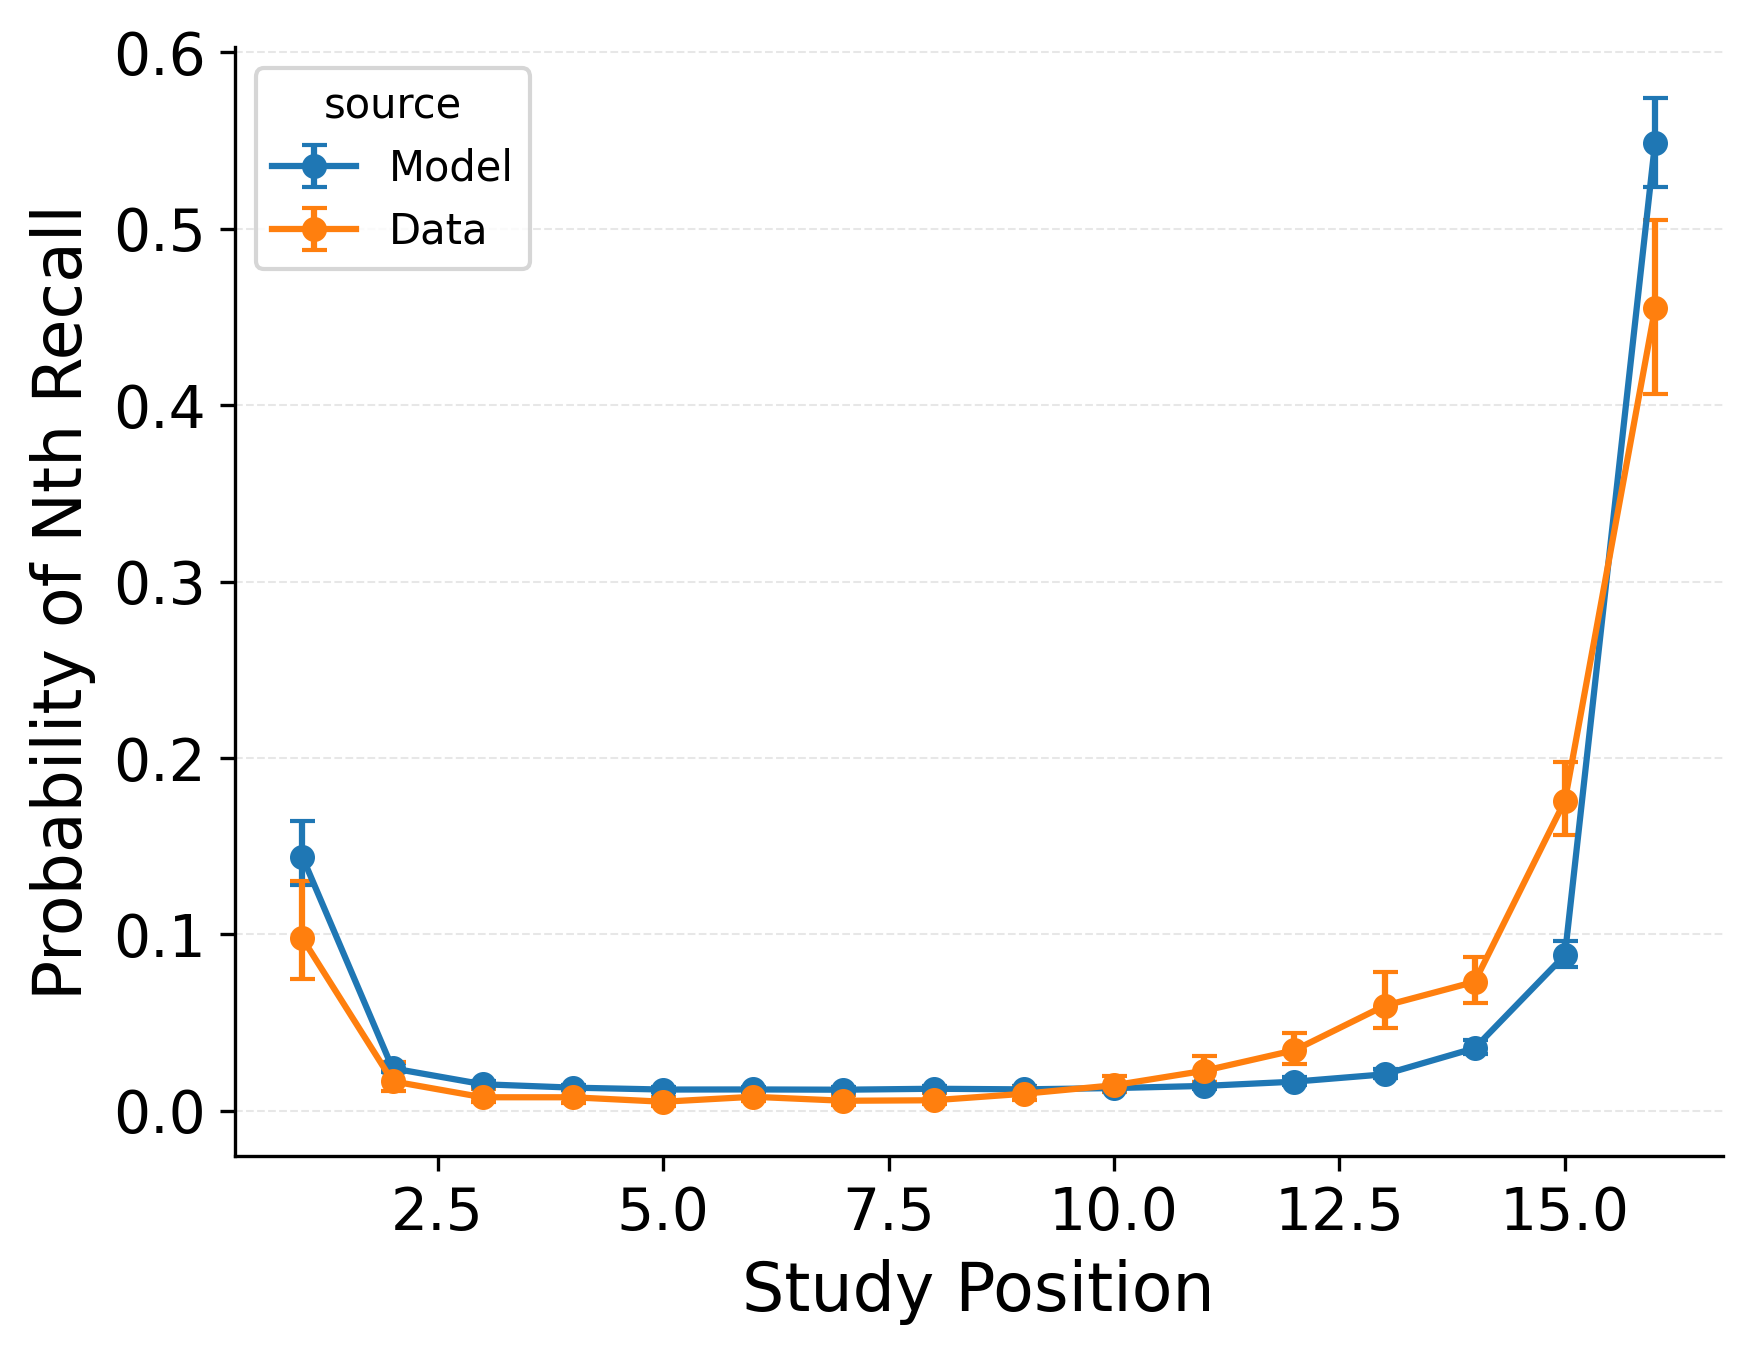
\includegraphics{figures/HealeyKahana2014_BaseCMR_Fitting_pnr.png}\end{minipage}%
%
\begin{minipage}{0.33\linewidth}
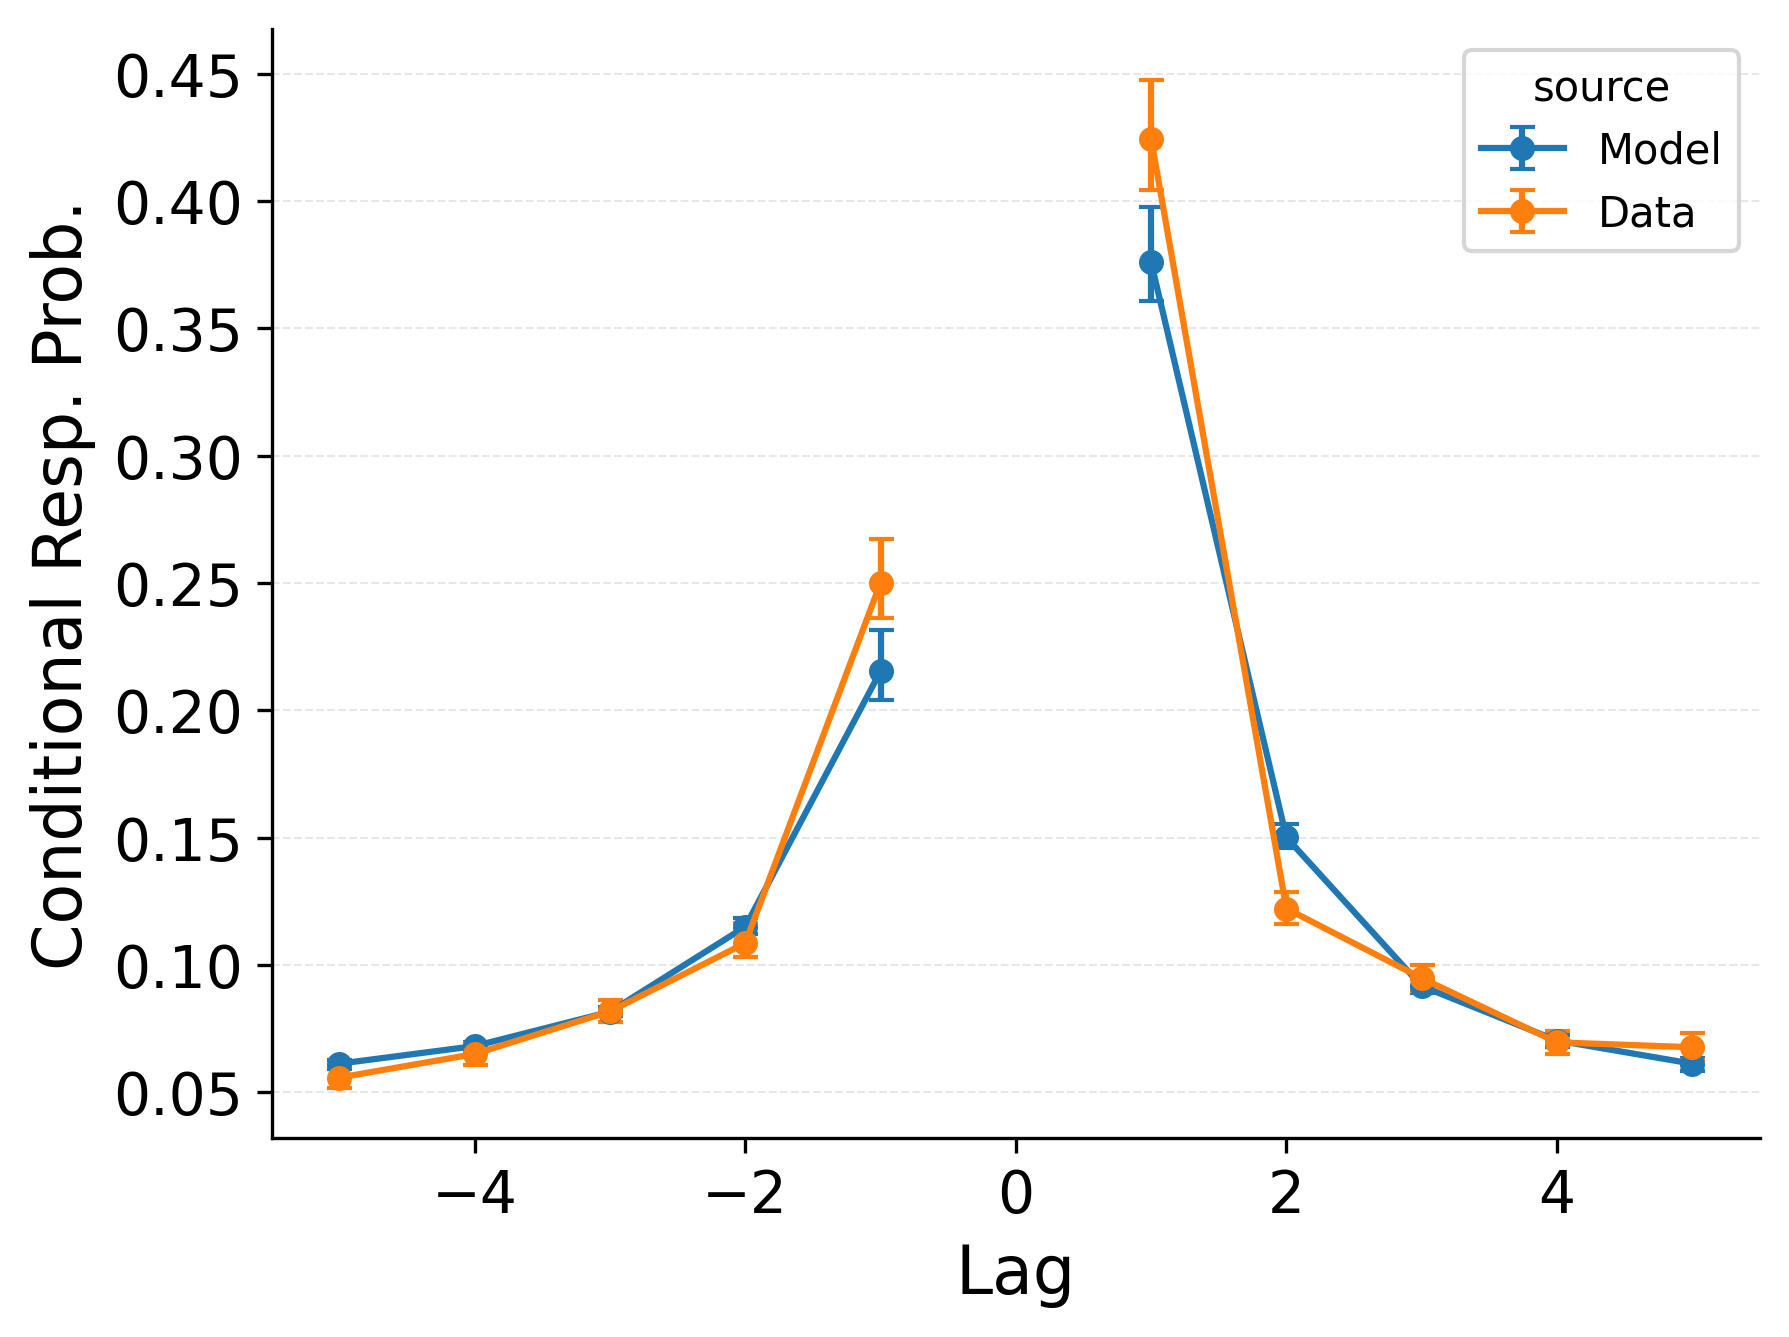
\includegraphics{figures/HealeyKahana2014_BaseCMR_Fitting_crp.png}\end{minipage}%
%
\begin{minipage}{0.33\linewidth}
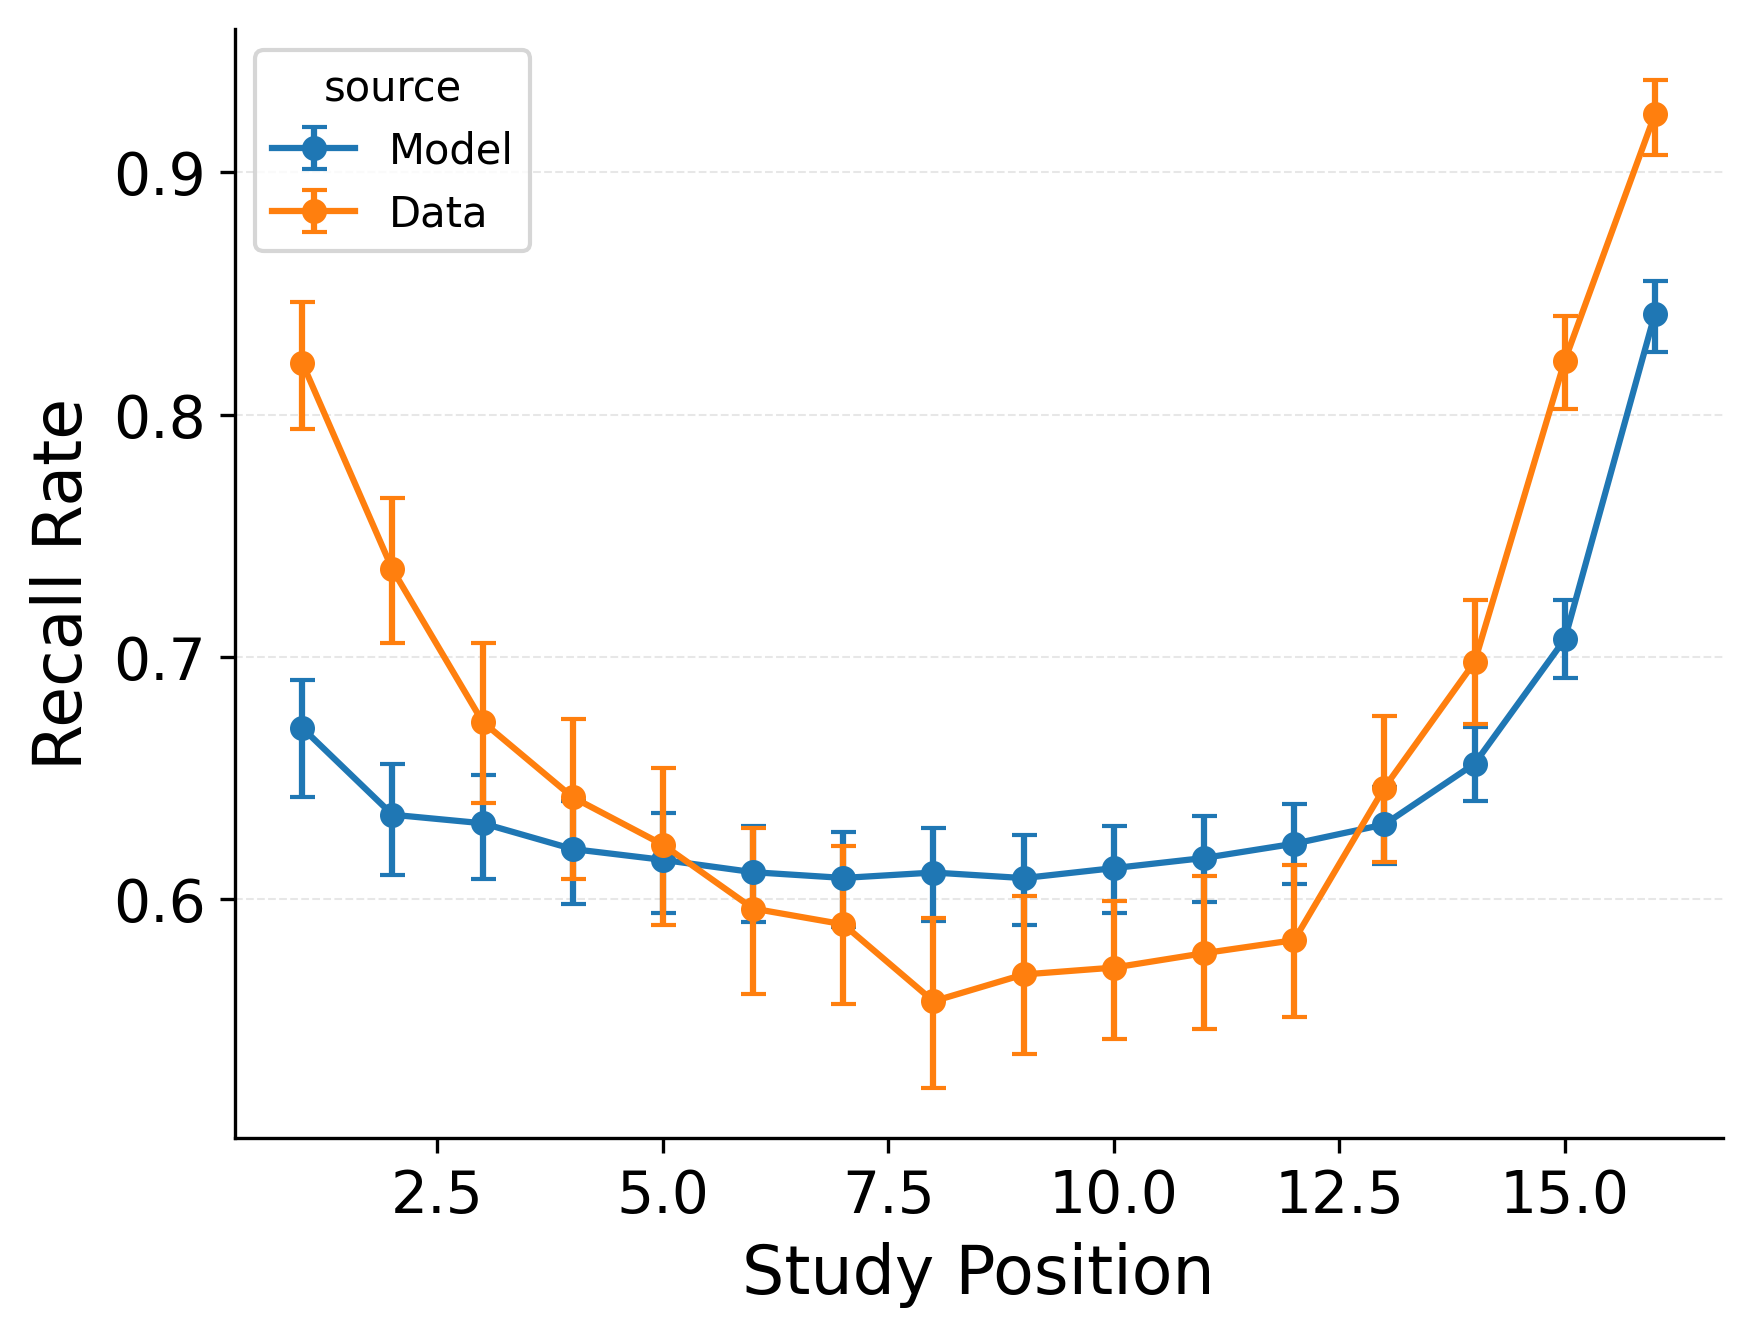
\includegraphics{figures/HealeyKahana2014_BaseCMR_Fitting_spc.png}\end{minipage}%

\end{figure}%

Our first evaluation uses the Healey and Kahana
(\citeproc{ref-healey2014memory}{2014}) subset of the PEERS free recall
dataset. Using the overall goodness of fit for each model variant,
standard CMR provides the best fit at the group level (see
Table~\ref{tbl-fits}) as well as for 100\% of individual participants.
This is no surprise, as CMR uses more parameters and was designed to
capture free recall phenomena while CRU was developed for serial recall
tasks. Our focus instead is in demonstrating how specific model
mechanisms improve CRU's fit to the benchmark behavioral phenomena of
free recall: serial position effects, recall initiation effects, and
temporal organizational effects, as depicted in Figure~\ref{fig-cmr}.

A serial position analysis Figure~\ref{fig-cmr} demonstrates both a
primacy effect (a memorability advantage for early-list items) and a
recency effect (a memorability advantage for late-list items). These
memorability advantages are also apparent in the distribution of first
recalls Figure~\ref{fig-cmr}. In this dataset, a recency effect is
particularly pronounced in the distribution of first recalls;
participants usually start recall with the last item from a study list,
but sometimes start with the first item. By comparison, the serial
position curve shows a more balanced trade-off between primacy and
recency effects.

Two mechanisms allow CMR to capture the interplay between primacy and
recency effects. First, CMR leverages the associative primacy gradient
mechanism modulating learning rates in the context-to-feature memory
(\(\phi_\text{s}\), \(\phi_\text{d}\)) to enhance the memorability of
early-list items. Second, CMR recovers the start-of-list context with a
dedicated context integration parameter (\(\beta_\text{start}\)). Both
mechanisms influence the initiation of recall and the overall serial
position curve, but they have differential effects on these two stages.
The \(\beta_\text{start}\) parameter is most influential at recall
initiation, while the associative primacy gradient influences the
primacy effect throughout retrieval. These mechanisms together allow CMR
to capture both the distribution of first recalls and the overall serial
position curve.

A focal concern of retrieved-context models is the lag-contiguity
effect, the tendency to successively recall items that were presented
close together in time (\citeproc{ref-kahana1996associative}{Kahana,
1996}, \citeproc{ref-kahana2020computational}{2020}). These models
capture this effect by reinstating the temporal context associated with
a just-recalled item (step 1) and then using that updated context to cue
other items (step 2). In free recall, the lag-contiguity effect is
bidirectional but asymmetric, favoring forward transitions over backward
ones. To capture all aspects of the lag-contiguity effect, CMR primarily
uses its feature-to-context memory to reinstate the context associated
with a just-recalled item and then its context-to-feature memory to
activate items associated with its newly updated context. The \(\gamma\)
parameter influences context reinstatement by weighting the influence of
pre-experimental and experimental associations in the feature-to-context
memory. CMR's parameters \(\delta\) and \(\alpha\) conversely configure
pre-experimental context-to-feature memory to influence the extent to
which retrieval of items associated with the current context is focused
on nearby or distant neighbors of the last recalled item. Together,
these parameters yield the characteristic forward-biased yet
bidirectional pattern observed in free recall.

CMR exhibits some limitations capturing these phenomena, underpredicting
the primacy effect in the serial position curve. CMR's ability to
account for performance using this dataset has been evaluated before
(\citeproc{ref-healey2014memory}{Healey \& Kahana, 2014};
\citeproc{ref-morton2016predictive}{Morton \& Polyn, 2016}); depending
on whether CMR is fit to summary statistics or to individual response
sequences, and on how many rerolls of the differential evolution fitting
algorithm are used, CMR's exact fit to these phenomena can vary. Recent
work suggests that a mixture model, in which a given trial either has
support for the end-of-list items or support for the start-of-list
items, may better capture the dynamics of recall initiation
(\citeproc{ref-osth2019using}{Osth \& Farrell, 2019}). Addressing these
limitations and further exploring these interactions are outside the
scope of this paper and reflect continuing challenges in modeling free
recall phenomena. These simulation results demonstrate the ability of
standard CMR to capture key free-recall phenomena, establishing a
baseline that can be built upon in future work. We now turn to CRU and
evaluate how its streamlined implementation impacts its ability to
capture these phenomena.

\subsection{Addressing Serial Position Effects in Recall Initiation and
Overall}\label{addressing-serial-position-effects-in-recall-initiation-and-overall}

\begin{figure}

\caption{\label{fig-initiation}Summary statistic fits of baseline CRU
(\textbf{Top}), CRU with free start context integration rate
\(\beta_\text{start}\) (\textbf{Middle}), and CRU freeing both start
context integration rate (\(\beta_\text{start}\)) and primacy gradient
(\(\phi_\text{s}\) and \(\phi_\text{d}\)) parameters (\textbf{Bottom})
to PEERS free recall data. \textbf{Left}: probability of recall
initiation by serial position. \textbf{Middle}: conditional response
probability as a function of lag. \textbf{Right}: recall probability by
serial position.}

\begin{minipage}{0.33\linewidth}
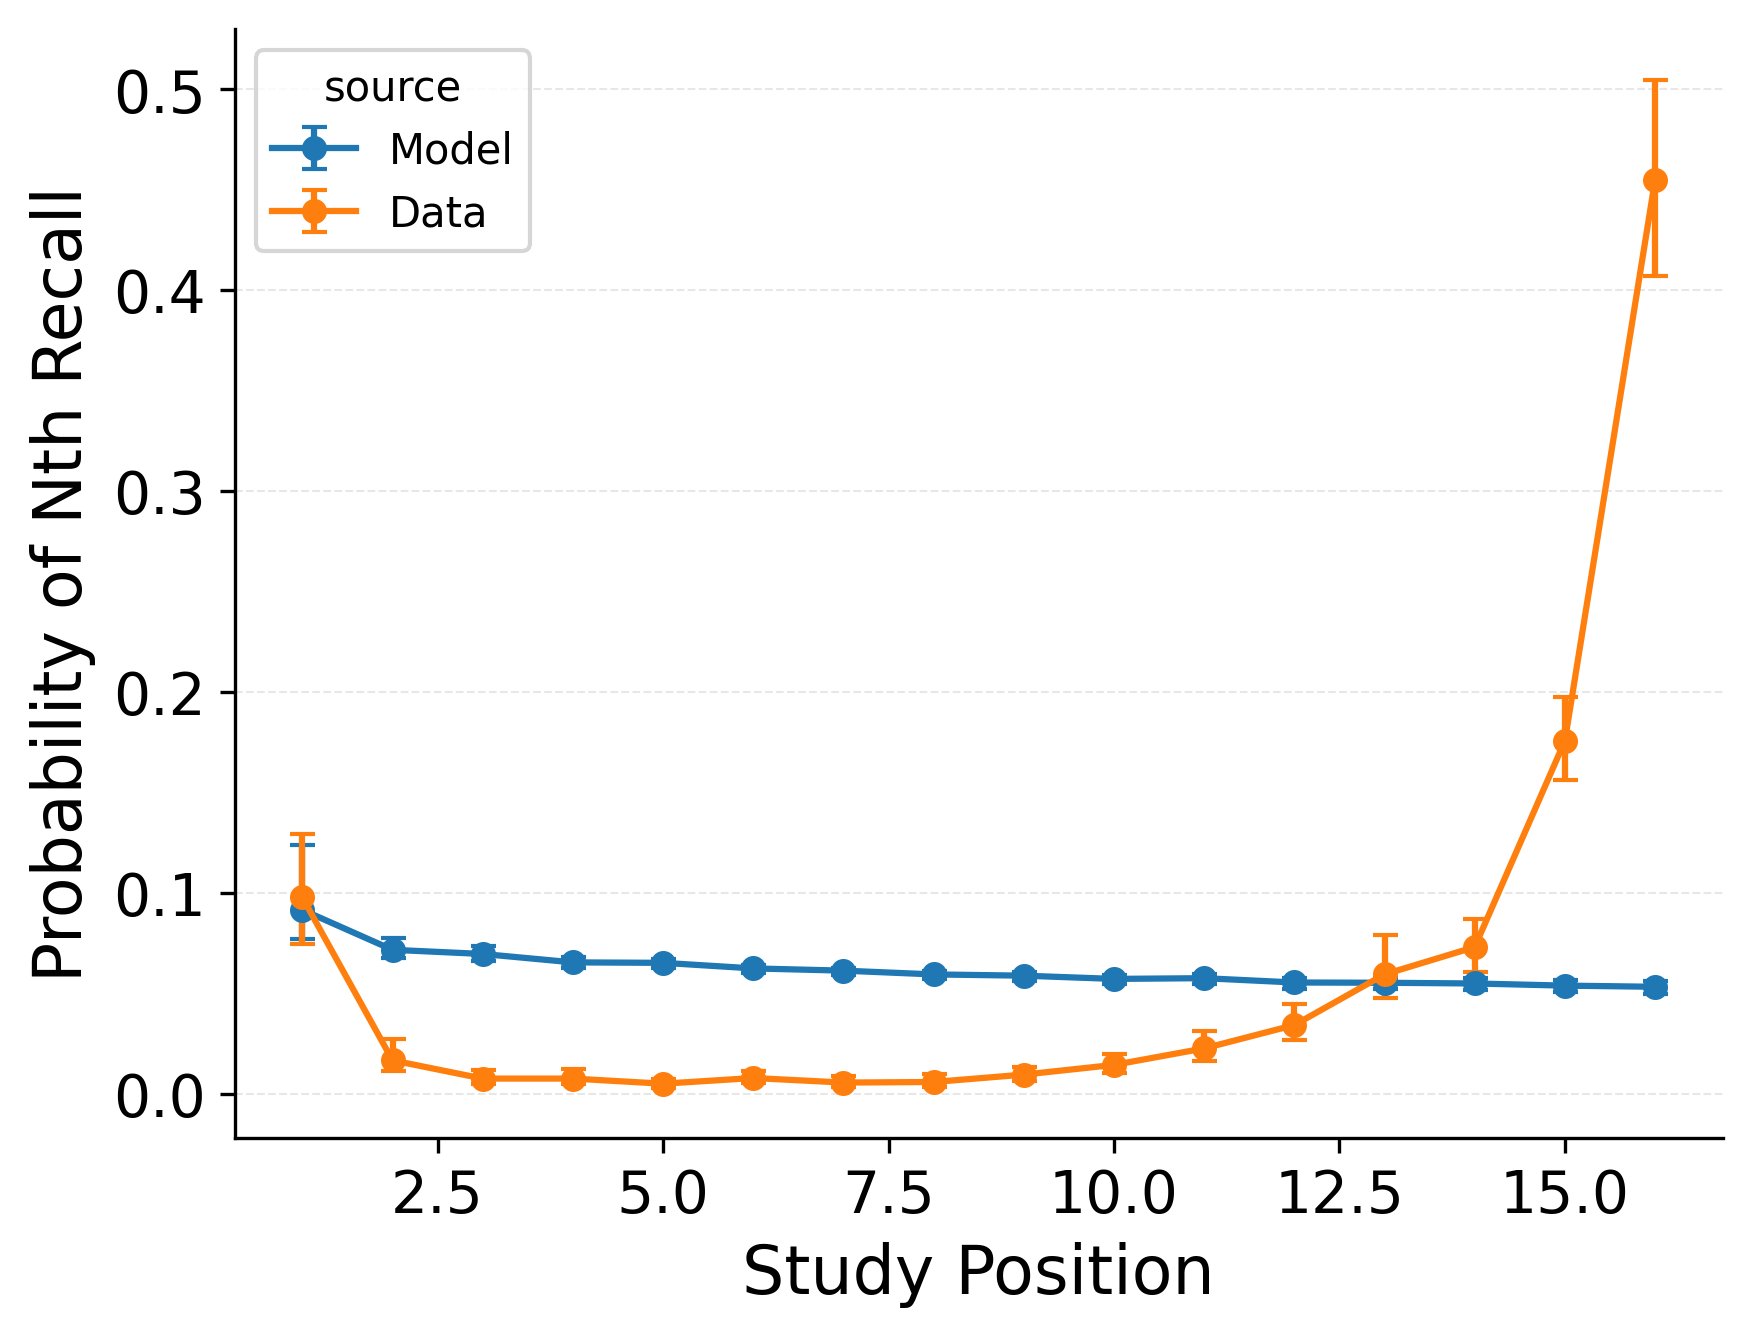
\includegraphics{figures/HealeyKahana2014_BaseCRU_Fitting_pnr.png}\end{minipage}%
%
\begin{minipage}{0.33\linewidth}
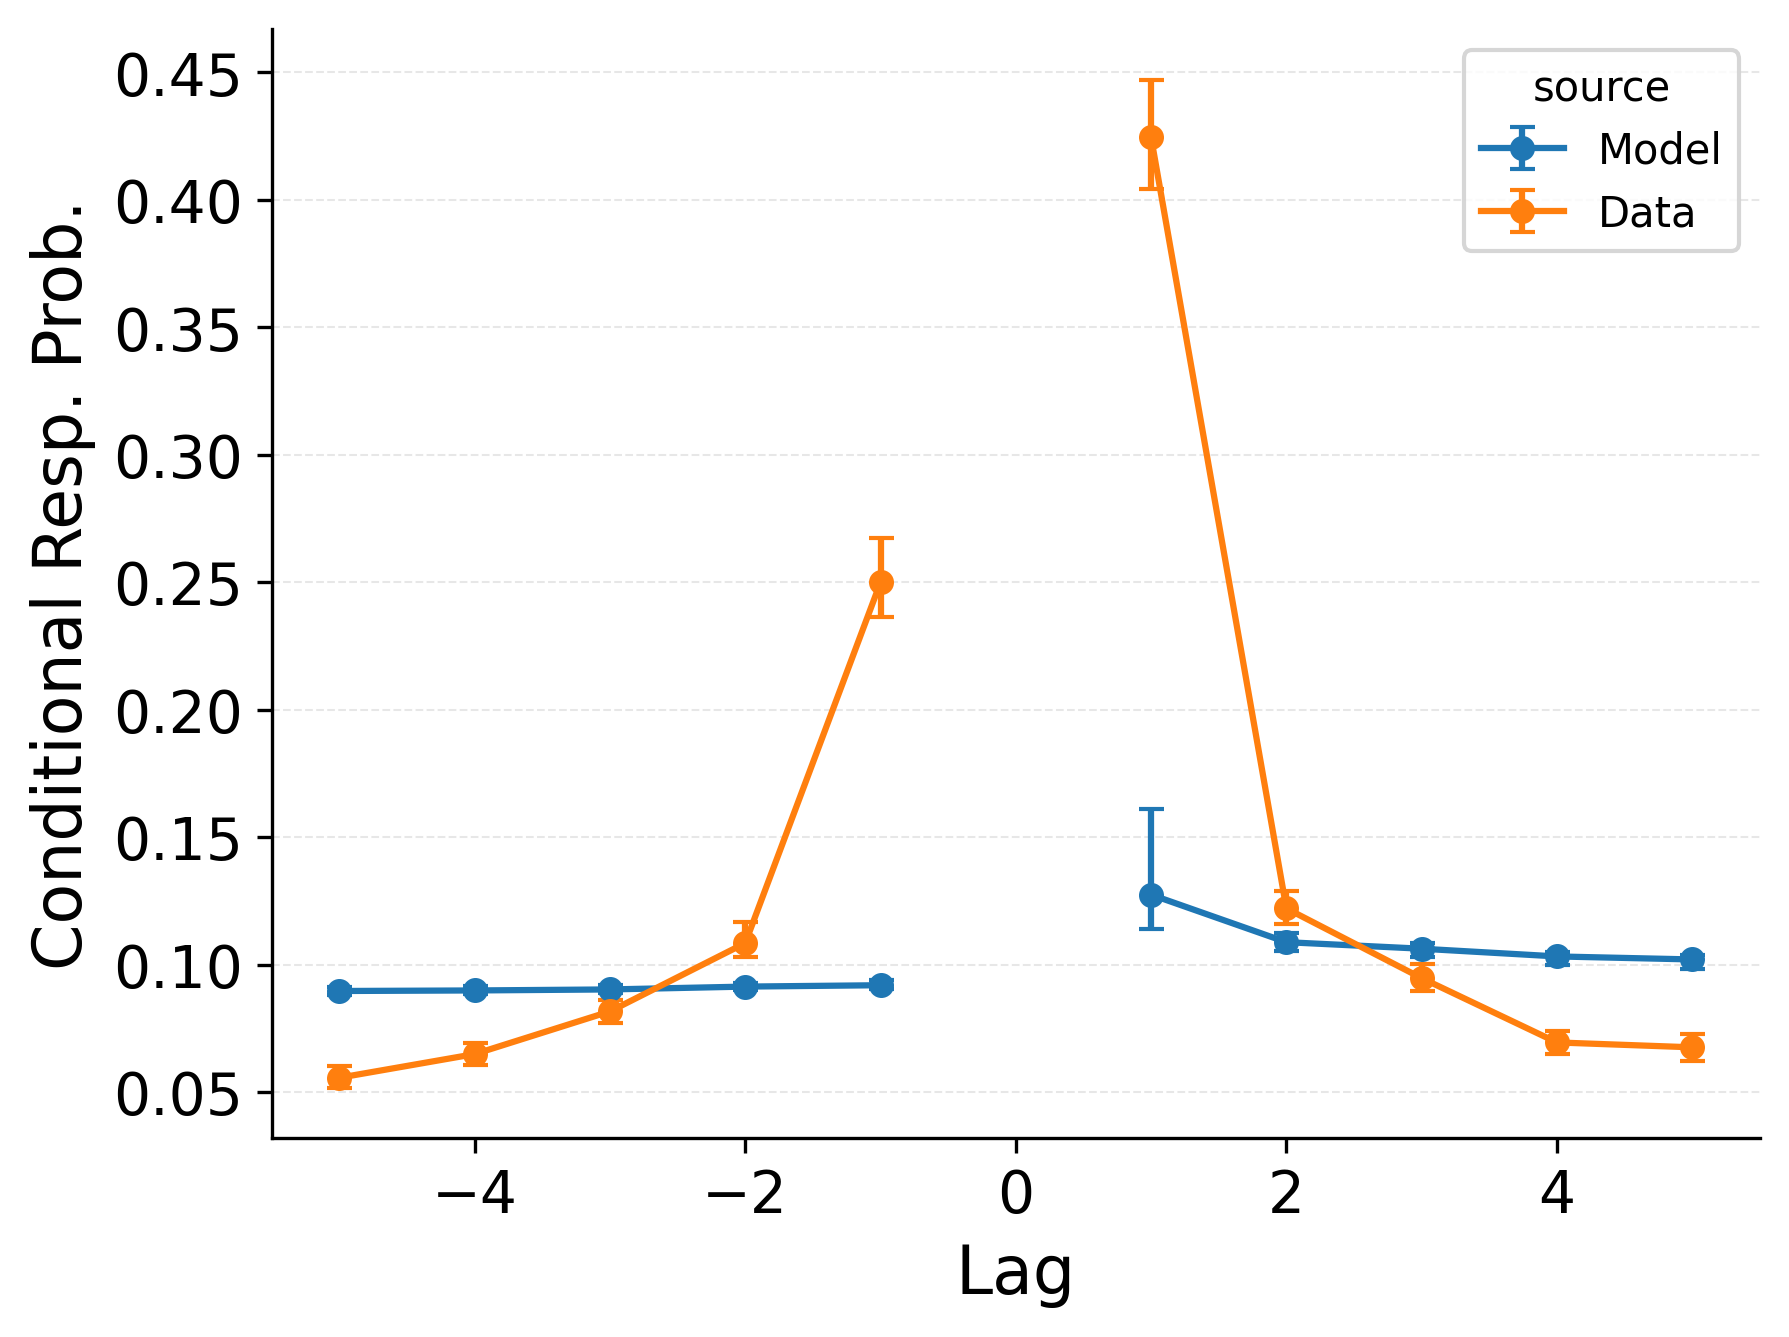
\includegraphics{figures/HealeyKahana2014_BaseCRU_Fitting_crp.png}\end{minipage}%
%
\begin{minipage}{0.33\linewidth}
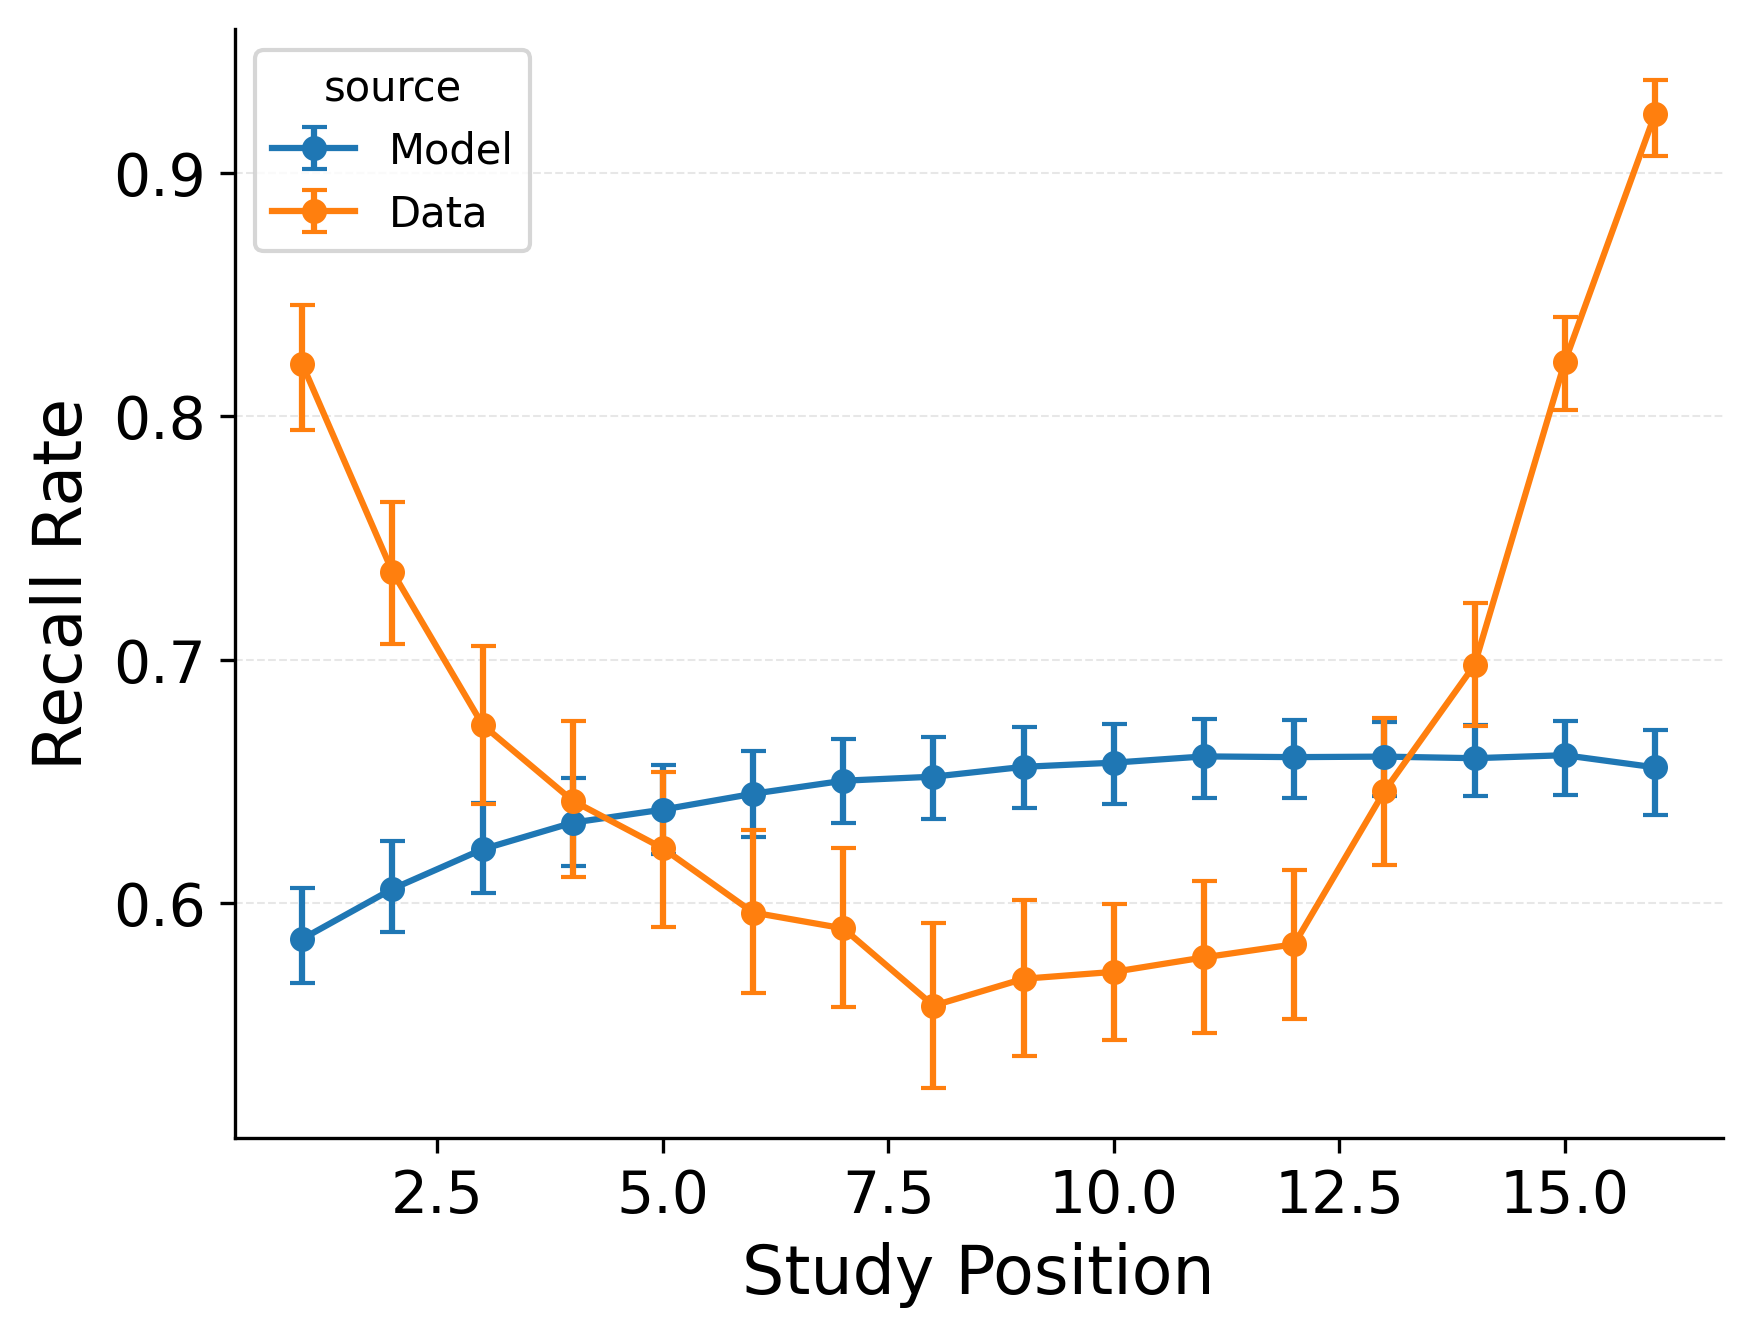
\includegraphics{figures/HealeyKahana2014_BaseCRU_Fitting_spc.png}\end{minipage}%
\newline
\begin{minipage}{0.33\linewidth}
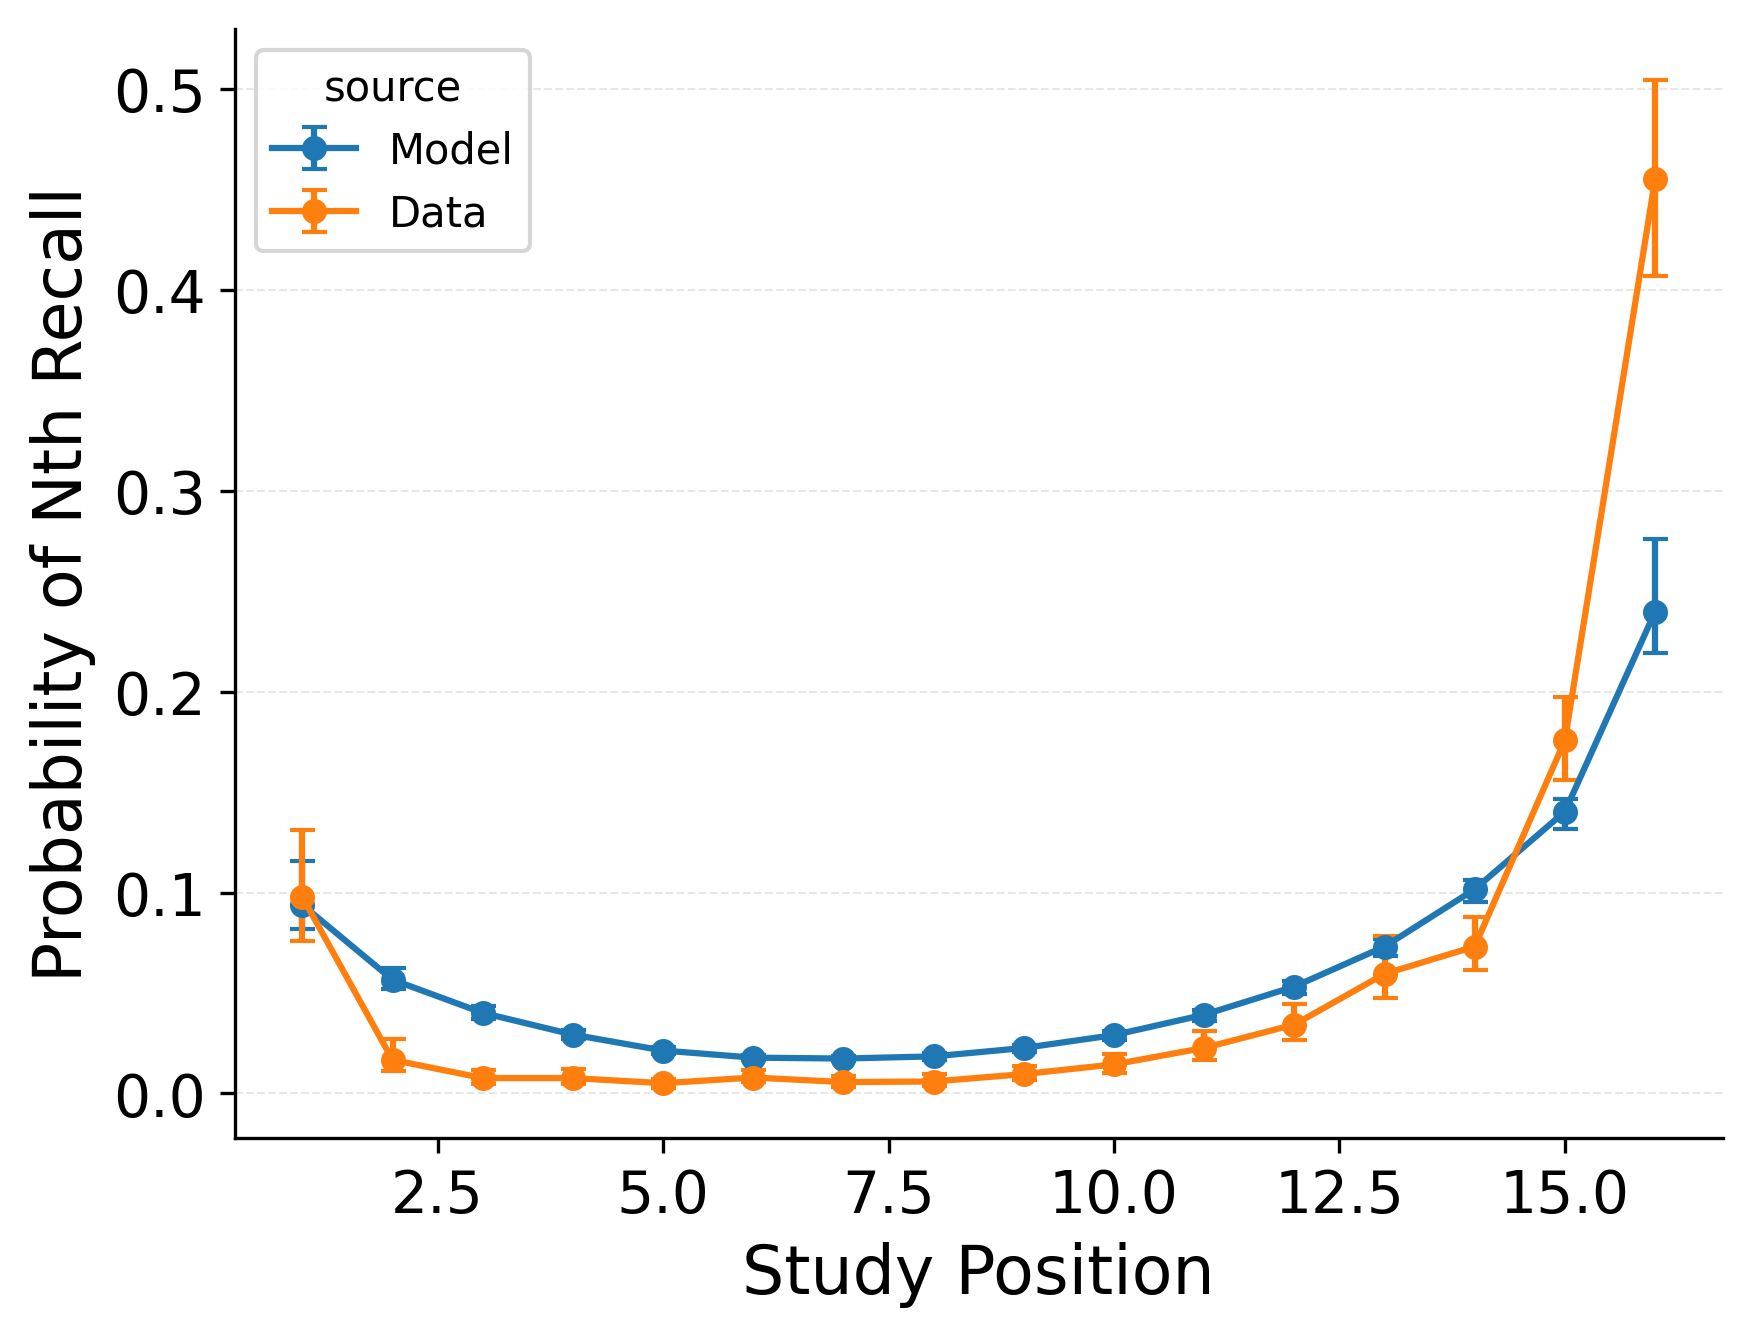
\includegraphics{figures/HealeyKahana2014_CRU_with_Free_Start_Drift_rate_Fitting_pnr.png}\end{minipage}%
%
\begin{minipage}{0.33\linewidth}
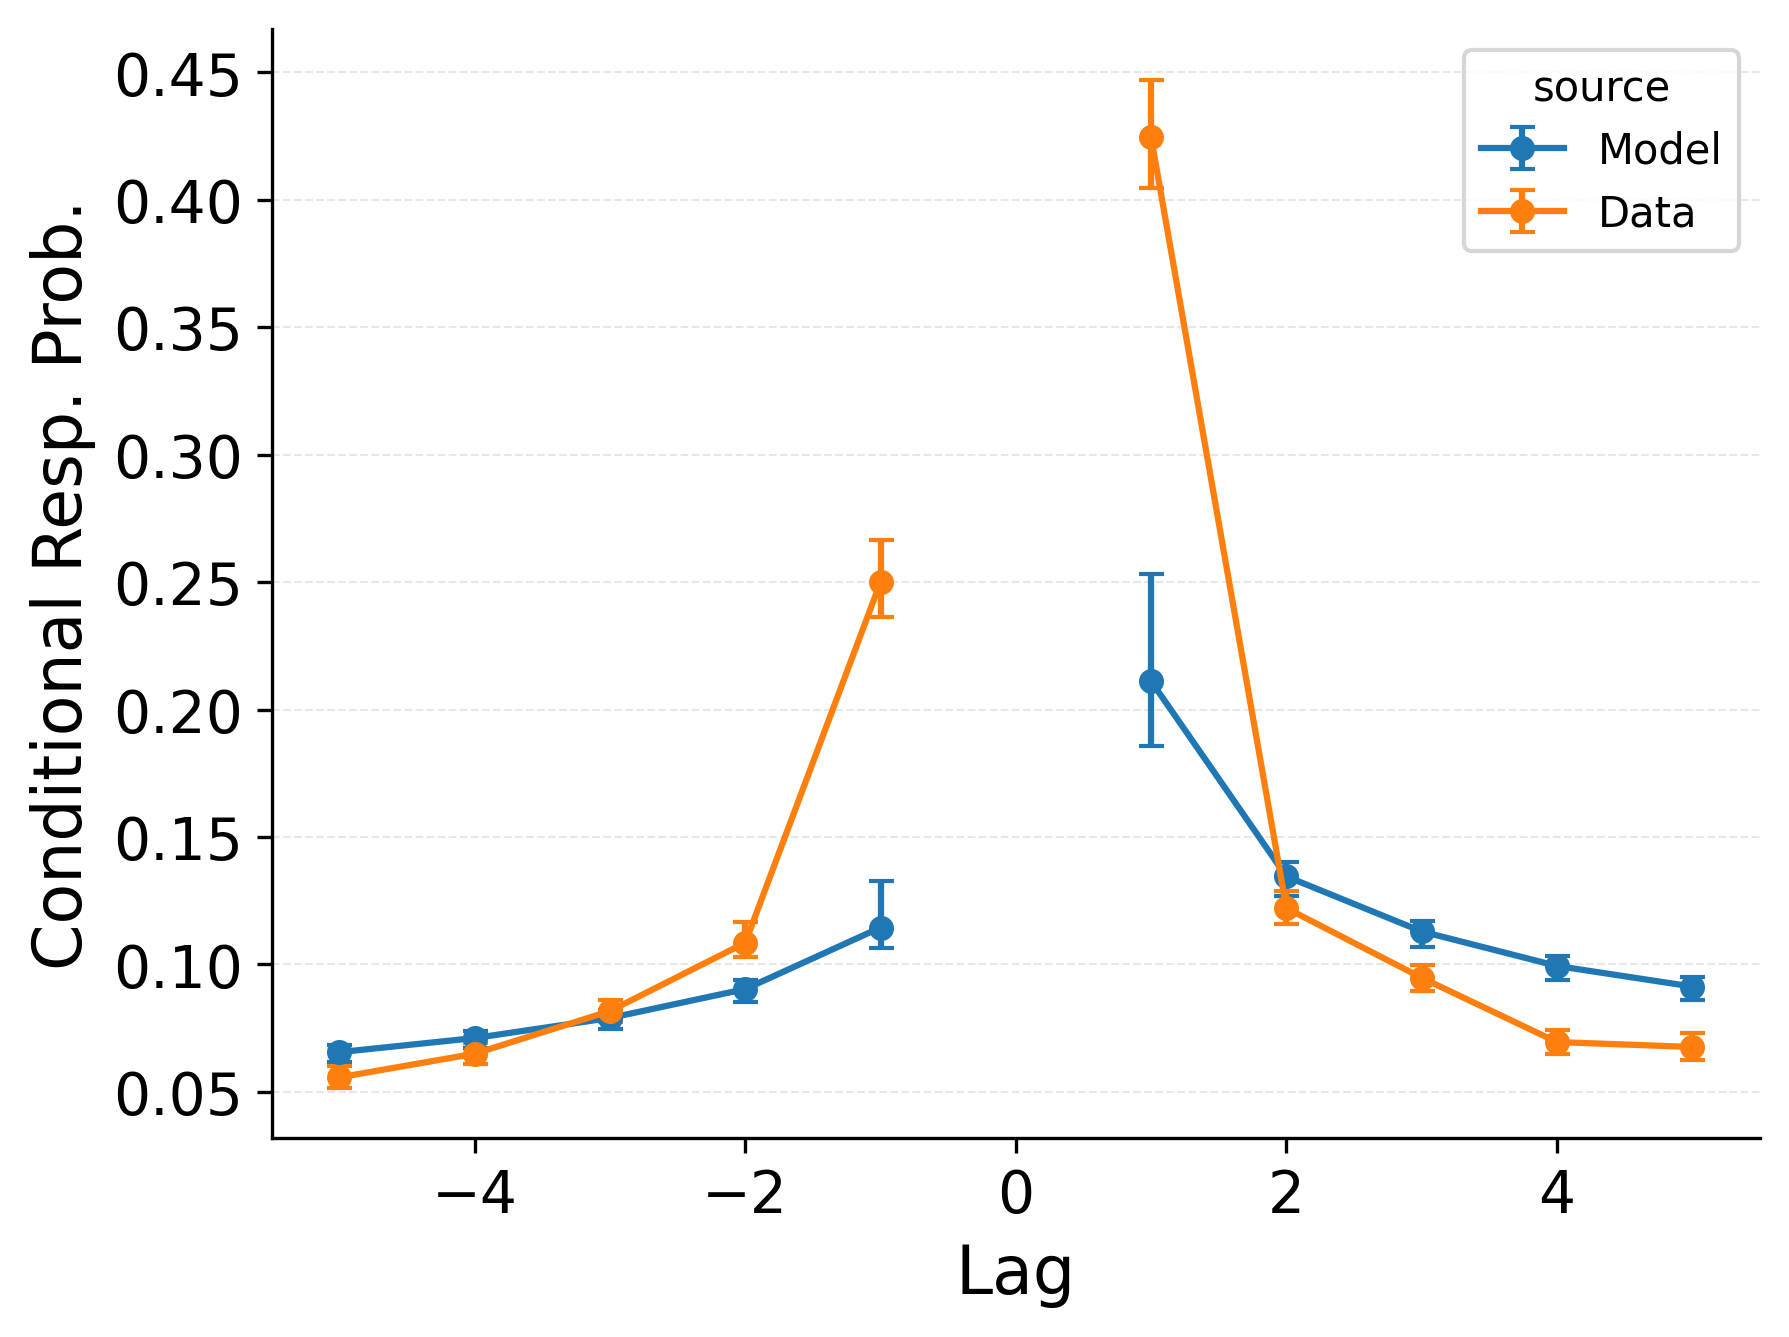
\includegraphics{figures/HealeyKahana2014_CRU_with_Free_Start_Drift_rate_Fitting_crp.png}\end{minipage}%
%
\begin{minipage}{0.33\linewidth}
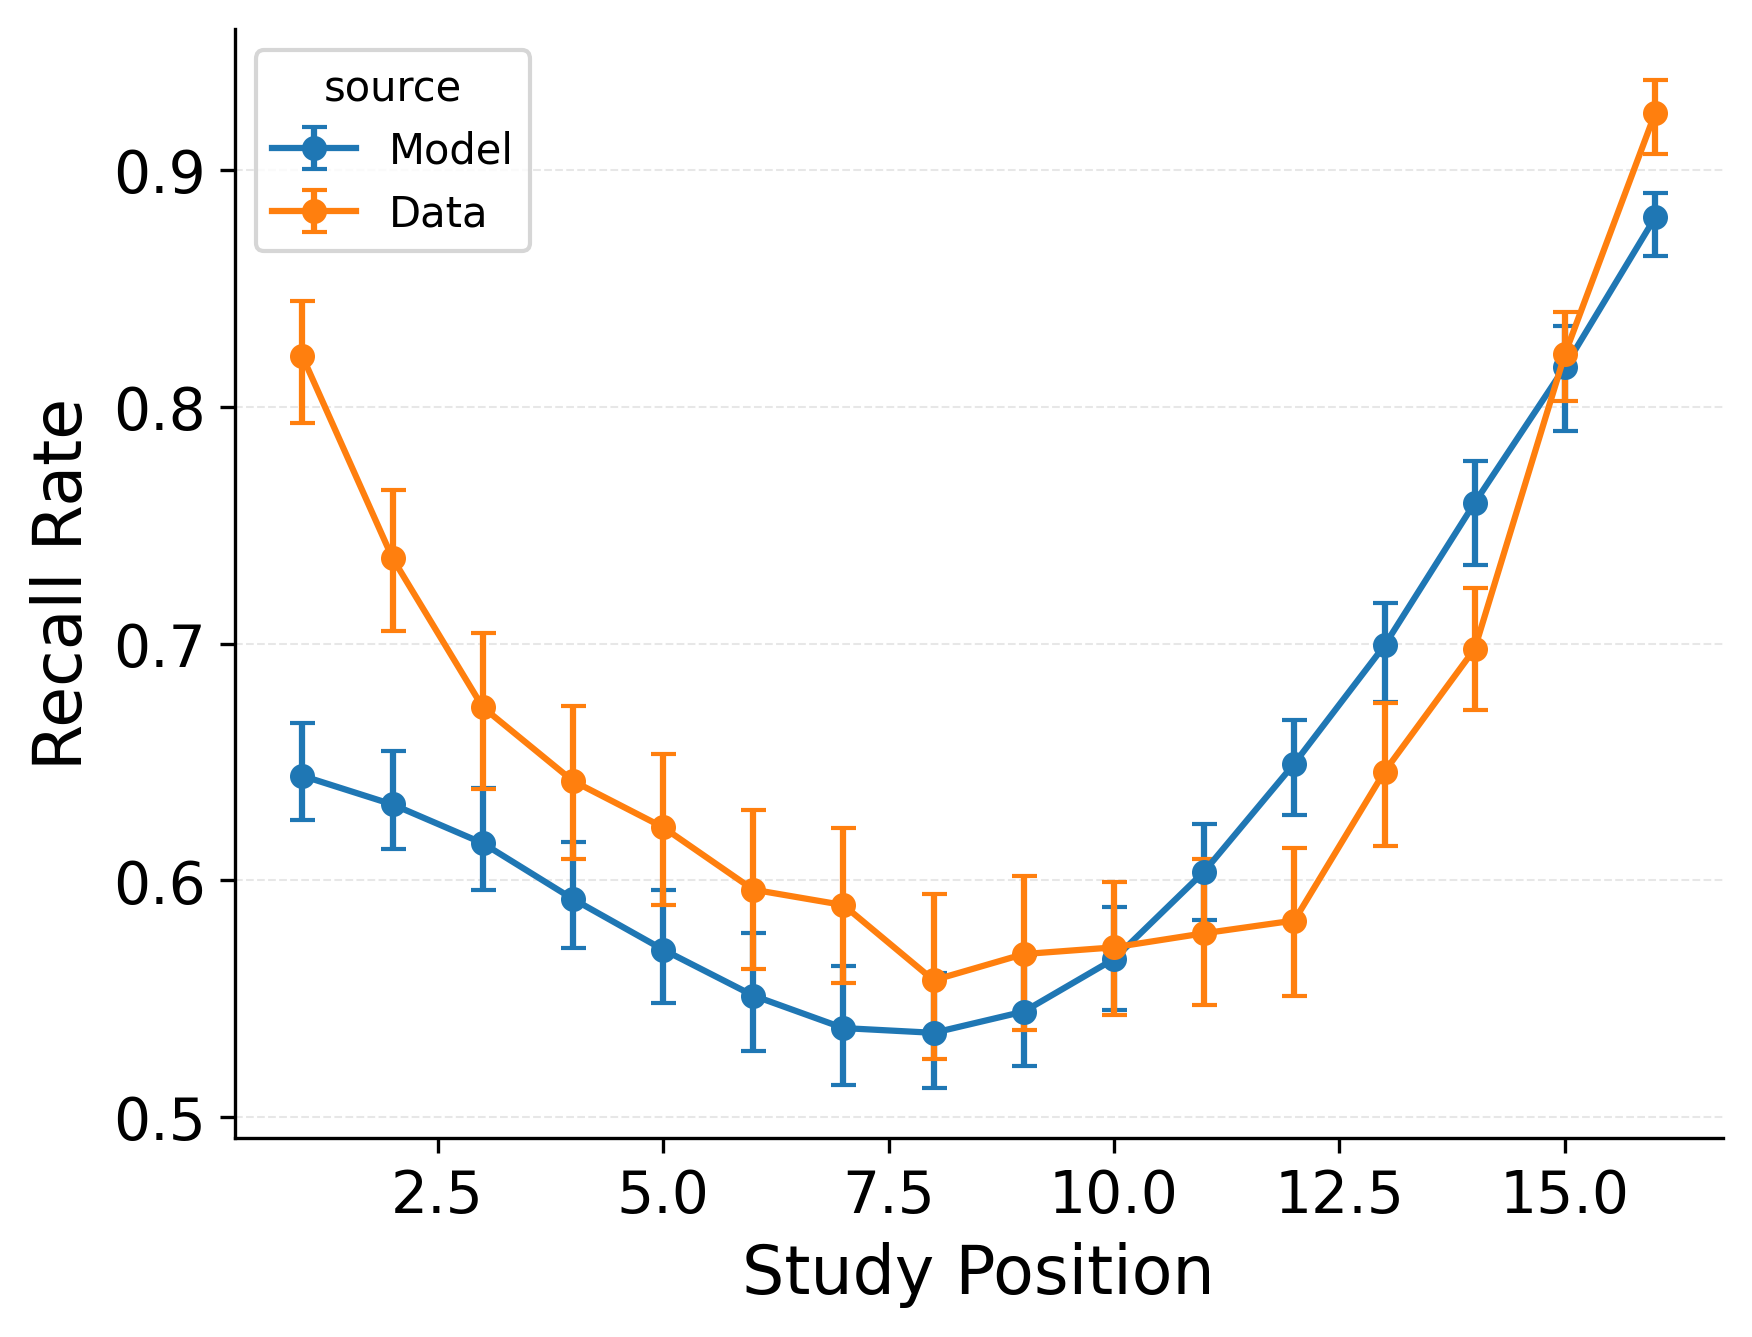
\includegraphics{figures/HealeyKahana2014_CRU_with_Free_Start_Drift_rate_Fitting_spc.png}\end{minipage}%
\newline
\begin{minipage}{0.33\linewidth}
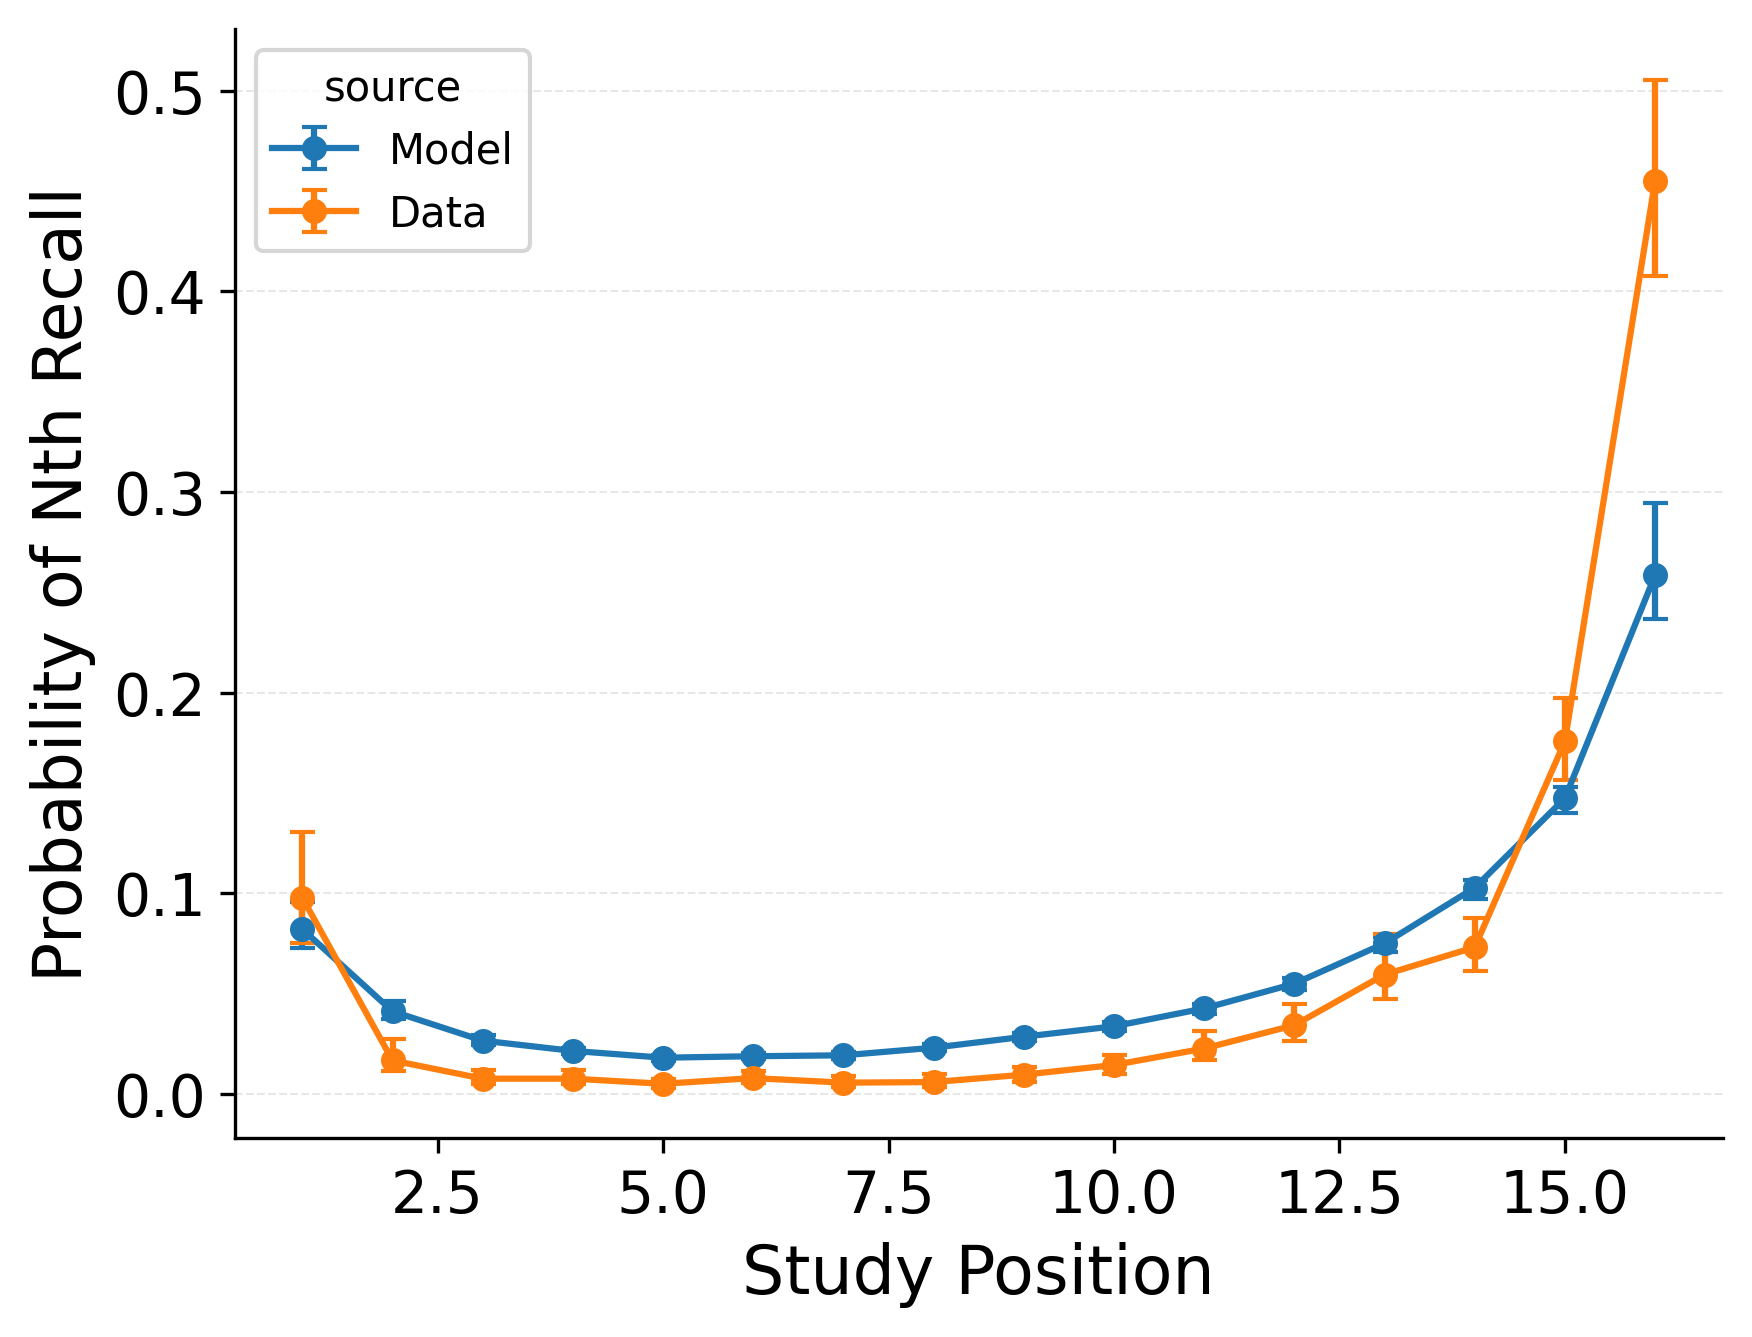
\includegraphics{figures/HealeyKahana2014_CRU_with_Primacy_and_StartDrift_Fitting_pnr.png}\end{minipage}%
%
\begin{minipage}{0.33\linewidth}
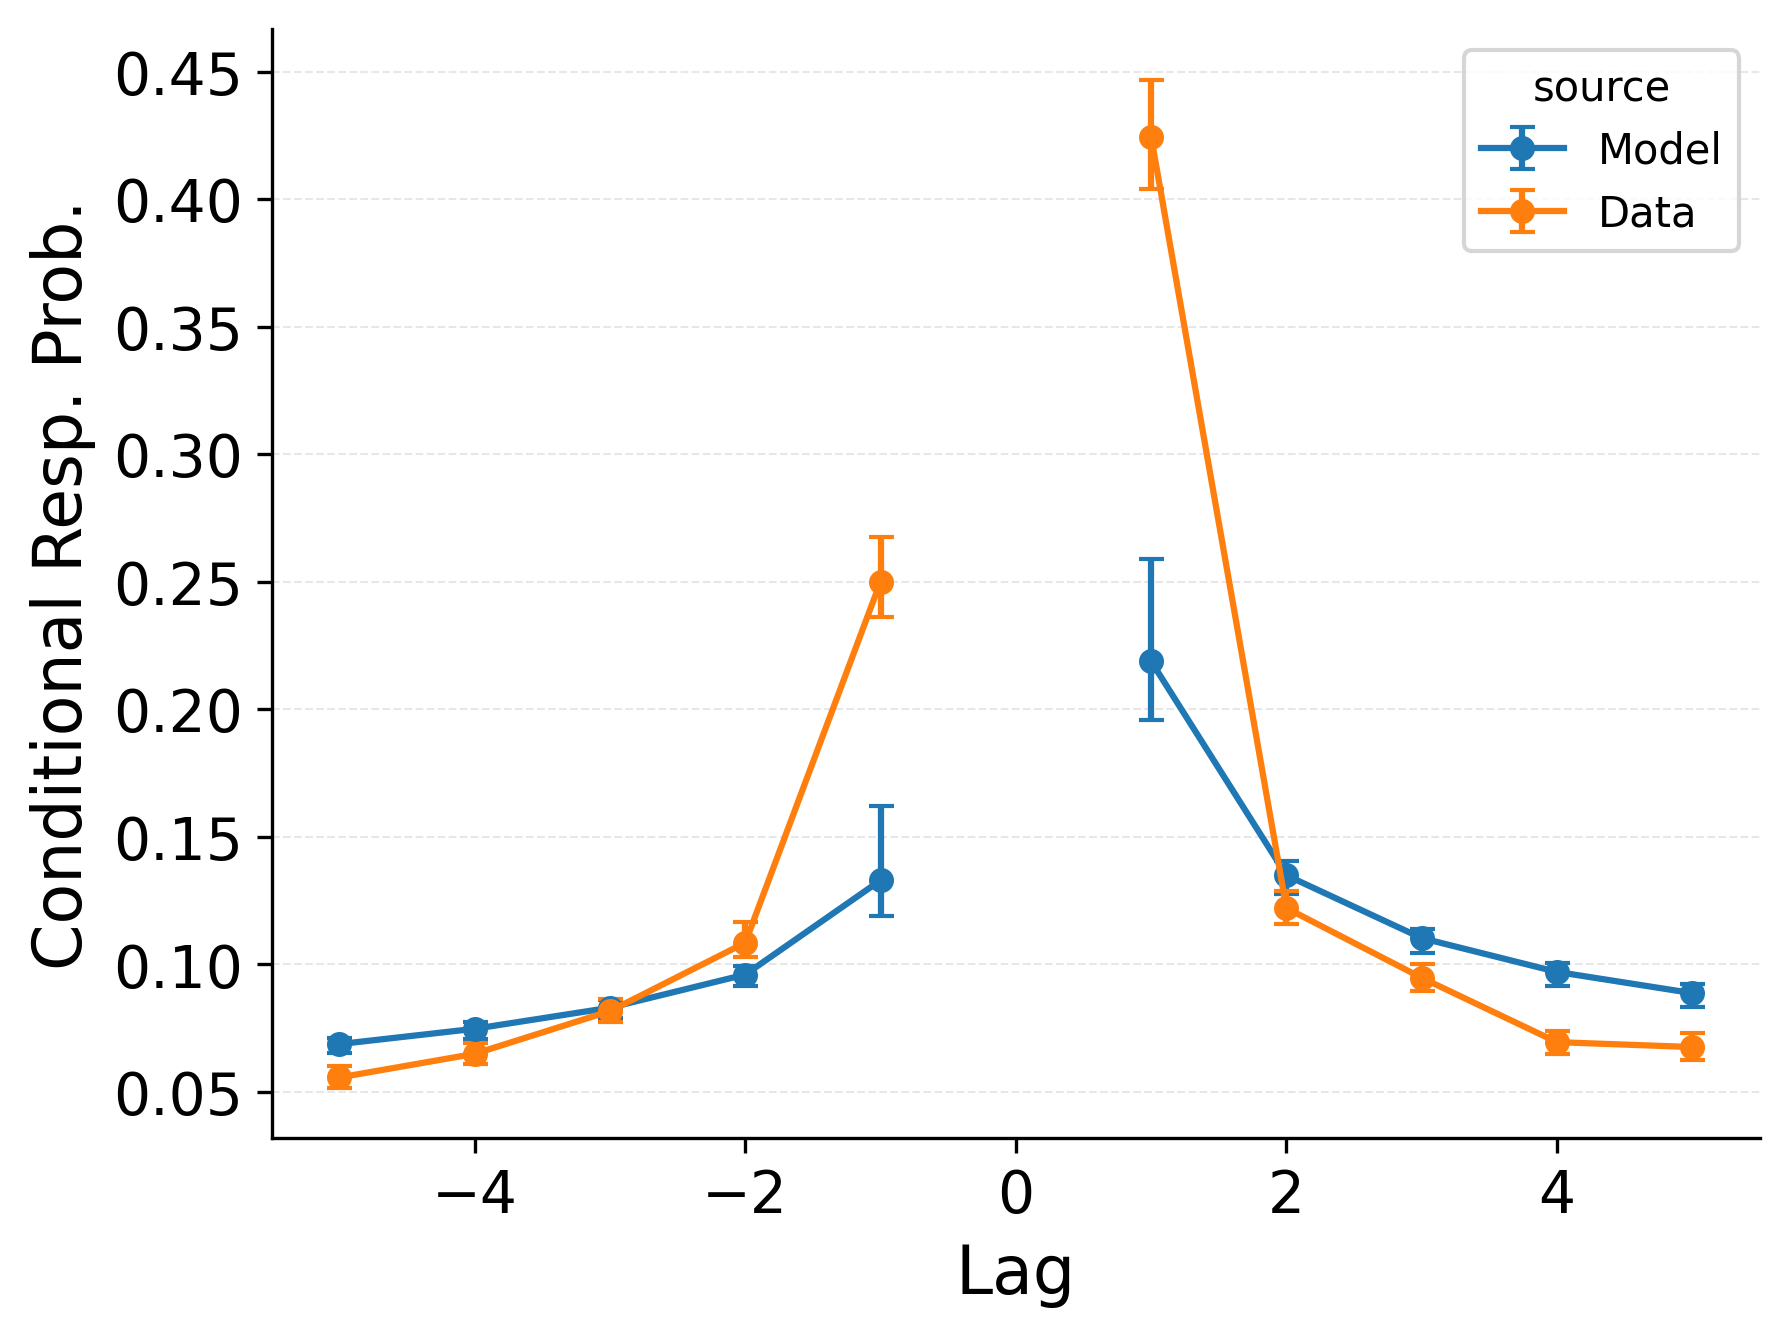
\includegraphics{figures/HealeyKahana2014_CRU_with_Primacy_and_StartDrift_Fitting_crp.png}\end{minipage}%
%
\begin{minipage}{0.33\linewidth}
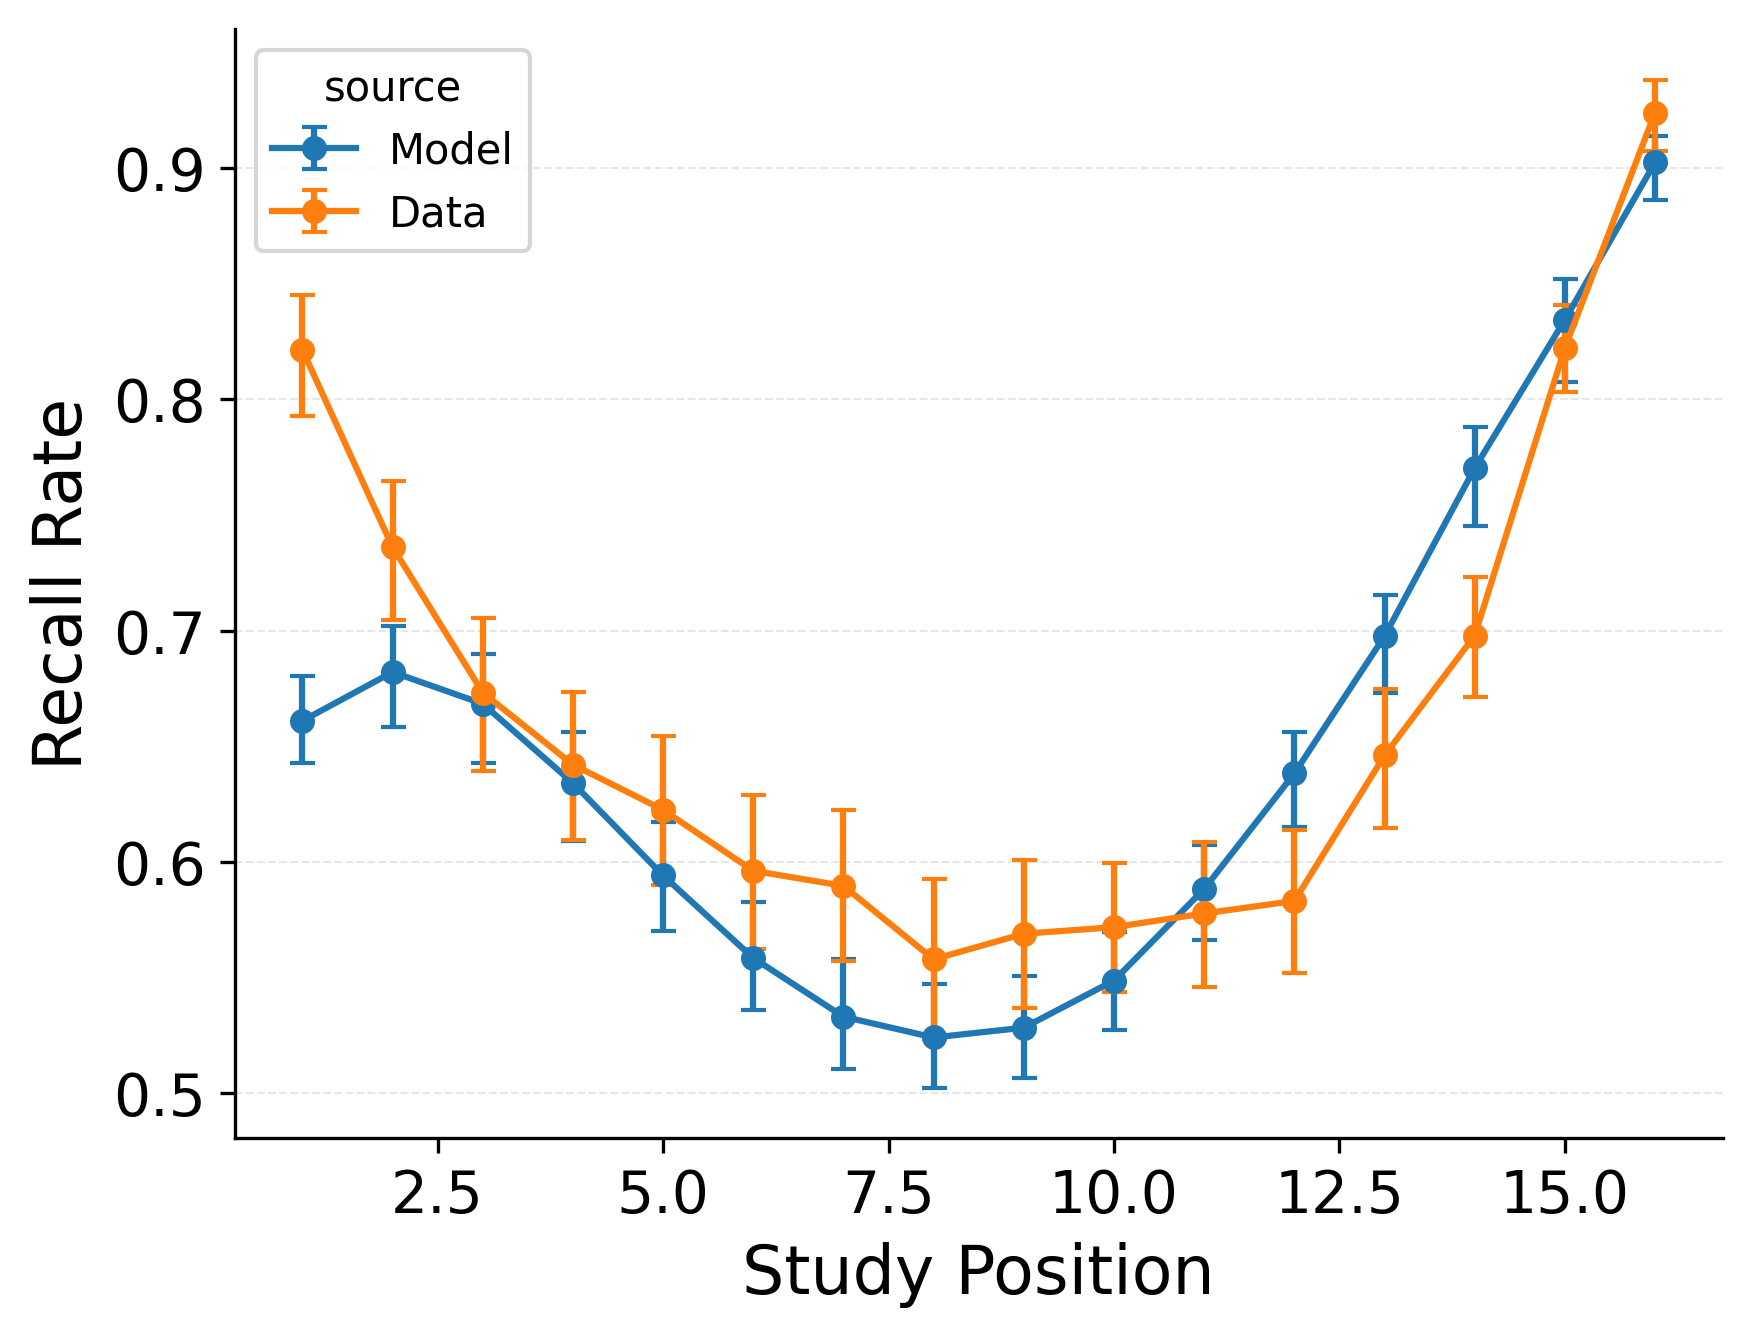
\includegraphics{figures/HealeyKahana2014_CRU_with_Primacy_and_StartDrift_Fitting_spc.png}\end{minipage}%

\end{figure}%

CRU includes most of CMR's core mechanisms. However, CRU's default
start-of-list recall initiation mechanism forces it to strongly
prioritize the start of the list during recall initiation, which causes
its performance to collapse when fit to free recall data exhibiting a
strong recency effect. This failure to capture recall initiation affects
the entire response sequence because transitions in free recall depend
substantially on prior recalls. Allowing CRU to initiate retrieval with
a blend of the end-of-list and start-of-list context according to a
flexible start-of-recall parameter like CMR's \(\beta_\text{start}\)
substantially improves its ability to capture these phenomena
Figure~\ref{fig-initiation}.

Figure~\ref{fig-shiftstart} shows the impact of shifting the start
context integration rate parameter \(\beta_\text{start}\) on the
probability of starting recall by serial position and the recall
probability by serial position for CMR. To perform this simulation, we
fit CMR to each individual participant in the subset of the PEERS
dataset (\citeproc{ref-healey2014memory}{Healey \& Kahana, 2014}) and
then shifted the \(\beta_\text{start}\) parameter from 0 to 1 in
increments of 0.1, repeatedly simulating the model on the same list
structure it was fit to and generating serial position curves and recall
initiation curves. This parameter primarily trades off the strength of
the primacy effect in recall initiation against the strength of the
recency effect, with higher values of \(\beta_\text{start}\) leading to
stronger primacy effects and lower values leading to stronger recency
effects. The serial position curve is sensitive to the value of
\(\beta_\text{start}\) as well since the item retrieval initiates with
affects the trajectory of responses throughout the recall sequence.

We illustrate this point by comparing standard CRU to a CRU variant that
includes CMR's start context integration rate \(\beta_\text{start}\)
parameter as well as a CRU variant that additionally includes CMR's
primacy gradient (\(\phi_\text{s}\) and \(\phi_\text{d}\)) parameters.
Rows 1 and 2 of Figure~\ref{fig-initiation} show simulated benchmark
phenomena for CRU and the first variant, respectively. Fixing
\(\beta_\text{start}\) to 1 leads to fits where CRU predicts no
consistent serial position or lag-contiguity effects, while allowing
\(\beta_\text{start}\) to vary enables CRU to begin to capture these
effects, achieving a U-shaped overall serial position curve, a strong
recency effect in recall initiation, and a bidirectional lag-contiguity
effect. The model still substantially underestimates the primacy effect
in the overall serial position curve, the strength of the recency effect
in recall initiation, and the strength of the lag-contiguity effect, but
these limitations are less severe than when \(\beta_\text{start}\) is
fixed at 1.0.

\begin{figure}

\caption{\label{fig-shiftstart}Simulation of the impact of shifting the
start context integration rate parameter \(\beta_\text{start}\) on the
probability of starting recall by serial position (\textbf{Left}) and
the recall probability by serial position (\textbf{Right}) for CMR.
Using parameters fit to PEERS free recall data, \(\beta_\text{start}\)
is shifted from 0 to 1 in increments of 0.1, with the color of the lines
indicating the value of the parameter.}

\begin{minipage}{0.50\linewidth}
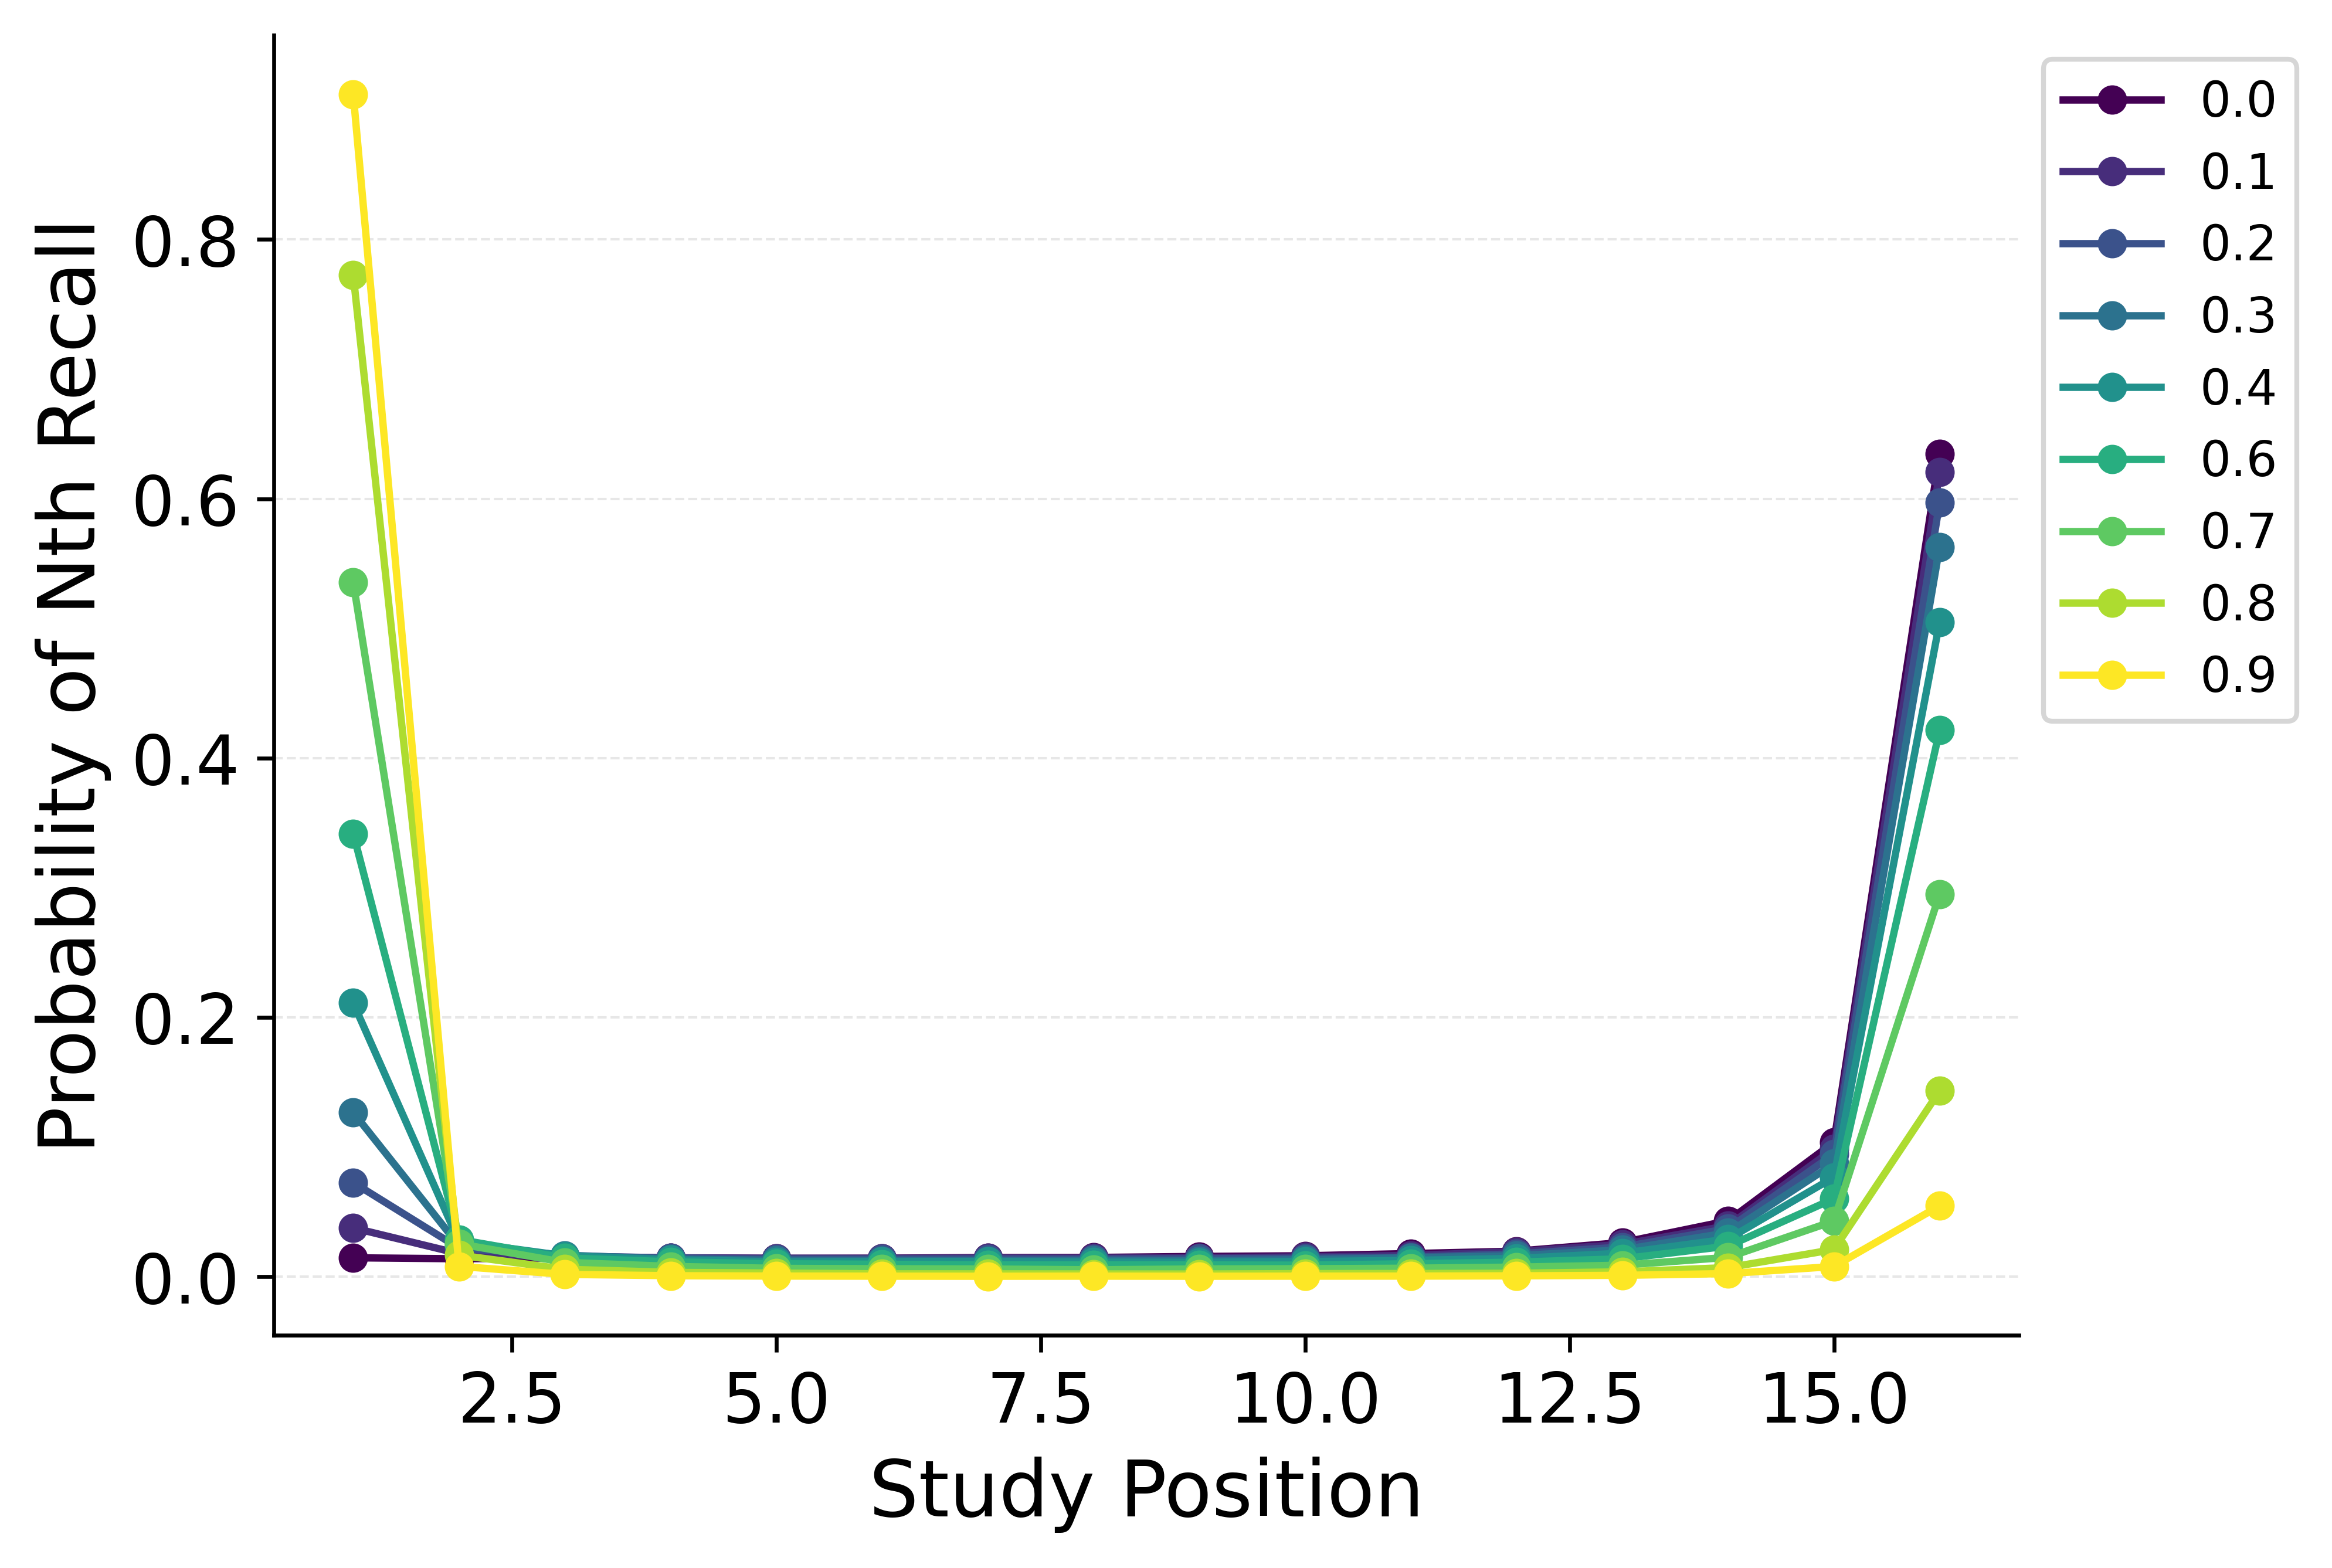
\includegraphics{shifting/BaseCMR_Start_Drift_Rate_Parameter_Shifting_pnr_HealeyKahana2014.png}\end{minipage}%
%
\begin{minipage}{0.50\linewidth}
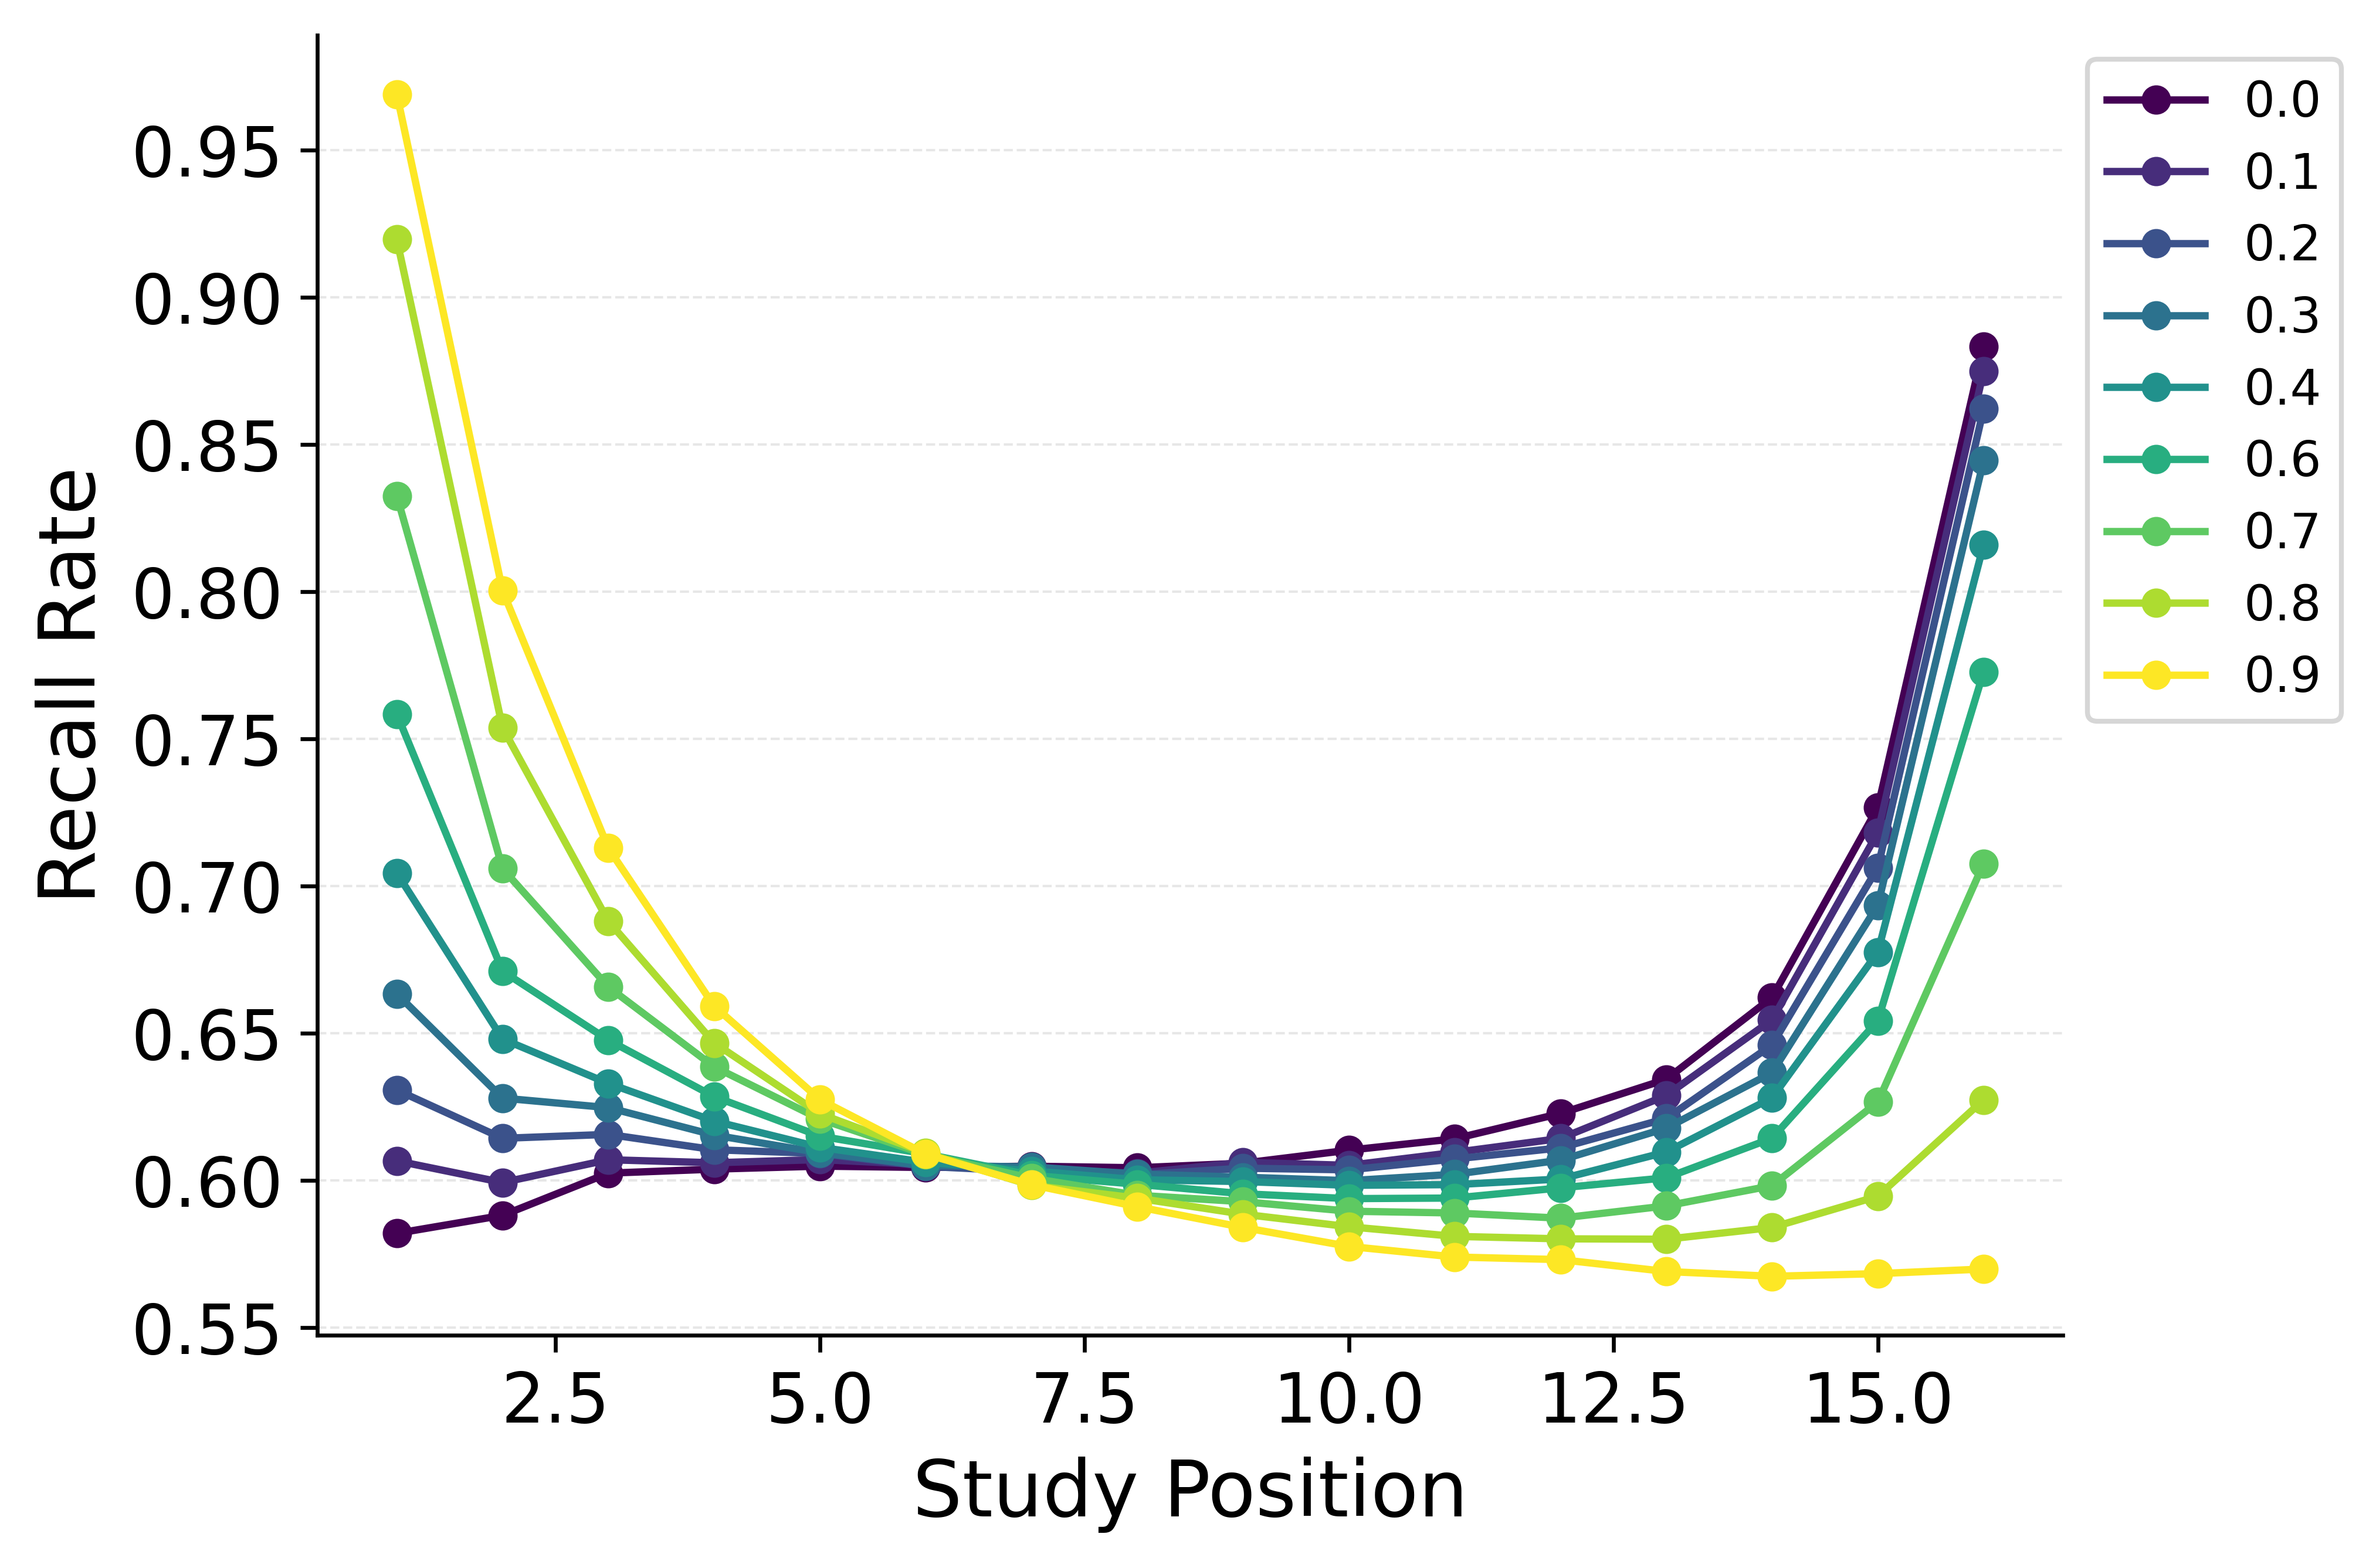
\includegraphics{shifting/BaseCMR_Start_Drift_Rate_Parameter_Shifting_spc_HealeyKahana2014.png}\end{minipage}%

\end{figure}%

Further allowing CRU to include CMR's primacy learning gradient
(\(\phi_\text{s}\) and \(\phi_\text{d}\) parameters) to modulate
context-to-feature memory learning rates to peak at the start of the
study list further improves its performance. This variant is better at
capturing the strength of the primacy effect in the overall serial
position curve Figure~\ref{fig-initiation}, but does not as
substantially improve the model's ability to capture the recency effect
in recall initiation or the lag-contiguity effect.

These differences observed between CRU and CMR in their ability to
address serial position effects may be exaggerated by the exclusion of
an item identification mechanism in CRU addressing free recall. Logan
(\citeproc{ref-logan2021serial}{2021}) accounted for primacy effects in
CRU with \(g_\text{max}\) and \(g_\text{dec}\) parameters that allowed
the model to modulate the sensitivity of item identification by serial
position, but this mechanism does not apply to word free recall data.
Here, only CRU's \(\beta_\text{max}\) and \(\beta_{dec}\) parameters
were available to modulate contextual integration rates during encoding
as a function of serial position, which may have limited the model's
ability to capture the primacy effect in the overall serial position
curve. In our forthcoming evaluation of the models using serial recall
data, the full CRU model is examined.

\subsection{Tuning the Sharpness and Asymmetry of the Lag-Contiguity
Effect}\label{tuning-the-sharpness-and-asymmetry-of-the-lag-contiguity-effect}

\begin{figure}

\caption{\label{fig-fitlagcrp}Summary statistic fits of models to the
PEERS free recall dataset (\citeproc{ref-healey2014memory}{Healey \&
Kahana, 2014}). \textbf{Top}: CRU with free pre-experimental
context-to-feature memory (\(\alpha\), \(\delta\)), primacy gradient
(\(\phi_\text{s}\), \(\phi_\text{d}\)), and start context integration
rate (\(\beta_\text{start}\)) parameters. \textbf{Middle}: CRU with free
item-to-context learning rate (\(\gamma\)), primacy gradient
(\(\phi_\text{s}\), \(\phi_\text{d}\)), and start context integration
rate (\(\beta_\text{start}\)) parameters. \textbf{Bottom}: CRU with free
item-to-context learning rate (\(\gamma\)), pre-experimental
context-to-feature memory (\(\alpha\), \(\delta\)), primacy gradient
(\(\phi_\text{s}\), \(\phi_\text{d}\)), and start context integration
rate (\(\beta_\text{start}\)) parameters -- equivalent to CMR.
\textbf{Left}: Probability of starting recall by serial position.
\textbf{Left}: Probability of starting recall by serial position.
\textbf{Middle}: Conditional response probability as a function of lag.
\textbf{Right}: Recall probability by serial position.}

\begin{minipage}{0.33\linewidth}
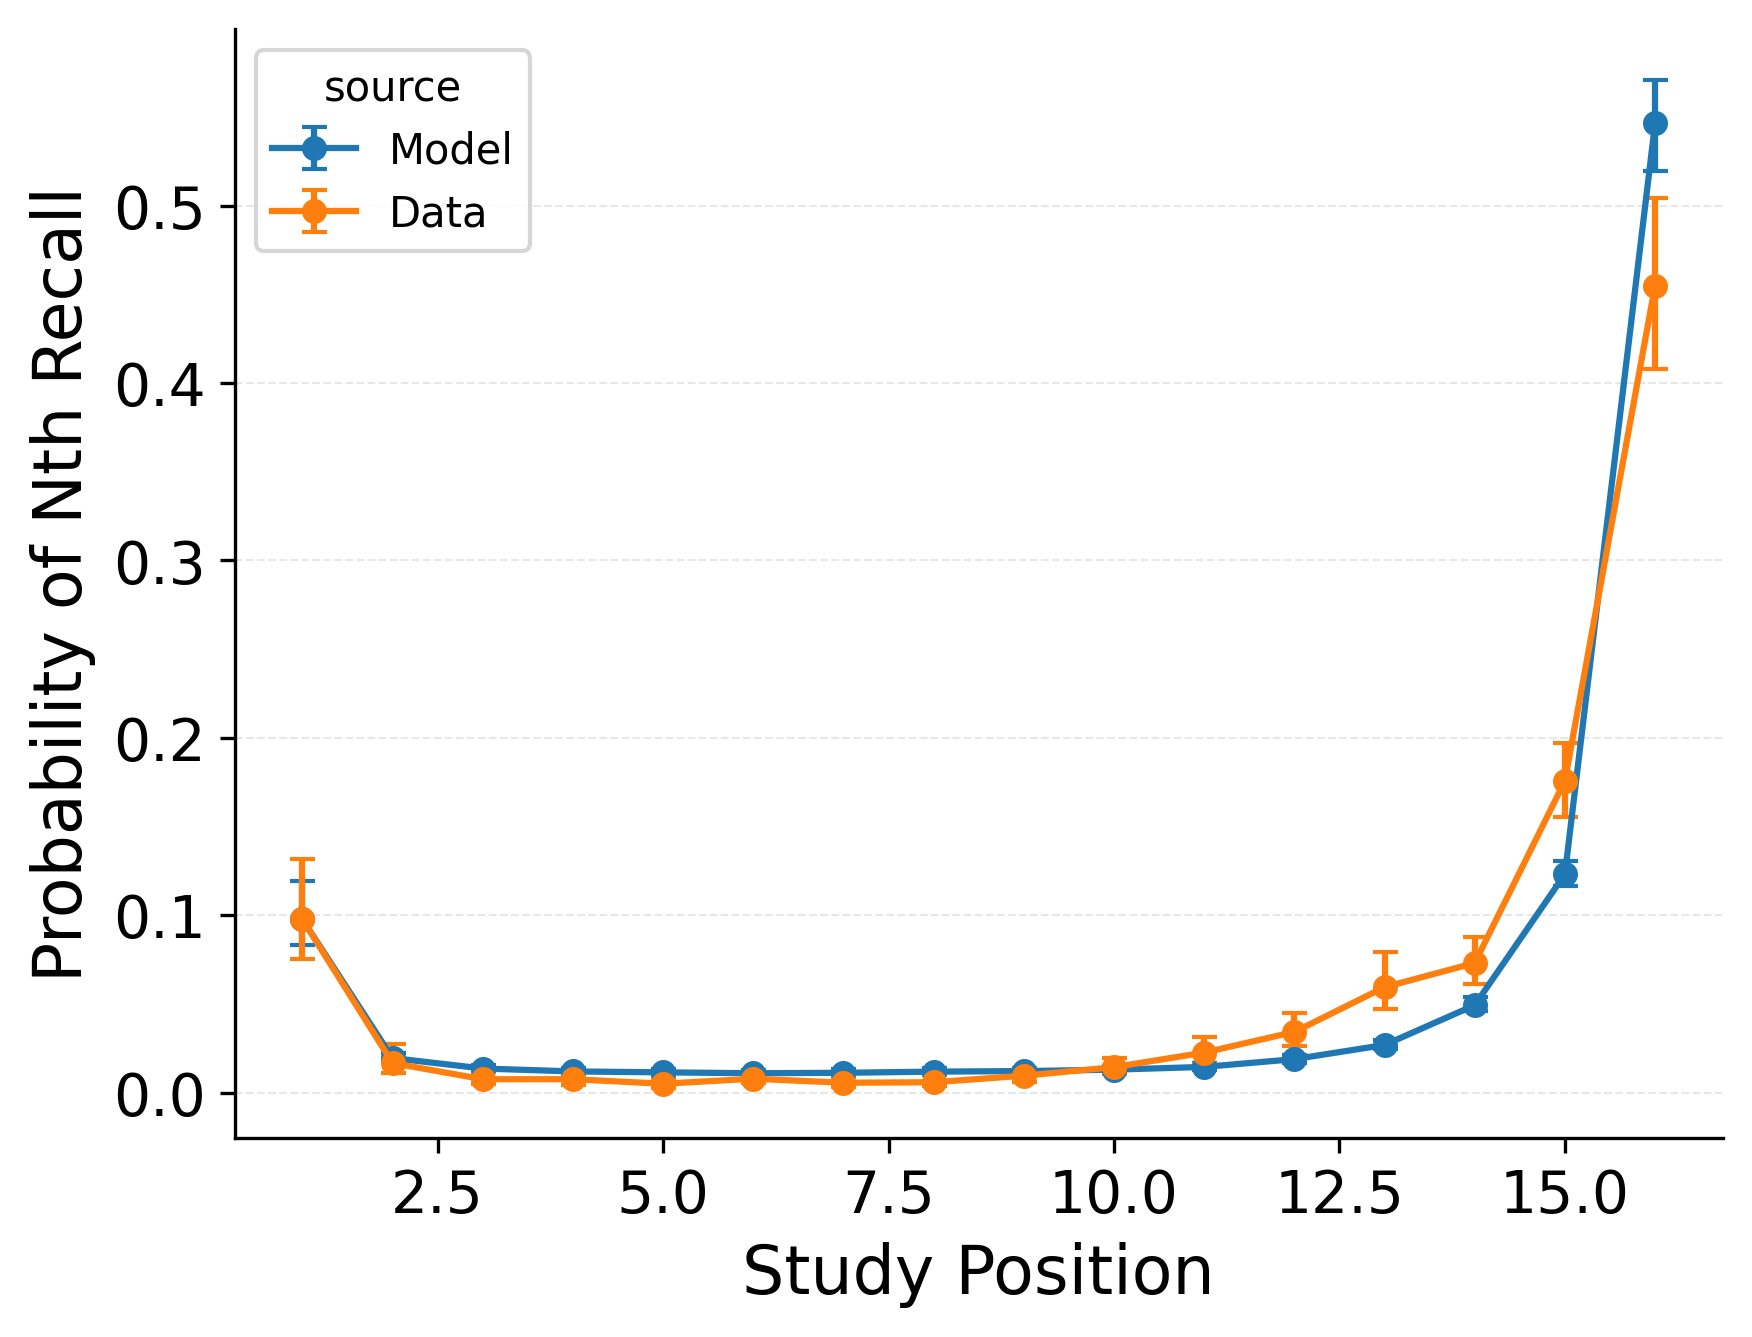
\includegraphics{figures/HealeyKahana2014_CRU_with_Pre-Expt__Primacy__and_StartDrift_Fitting_pnr.png}\end{minipage}%
%
\begin{minipage}{0.33\linewidth}
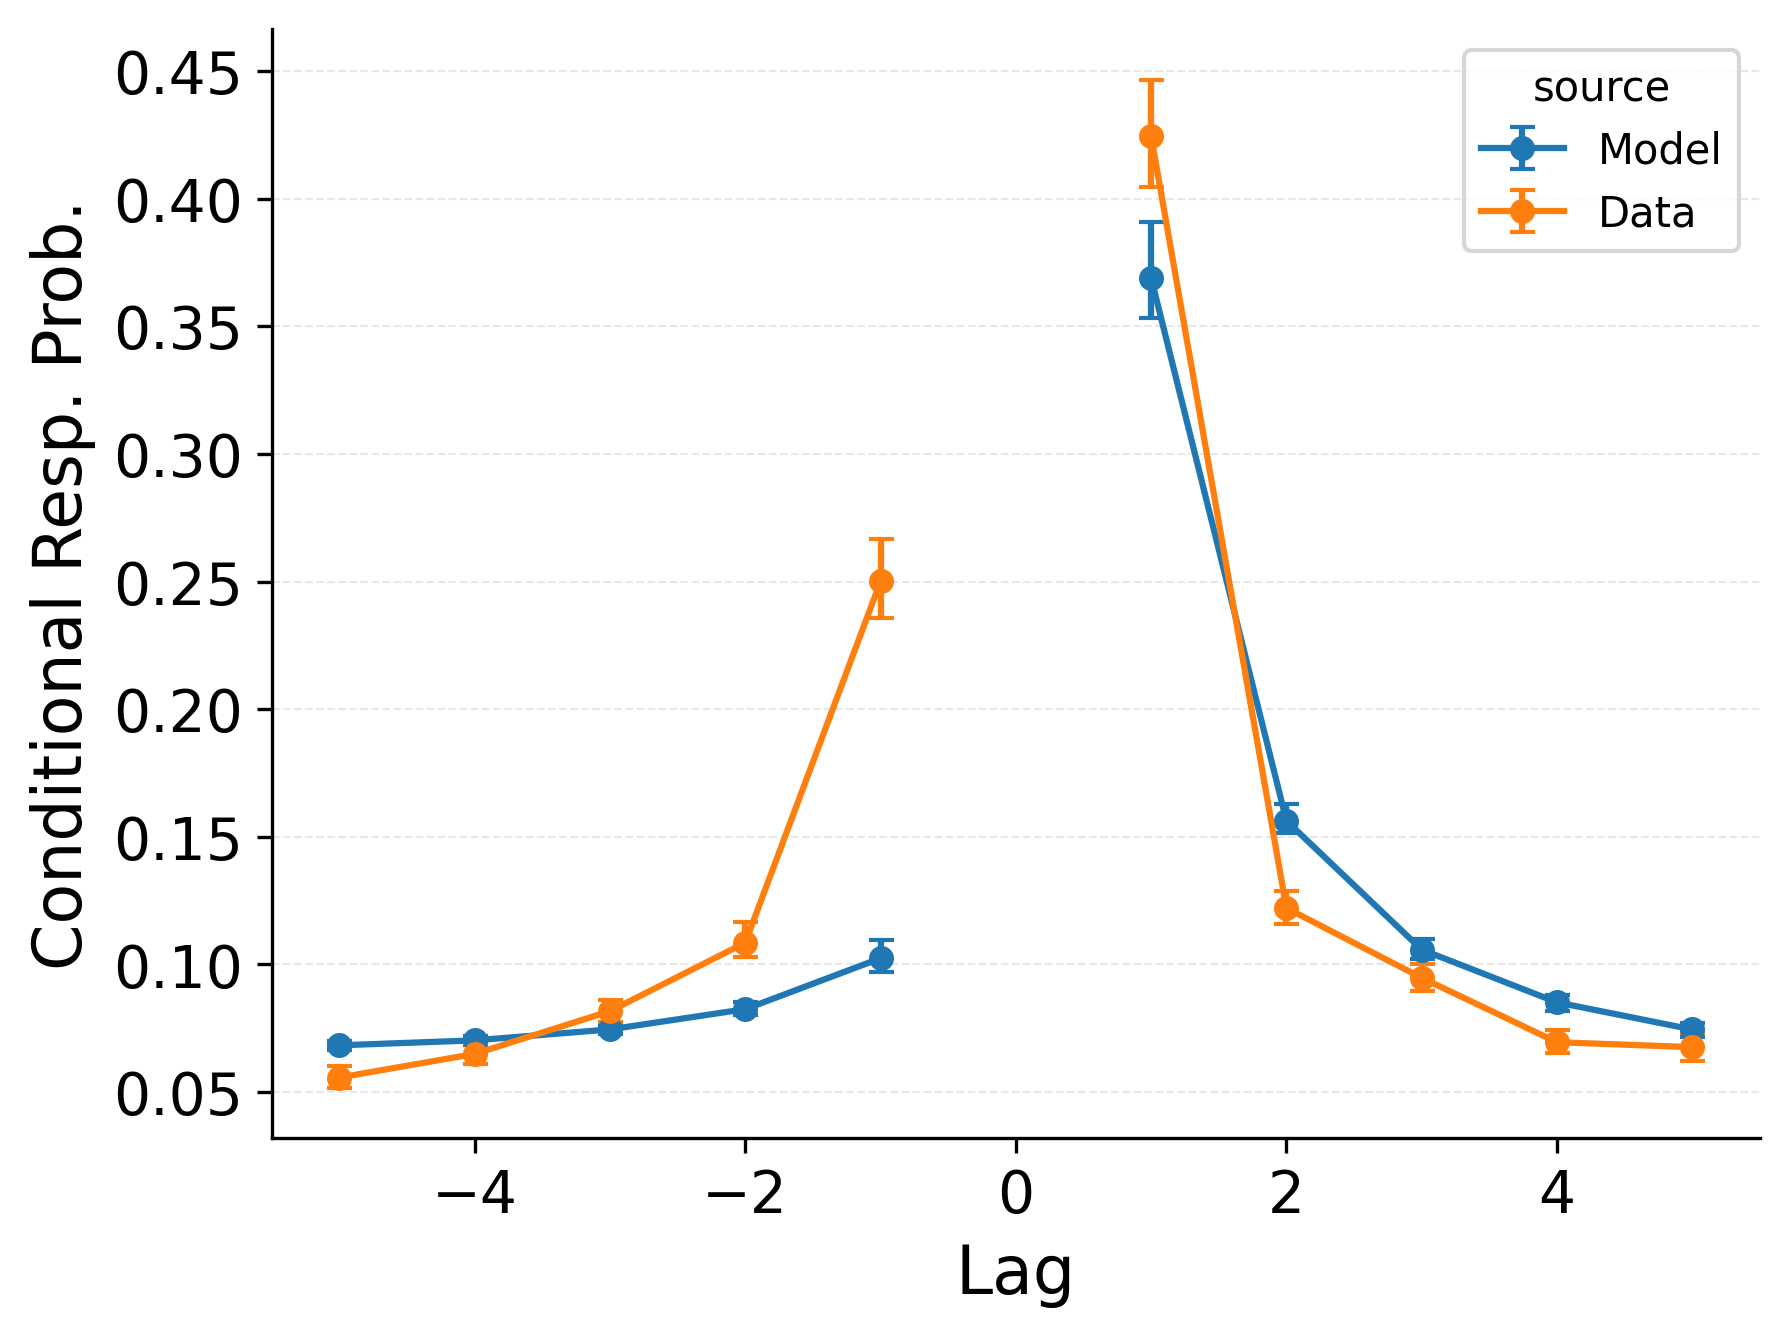
\includegraphics{figures/HealeyKahana2014_CRU_with_Pre-Expt__Primacy__and_StartDrift_Fitting_crp.png}\end{minipage}%
%
\begin{minipage}{0.33\linewidth}
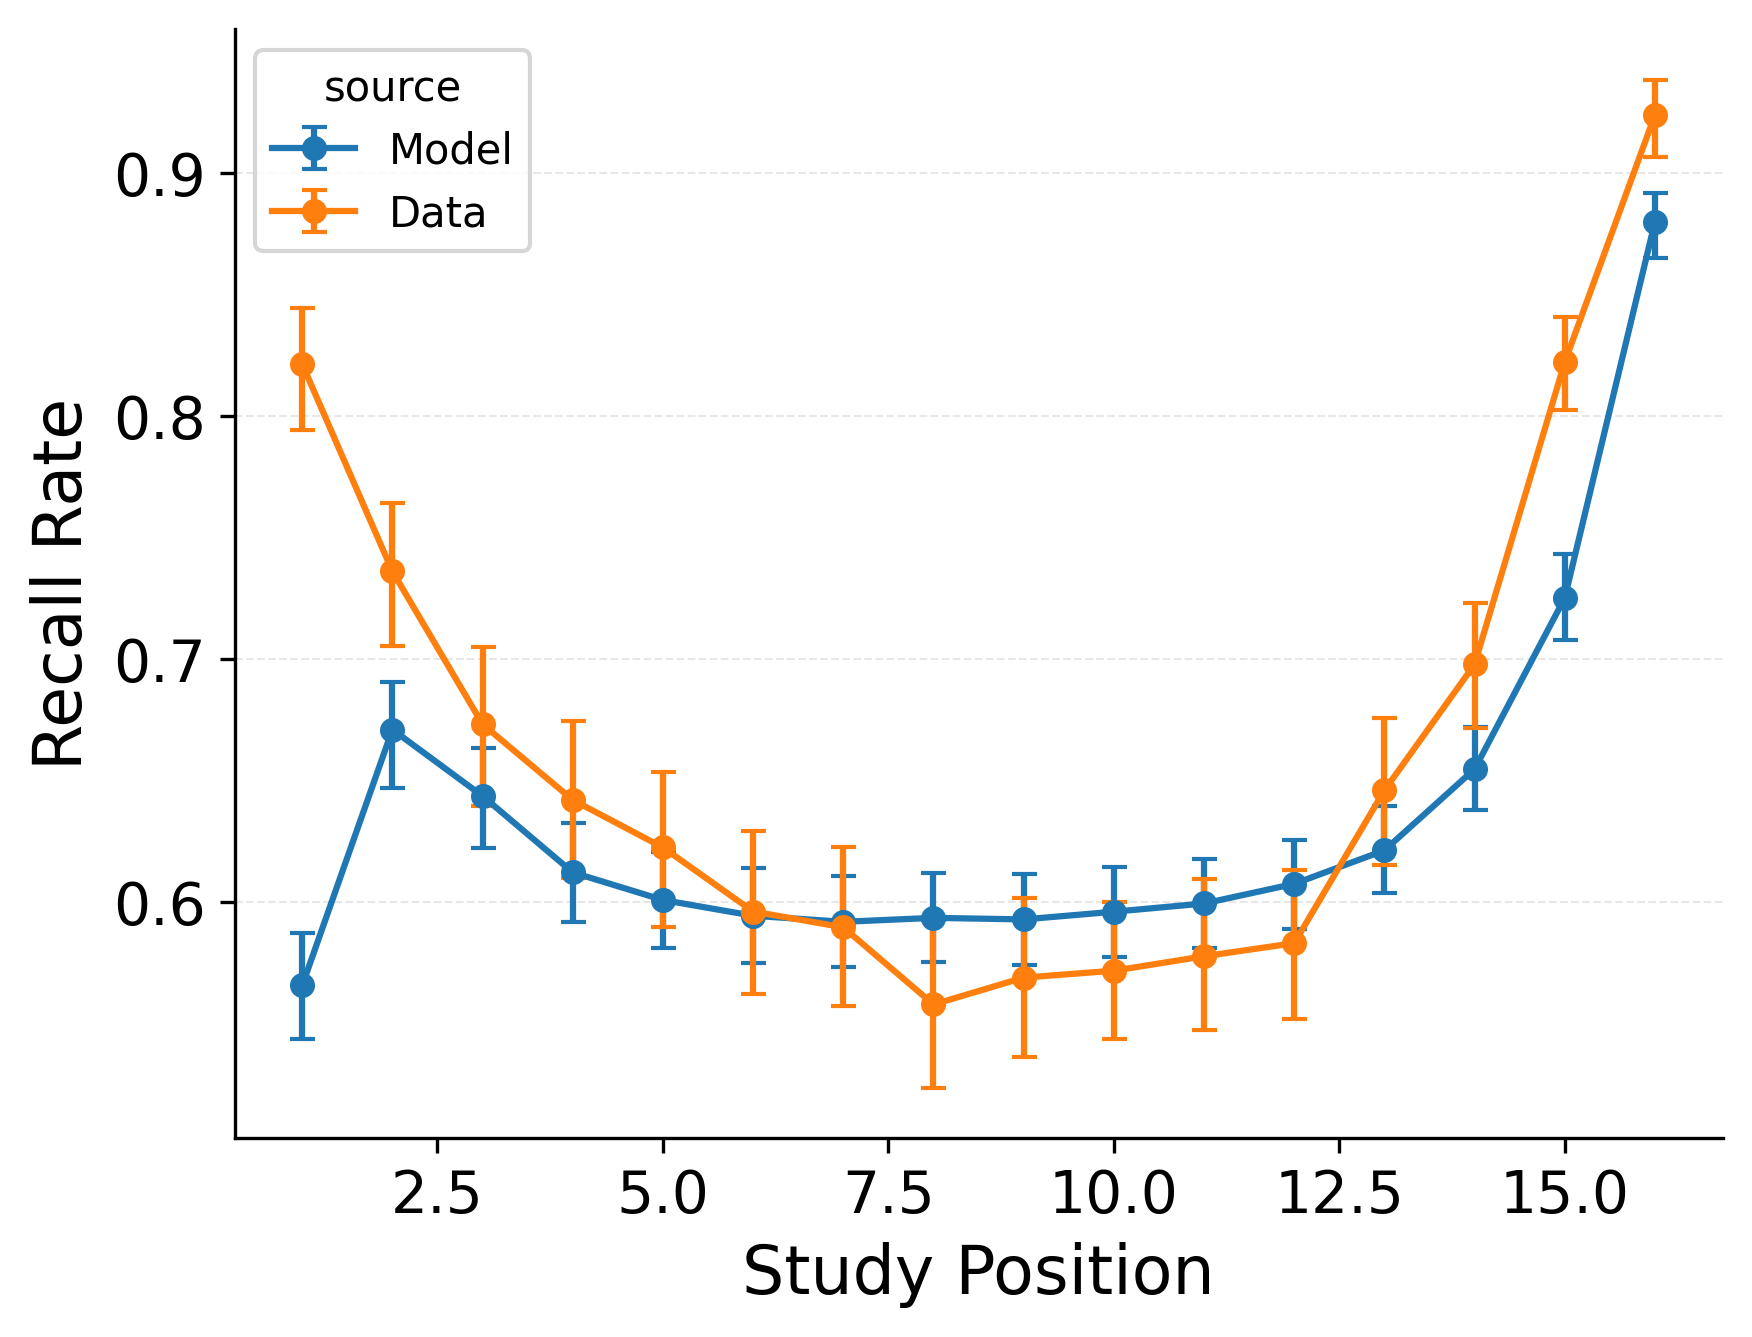
\includegraphics{figures/HealeyKahana2014_CRU_with_Pre-Expt__Primacy__and_StartDrift_Fitting_spc.png}\end{minipage}%
\newline
\begin{minipage}{0.33\linewidth}
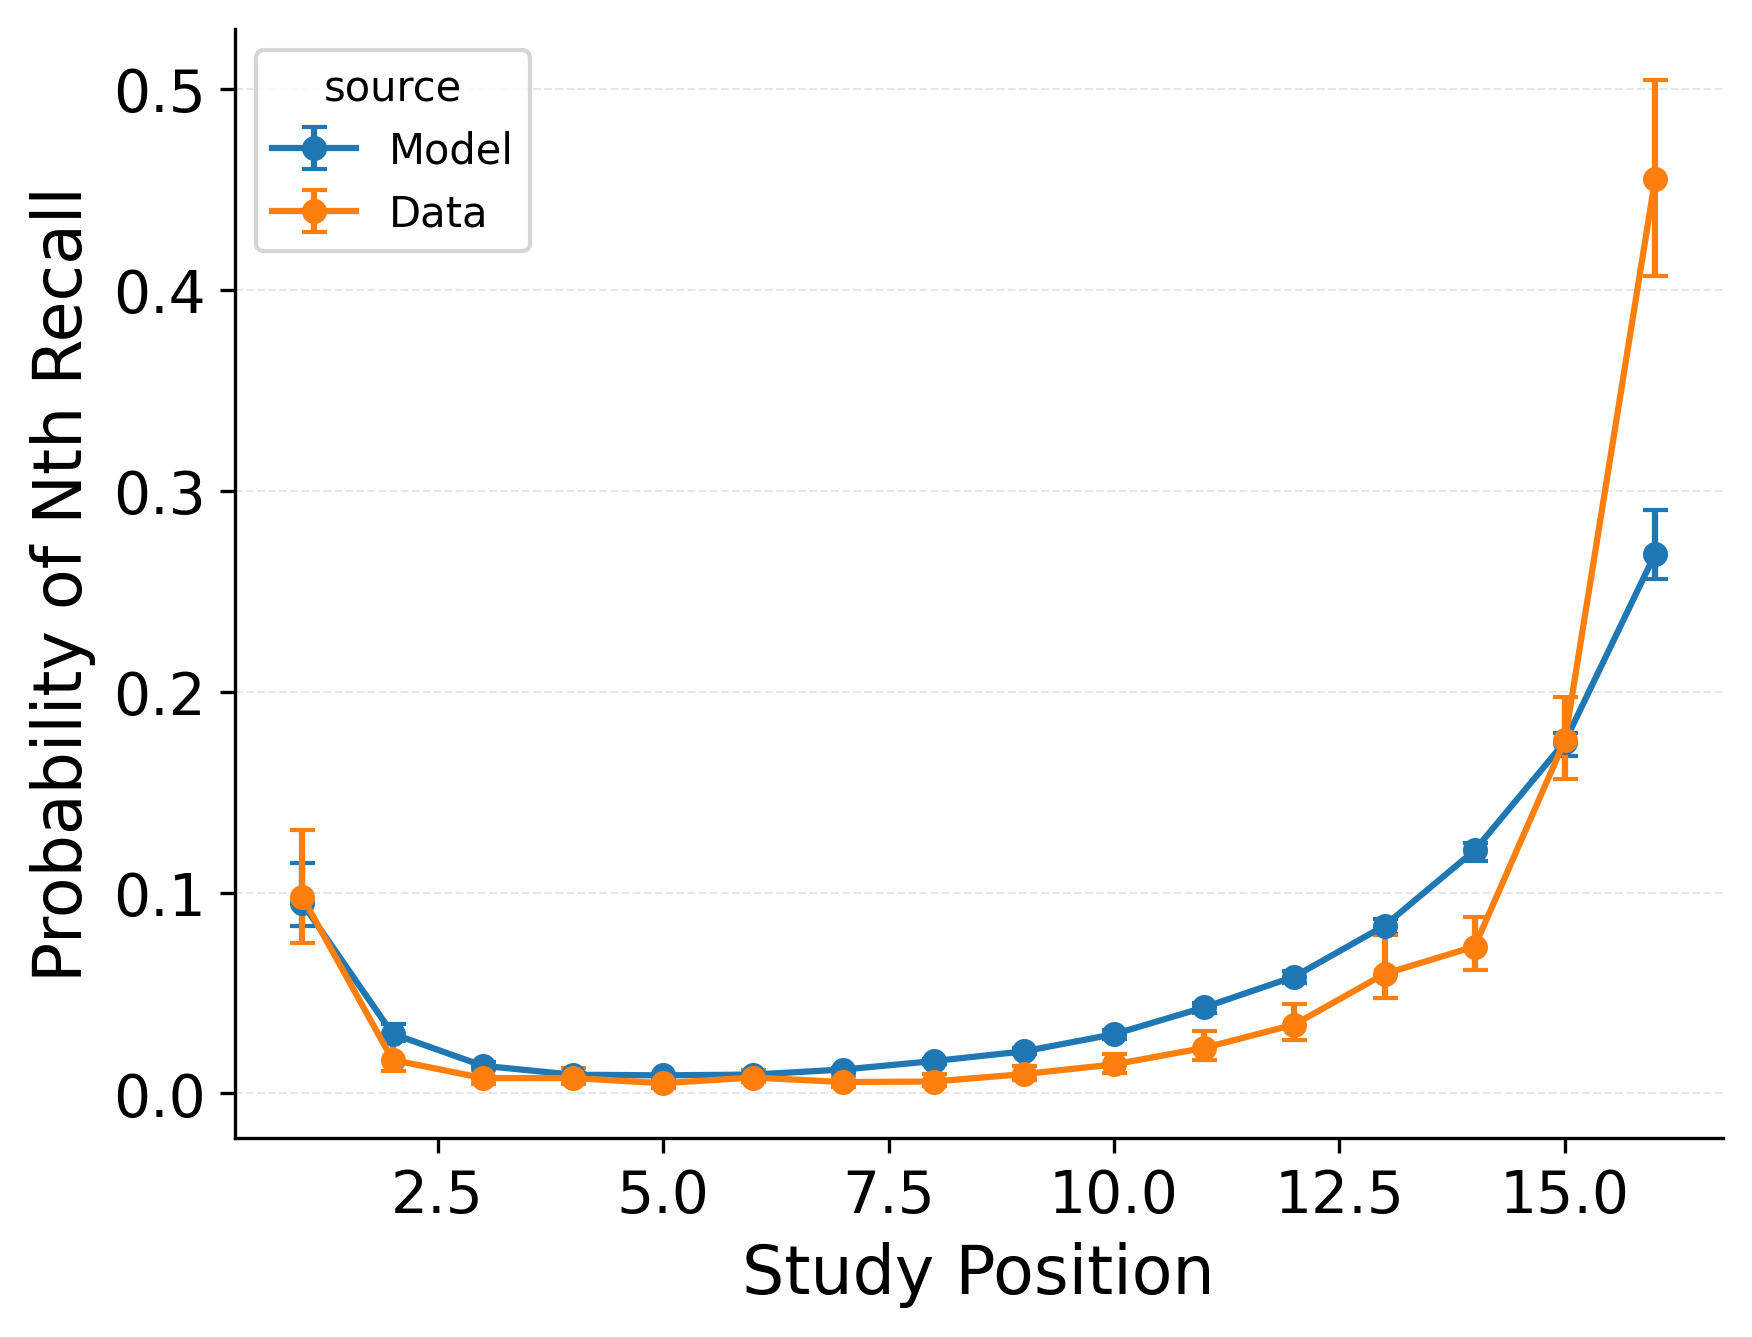
\includegraphics{figures/HealeyKahana2014_CRU_with_Feature-to-Context__Primacy__and_StartDrift_Fitting_pnr.png}\end{minipage}%
%
\begin{minipage}{0.33\linewidth}
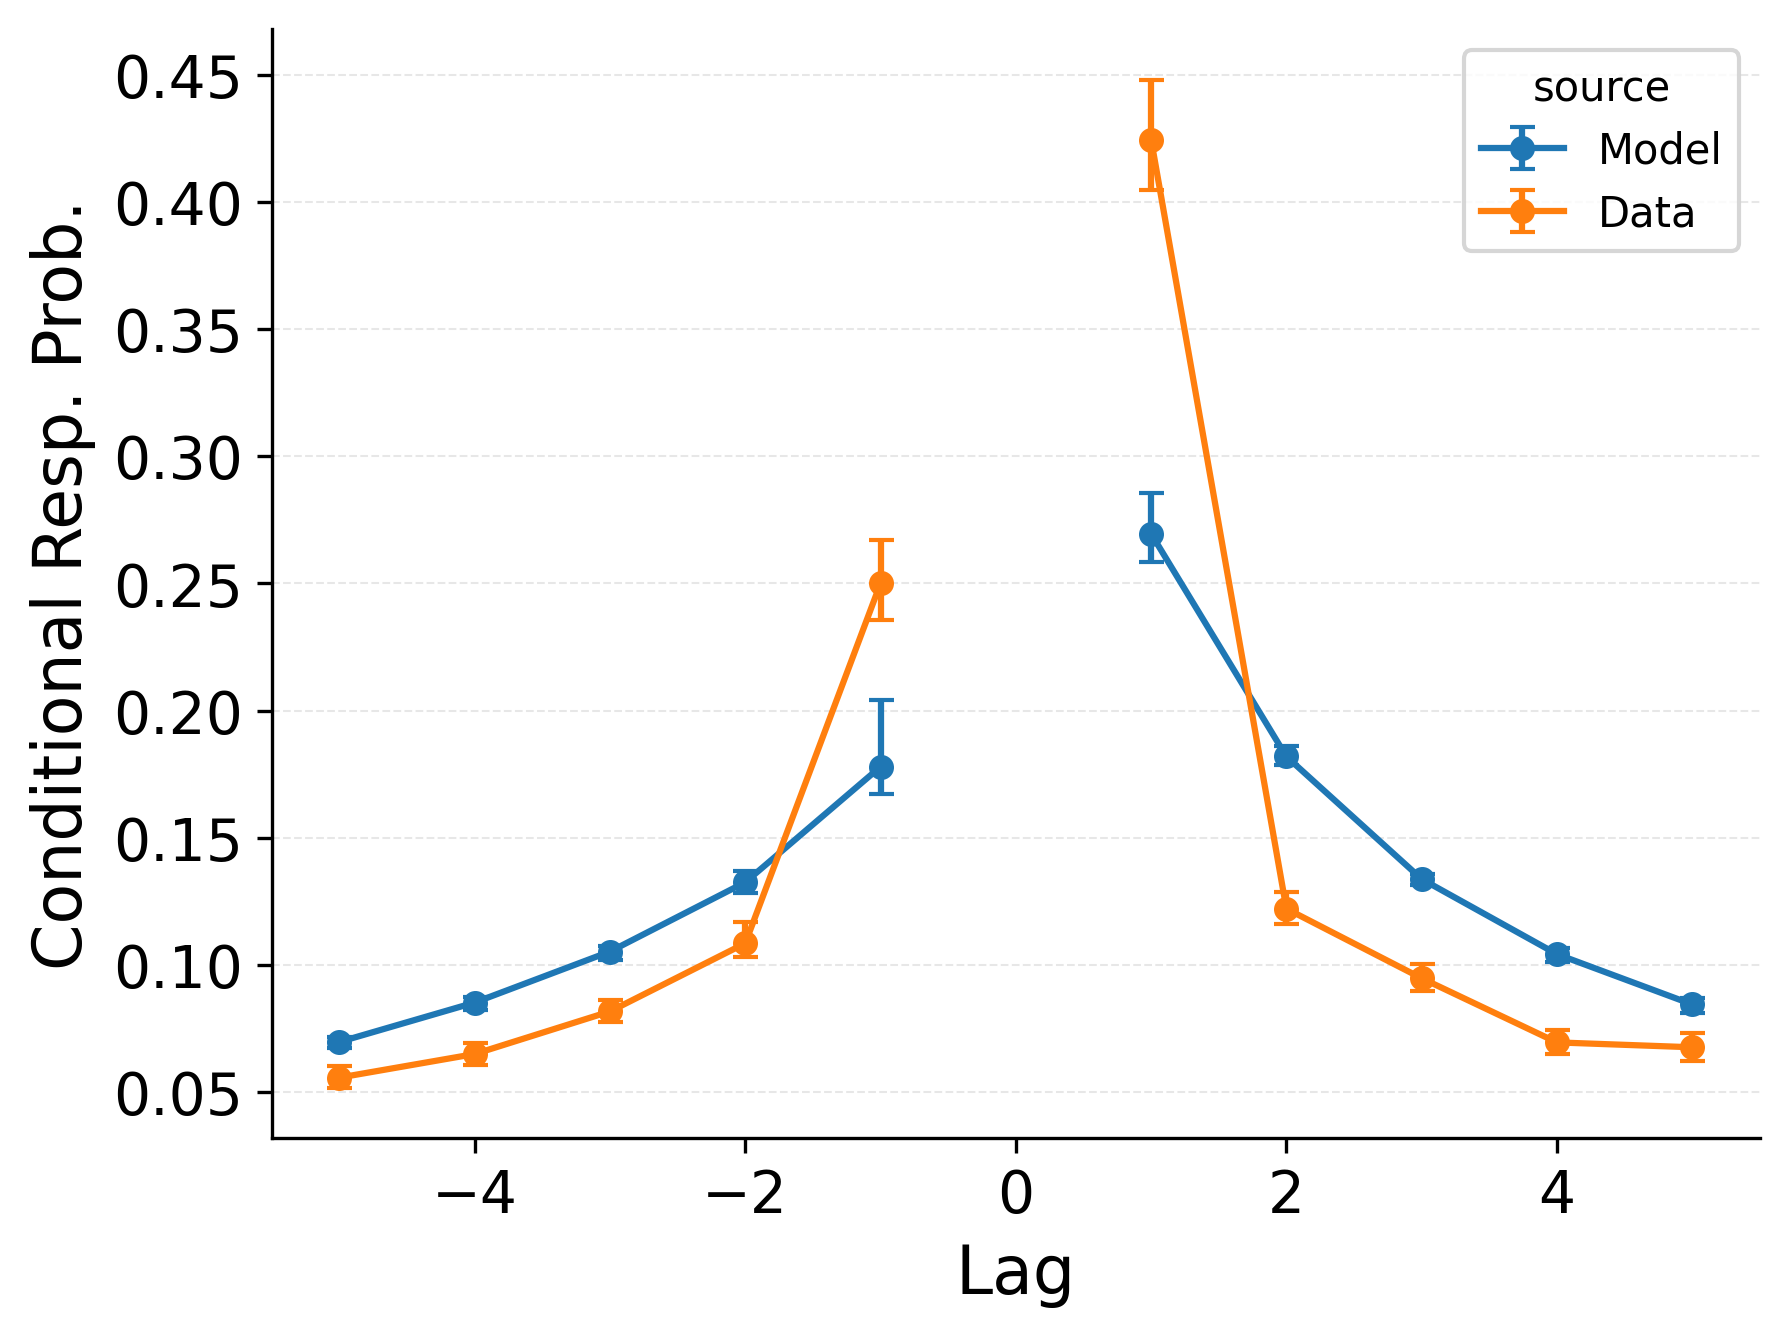
\includegraphics{figures/HealeyKahana2014_CRU_with_Feature-to-Context__Primacy__and_StartDrift_Fitting_crp.png}\end{minipage}%
%
\begin{minipage}{0.33\linewidth}
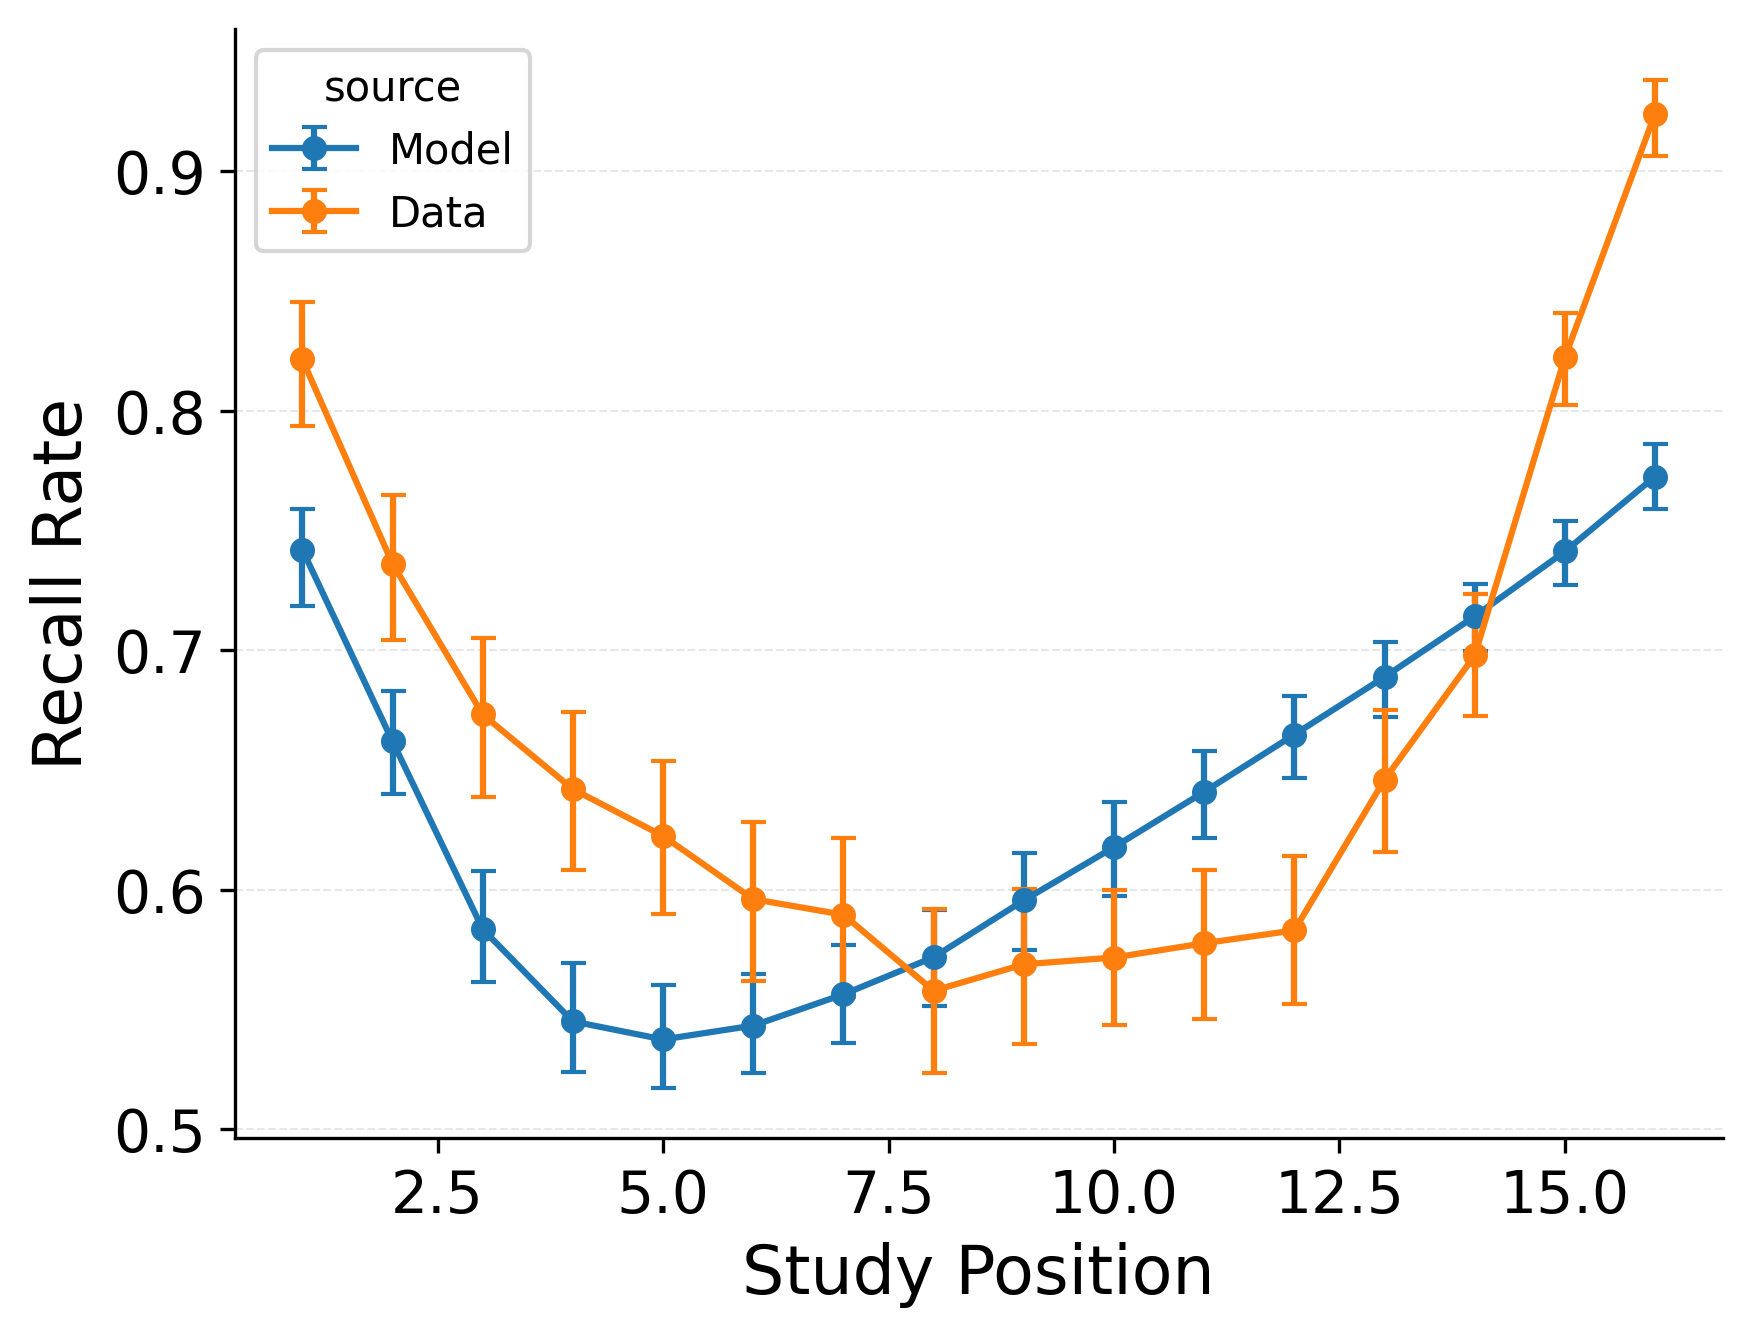
\includegraphics{figures/HealeyKahana2014_CRU_with_Feature-to-Context__Primacy__and_StartDrift_Fitting_spc.png}\end{minipage}%
\newline
\begin{minipage}{0.33\linewidth}
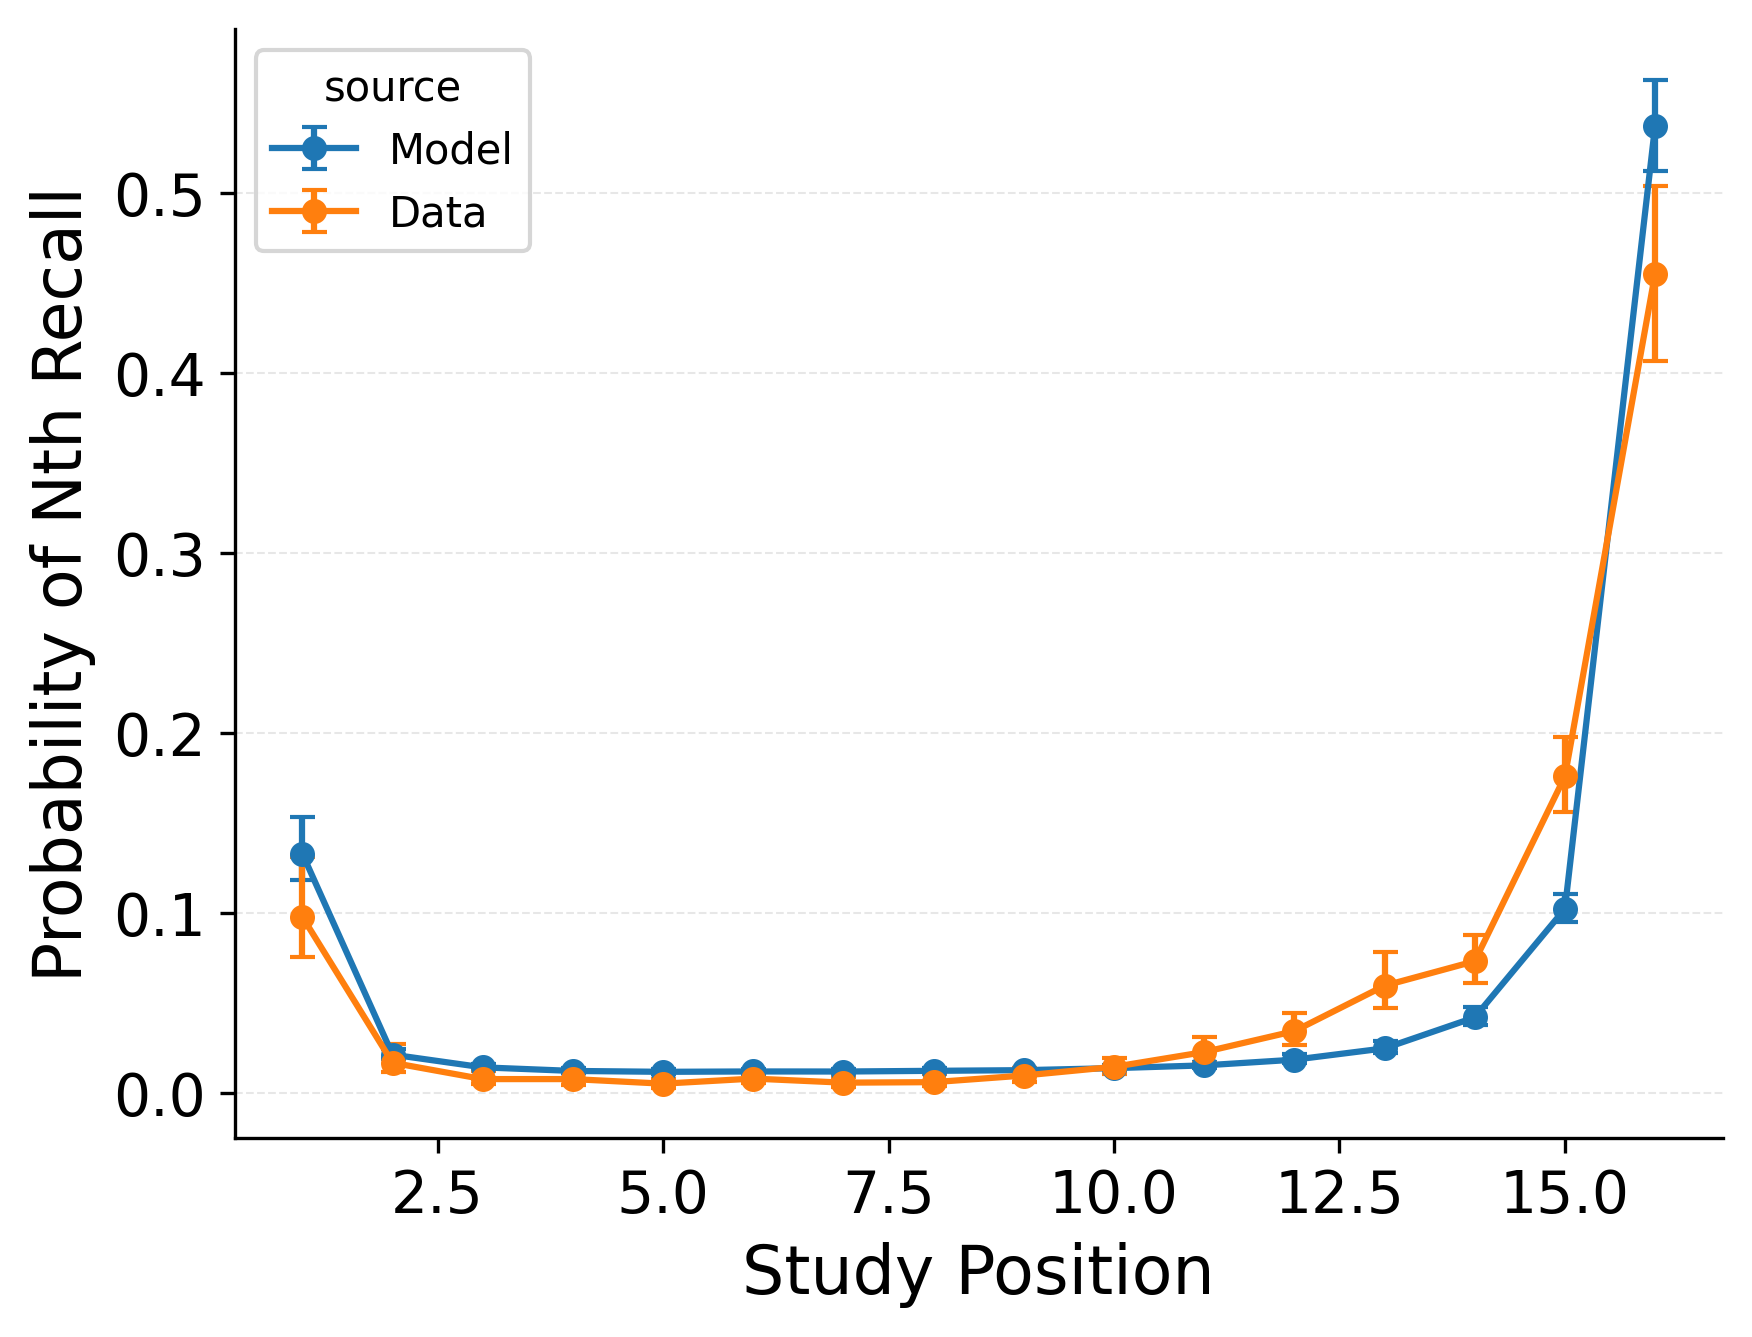
\includegraphics{figures/HealeyKahana2014_CRU_with_Feature-to-Context__Pre-Expt__Primacy__and_StartDrift_Fitting_pnr.png}\end{minipage}%
%
\begin{minipage}{0.33\linewidth}
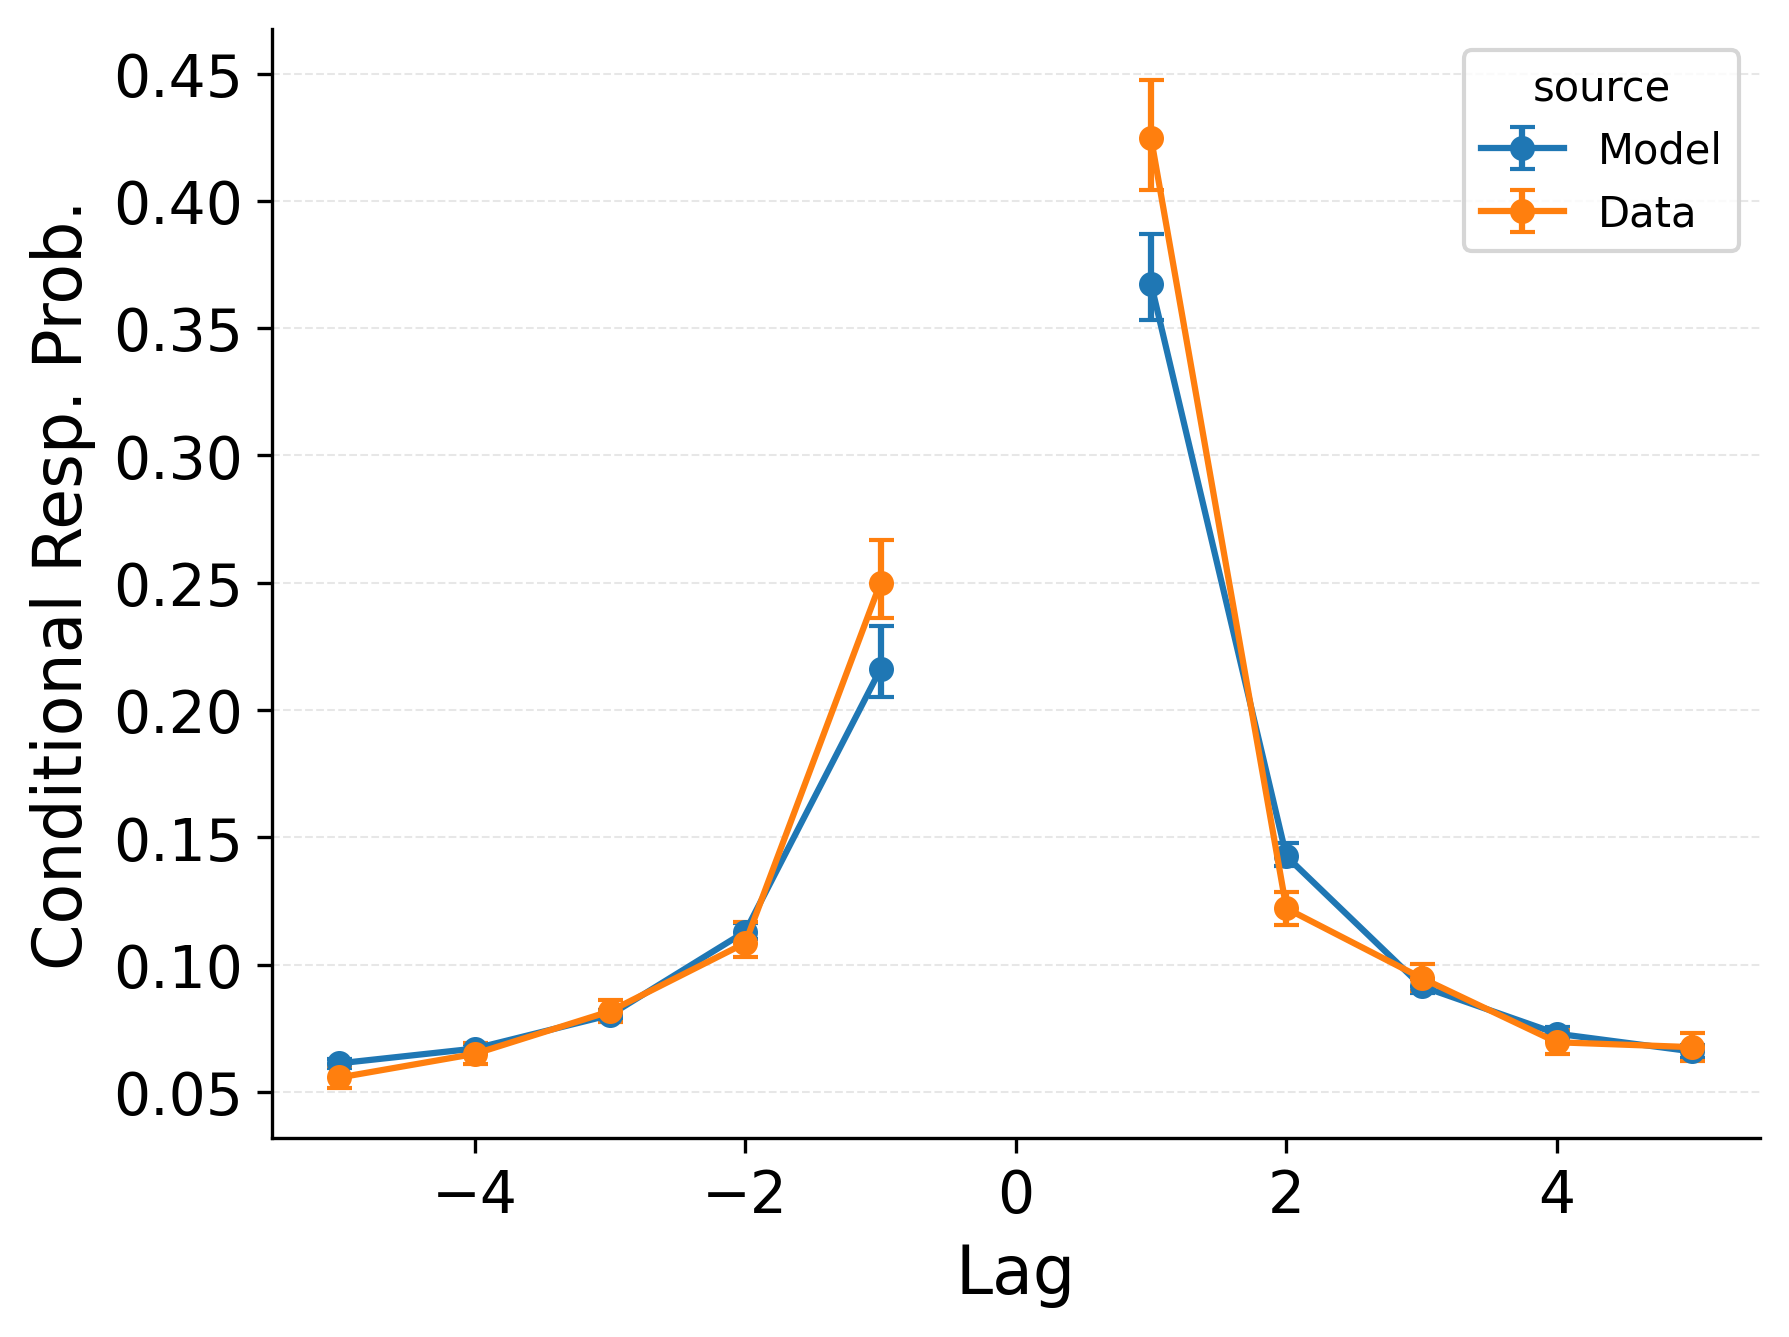
\includegraphics{figures/HealeyKahana2014_CRU_with_Feature-to-Context__Pre-Expt__Primacy__and_StartDrift_Fitting_crp.png}\end{minipage}%
%
\begin{minipage}{0.33\linewidth}
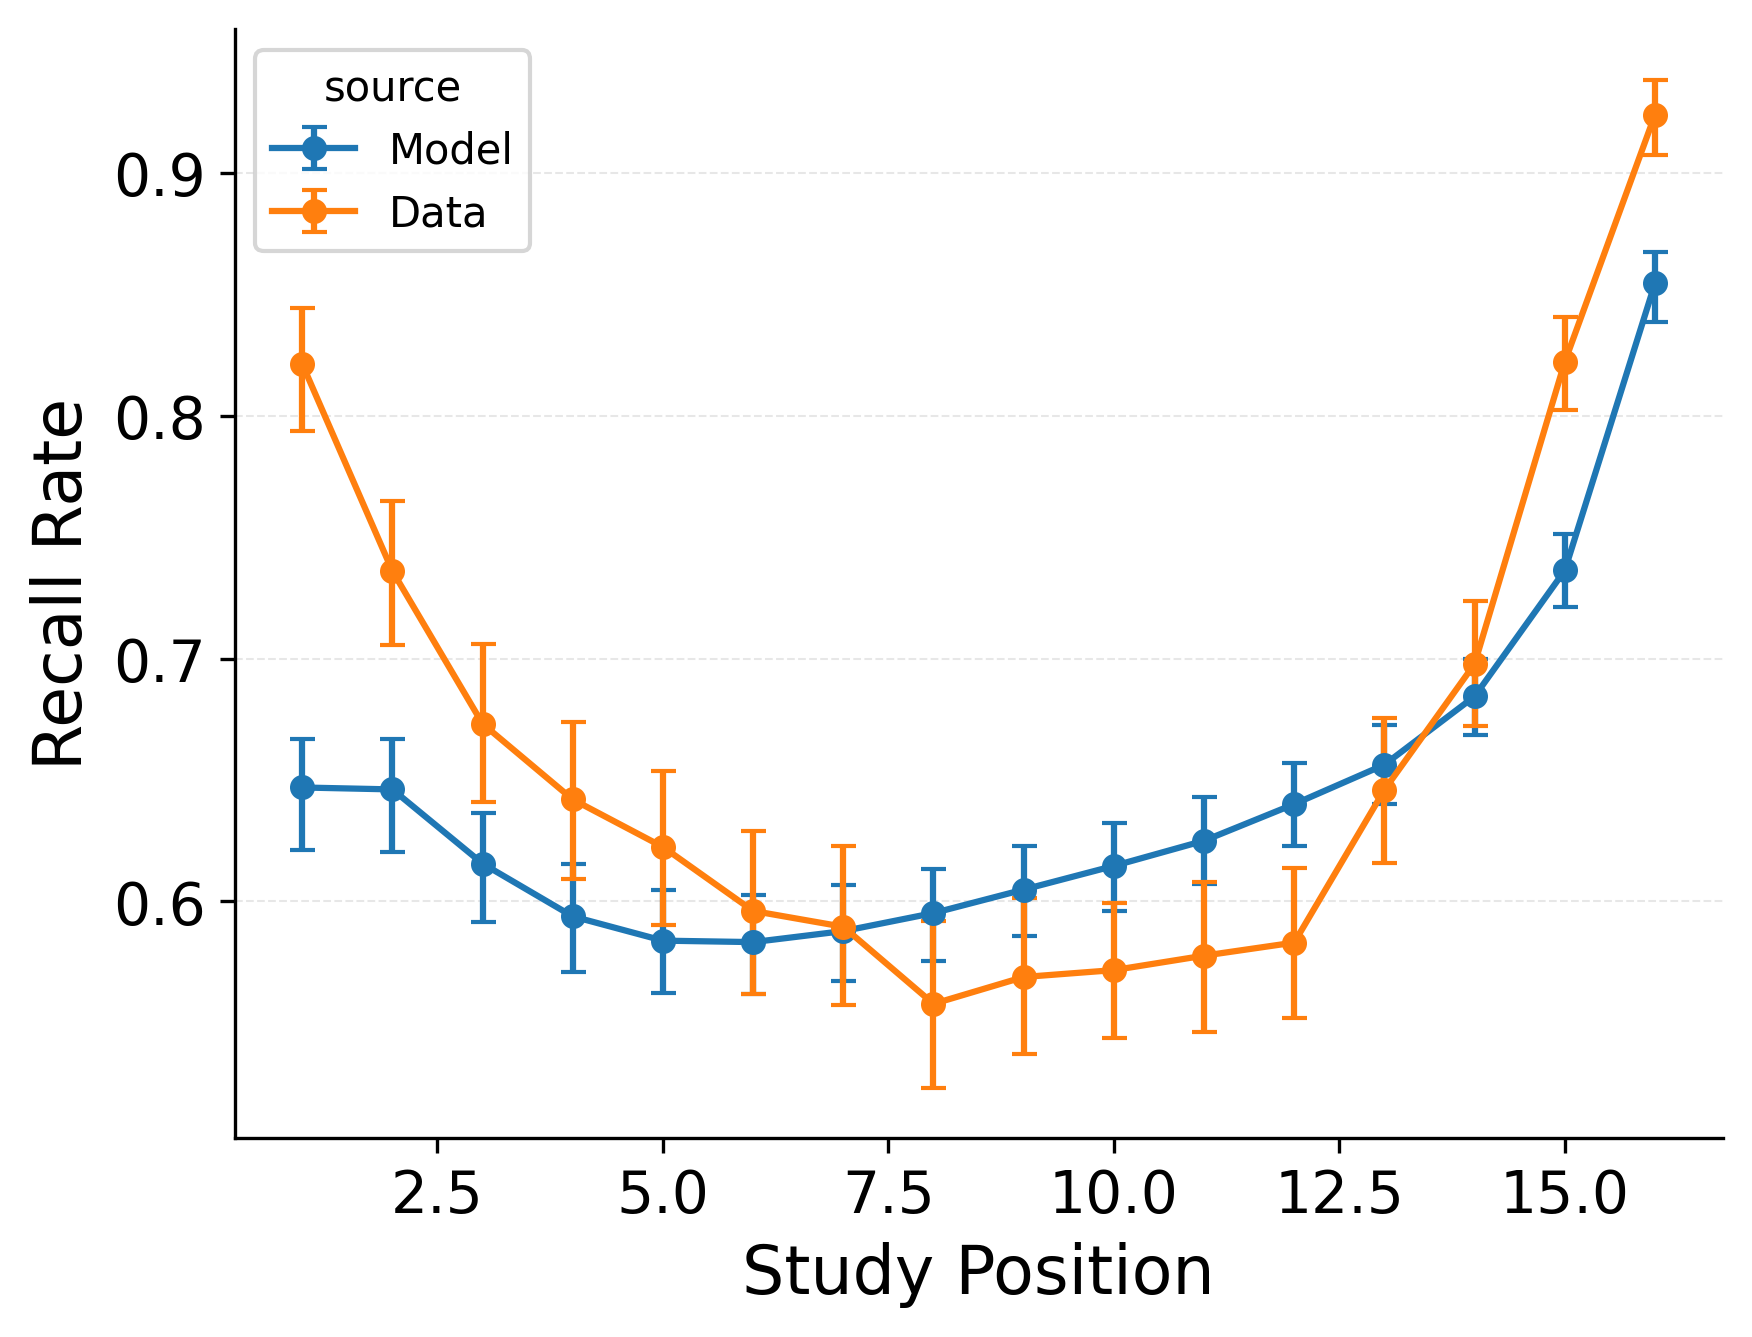
\includegraphics{figures/HealeyKahana2014_CRU_with_Feature-to-Context__Pre-Expt__Primacy__and_StartDrift_Fitting_spc.png}\end{minipage}%

\end{figure}%

In free recall, the lag-contiguity effect is bidirectional and
asymmetric, with participants more likely to transition to items that
were presented immediately after the just-recalled item, but also
sometimes transitioning to items that were presented immediately before
the just-recalled item in the original study list. Standard CRU is able
to simulate a bidirectional lag-contiguity effect, but it substantially
underestimates the strength of the effect compared to the data,
predicting around a 20\% probability of +1 lag transition while the data
shows over a 40\% probability of +1 lag transition. Standard CRU shows a
similar discrepancy for a backward -1 lag transition.

CMR controls the shape of the lag-contiguity effect with a set of
parameters controlling the relative strength of different associative
structures. These parameters include \(\gamma\), which influences
context reinstatement during retrieval, and \(\alpha\) and \(\delta\),
which influence the competition between items during retrieval. For
larger values of the \(\gamma\) parameter, the context associated with a
just-recalled item is more stronglyreinstated during retrieval, helping
capture high rates of short lag backward transitions in the
lag-contiguity effect. Figure~\ref{fig-shiftlearning} (left) shows how
altering \(\gamma\) affects the lag-CRP for CMR, supporting this
interpretation. The simulation was configured similarly to those
described in the previous section, using parameters fit to Healey and
Kahana (\citeproc{ref-healey2014memory}{2014}), and shifting \(\gamma\)
from 0 to .9 in increments of 0.1.

CMR's \(\delta\) and \(\alpha\) parameters provide a pre-experimental
context-to-feature memory that can influence the lag-contiguity effect
by tuning the strength of associations from context representations to
item representations. When \(\delta\) is much higher than \(\alpha\),
the lag-contiguity effect is facilitated by favoring neighbors of the
just-recalled item in the competition between items during retrieval.
Alternatively, setting \(\delta\) to match \(\alpha\) or to zero can
flatten the lag-contiguity effect by making all items equally likely to
be activated by a context feature associated with a just-recalled item.
When \(\gamma\) is configured to 0 -- as it effectively is in CRU --
tuning \(\delta\) no longer influences rates of backward transitions in
the lag-contiguity effect, as the experimental associations that would
facilitate these backward transitions are no longer present.
Figure~\ref{fig-shiftlearning} (right) illustrates the impact of
shifting \(\delta\) on the shape of the lag-CRP for CMR when \(\gamma\)
is not set to 0. The simulation was configured similarly to the previous
section, using parameters fit to Healey and Kahana
(\citeproc{ref-healey2014memory}{2014}), and shifting \(\delta\) from 0
to 8.9 in increments of 1. When \(\gamma\) is configured to non-zero
values, higher values of \(\delta\) can simultaneously drive both
forward and backward transitions in the lag-contiguity effect, reducing
the rate of more distant transitions while increasing the rate of closer
transitions.

Freeing \(\gamma\), \(\delta\), and \(\alpha\) in CMR allows the model
to flexibly capture the strength and asymmetry of the lag-contiguity
effect. Figure~\ref{fig-fitlagcrp} (Row 2) illustrates CRU's performance
when extended to include CMR's dynamic feature-to-context memory
(\(\gamma\)) alongside primacy and recency mechanisms
(\(\phi_\text{s}\), \(\phi_\text{d}\), and \(\beta_\text{start}\)).
Simulated summary statistics confirm that this extension allows the
model to better capture the lag-contiguity effect, but the model still
underestimates its overall strength compared to the data. This produces
correspondingly worse performance capturing primacy and recency
benchmarks.

Finally, in the third row of Figure~\ref{fig-fitlagcrp}, extending CRU
to include both CMR's dynamic feature-to-context memory (\(\gamma\)) and
pre-experimental context-to-feature memory (\(\delta\) and \(\alpha\))
alongside established primacy and recency mechanisms allows the model to
better capture all components of the lag-contiguity effect and other
benchmarks. However, this model is exactly CMR: CRU with all of CMR's
mechanisms enabled. This suggests that standard CRU's streamlined
implementation is not sufficient to capture the full range of free
recall phenomena, and underlines that all of CMR's mechanisms are useful
for capturing free recall data, despite the complexity they introduce.

\begin{figure}

\caption{\label{fig-shiftlearning}Simulation of the impact of shifting
CMR's \(\gamma\) (\textbf{Left}) and \(\delta\) (\textbf{Right})
parameters on the conditional response probability as a function of lag
for CMR. Using parameters fit to Healey and Kahana
(\citeproc{ref-healey2014memory}{2014}), the learning rate parameter
\(\gamma\) is shifted from 0 to 1 in increments of 0.1, and the item
support parameter \(\delta\) is shifted from 0 to 10 in increments of 1,
with the color of the lines indicating the value of the parameter.}

\begin{minipage}{0.50\linewidth}
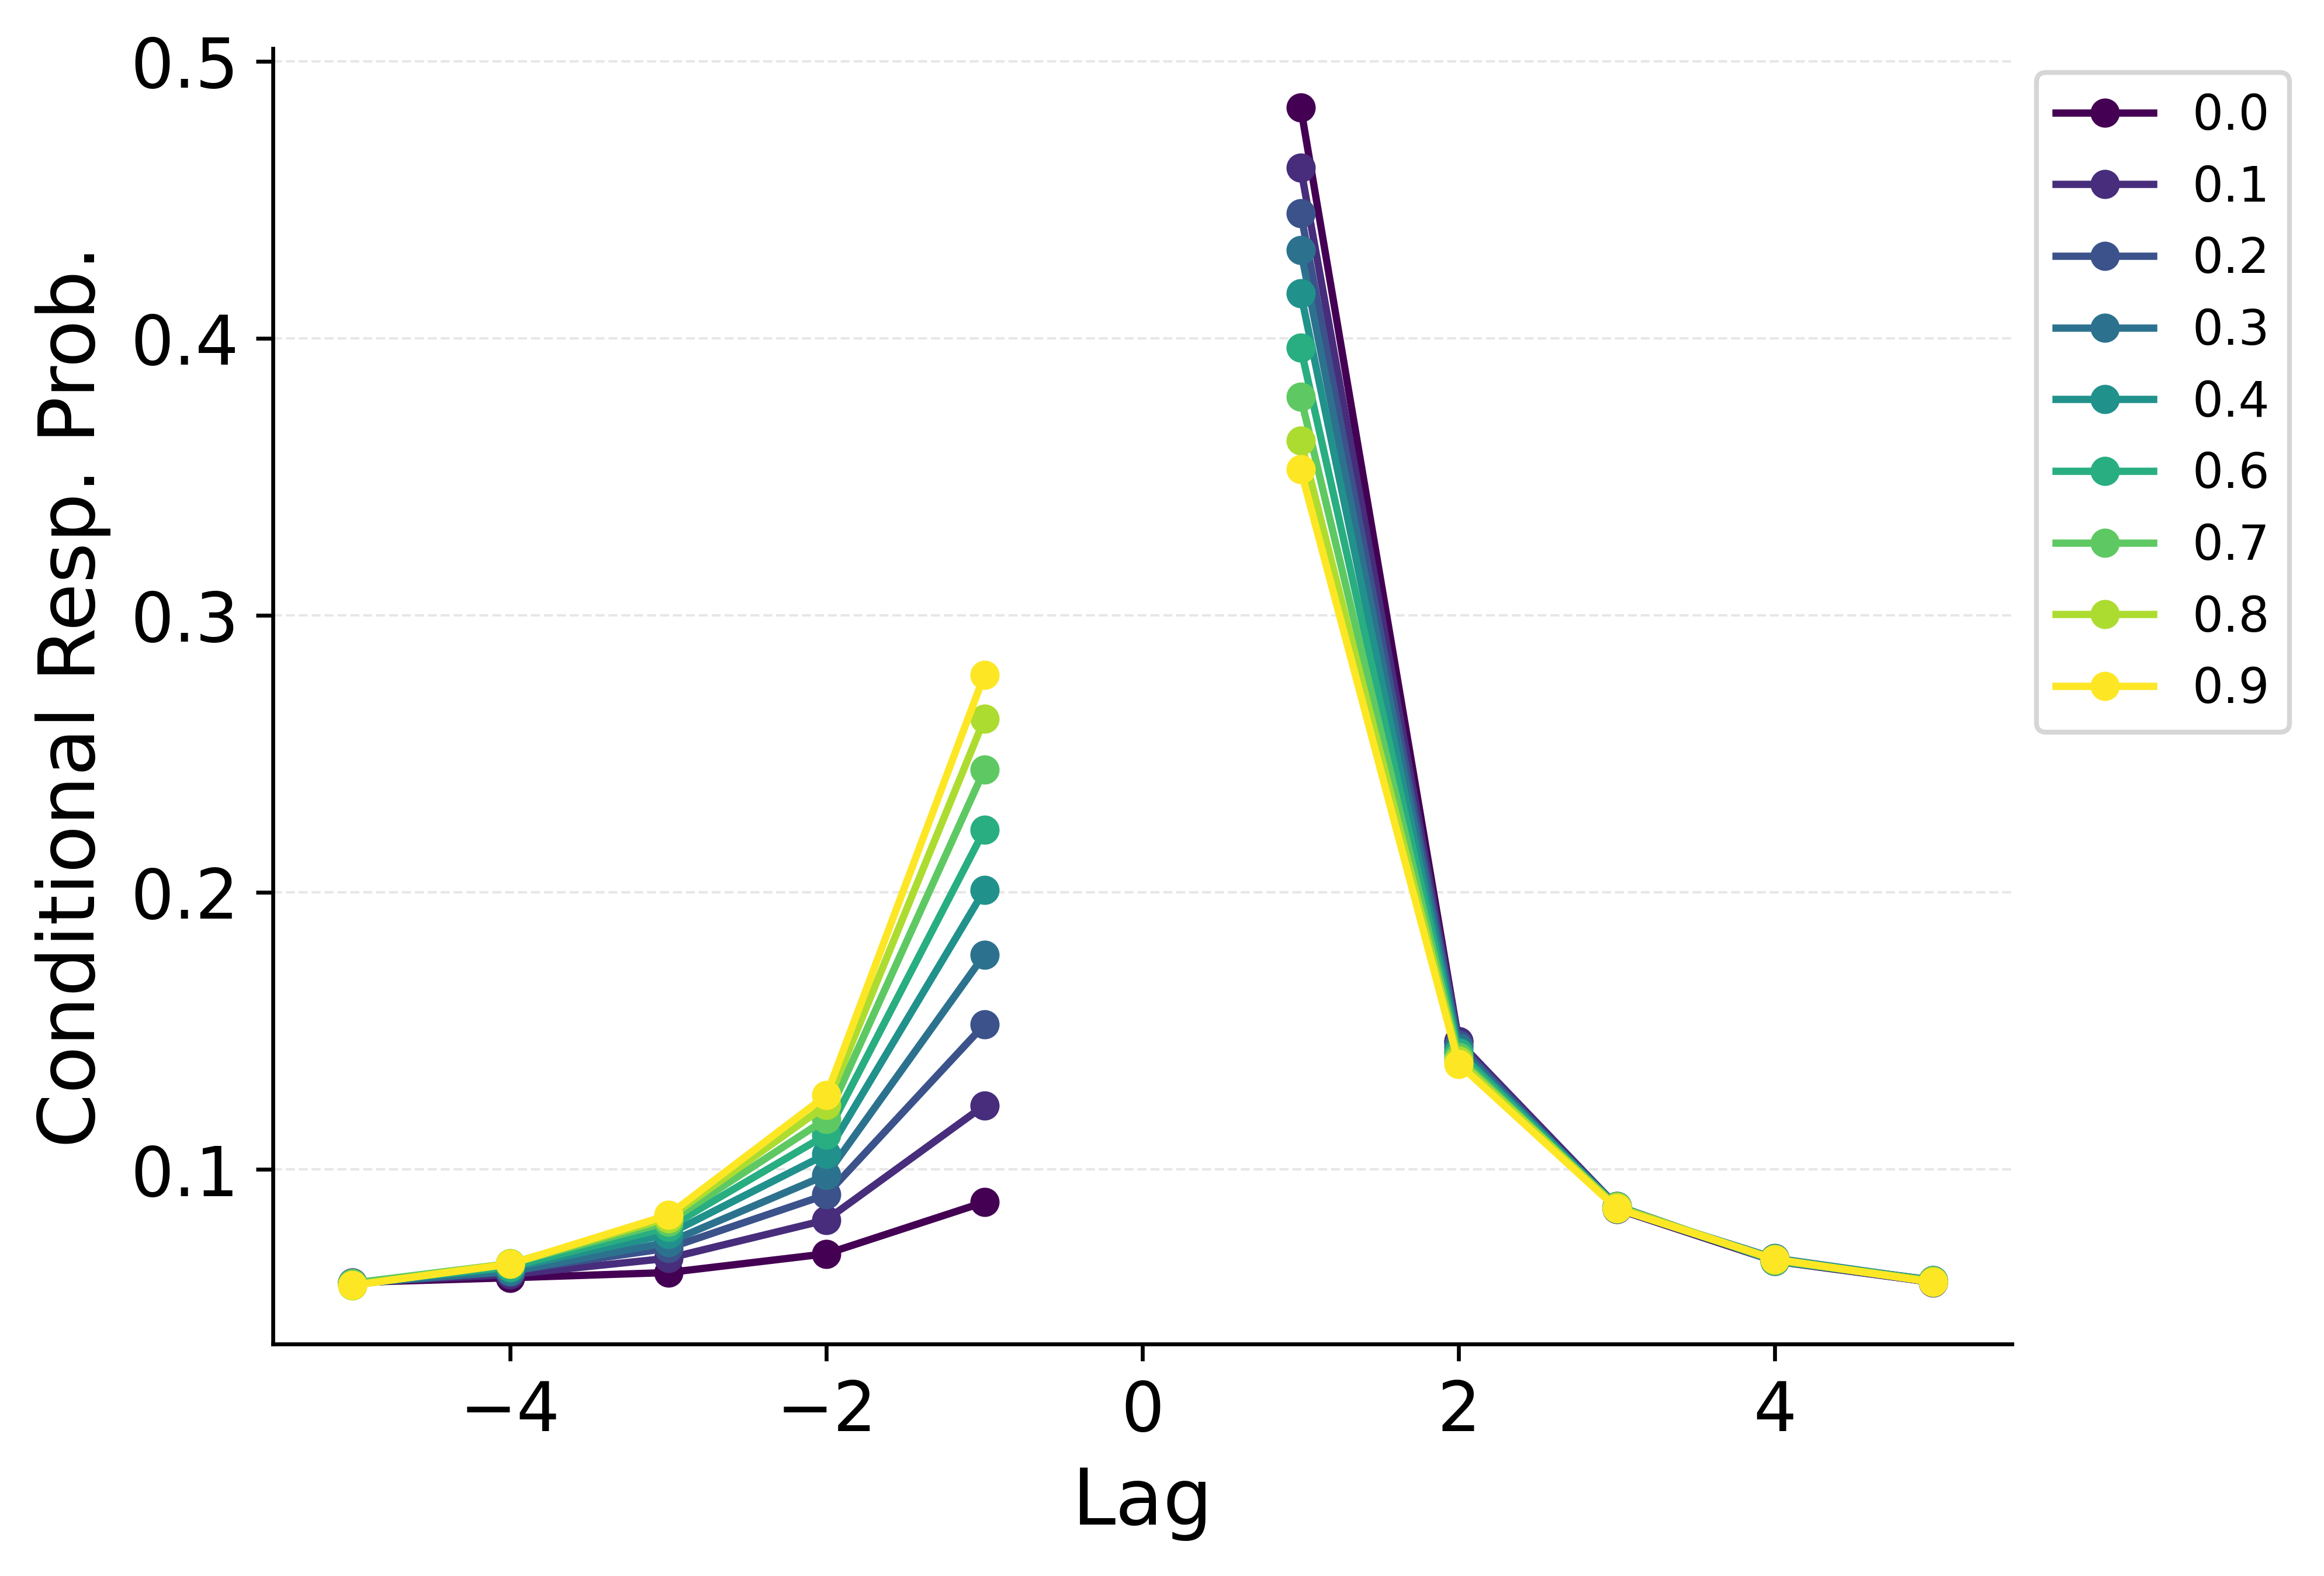
\includegraphics{shifting/BaseCMR_Learning_Rate_Parameter_Shifting_crp_HealeyKahana2014.png}\end{minipage}%
%
\begin{minipage}{0.50\linewidth}
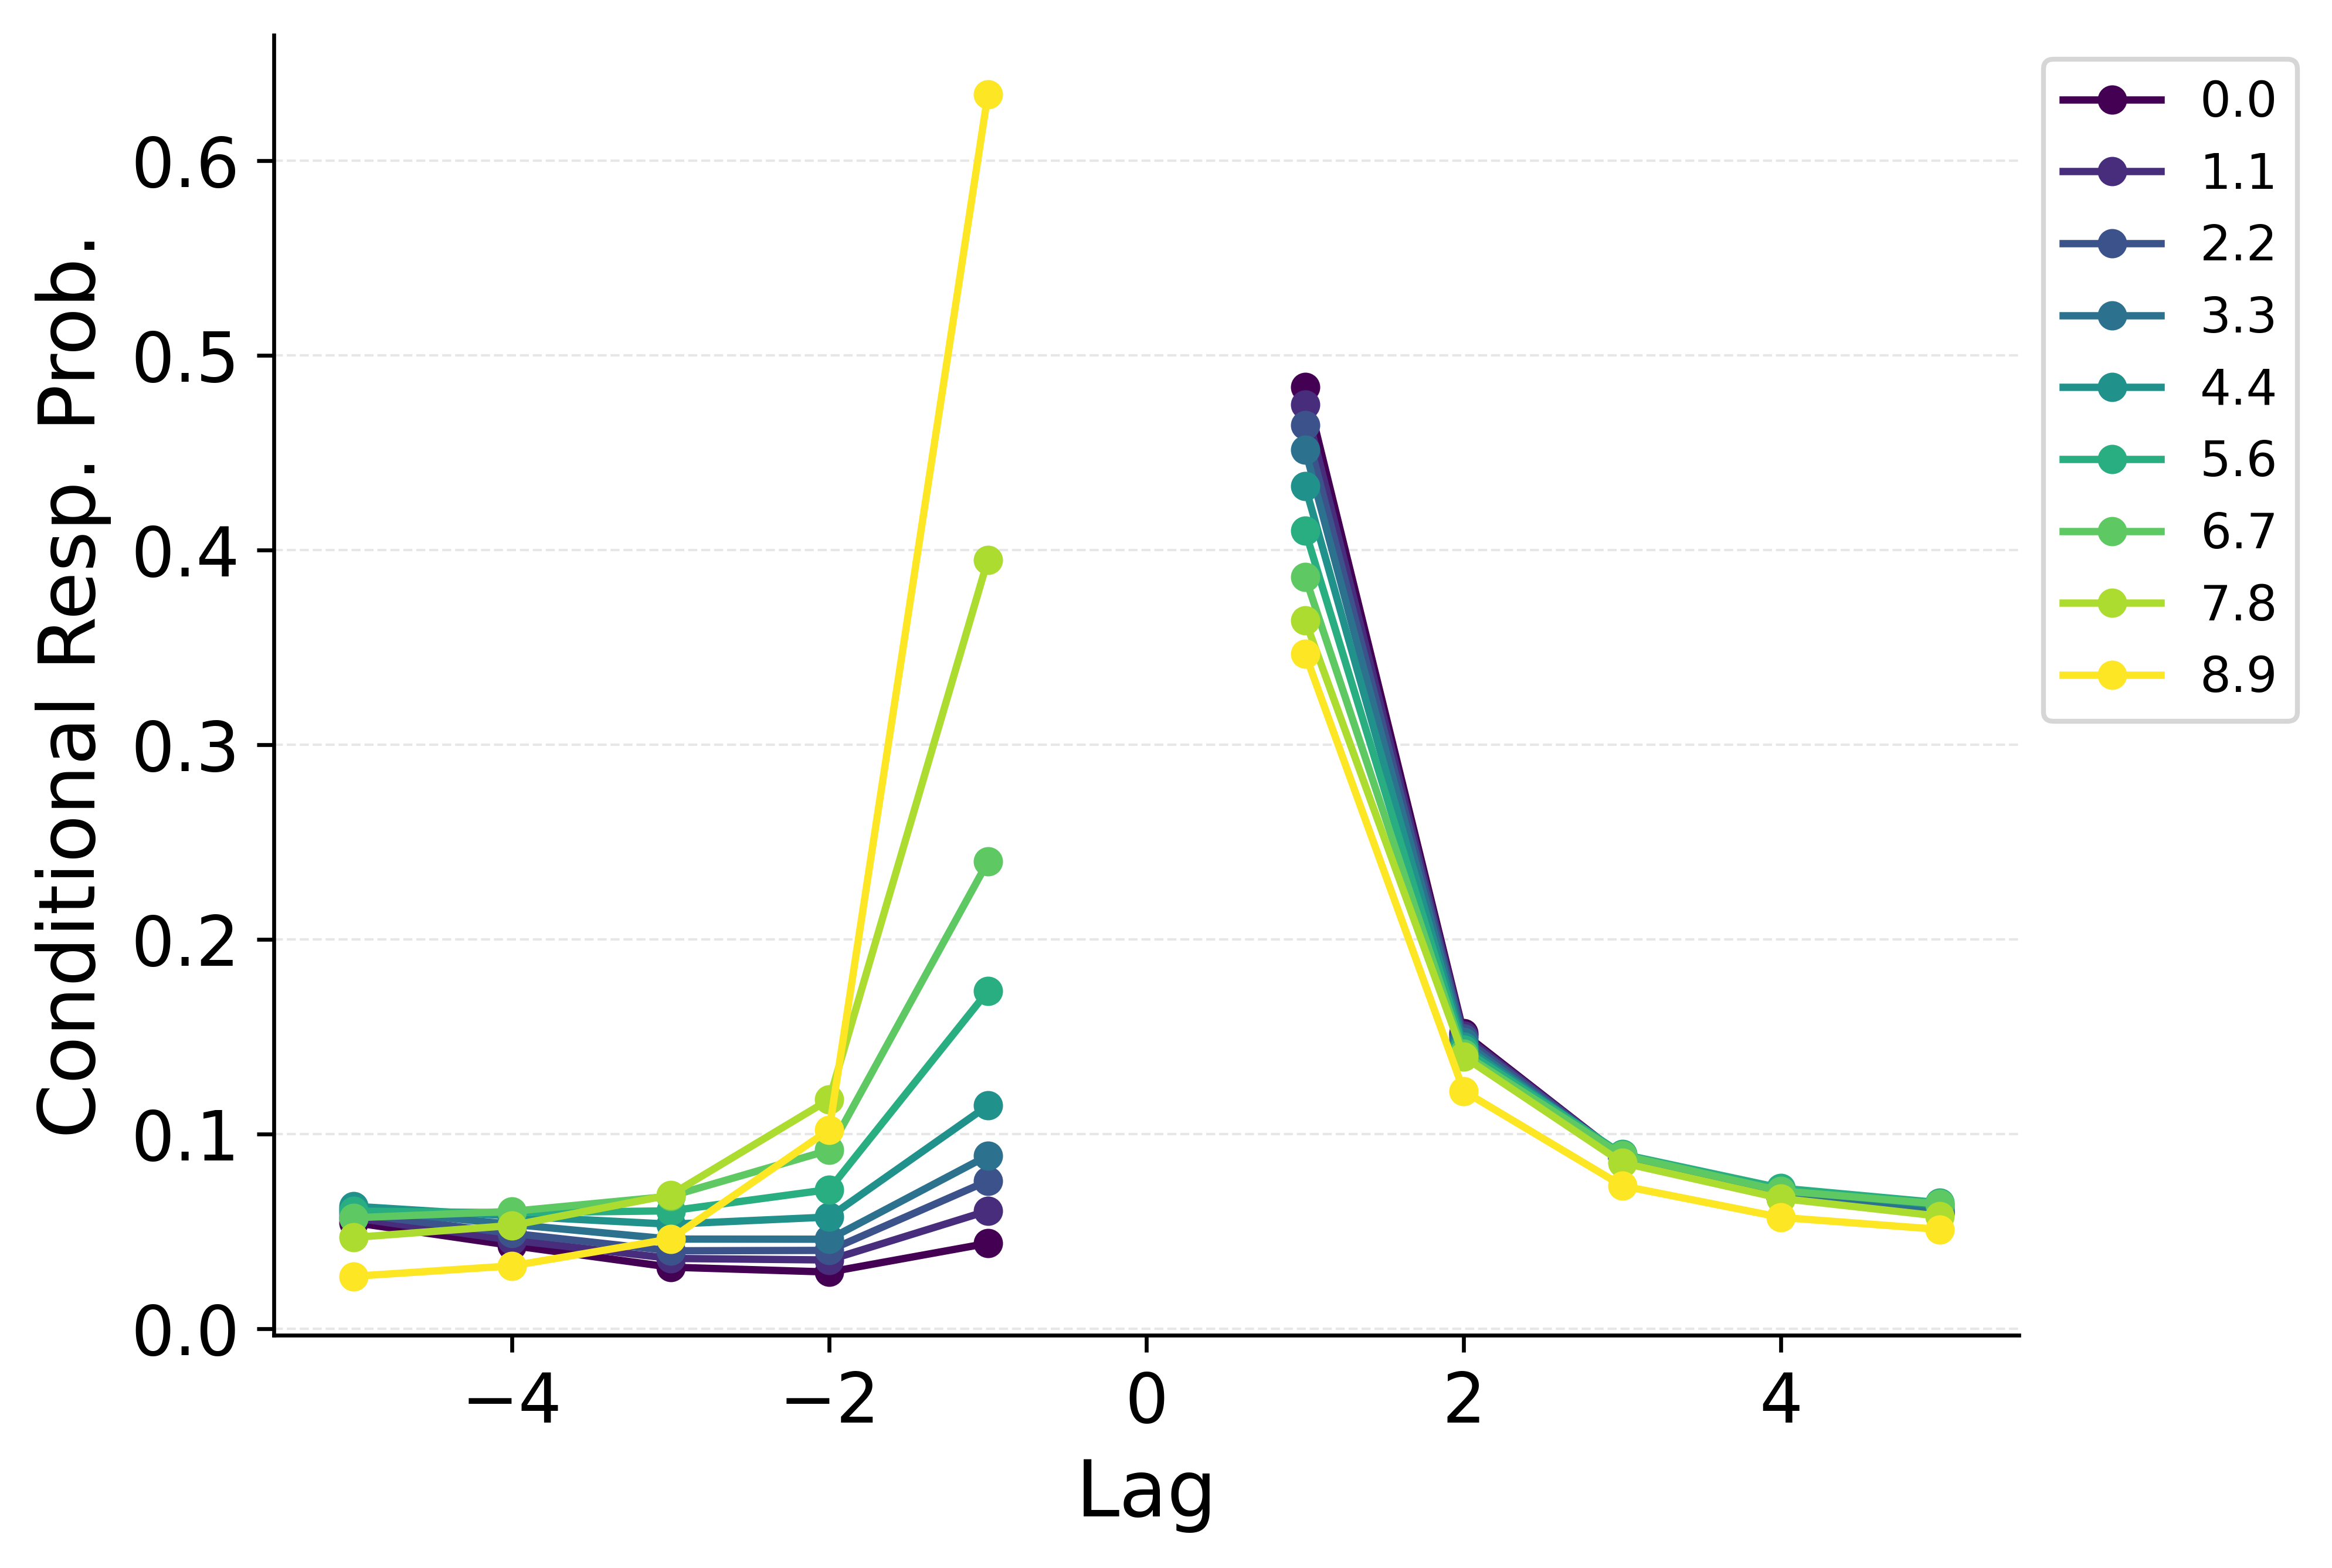
\includegraphics{shifting/BaseCMR_Item_Support_Parameter_Shifting_crp_HealeyKahana2014.png}\end{minipage}%

\end{figure}%

\subsection{Position- vs Context-Based Mechanisms for Recall
Termination}\label{position--vs-context-based-mechanisms-for-recall-termination}

\begin{figure}

\caption{\label{fig-freetermination}Summary statistic fits of CMR with
CRU's context-based recall termination mechanism to Healey and Kahana
(\citeproc{ref-healey2014memory}{2014}). \textbf{Left}: probability of
starting recall by serial position. \textbf{Middle}: conditional
response probability as a function of lag. \textbf{Right}: recall
probability by serial position.}

\begin{minipage}{0.33\linewidth}
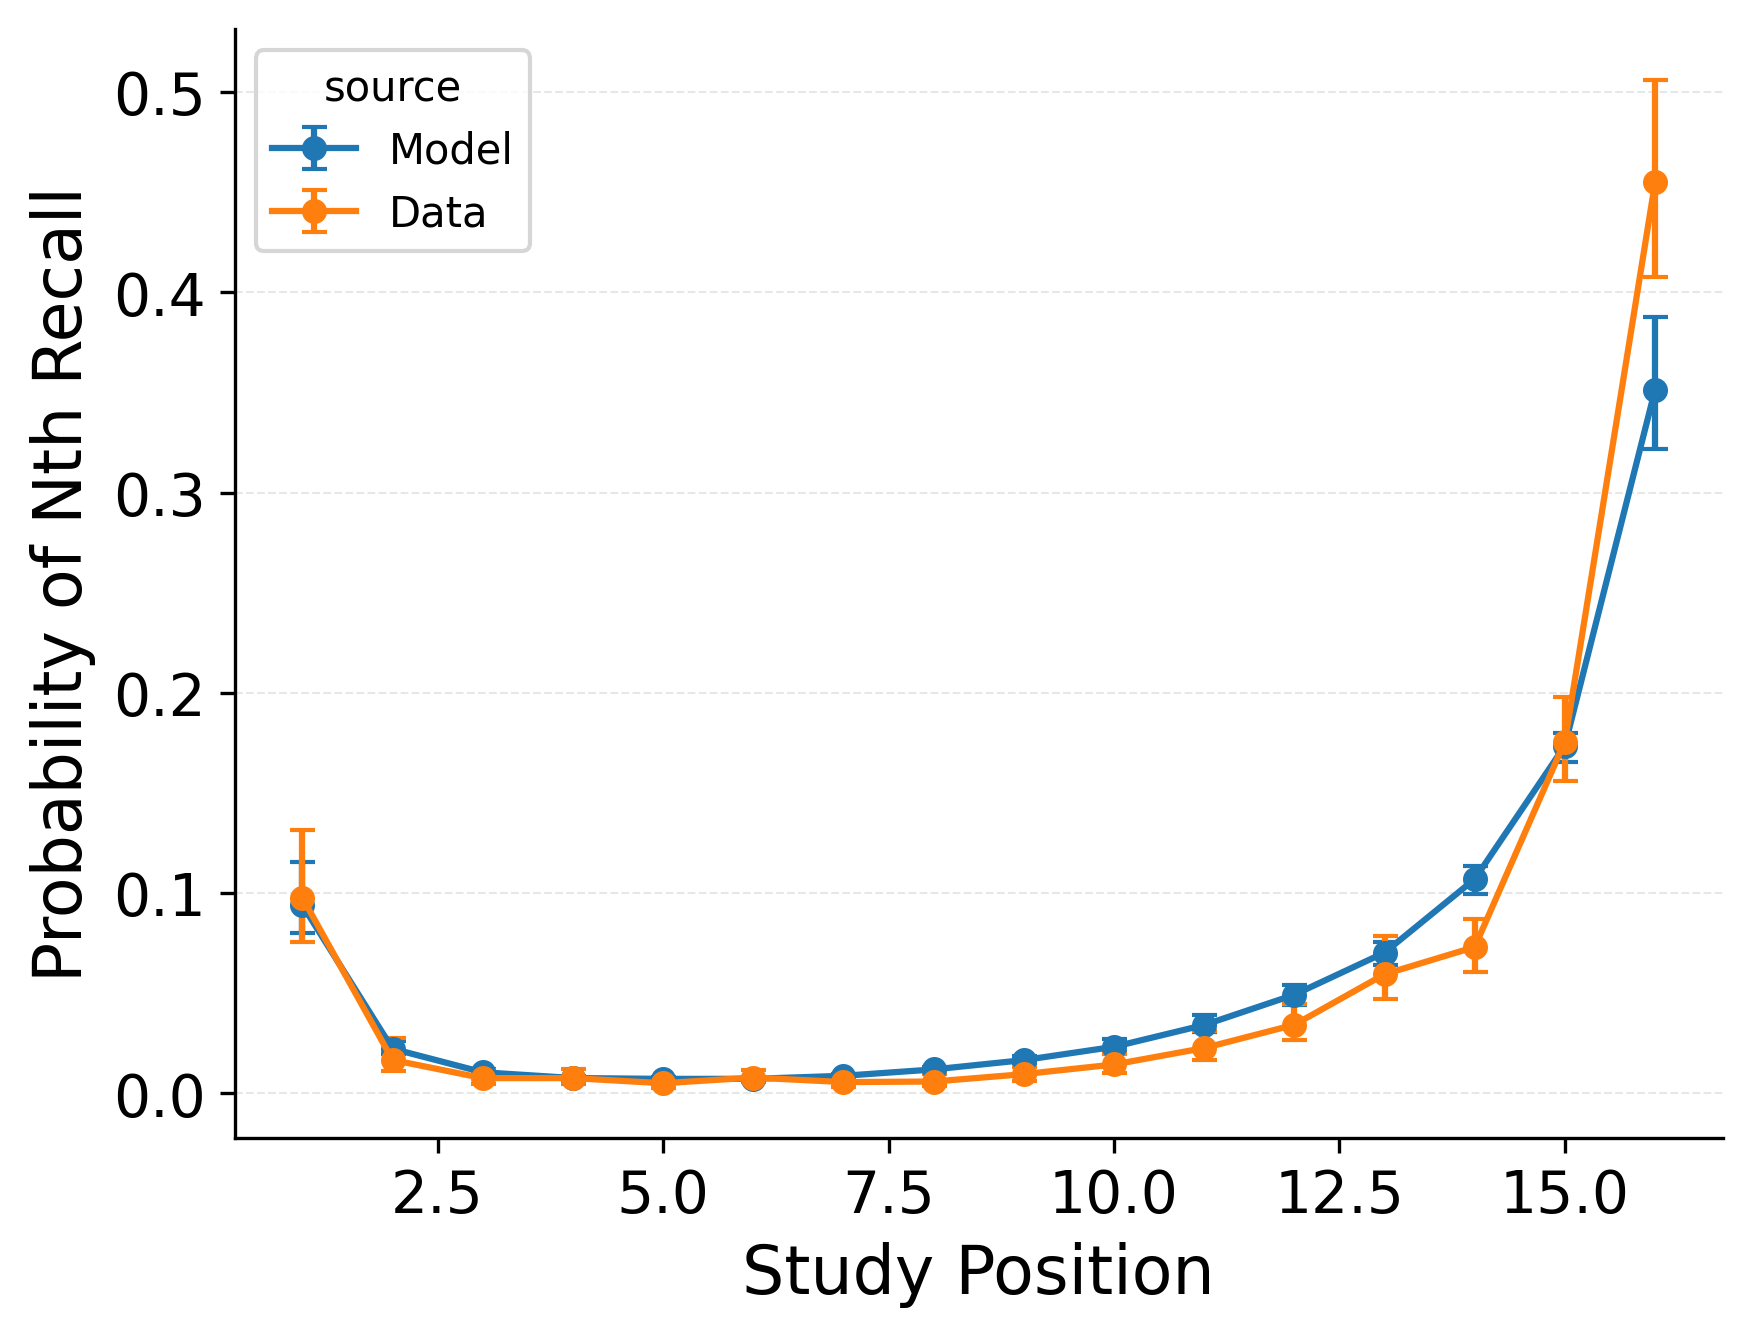
\includegraphics{figures/HealeyKahana2014_CRU_with_Feature-to-Context__Pre-Expt__Primacy_StartDrift__and_ContextTerm_Fitting_pnr.png}\end{minipage}%
%
\begin{minipage}{0.33\linewidth}
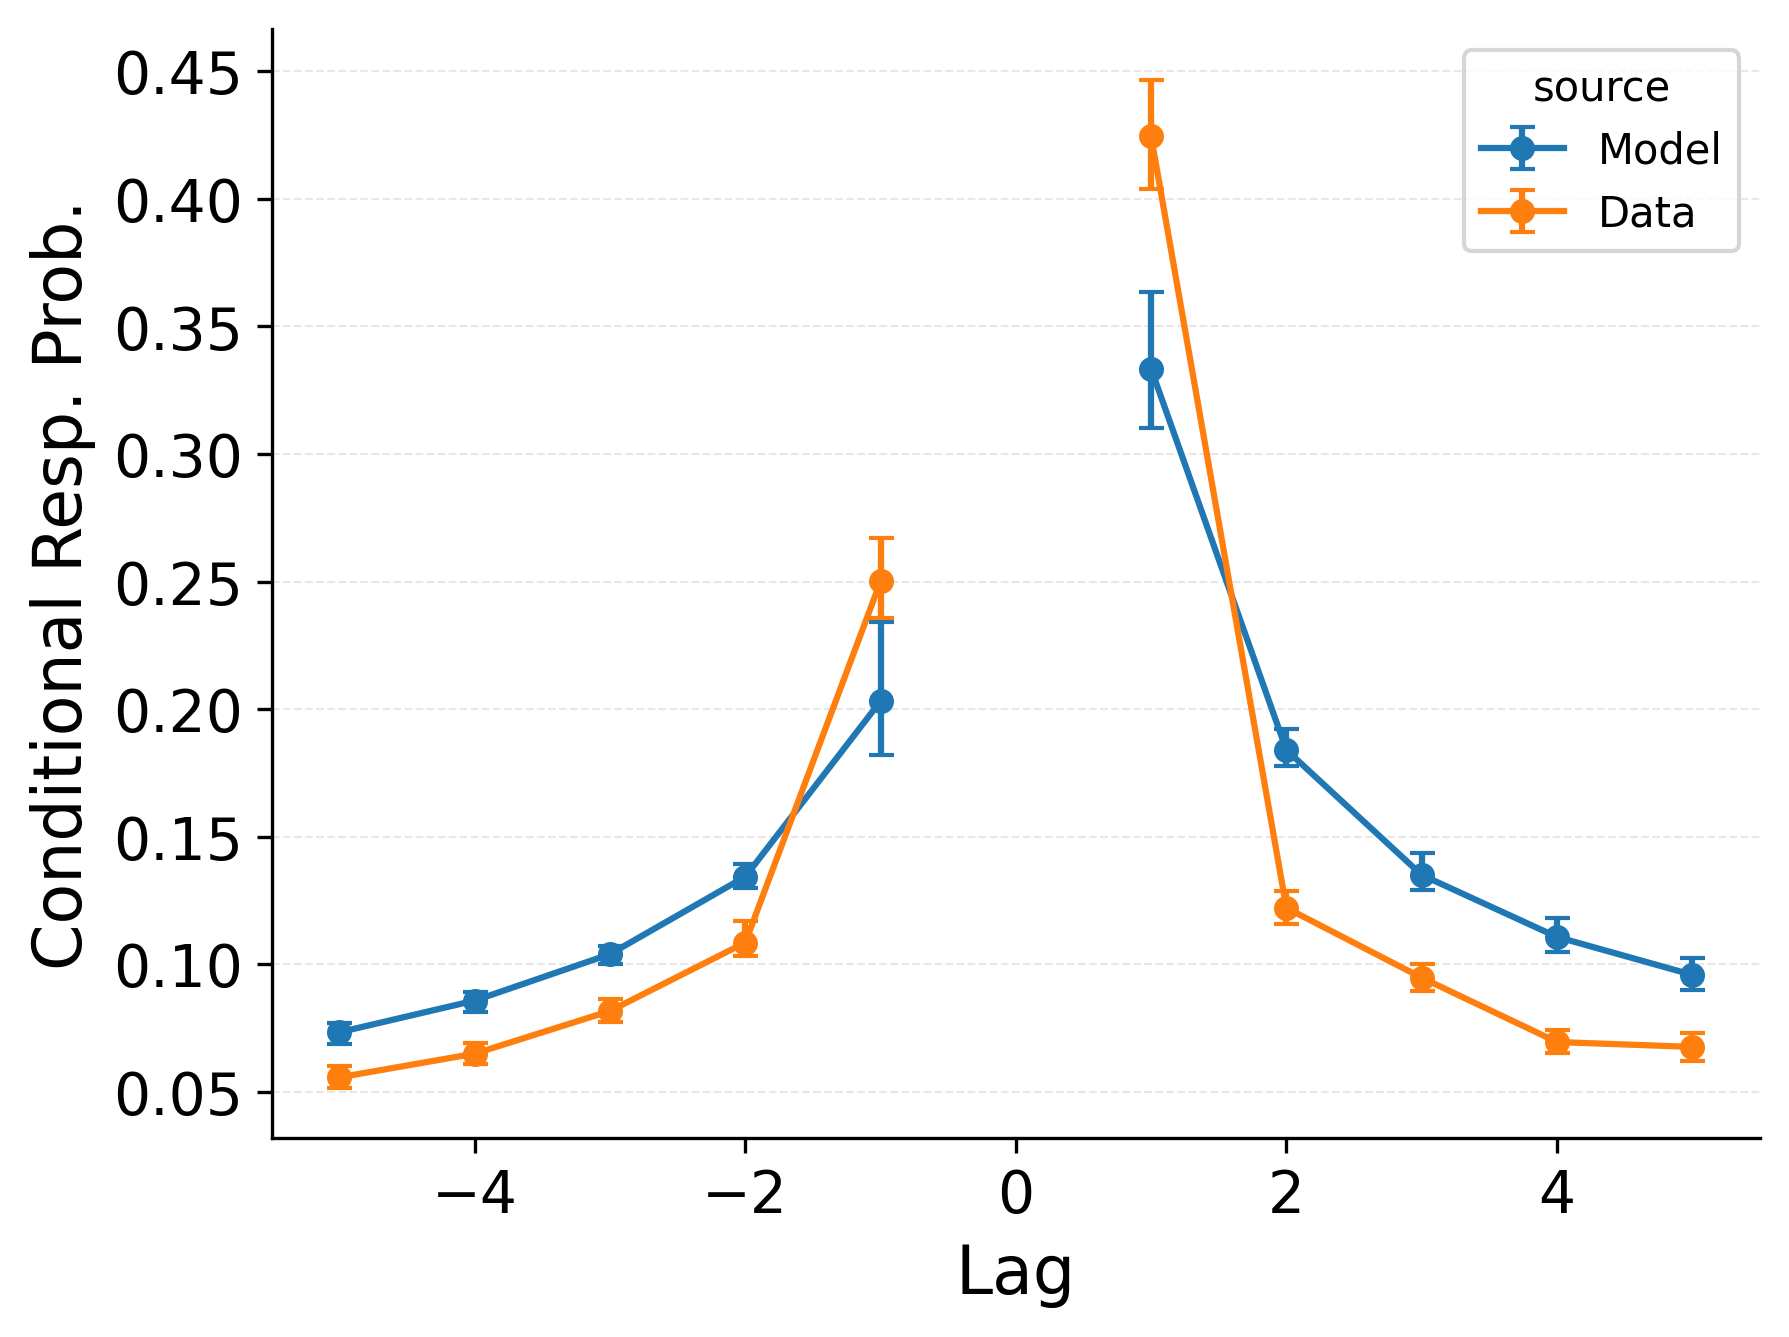
\includegraphics{figures/HealeyKahana2014_CRU_with_Feature-to-Context__Pre-Expt__Primacy_StartDrift__and_ContextTerm_Fitting_crp.png}\end{minipage}%
%
\begin{minipage}{0.33\linewidth}
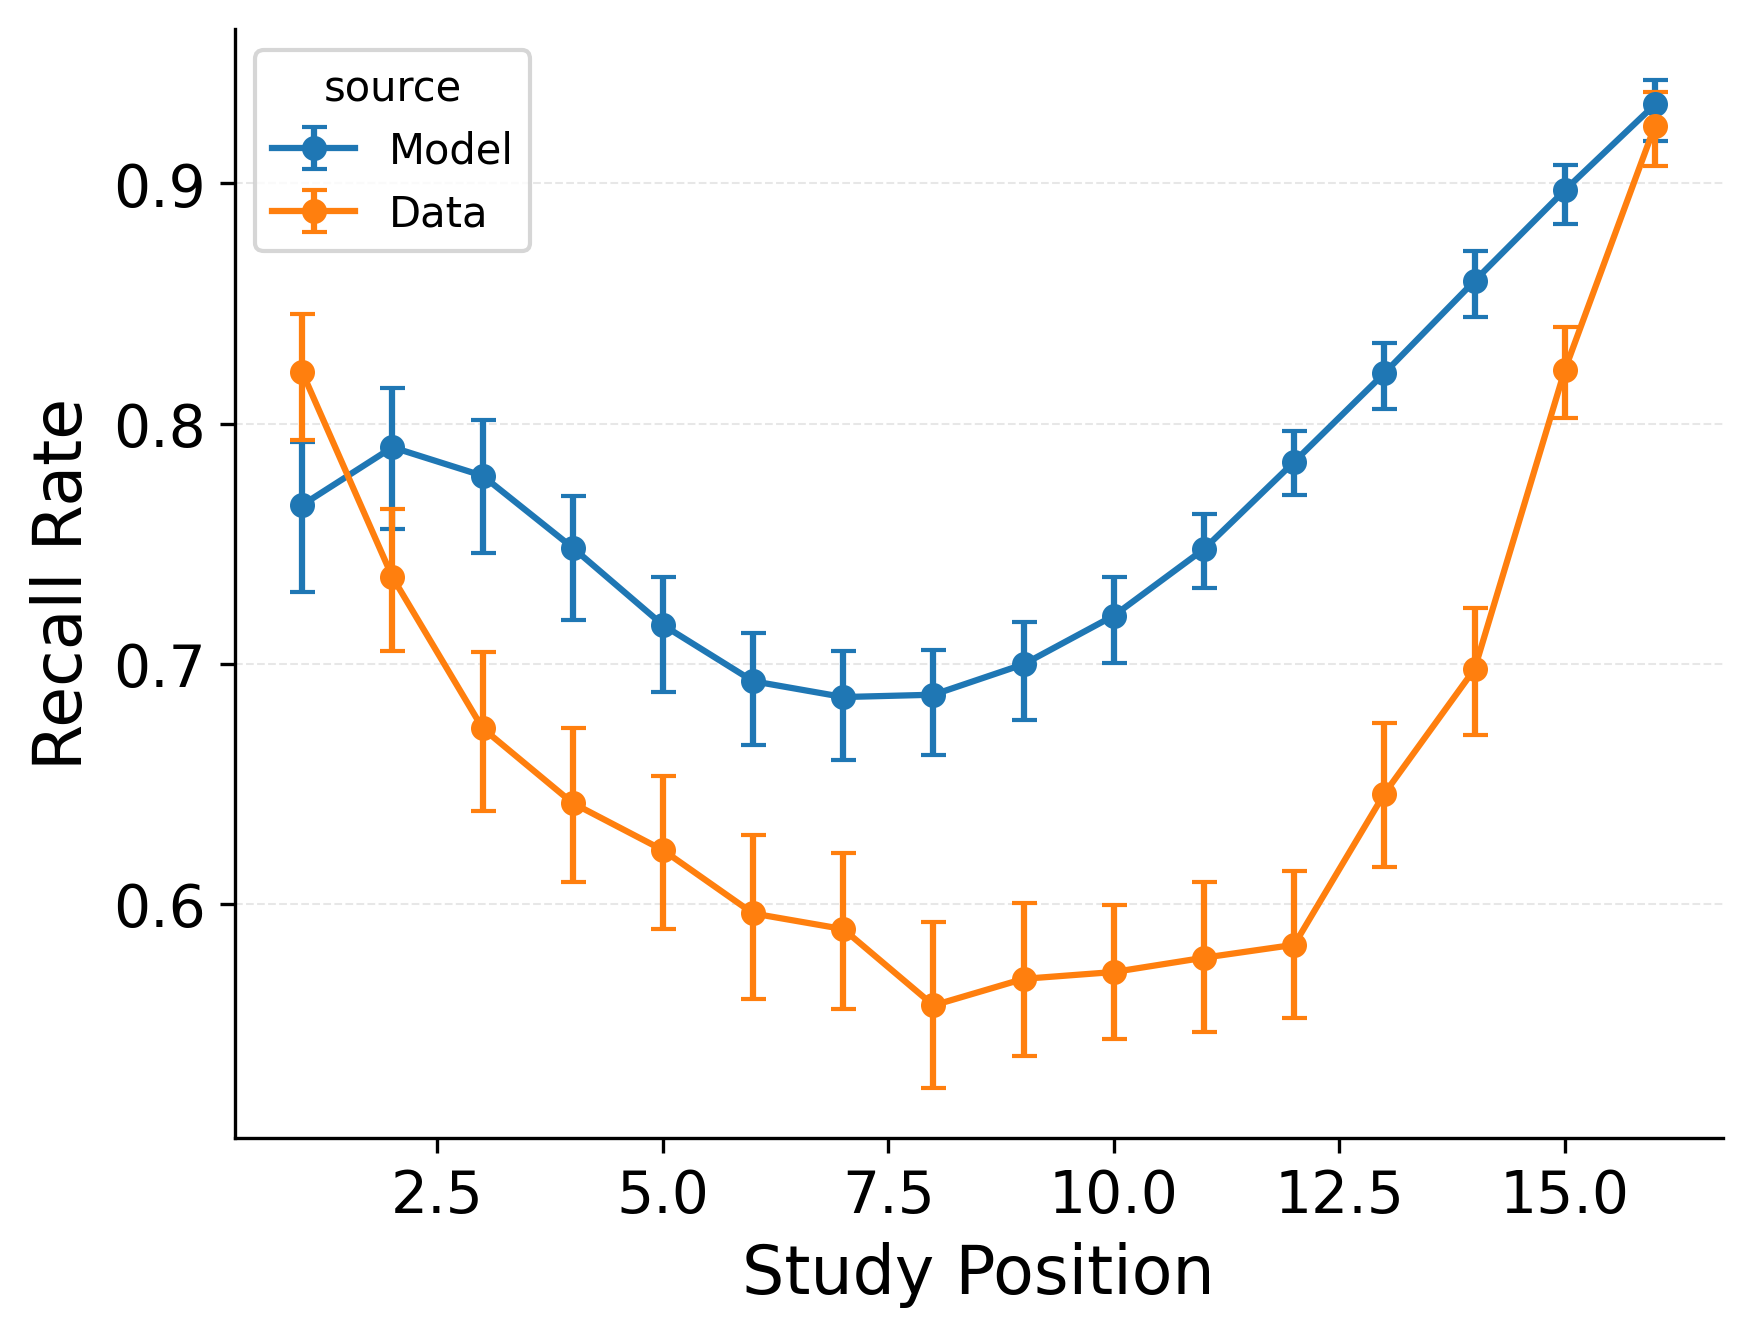
\includegraphics{figures/HealeyKahana2014_CRU_with_Feature-to-Context__Pre-Expt__Primacy_StartDrift__and_ContextTerm_Fitting_spc.png}\end{minipage}%

\end{figure}%

CRU and CMR's mechanisms for recall termination are fundamentally
different. This difference cannot be captured by toggling a parameter
from a fixed to a freely adjustable value, but rather, these mechanisms
can only be swapped between variants. CMR uses exponentially increasing
stopping probabilities \(\theta_\text{s}\) and \(\theta_\text{r}\) to
model recall termination; the probability of termination scales only
with the number of recalls made so far. By contrast, CRU treats the end
of a study sequence as a special item associated in memory with the
final state of the study context. This item competes with other items
for retrieval at each new recall event, and its activation can terminate
recall. In this specification, the probability of termination depends on
the state of context at each recall event, and can be influenced by the
same mechanisms that influence the probability of recalling other items.

Performance differences between CMR's position-based recall termination
mechanism and CRU's context-based recall termination mechanism are
substantial. While Figure~\ref{fig-cmr} shows baseline CMR's performance
on these benchmarks, Figure~\ref{fig-freetermination} shows the
performance of CMR with CRU's context-based recall termination
mechanism. While patterns in response initiation are well-captured,
using context-based recall termination mechanism leads CMR to predict
overly high recall rates for all study list positions and to fail to
capture the sharpness of the lag-contiguity effect. The success of CRU's
context-based recall termination mechanism depends on how consistently
participants terminate recall after recalling the final items from the
study list. In most serial recall datasets, participants tend to perform
this way, and the mechanism correspondingly predicts that the
probability of terminating recall scales with the number of recalls made
so far, as context drifts from its start-of-list state to its
end-of-list state. By contrast, in free recall datasets where
participants exhibit a strong recency effect in recall initiation, this
mechanism can predict early termination of recall upon or even before
retrieving the last item in the study list.

\section{Serial Recall Results}\label{serial-recall-results}

\begin{table}

{\caption{{Negative log-likelihood (±95\% CI) averaged across
participants for selected model variants fit to the Logan
(\citeproc{ref-logan2021serial}{2021}) dataset. \(\gamma\):
item-to-context learning rate; \(\alpha\): shared support; \(\delta\):
self-support; \(\phi_\text{s}\): primacy scale; \(\phi_\text{d}\):
primacy decay; \(\beta_\text{start}\): start context integration rate.
All CRU variants in this table use the context-based end-of-list
termination mechanism unless otherwise noted.}{\label{tbl-fits-serial}}}
\vspace{-20pt}}

\begin{longtable}[]{@{}
  >{\raggedright\arraybackslash}p{(\columnwidth - 2\tabcolsep) * \real{0.7083}}
  >{\raggedright\arraybackslash}p{(\columnwidth - 2\tabcolsep) * \real{0.2917}}@{}}
\toprule\noalign{}
\begin{minipage}[b]{\linewidth}\raggedright
Model Variant
\end{minipage} & \begin{minipage}[b]{\linewidth}\raggedright
−LL (±95\% CI)
\end{minipage} \\
\midrule\noalign{}
\endhead
\bottomrule\noalign{}
\endlastfoot
CRU with Free \(\alpha\), \(\delta\), \(\phi_\text{s}\),
\(\phi_\text{d}\) & 1428.98 ± 222.09 \\
CMR with CRU's Context-Based Termination & 1431.39 ± 223.74 \\
CRU with Free \(\gamma\), \(\alpha\), \(\delta\) & 1436.94 ± 222.11 \\
CRU with Free \(\phi_\text{s}\), \(\phi_\text{d}\),
\(\beta_{\text{start}}\) & 1443.14 ± 221.79 \\
CRU & 1482.94 ± 230.86 \\
CMR with Own Position-Based Termination Rule & 1508.45 ± 208.88 \\
\end{longtable}

\end{table}

Our goal is to determine whether any of the mechanisms that give CMR an
advantage in free recall can improve the fit of CRU to this serial
recall dataset (Expt. 1 from Logan
(\citeproc{ref-logan2021serial}{2021}), described above). Importantly,
we allow item identification confusability via CRU's \(g\) and
\(g_\text{dec}\) parameters to be freely estimated in all model variants
so that intrusion errors can be predicted. Without this mechanism the
likelihood of intrusions is 0. Given the presence of intrusions in the
data, this collapses the fitting process.

The overall goodness of fit for each model variant is presented in
Table~\ref{tbl-fits-serial}. The models are ordered by overall goodness
of fit. These log-likelihood differences are highly reliable at the
group level, based on wAIC comparisons (not reported). The baseline
version of CRU is near the bottom of the list, demonstrating the utility
of adding some mechanisms from CMR to improve model fits. Standard CMR
is at the bottom of the list, demonstrating that some of CRU's
mechanisms are critical to fitting serial recall data. When CRU's recall
termination rule is incorporated into CMR, this improves the model's
performance, but it still falls far short of the best CRU model. The
most successful model is a version of CRU that uses a few CMR
mechanisms: adjustable context-to-feature shared support (\(\alpha\))
and self-support (\(\delta\)) associations, and the associative primacy
gradient (\(\phi_\text{s}\), and \(\phi_\text{d}\)). This model provides
the best fit at the group level as well as for 100\% of the individual
participants in comparison to baseline CRU and CMR with both CRU's
context-based recall termination mechanism and item identification
confusability mechanism. Allowing this version of the model to
additionally adjust the start-of-list context integration
(\(\beta_\text{start}\)) parameter, to adjust the feature-to-context
learning (\(\gamma\)) parameter, or to adjust both parameters, did not
improve model fits. The importance of the associative primacy gradient
parameters for a good fit is demonstrated by the worse fit of the
version of CRU that was not allowed to adjust those parameters.
Similarly, the importance of the alpha and delta parameters is
demonstrated by the worse fit of the version of CRU that could not
adjust those parameters. In the following sections we examine the
ability of a subset of these models to capture different benchmark
serial recall phenomena, which gives insight into how these model
mechanisms give rise to serial recall performance.

\subsection{Serial Recall Accuracy and Error
Rates}\label{serial-recall-accuracy-and-error-rates}

\begin{figure}

\caption{\label{fig-serial-srac}Serial recall accuracy (SRAC) fits to
Logan (\citeproc{ref-logan2021serial}{2021}) serial recall data for list
lengths of 5 (\textbf{Left Column}), 6 (\textbf{Middle Column}), 7
(\textbf{Right Column}) of baseline CRU (\textbf{Top}), the best
performing CRU variant with free pre-experimental context-to-feature
memory (\(\alpha\), \(\delta\)) and CMR-specific primacy gradient
(\(\phi_\text{s}\), \(\phi_\text{d}\)) parameters (\textbf{Middle}), and
CMR with its default position-based recall termination mechanism and
CRU's item identification confusability mechanism (\textbf{Bottom}).}

\begin{minipage}{0.33\linewidth}
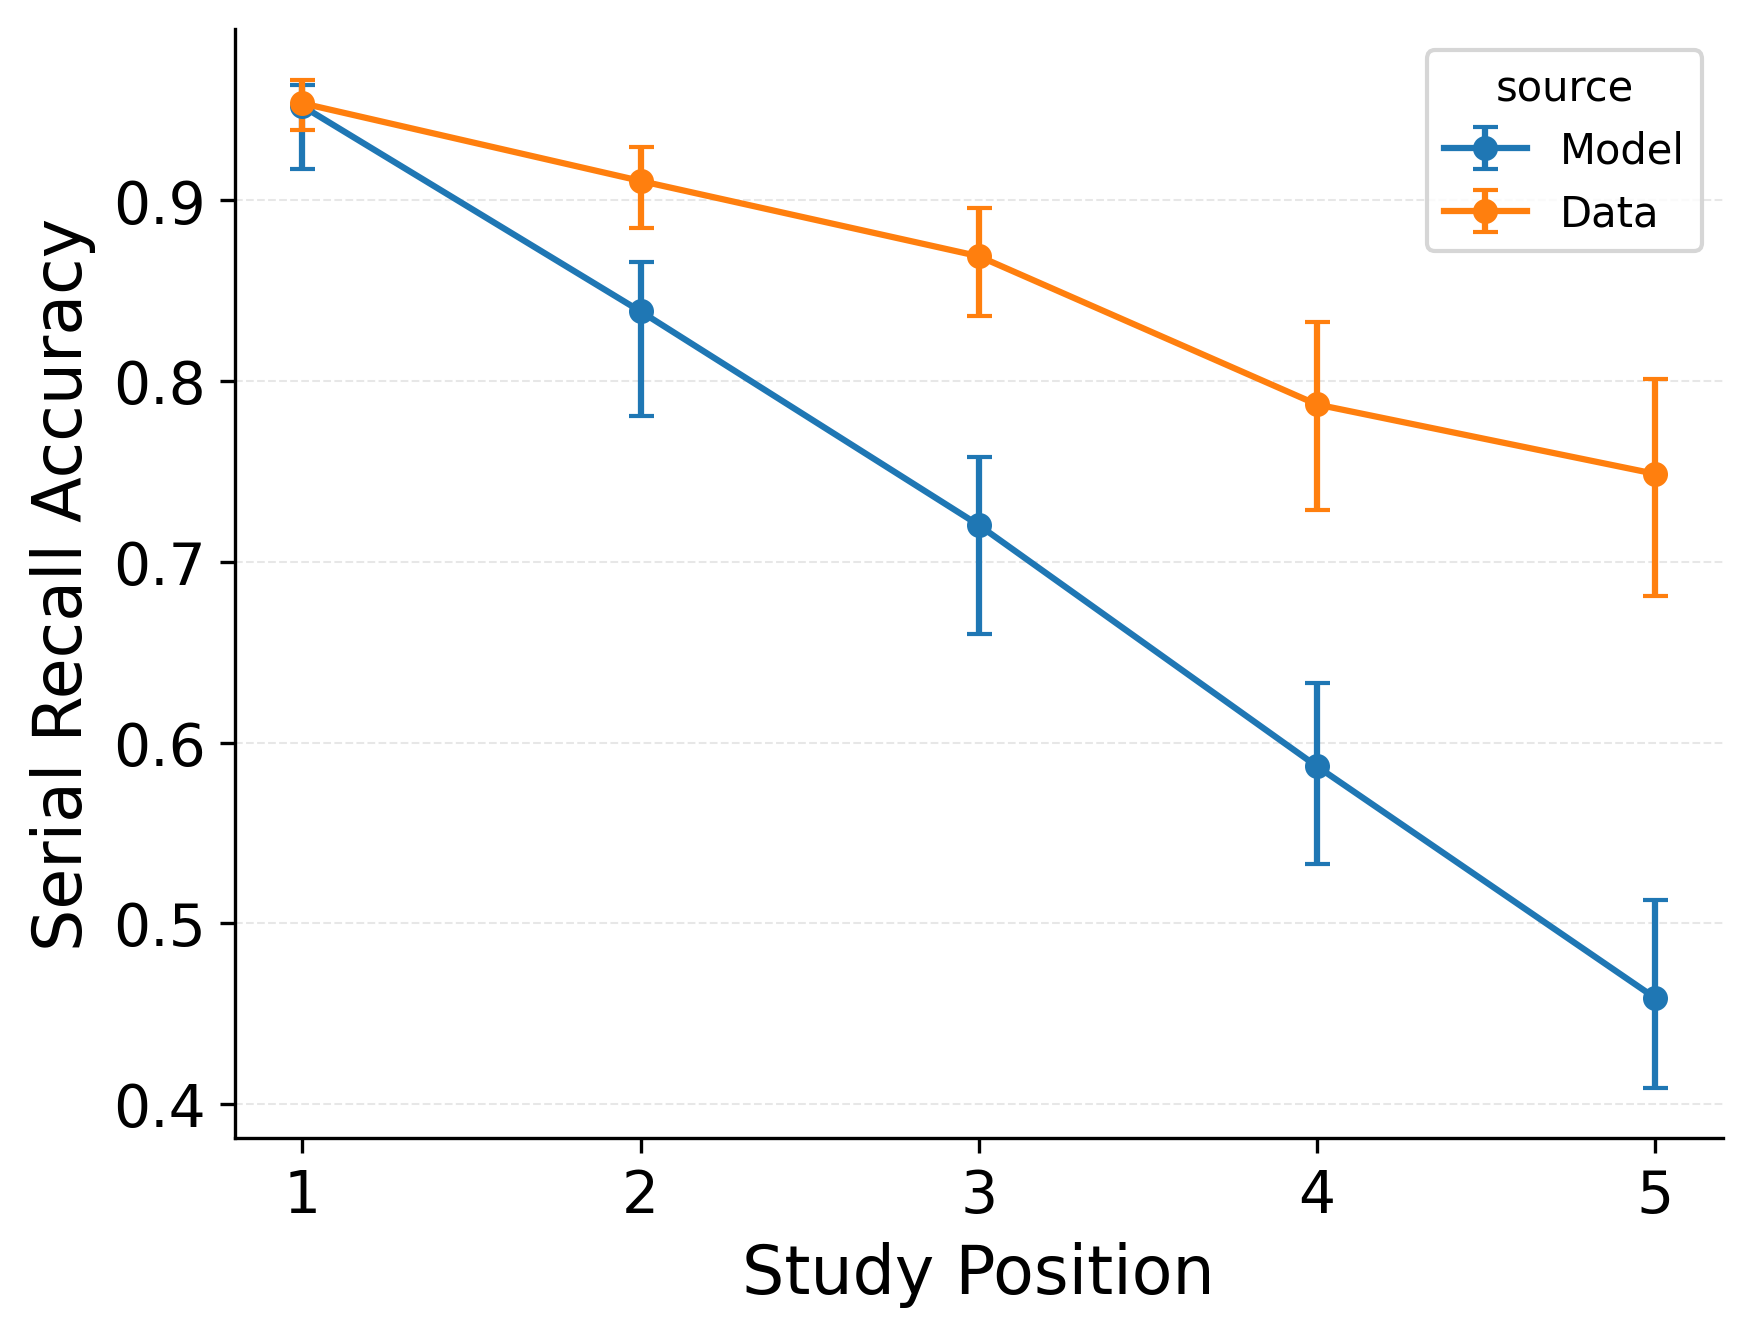
\includegraphics{figures/Gordon2021_BaseCRU_with_ContextTerm_Confusable_Fitting_srac_LL5.png}\end{minipage}%
%
\begin{minipage}{0.33\linewidth}
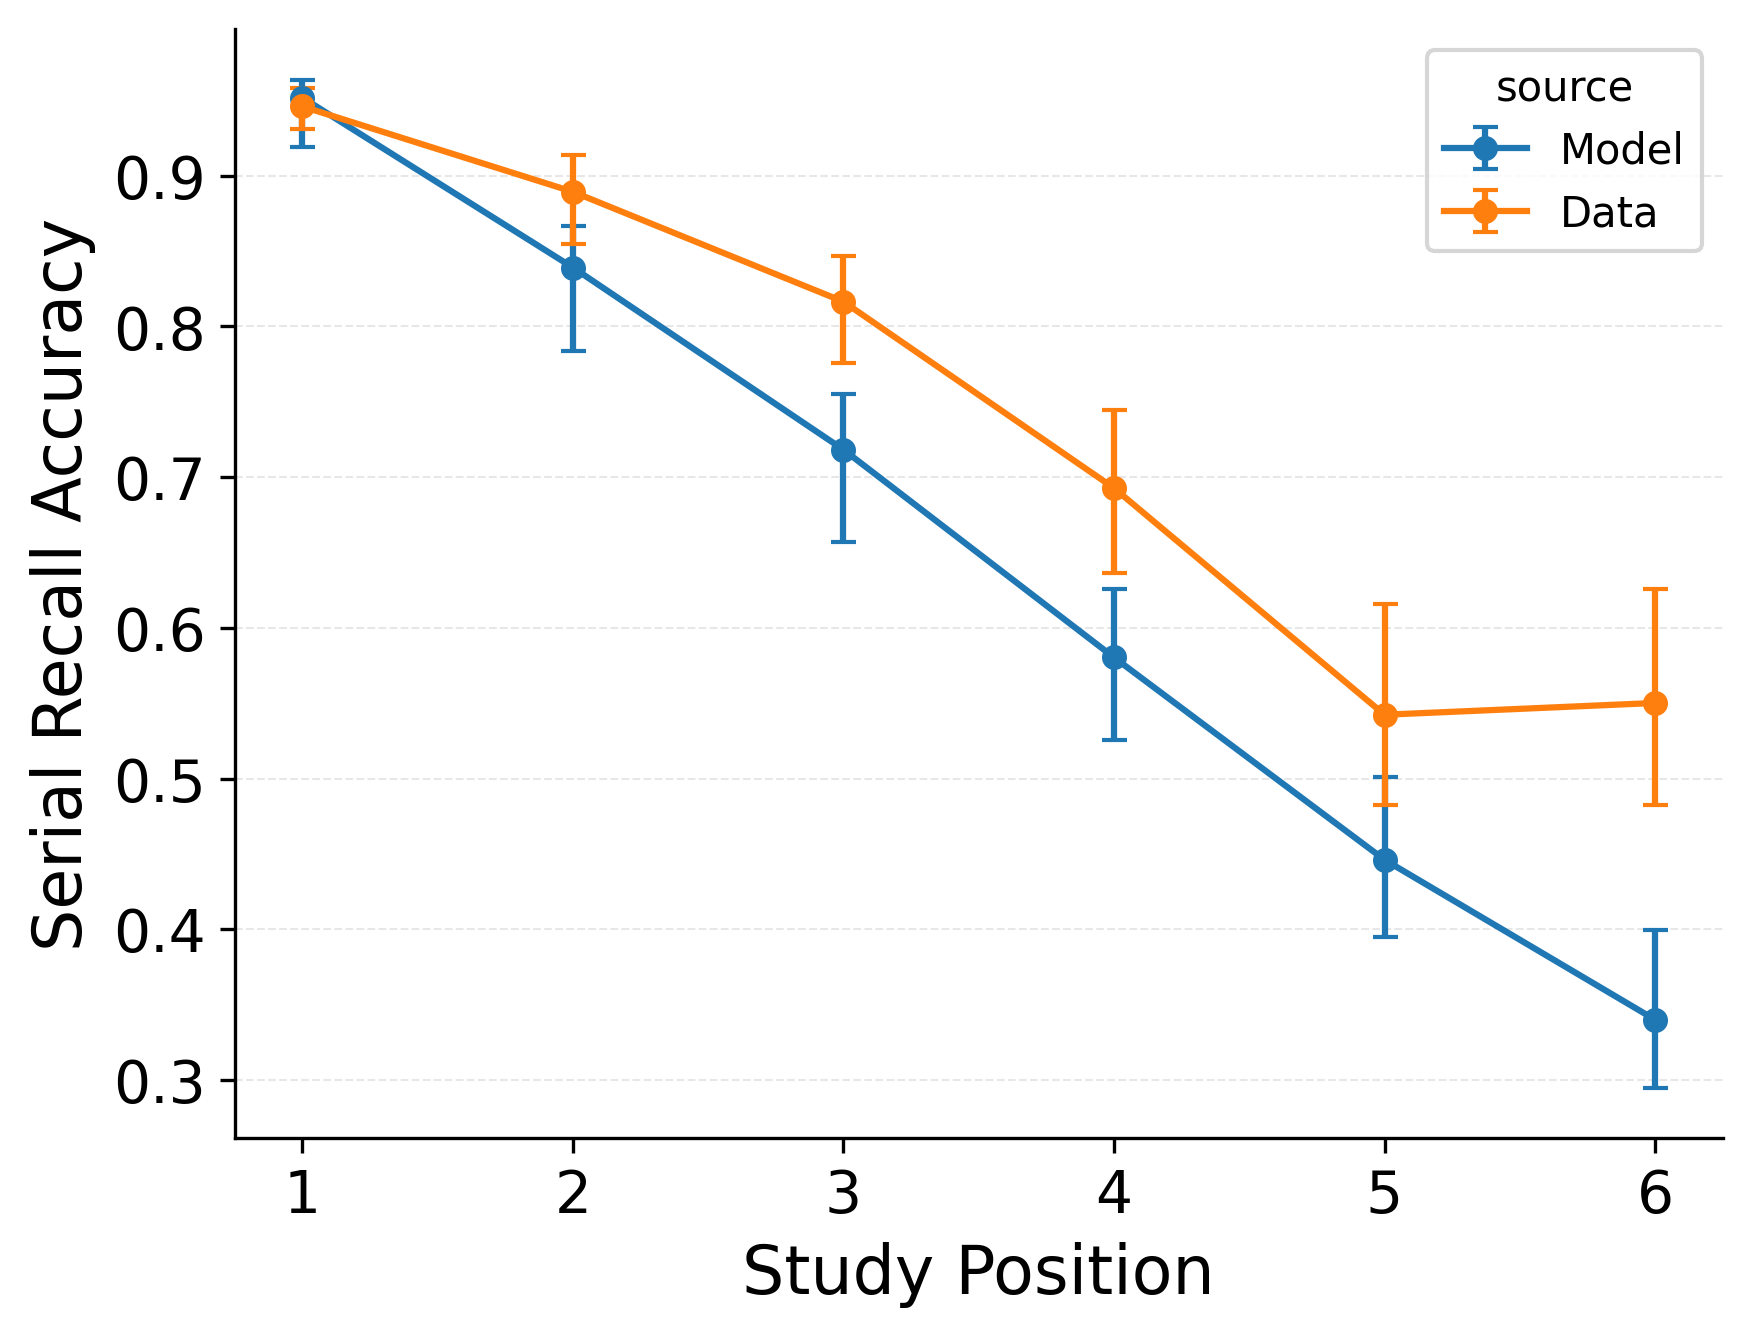
\includegraphics{figures/Gordon2021_BaseCRU_with_ContextTerm_Confusable_Fitting_srac_LL6.png}\end{minipage}%
%
\begin{minipage}{0.33\linewidth}
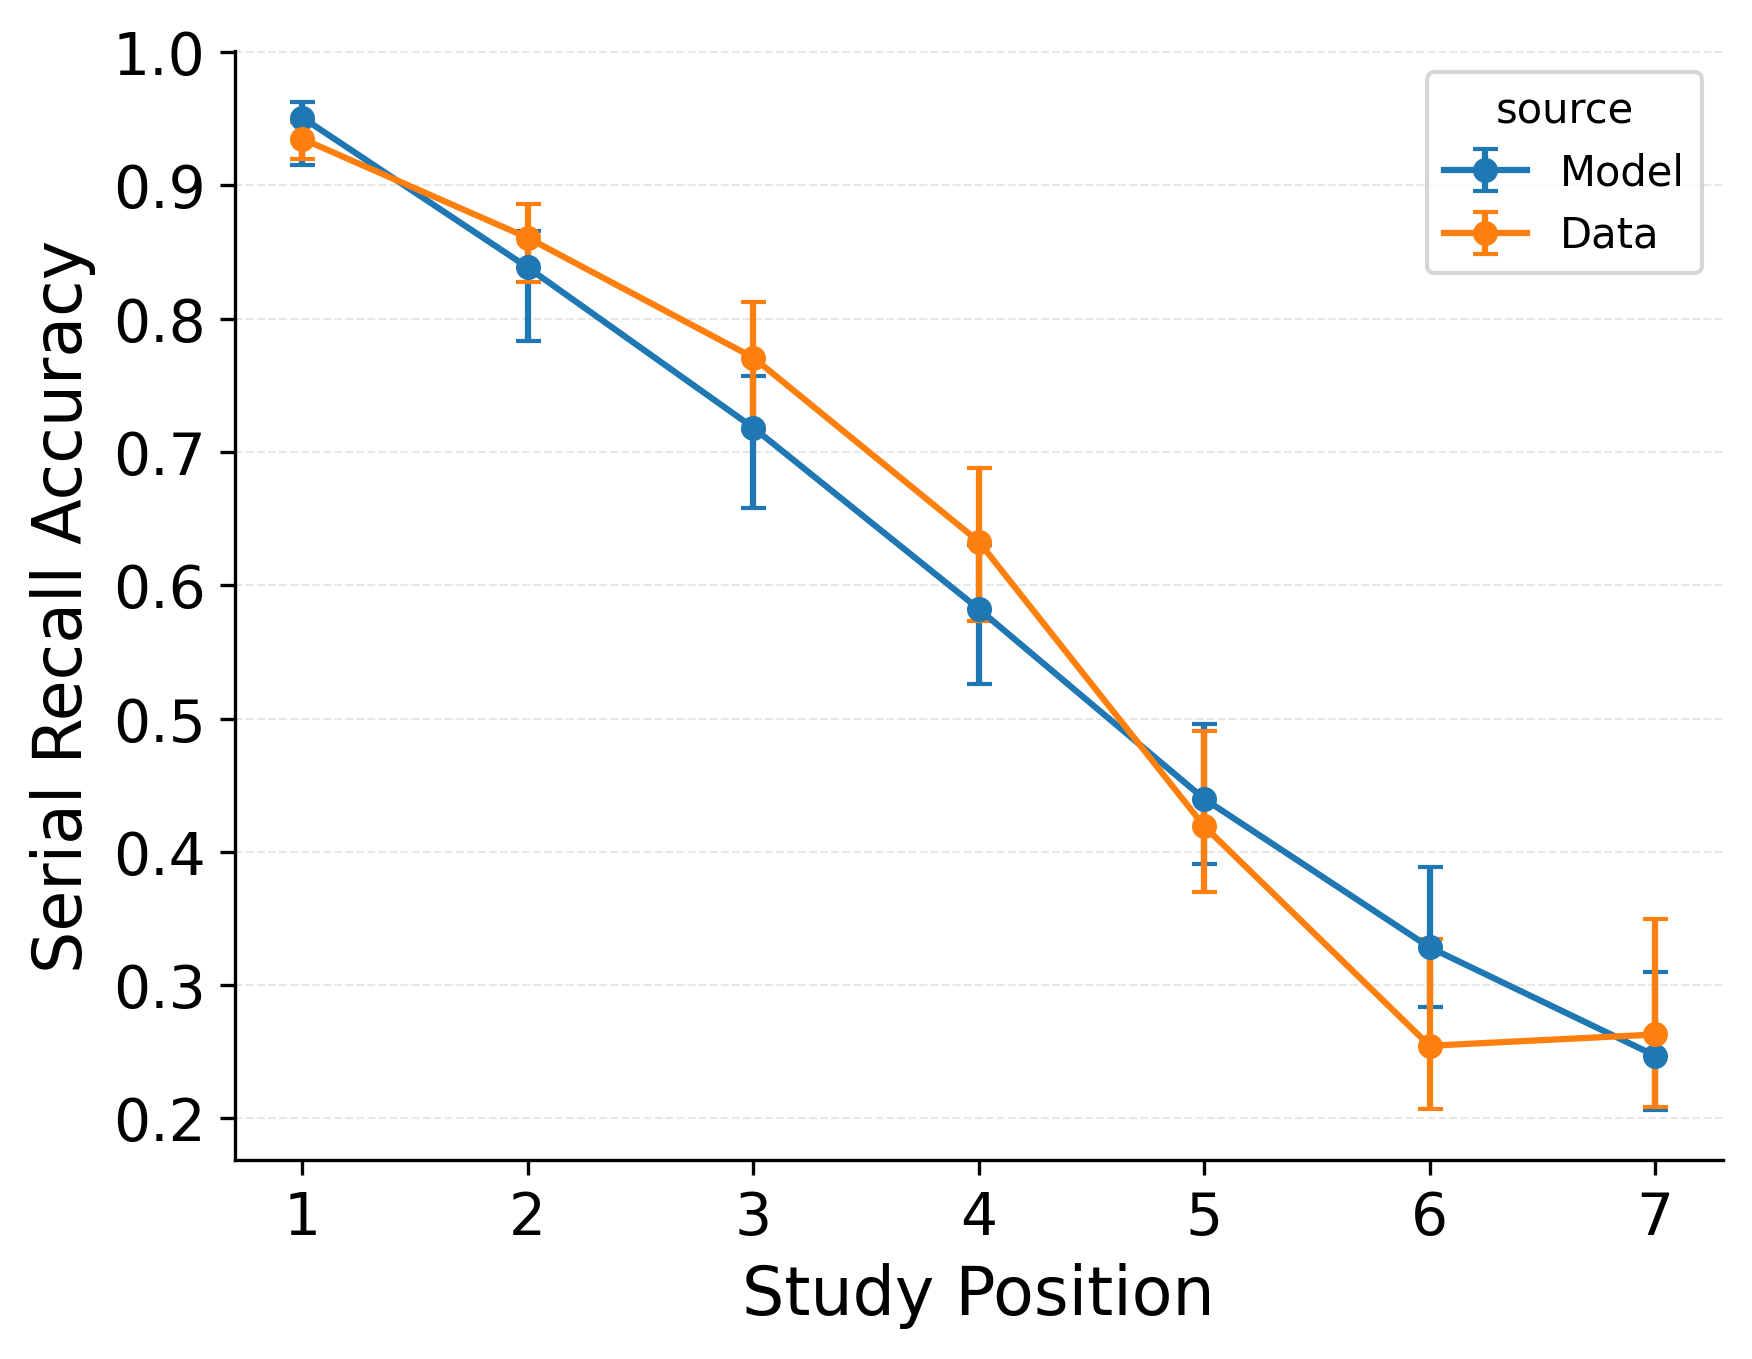
\includegraphics{figures/Gordon2021_BaseCRU_with_ContextTerm_Confusable_Fitting_srac_LL7.png}\end{minipage}%
\newline
\begin{minipage}{0.33\linewidth}
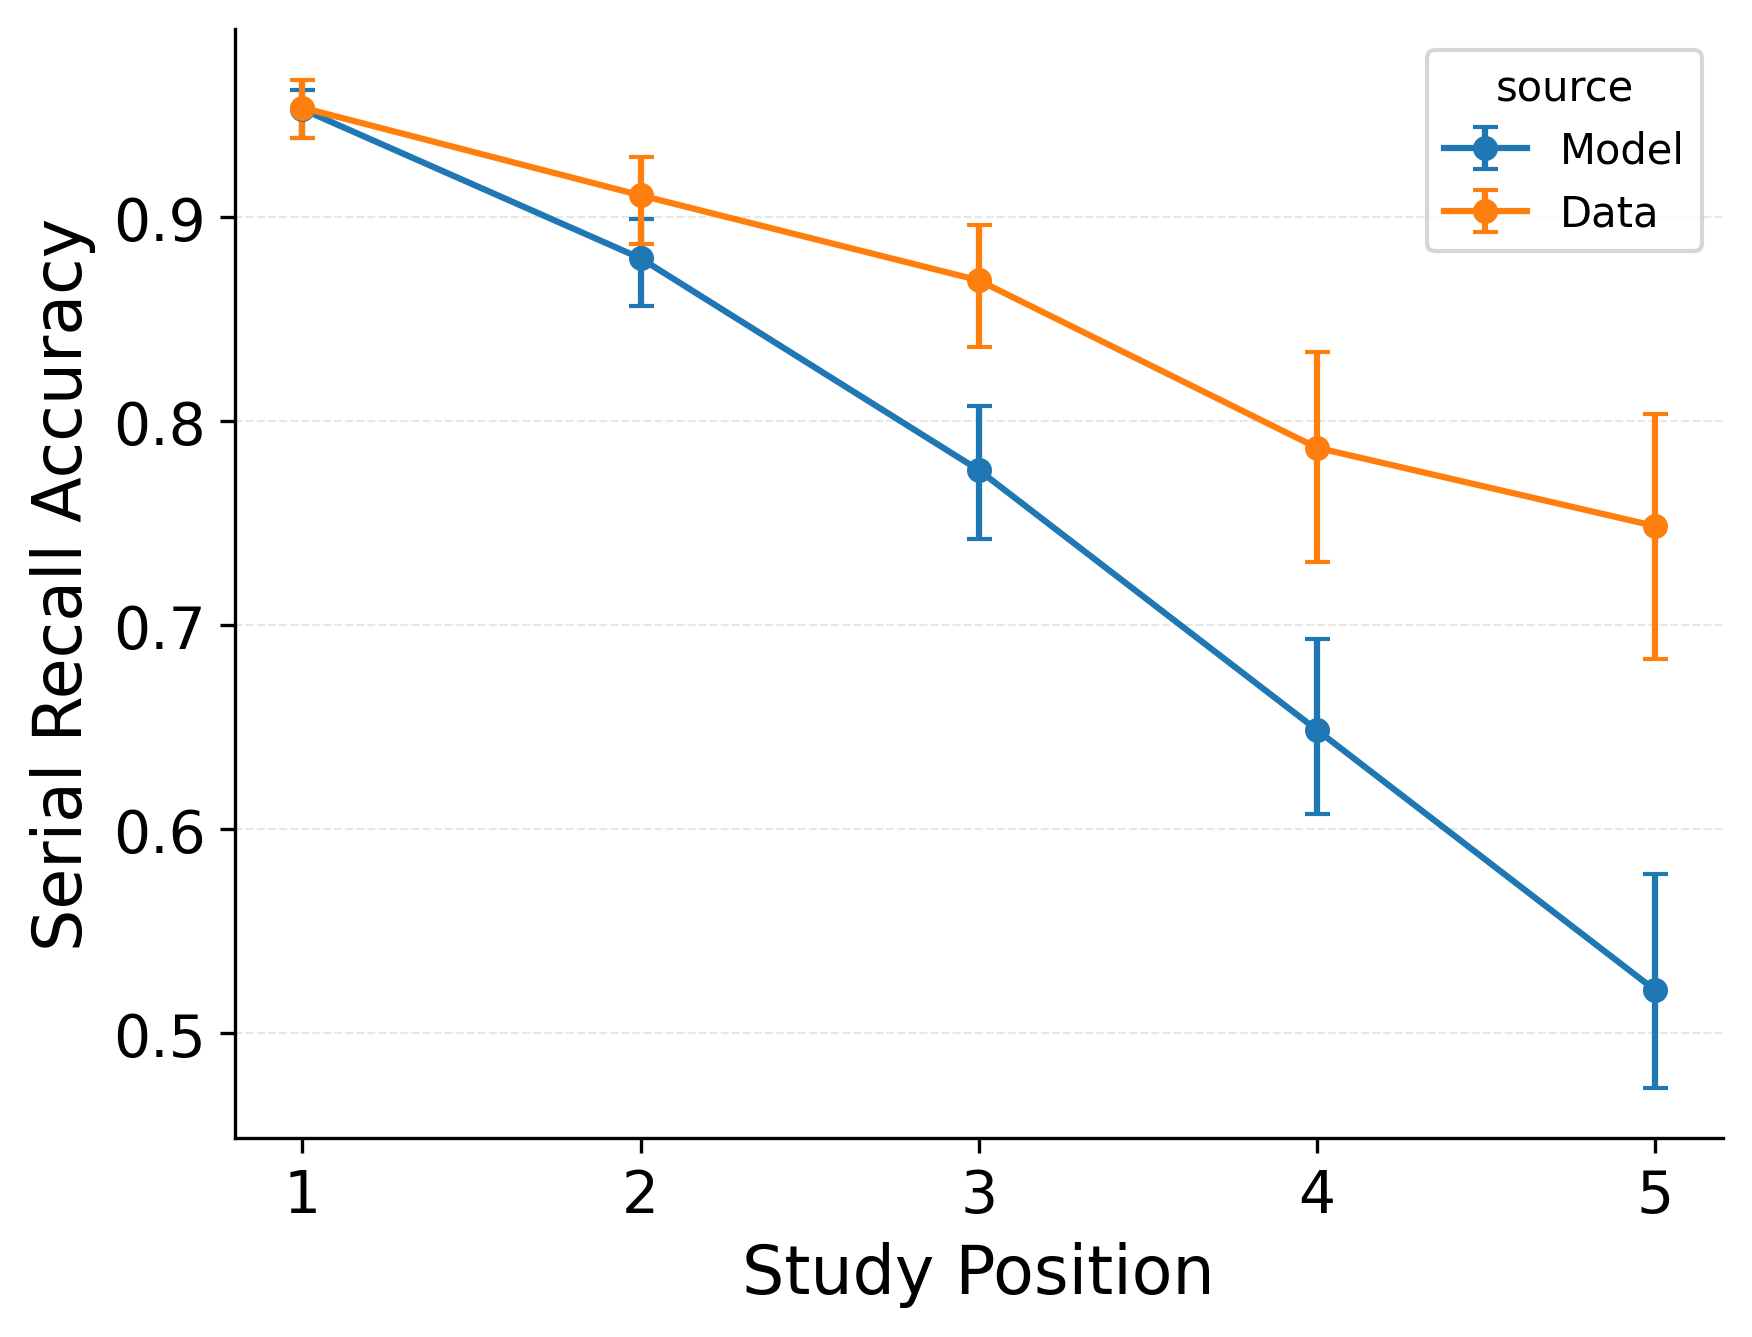
\includegraphics{figures/Gordon2021_CRU_with_Pre-Expt_and_Primacy__and_ContextTerm_Confusable_Fitting_srac_LL5.png}\end{minipage}%
%
\begin{minipage}{0.33\linewidth}
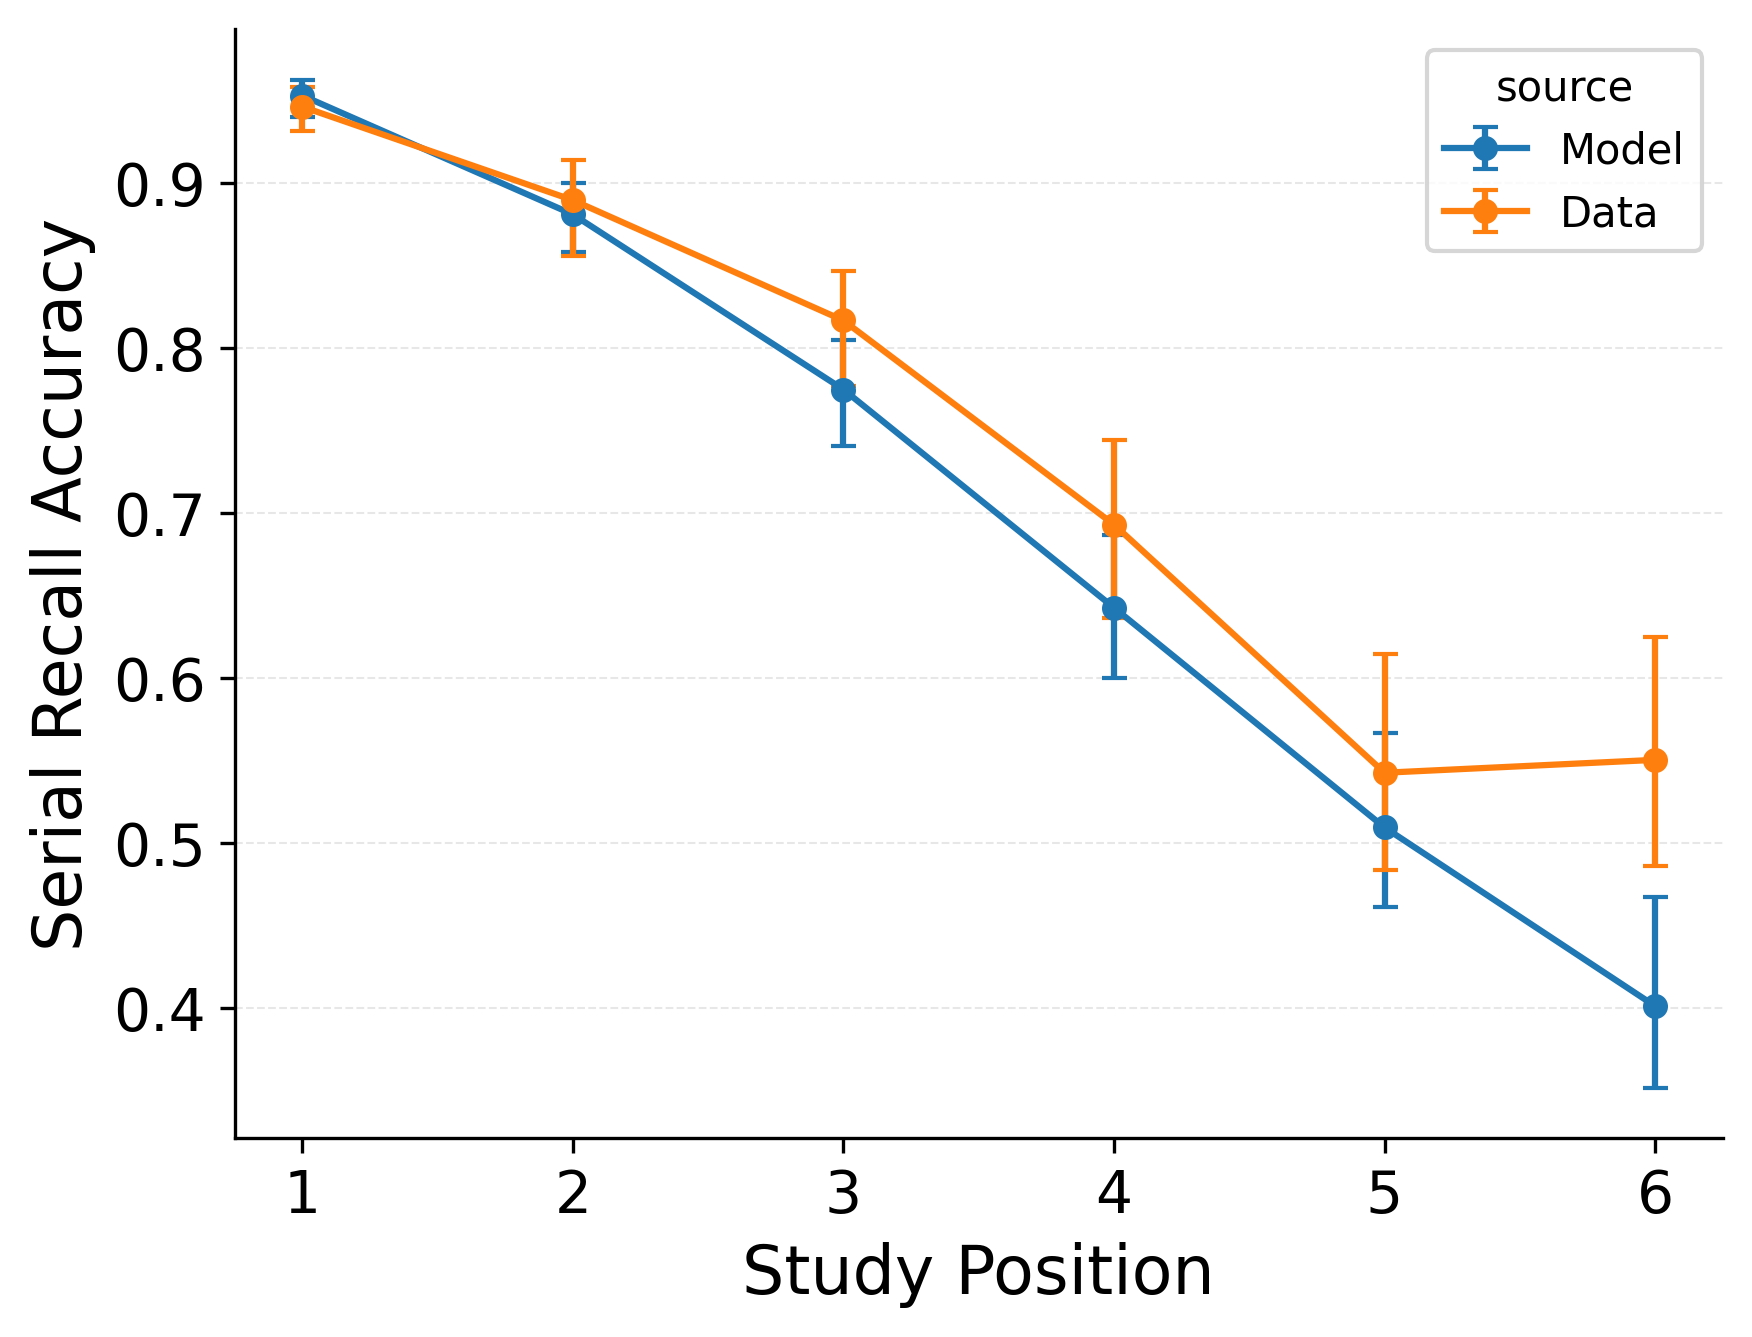
\includegraphics{figures/Gordon2021_CRU_with_Pre-Expt_and_Primacy__and_ContextTerm_Confusable_Fitting_srac_LL6.png}\end{minipage}%
%
\begin{minipage}{0.33\linewidth}
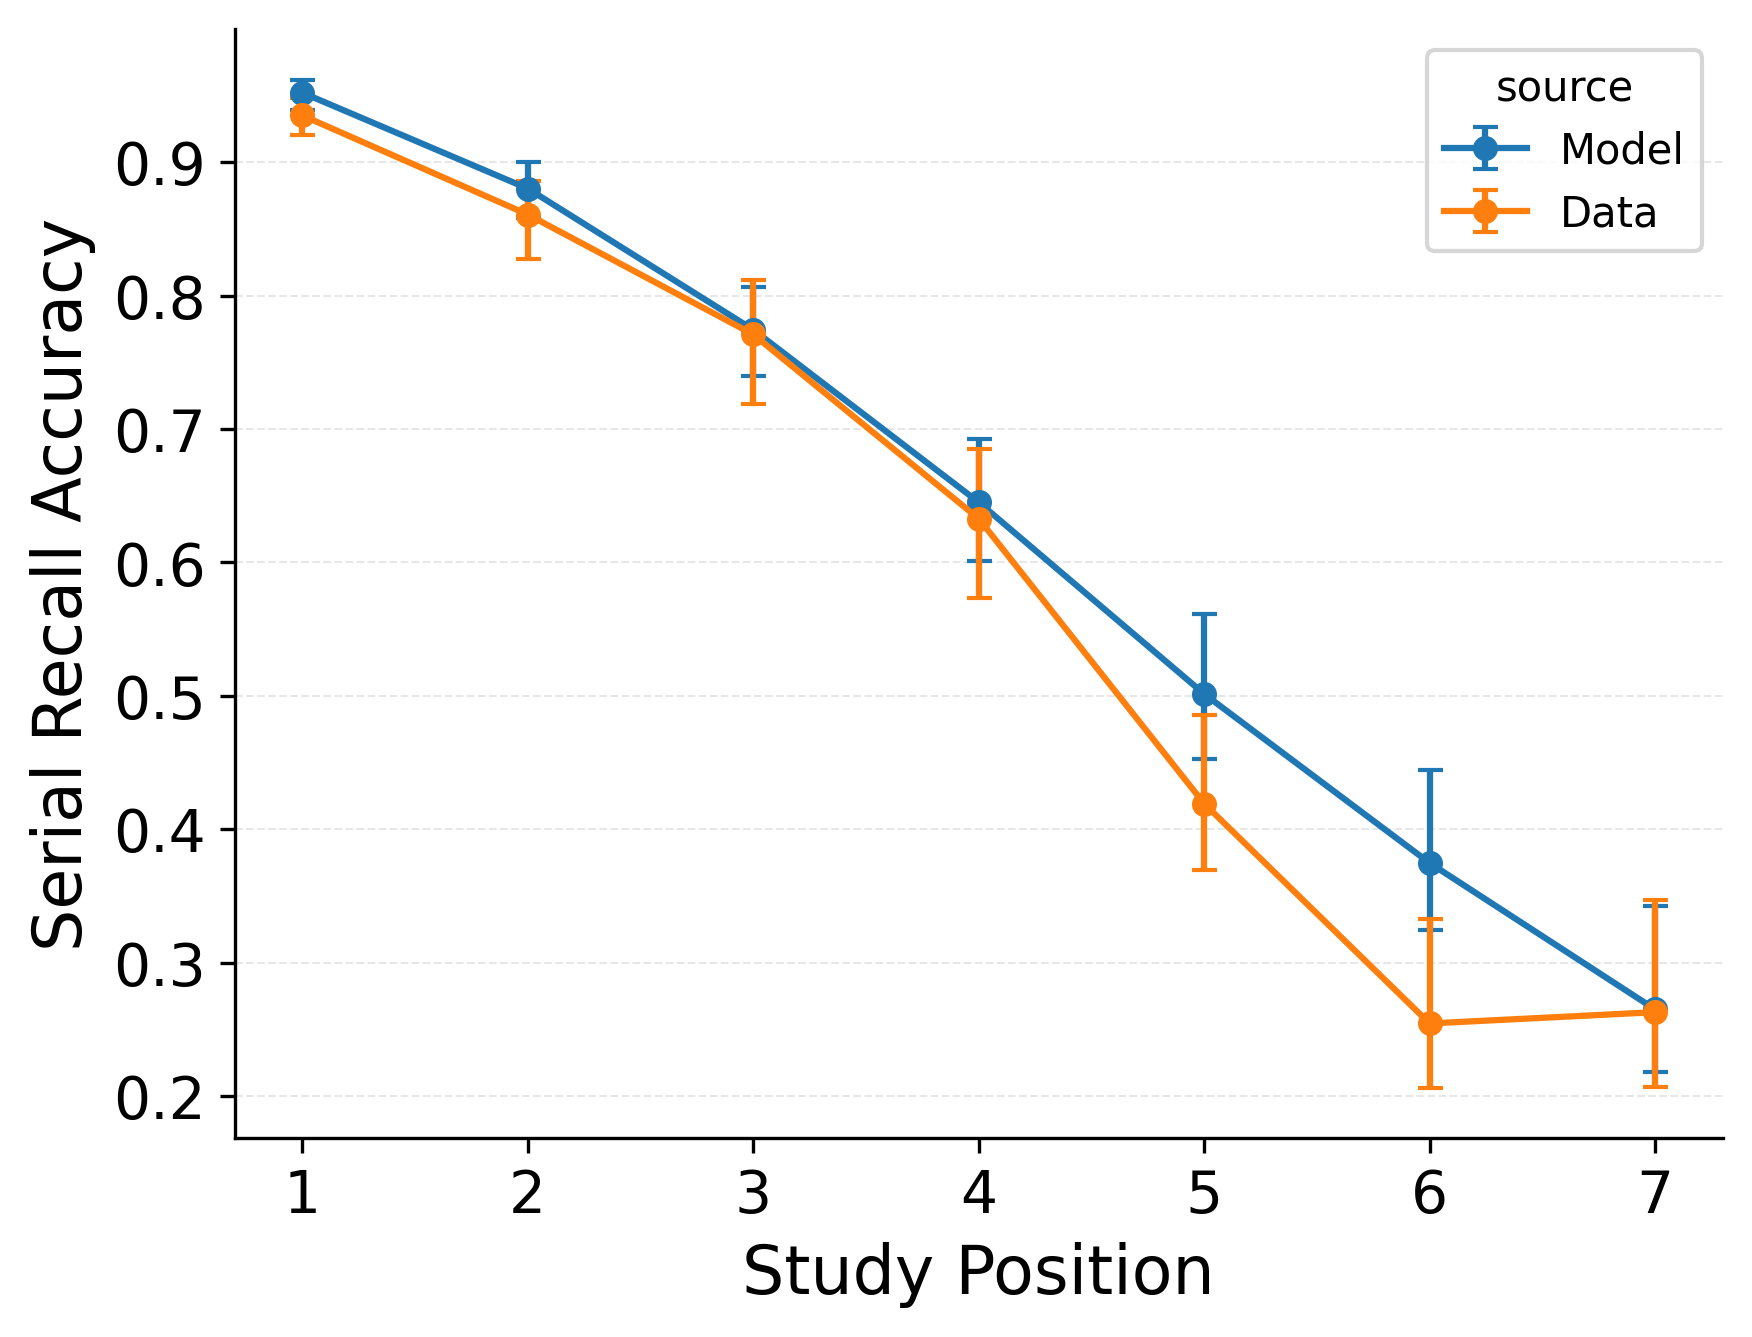
\includegraphics{figures/Gordon2021_CRU_with_Pre-Expt_and_Primacy__and_ContextTerm_Confusable_Fitting_srac_LL7.png}\end{minipage}%
\newline
\begin{minipage}{0.33\linewidth}
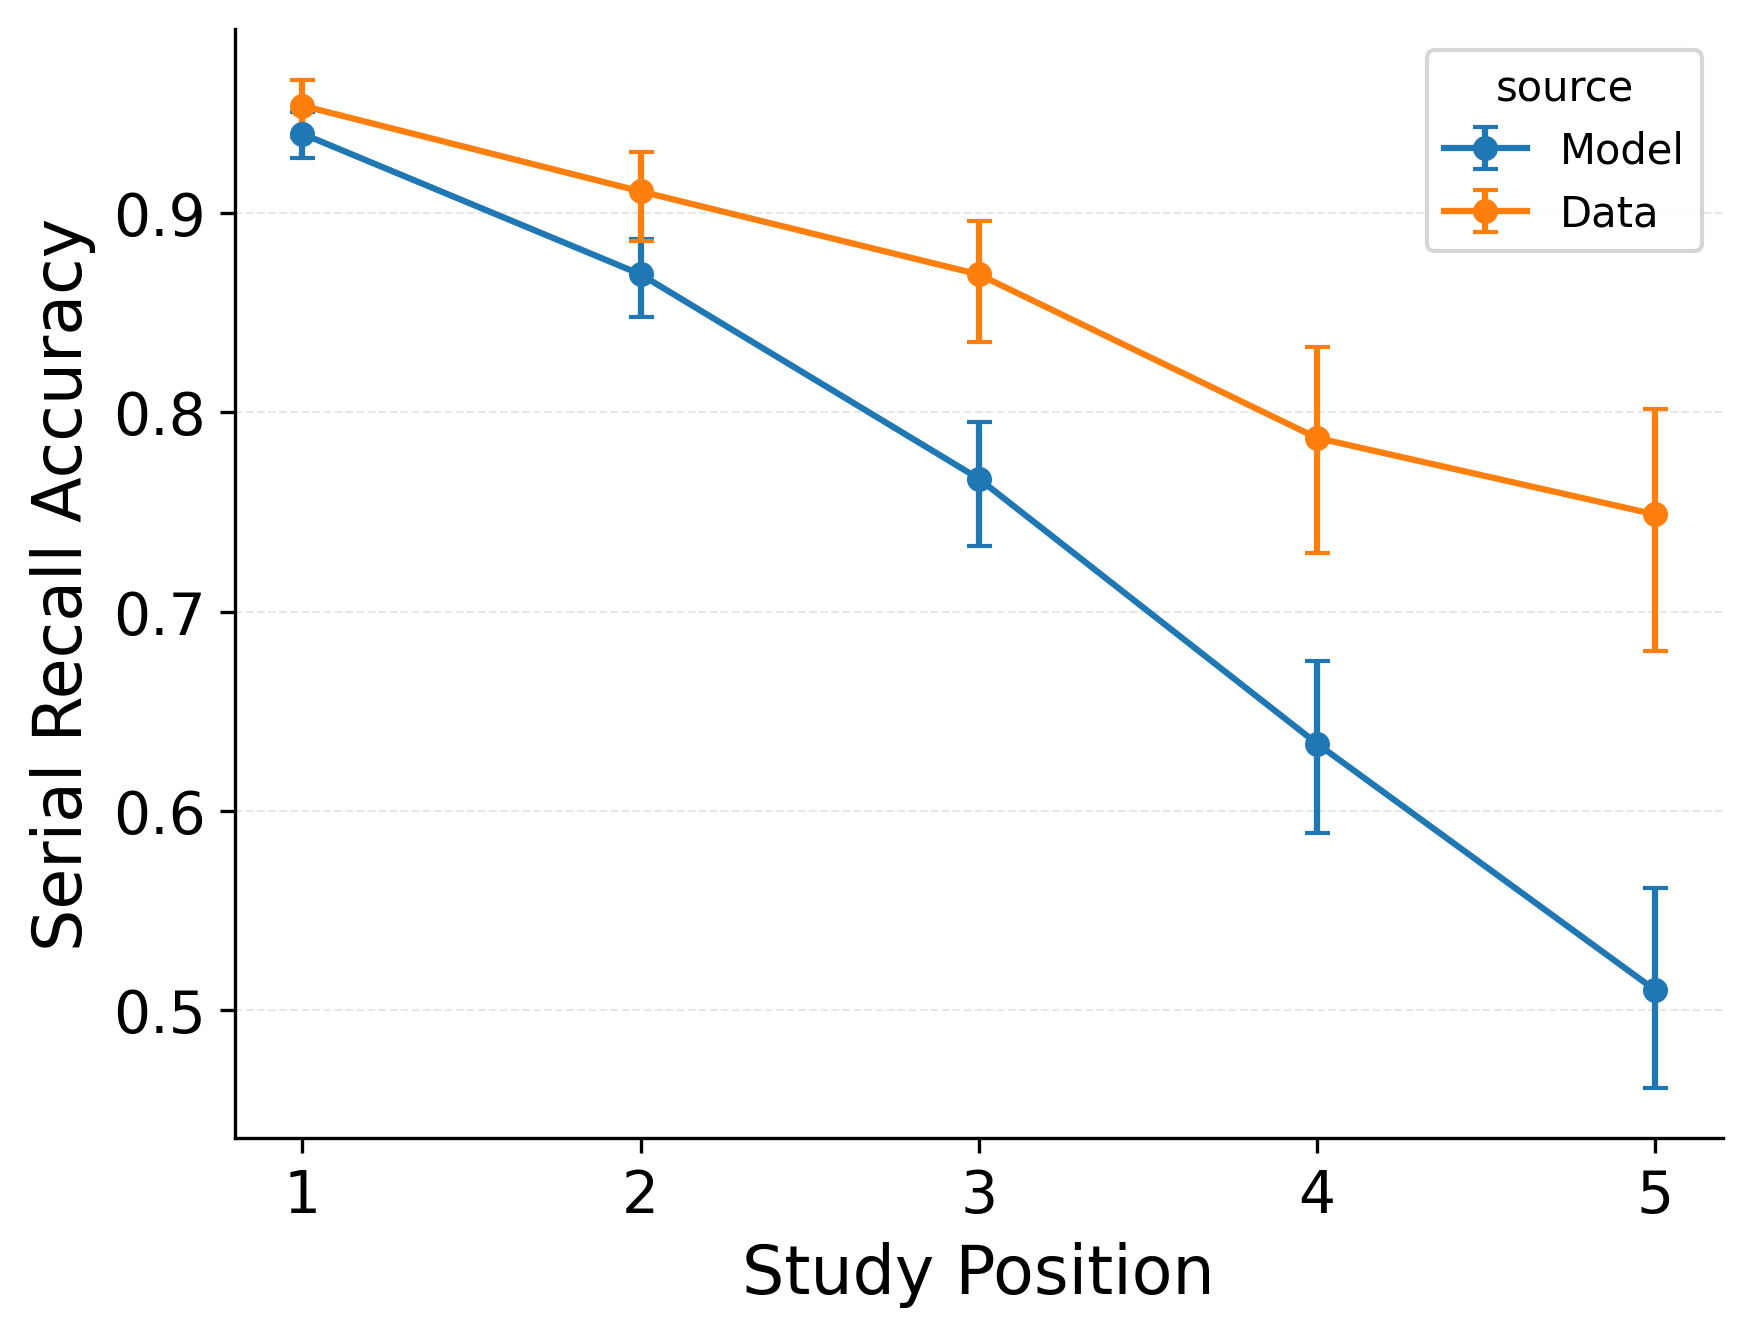
\includegraphics{figures/Gordon2021_BaseCMR_Confusable_Fitting_srac_LL5.png}\end{minipage}%
%
\begin{minipage}{0.33\linewidth}
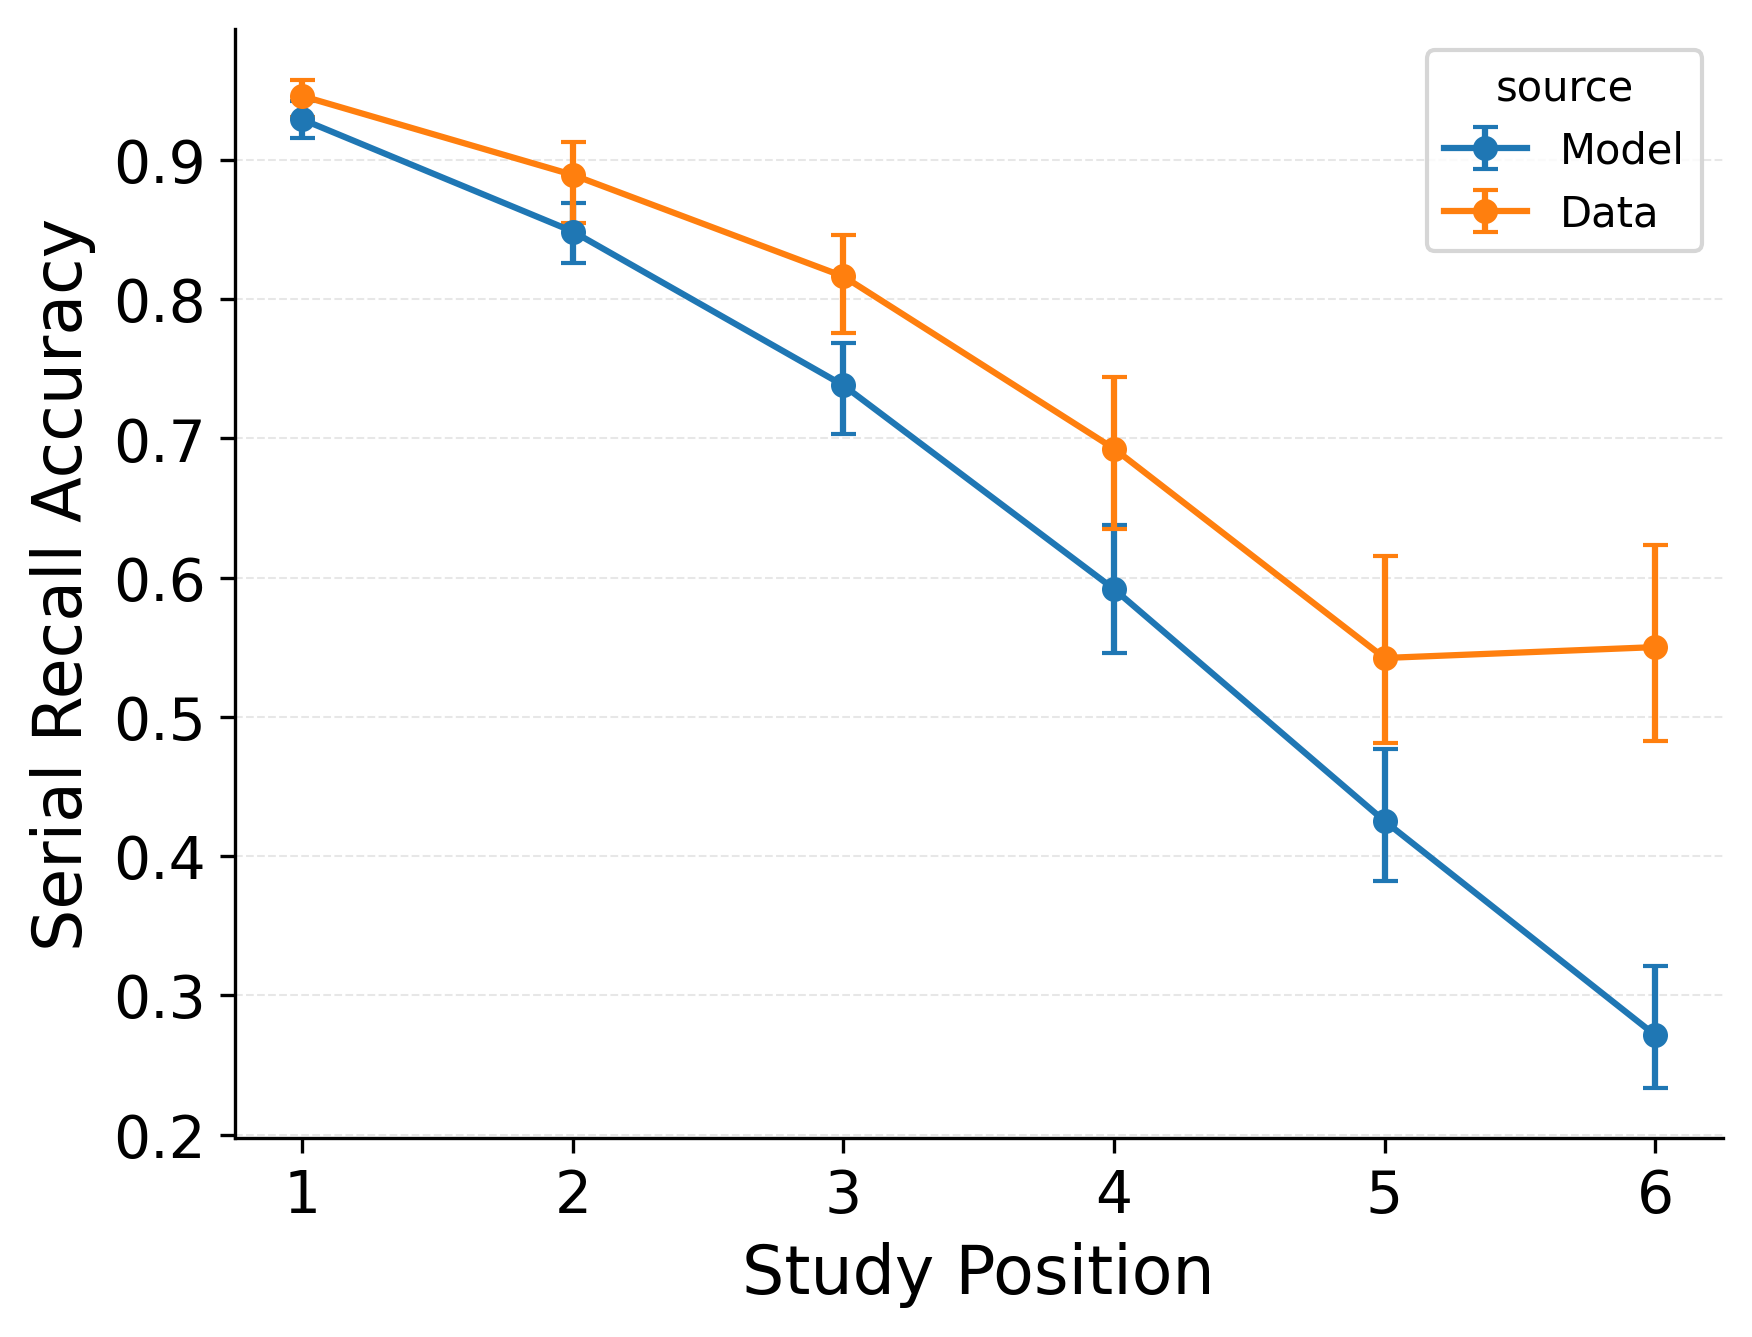
\includegraphics{figures/Gordon2021_BaseCMR_Confusable_Fitting_srac_LL6.png}\end{minipage}%
%
\begin{minipage}{0.33\linewidth}
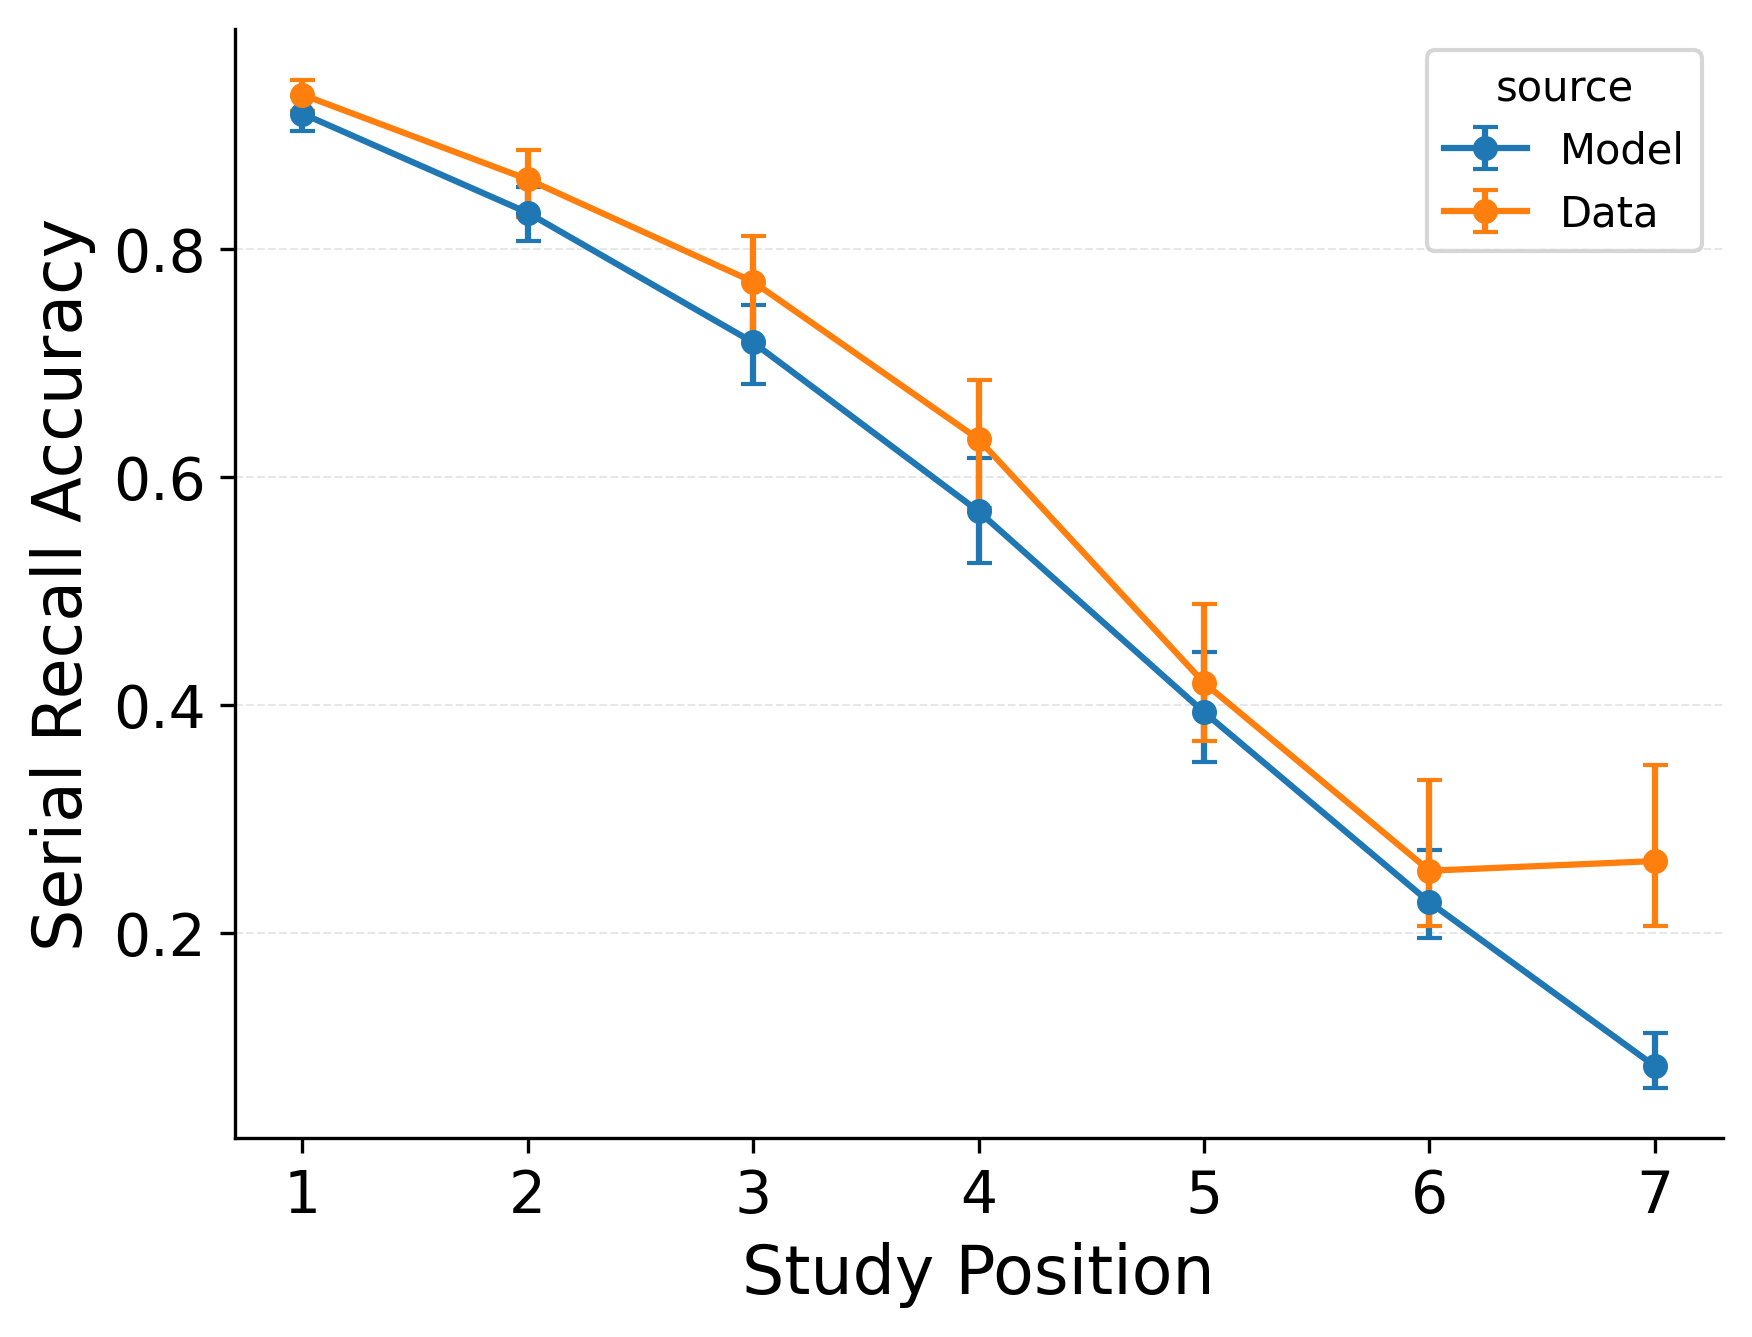
\includegraphics{figures/Gordon2021_BaseCMR_Confusable_Fitting_srac_LL7.png}\end{minipage}%

\end{figure}%

\begin{figure}

\caption{\label{fig-best-serial-errors}Intrusion, order, and omission
error rates (top, middle, and bottom rows respectively) by serial
position for list lengths 5, 6, and 7 (left, center, and right columns),
in Logan (\citeproc{ref-logan2021serial}{2021}) serial recall data.
Lines compare observed error rates with predicted error rates from best
performing CRU variant with free pre-experimental context-to-feature
memory (\(\alpha\), \(\delta\)) and CMR-specific primacy gradient
(\(\phi_\text{s}\), \(\phi_\text{d}\)) parameters.}

\begin{minipage}{0.33\linewidth}
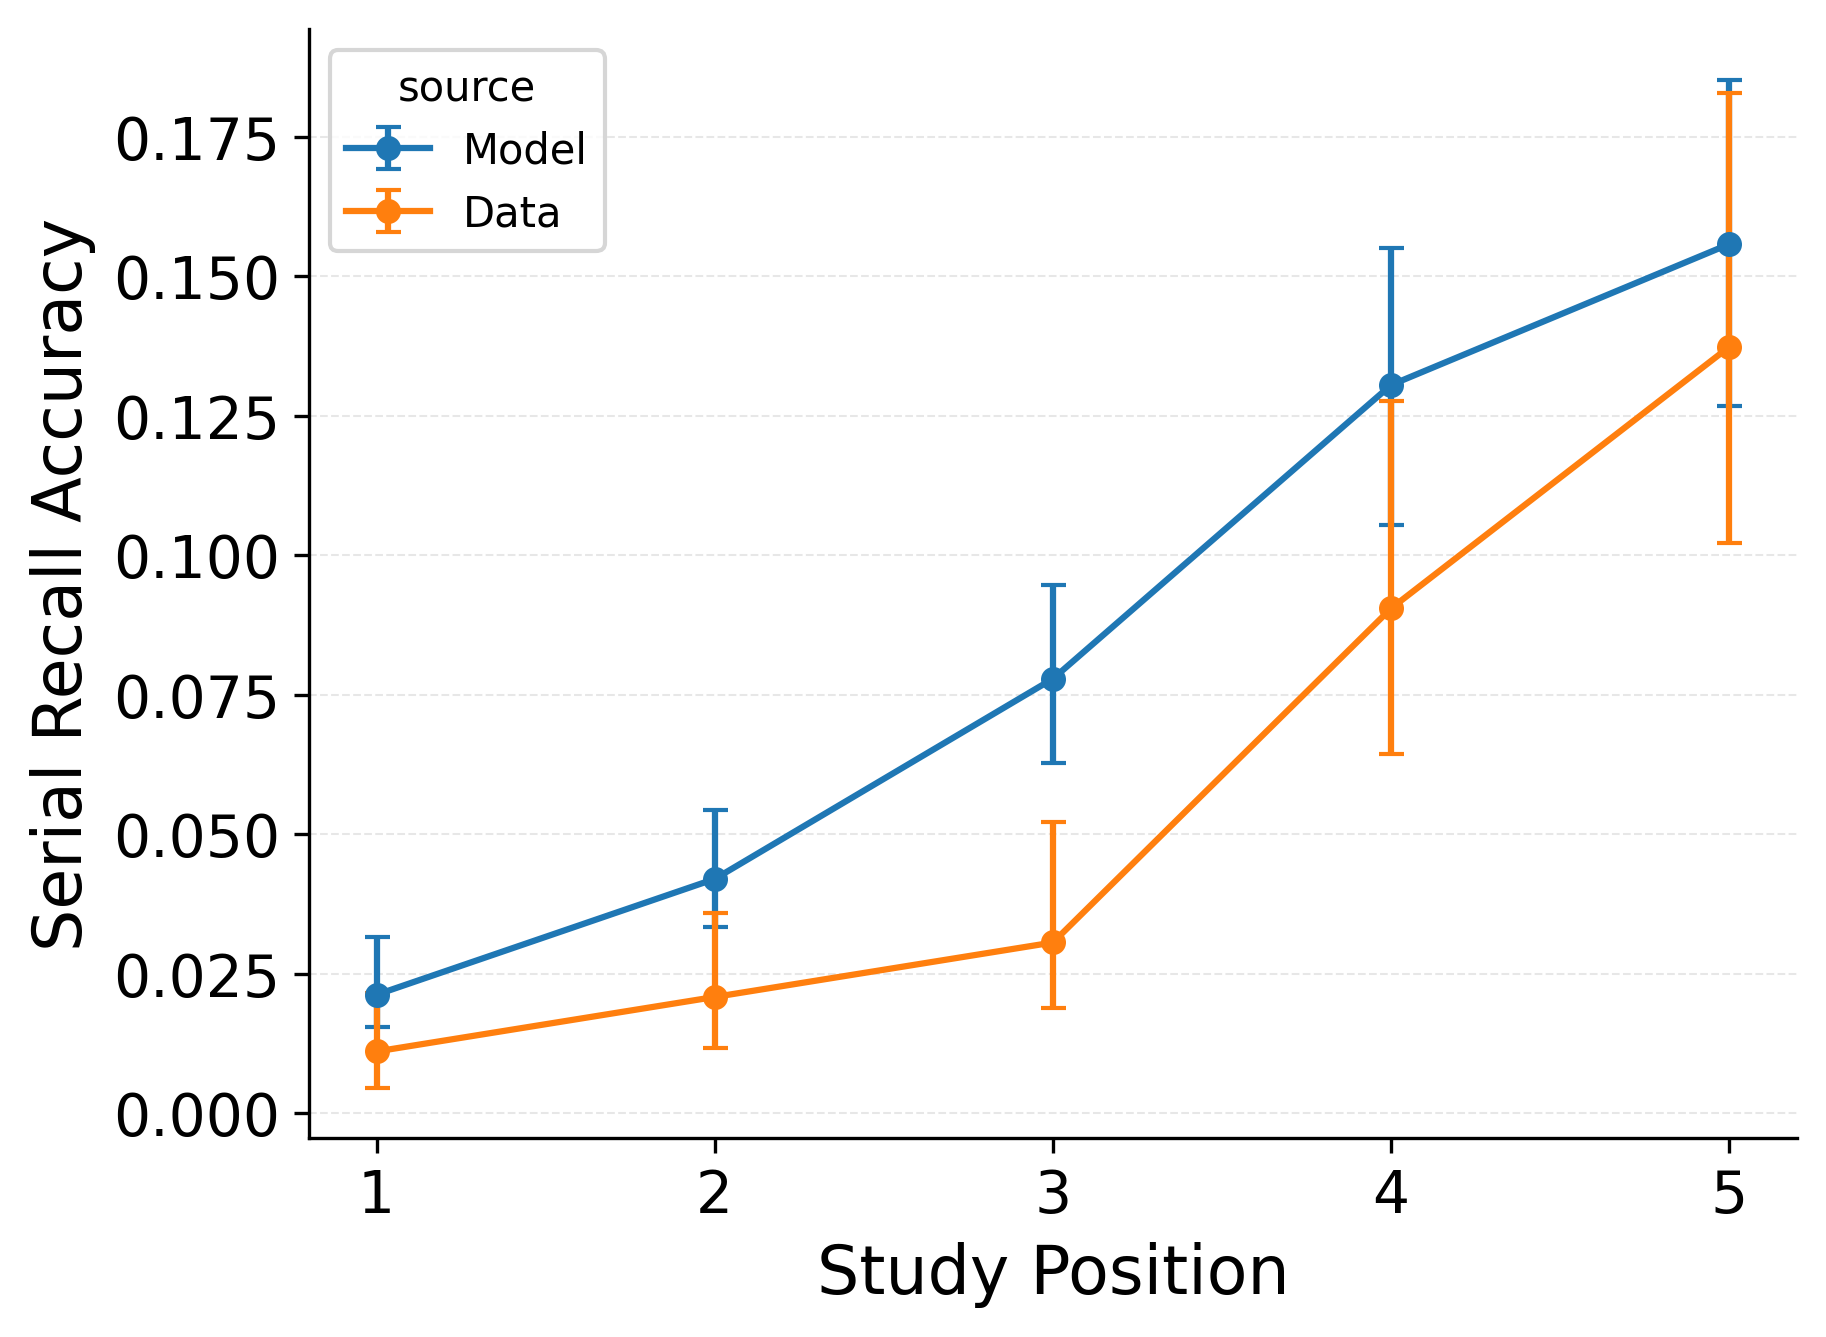
\includegraphics{figures/Gordon2021_CRU_with_Pre-Expt_and_Primacy__and_ContextTerm_Confusable_Fitting_intrusion_error_rate_LL5.png}\end{minipage}%
%
\begin{minipage}{0.33\linewidth}
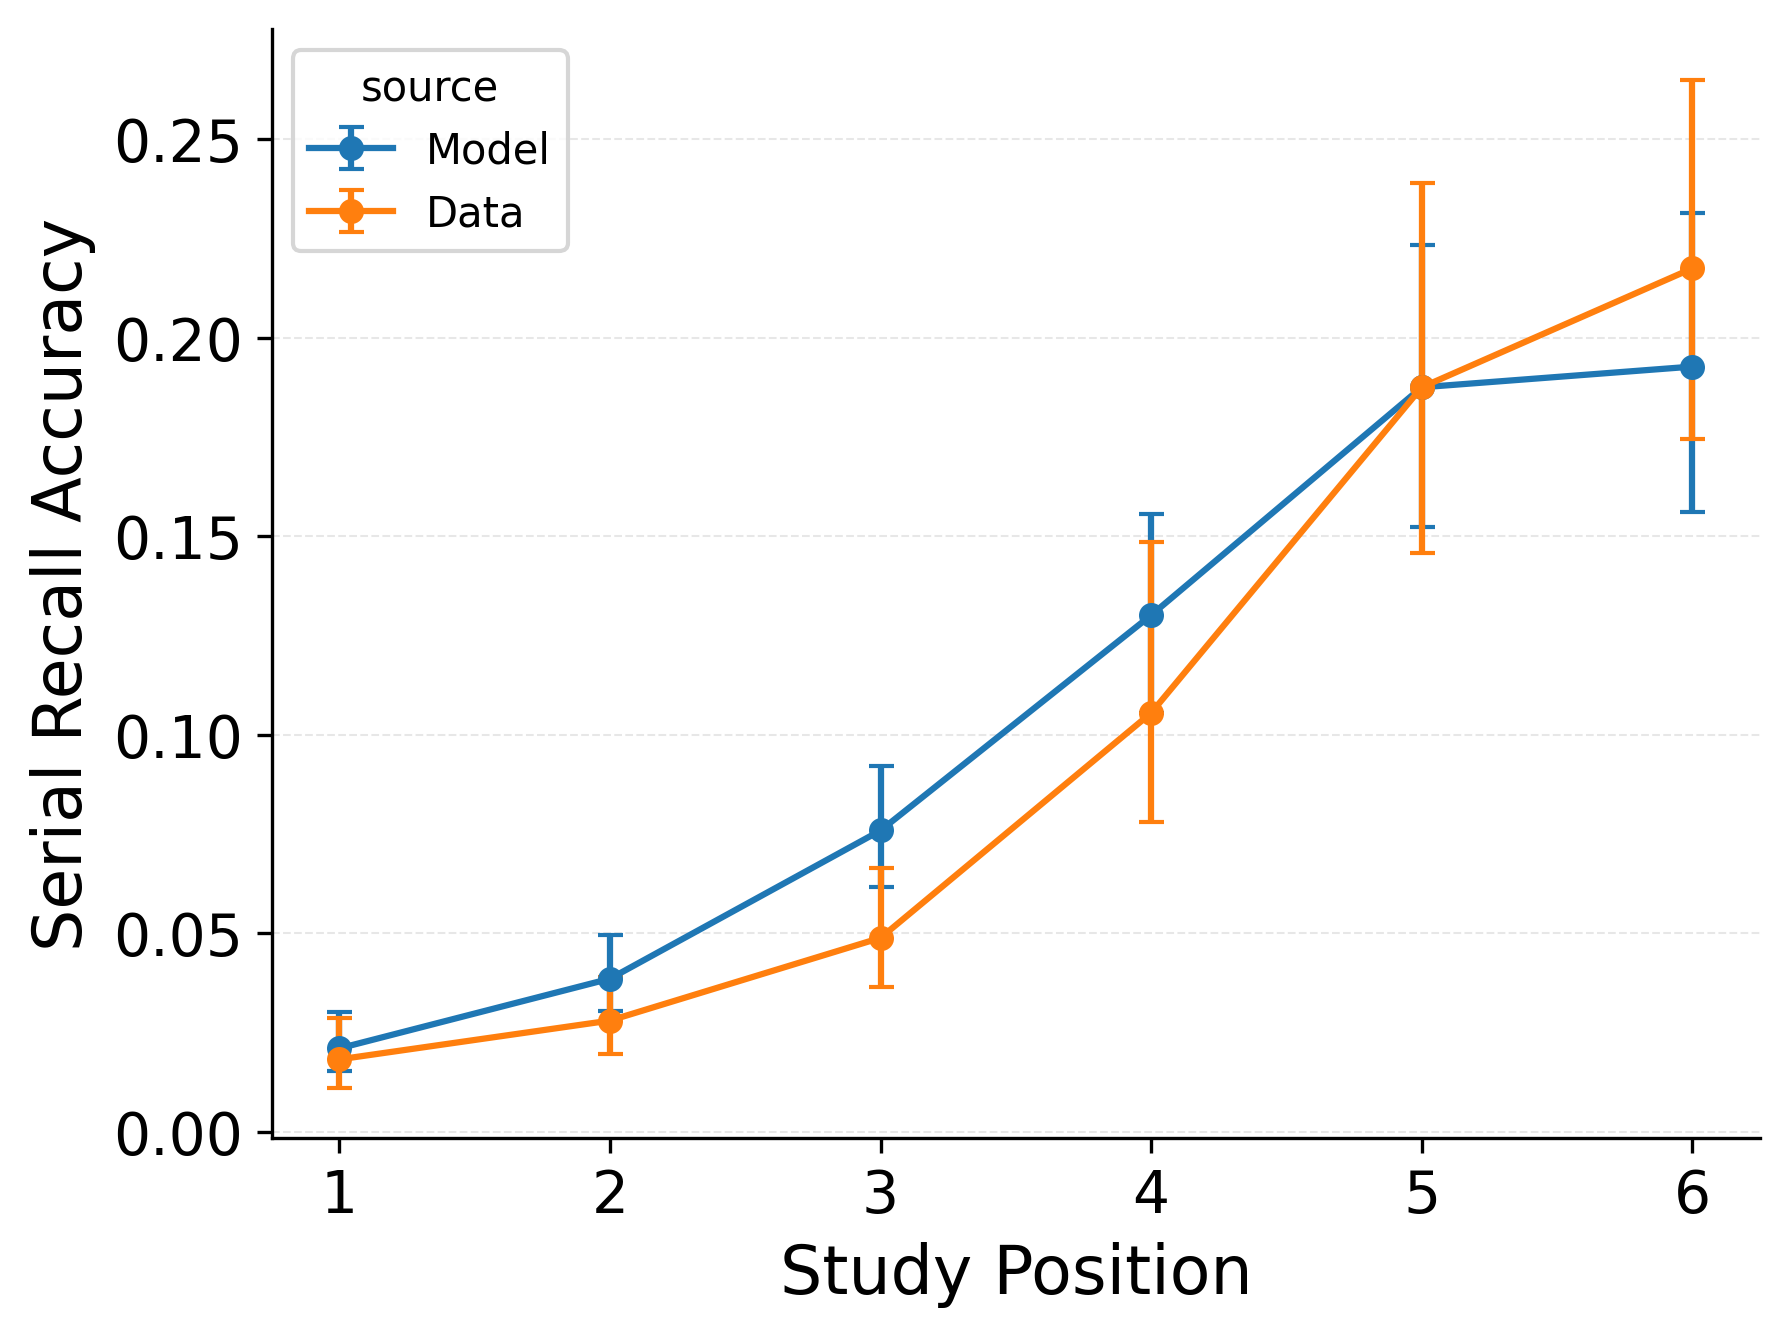
\includegraphics{figures/Gordon2021_CRU_with_Pre-Expt_and_Primacy__and_ContextTerm_Confusable_Fitting_intrusion_error_rate_LL6.png}\end{minipage}%
%
\begin{minipage}{0.33\linewidth}
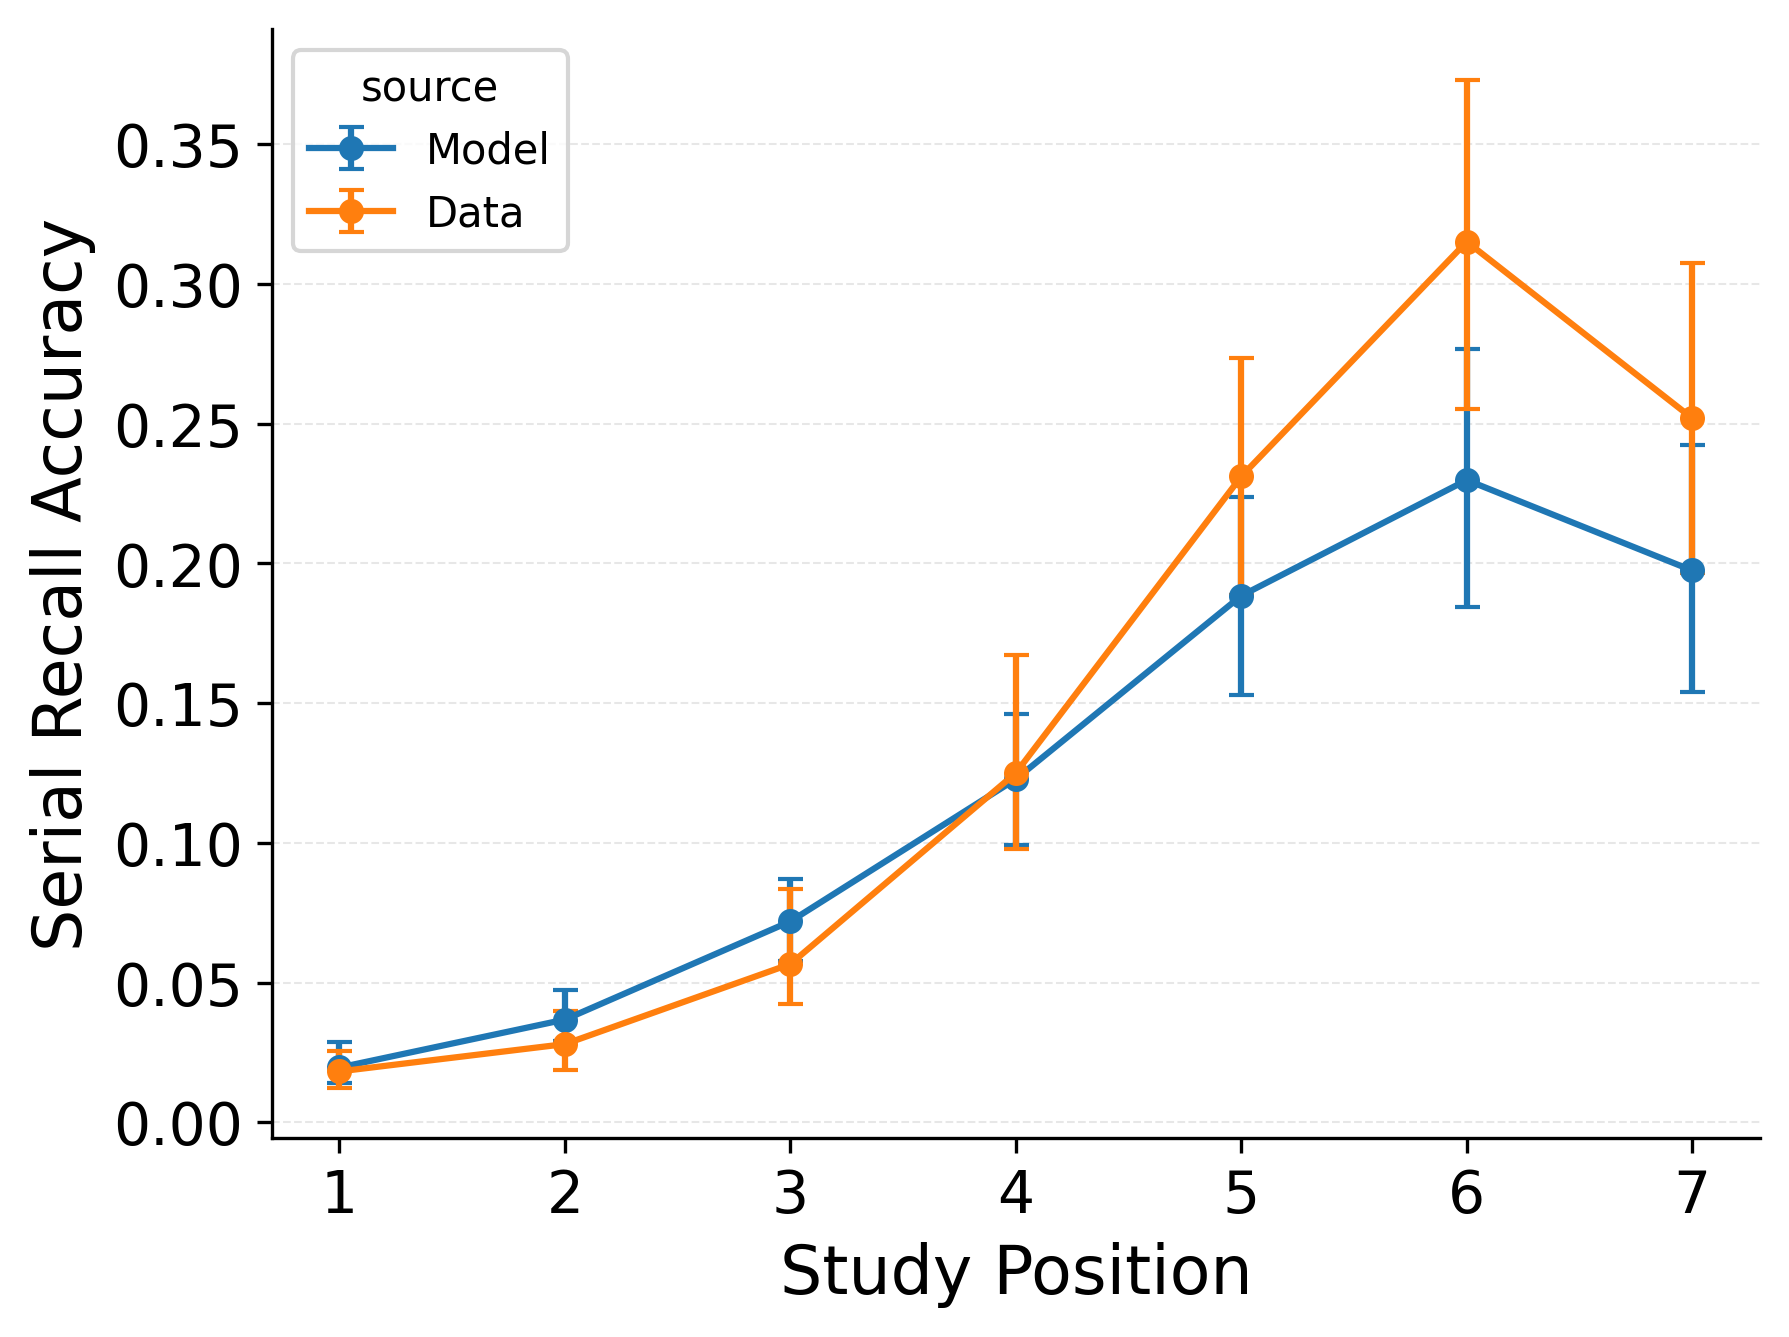
\includegraphics{figures/Gordon2021_CRU_with_Pre-Expt_and_Primacy__and_ContextTerm_Confusable_Fitting_intrusion_error_rate_LL7.png}\end{minipage}%
\newline
\begin{minipage}{0.33\linewidth}
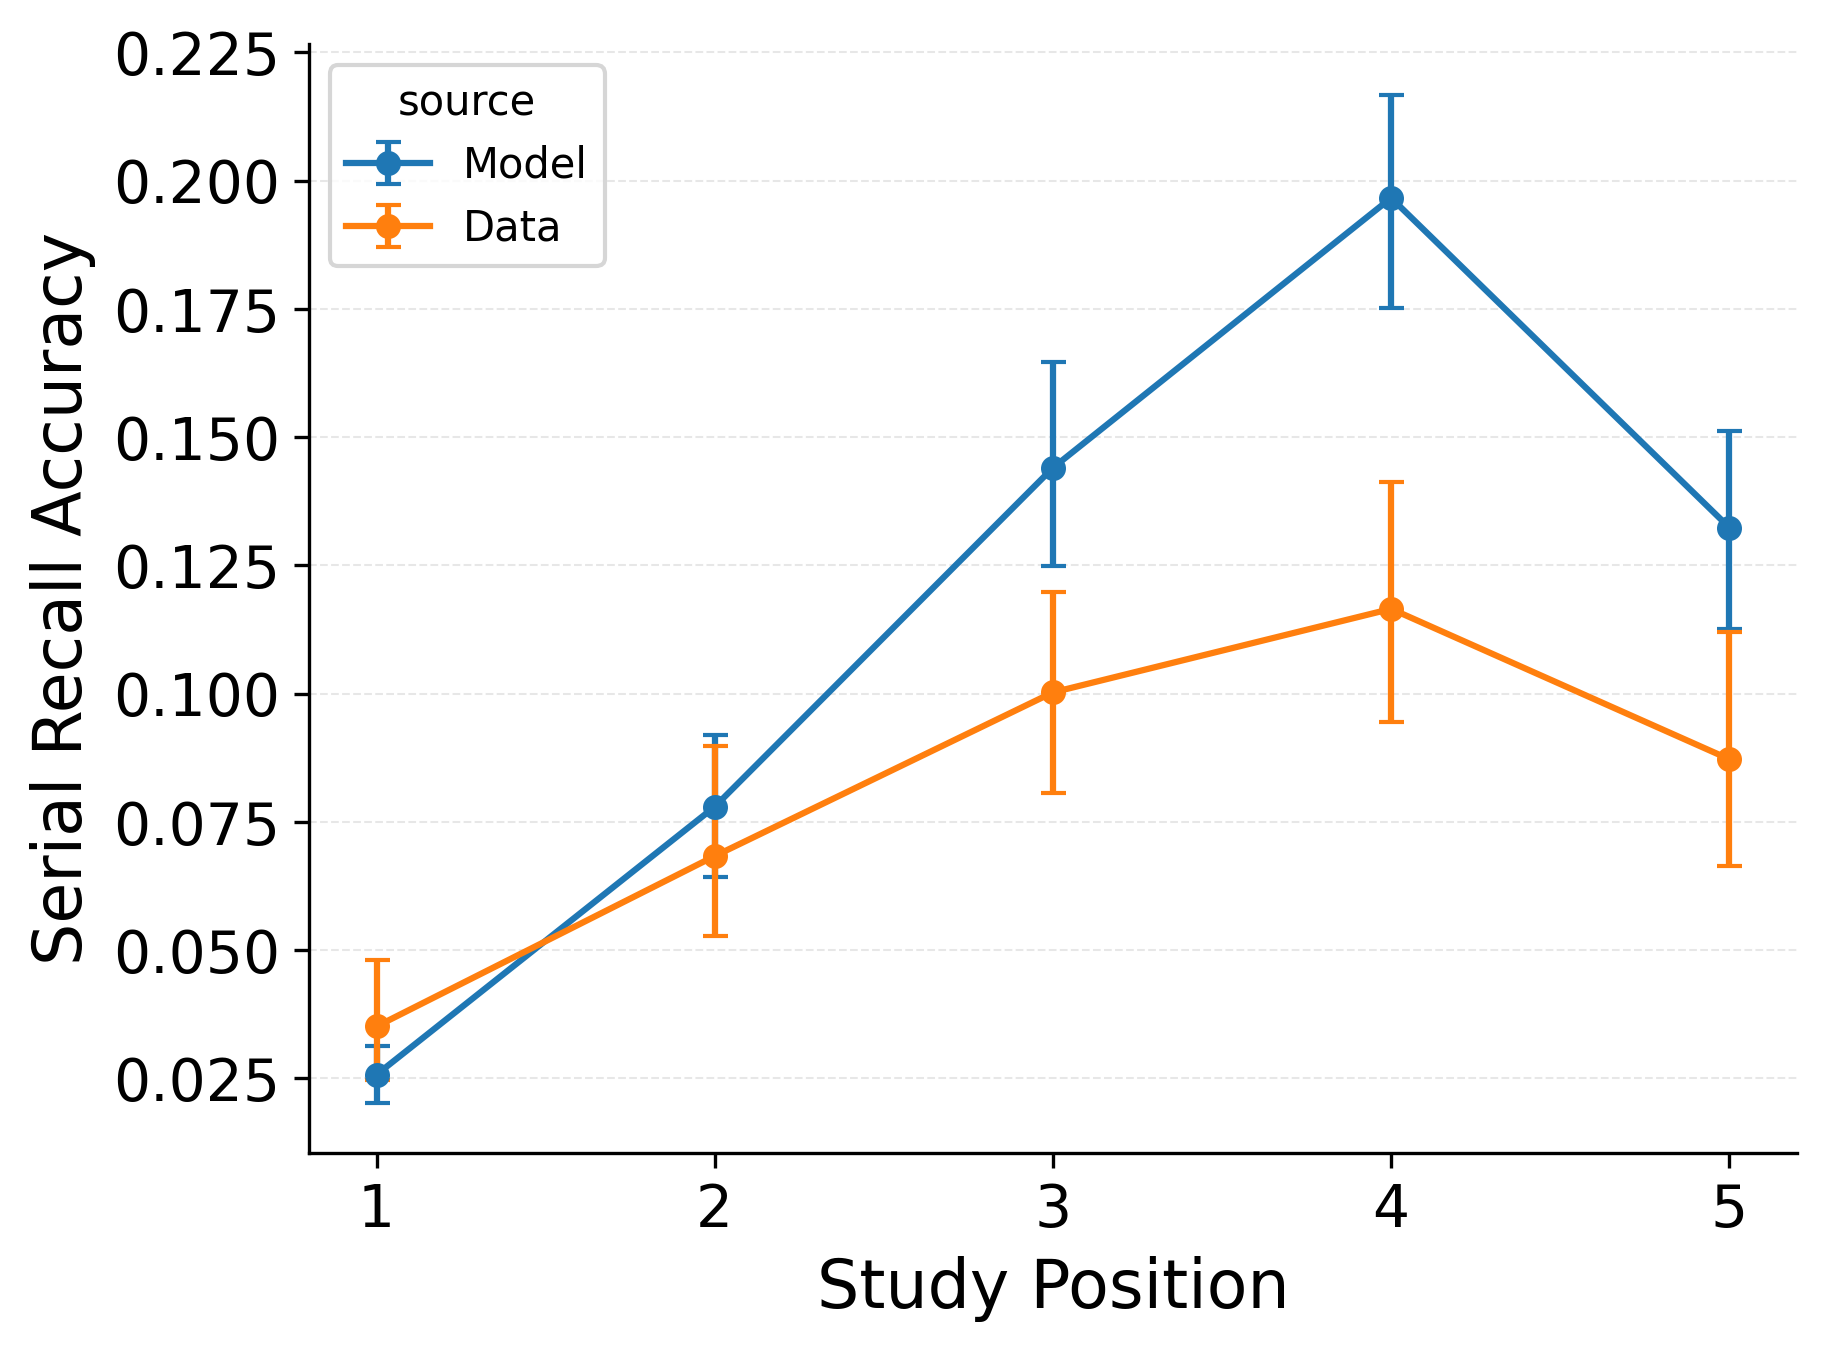
\includegraphics{figures/Gordon2021_CRU_with_Pre-Expt_and_Primacy__and_ContextTerm_Confusable_Fitting_order_error_rate_LL5.png}\end{minipage}%
%
\begin{minipage}{0.33\linewidth}
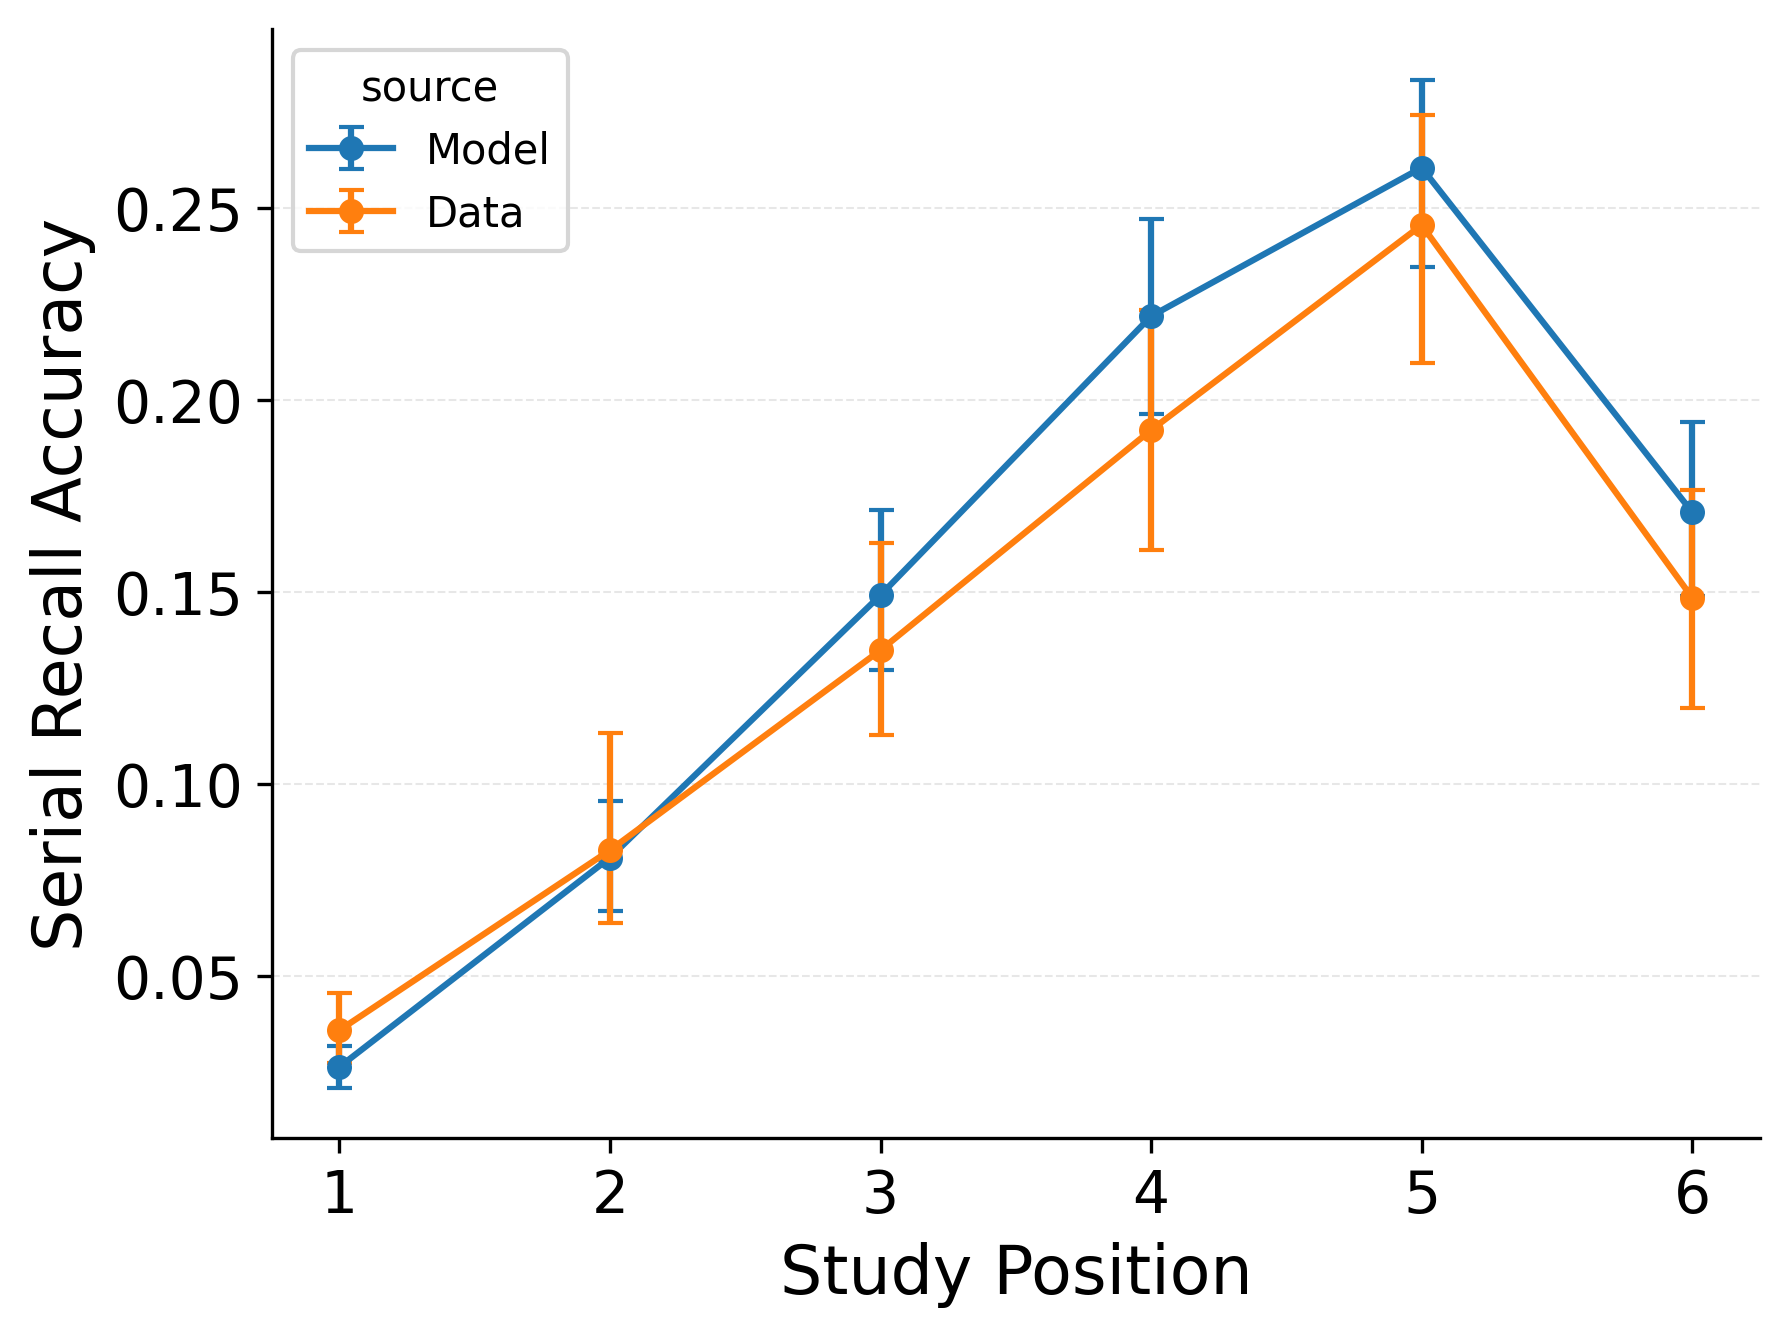
\includegraphics{figures/Gordon2021_CRU_with_Pre-Expt_and_Primacy__and_ContextTerm_Confusable_Fitting_order_error_rate_LL6.png}\end{minipage}%
%
\begin{minipage}{0.33\linewidth}
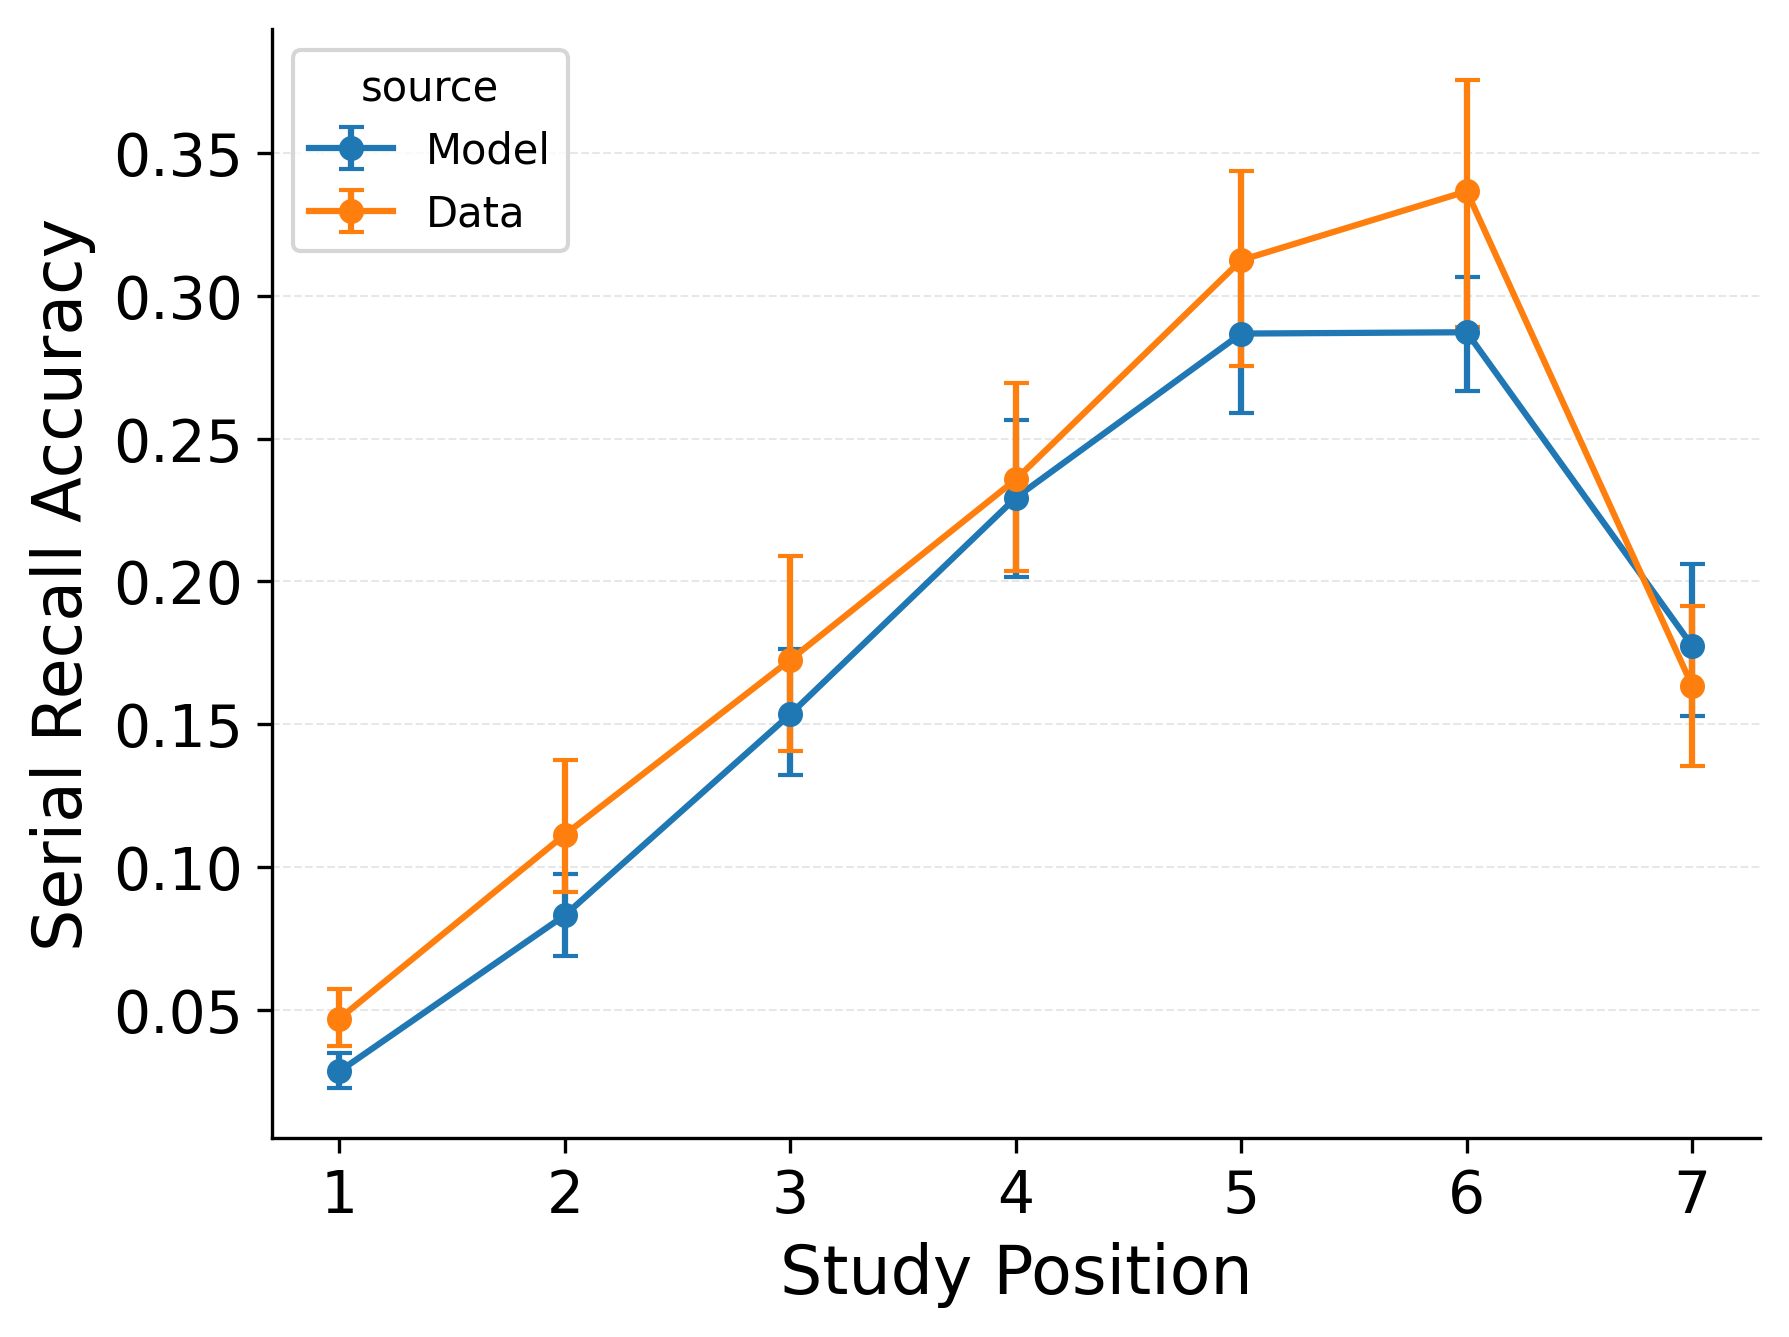
\includegraphics{figures/Gordon2021_CRU_with_Pre-Expt_and_Primacy__and_ContextTerm_Confusable_Fitting_order_error_rate_LL7.png}\end{minipage}%
\newline
\begin{minipage}{0.33\linewidth}
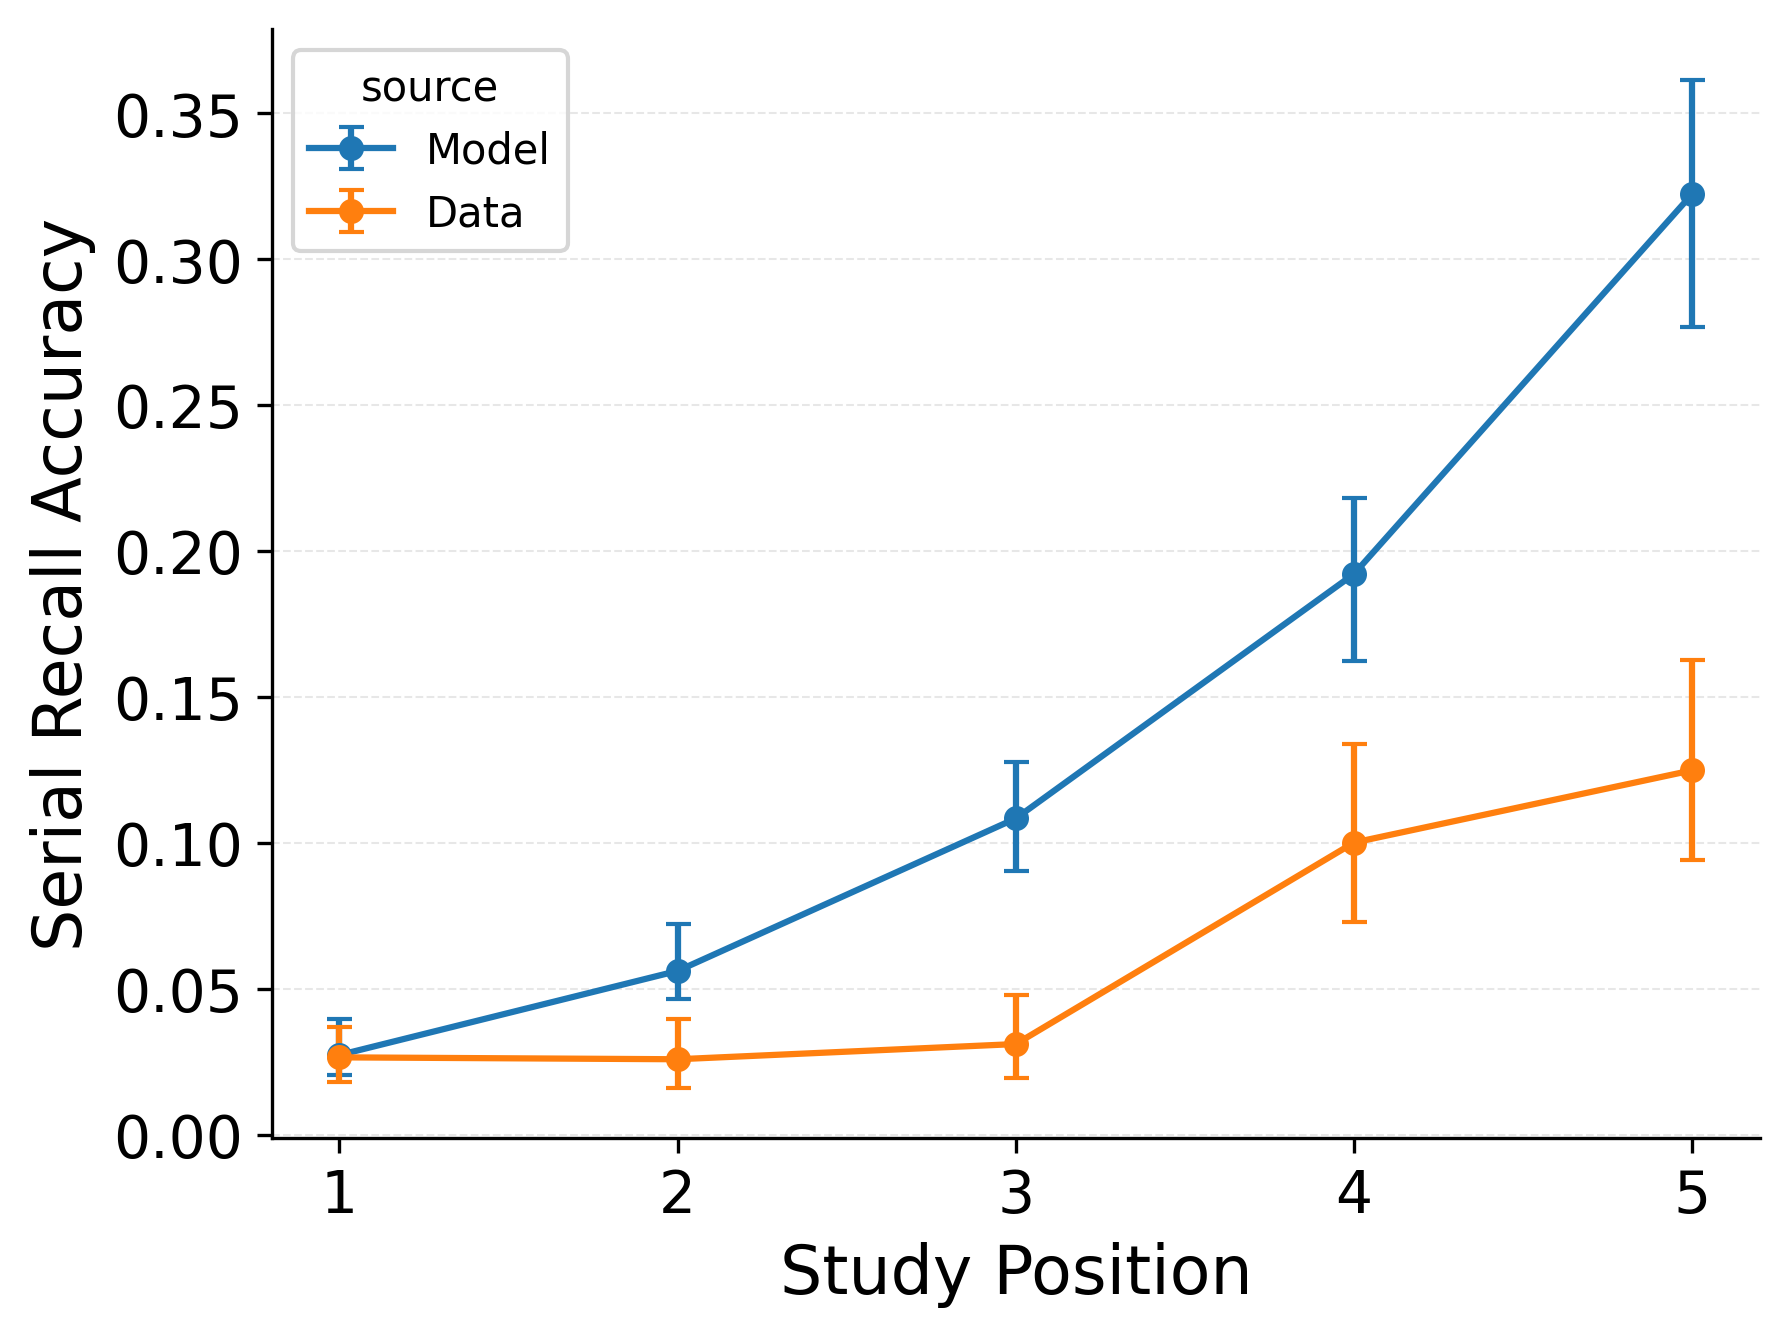
\includegraphics{figures/Gordon2021_CRU_with_Pre-Expt_and_Primacy__and_ContextTerm_Confusable_Fitting_omission_error_rate_LL5.png}\end{minipage}%
%
\begin{minipage}{0.33\linewidth}
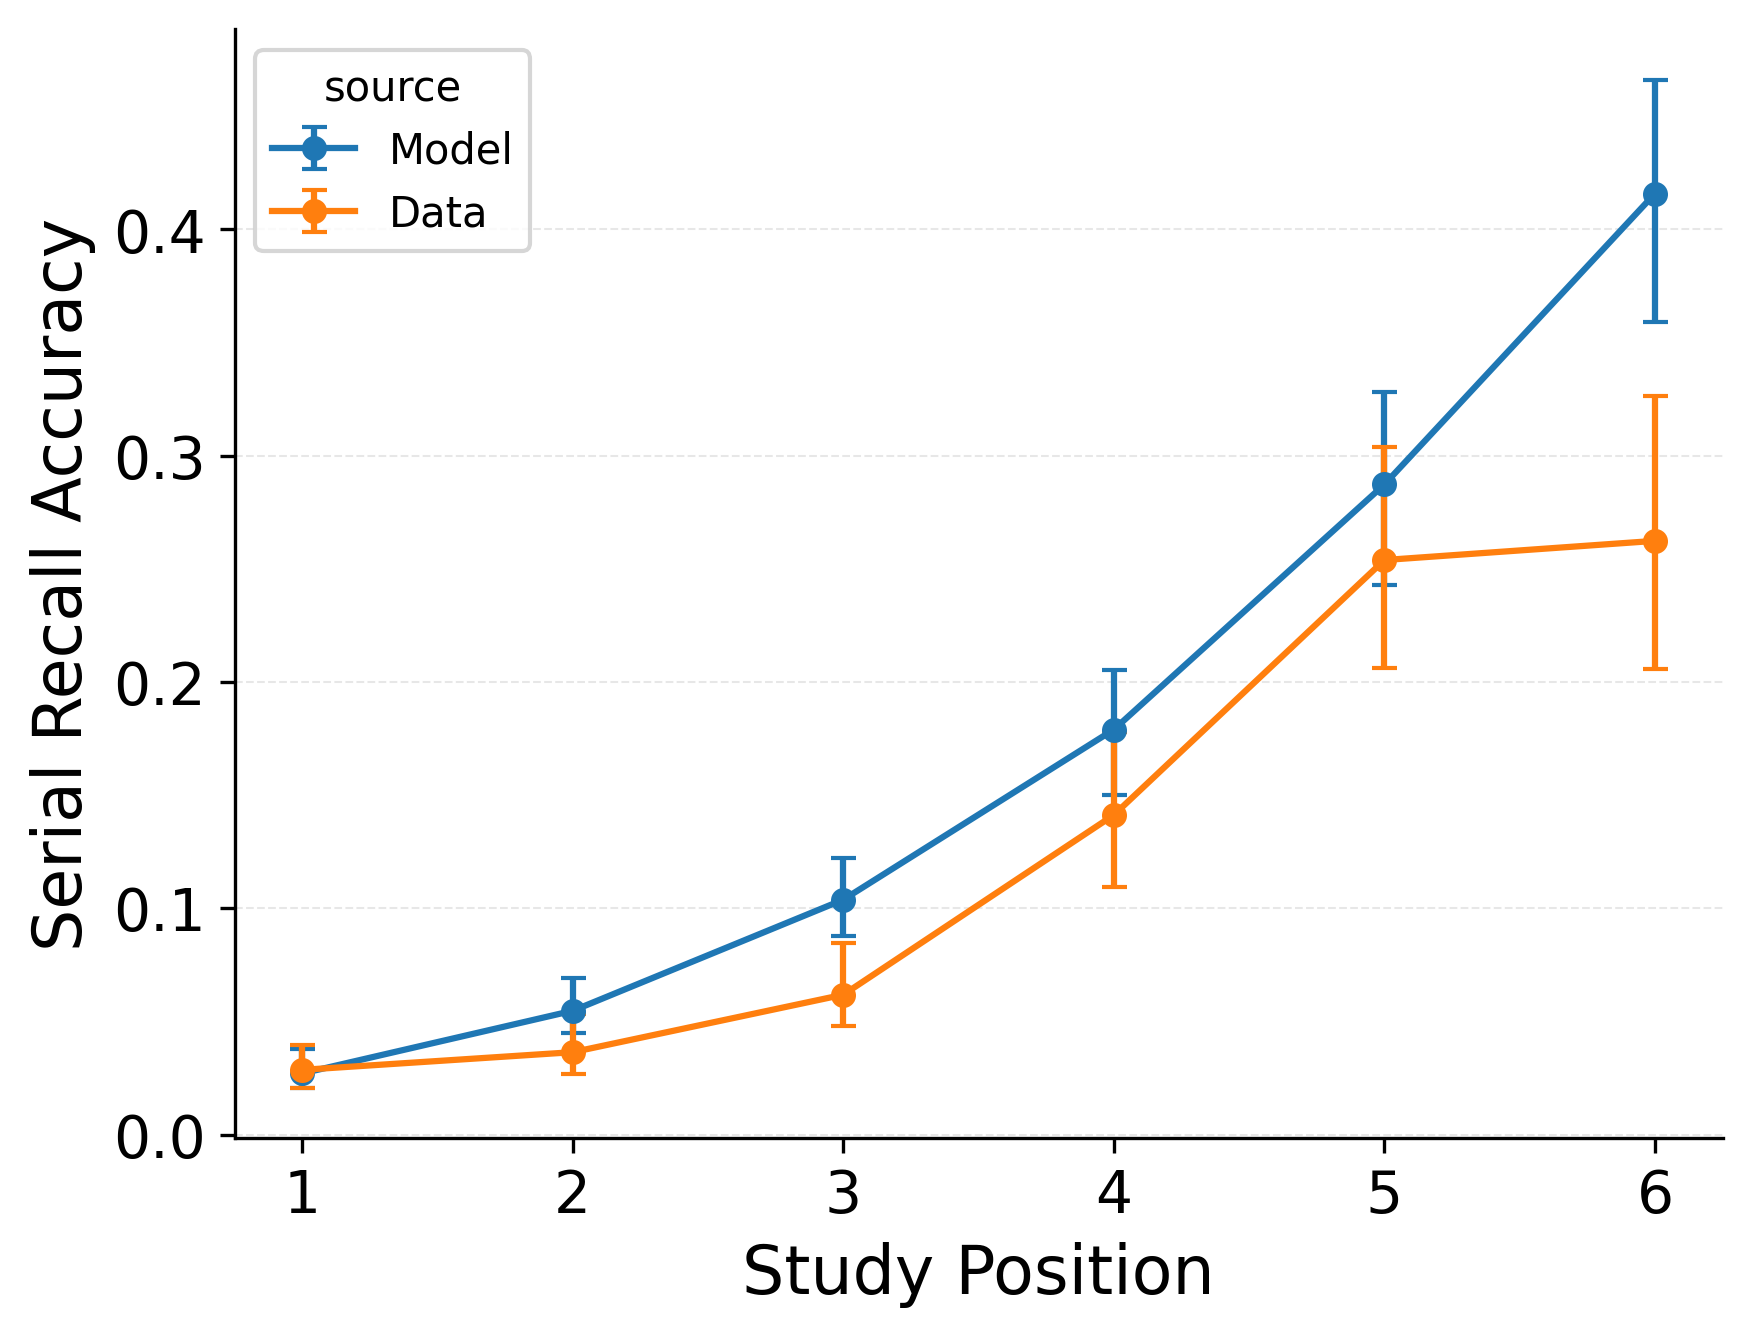
\includegraphics{figures/Gordon2021_CRU_with_Pre-Expt_and_Primacy__and_ContextTerm_Confusable_Fitting_omission_error_rate_LL6.png}\end{minipage}%
%
\begin{minipage}{0.33\linewidth}
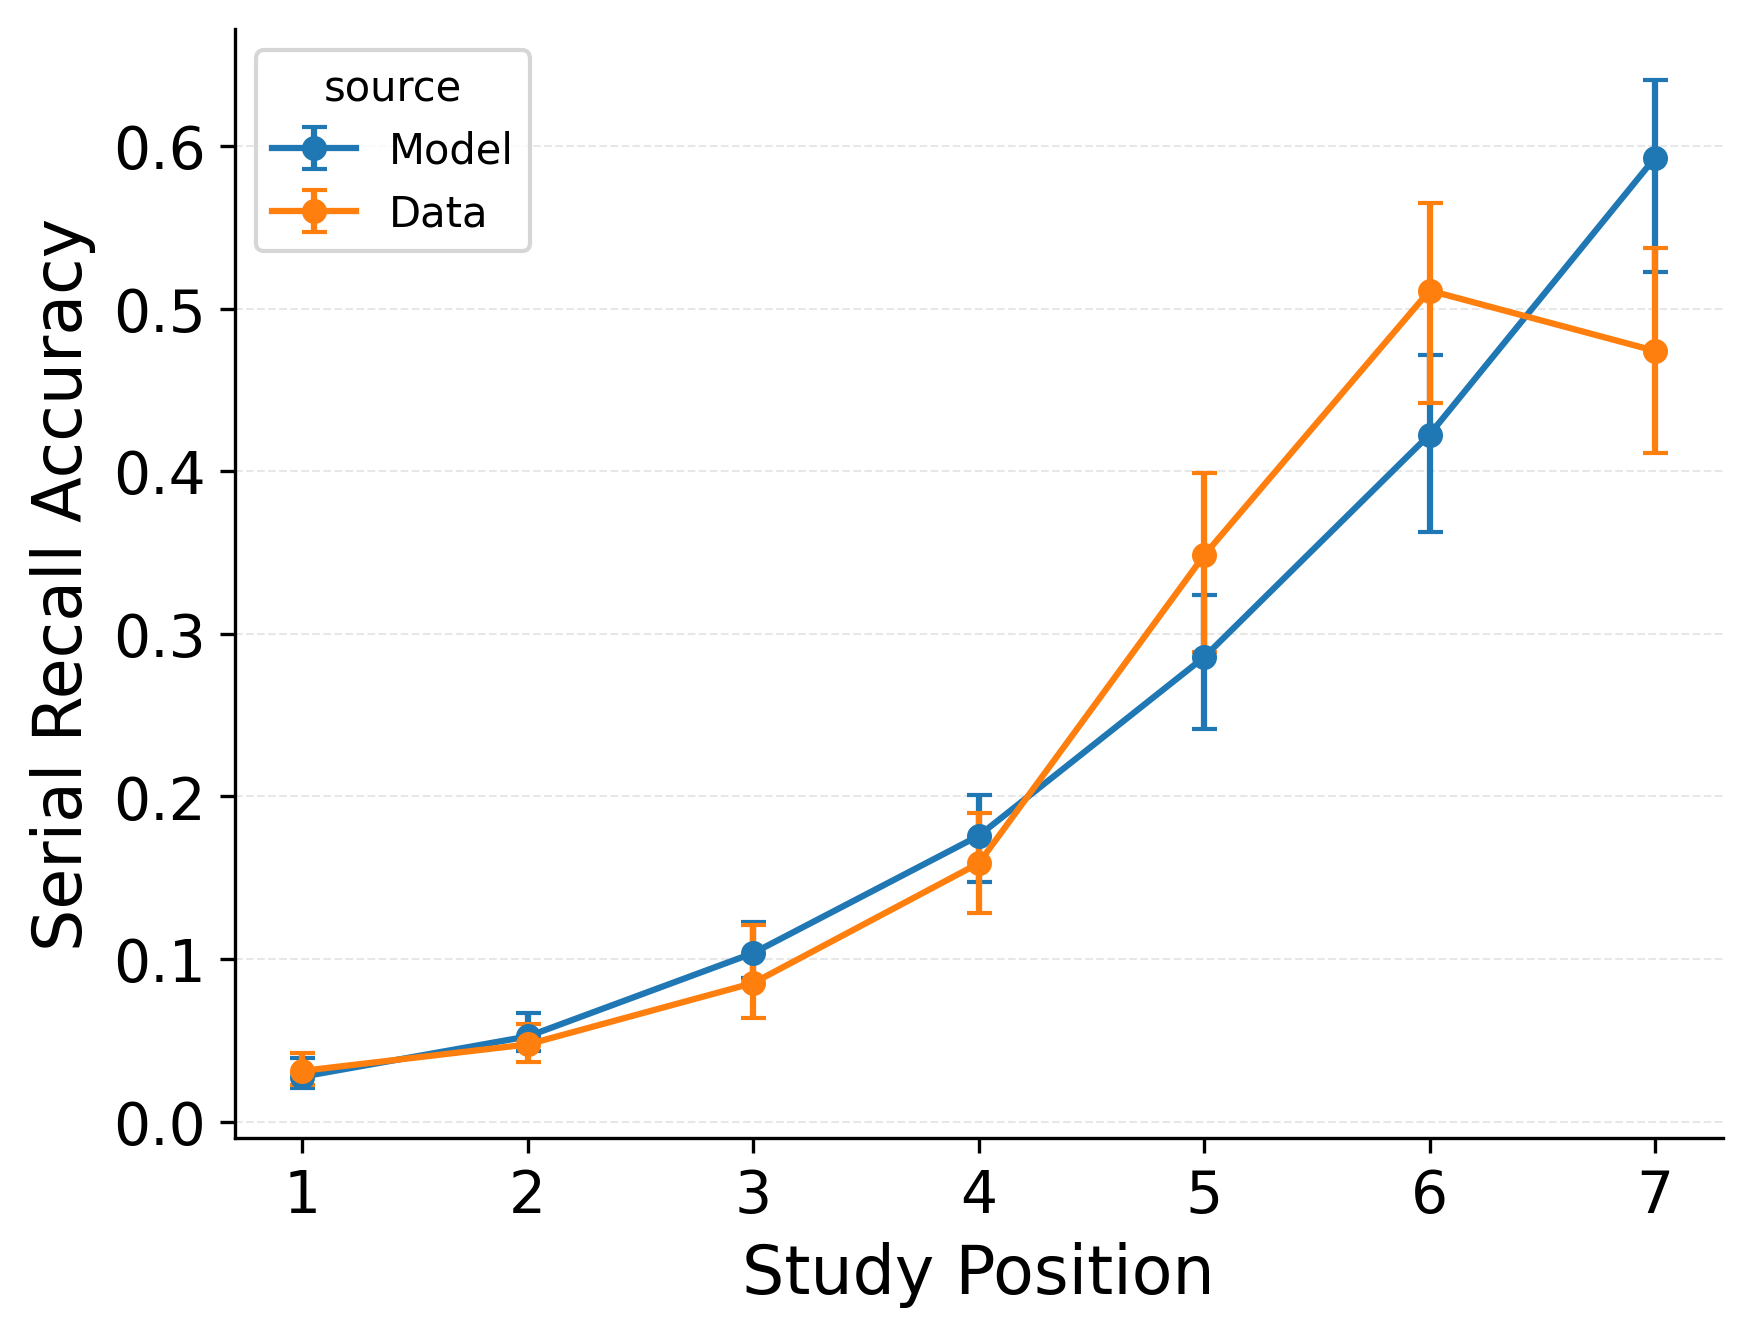
\includegraphics{figures/Gordon2021_CRU_with_Pre-Expt_and_Primacy__and_ContextTerm_Confusable_Fitting_omission_error_rate_LL7.png}\end{minipage}%

\end{figure}%

In serial recall, participants generally initiate with the first item of
the list and rarely exploit recency to guide retrieval. This is seen in
the serial recall accuracy curves of Figure~\ref{fig-serial-srac}, which
measure how often a participant recalls the correct item in the correct
output position (a more stringent measure than the serial position
analysis of free recall). Performance starts high and declines steadily
across serial positions.

CRU has multiple mechanisms that support this primacy effect in serial
recall performance. CRU always initiates recall using the start-of-list
context (equivalent to CMR's \(\beta_\text{start}\) = 1.0), and this
context is always most associated with the first item in the list.
Likewise, CRU's pre-existing encoding contextual drift gradient
(\(\beta_\text{dec}\)) also provide a strong primacy gradient to boost
recall accuracy for early-list items. Finally, the letter-identification
gradient (higher confusability toward the end of the list) causes better
performance in earlier positions than later positions. Correspondingly,
CRU fits the serial recall accuracy curves well, as shown in
Figure~\ref{fig-serial-srac} (top row). Enabling CMR's associative
primacy gradient (\(\phi_\text{s}\), \(\phi_\text{d}\)) and
pre-experimental context-to-feature memory (\(\alpha\), \(\delta\))
parameters improves the model's overall fit to the data substantially,
but this improvement is not clearly seen in the serial recall accuracy
analysis Figure~\ref{fig-serial-srac}, where fits only improve slightly.

These outcomes reproduce prior results showing that CMR mechanisms
needed to balance primacy and recency in free recall become less
important in serial recall when the task enforces a fixed forward order
(\citeproc{ref-logan2021serial}{Logan, 2021};
\citeproc{ref-lohnas2024retrieved}{Lohnas, 2024}). Because strict serial
recall requires reproducing items from the start, it is not necessary to
manipulate the \(\beta_\text{start}\) parameter downward from its
already maximal value of 1.

CRU also explains how different types of response errors are distributed
across serial positions. Logan (\citeproc{ref-logan2021serial}{2021})
characterized and simulated three types of errors. Order errors occur
when a participant recalls an item from the list but in the wrong
position. Intrusion errors occur when a participant recalls an item that
was not on the list. Finally, omission errors occur when a participant
fails to recall an item that was on the list. Rates of all three types
of errors generally increase as a function of serial position in the
Logan (\citeproc{ref-logan2021serial}{2021}) dataset. Importantly,
intrusion errors are captured by CRU's item identification confusability
mechanism. Since CRU can address serial recall accuracy and error
patterns without CMR's additional mechanisms, a variant of CMR that
drops its pre-existing primacy gradient mechanisms in favor of CRU's
confusability mechanism could prove a more parsimonious model of memory
search across free and serial recall if the mechanism can be extended to
capture confusion rates for words. Figure~\ref{fig-best-serial-errors}
shows the predicted and observed rates of intrusion, order, and omission
errors by serial position for the best performing CRU variant with free
pre-experimental context-to-feature memory (\(\alpha\), \(\delta\)) and
CMR-specific primacy gradient (\(\phi_\text{s}\), \(\phi_\text{d}\))
parameters.

\subsection{Forward and Backward Transitions in Serial
Recall}\label{forward-and-backward-transitions-in-serial-recall}

\begin{figure}

\caption{\label{fig-serial-crp}Lag-conditional response probability
(lag-CRP) fits of baseline CRU (\textbf{Top}); best performing CRU
variant with free pre-experimental context-to-feature memory
(\(\alpha\), \(\delta\)) and CMR-specific primacy gradient
(\(\phi_\text{s}\), \(\phi_\text{d}\)) parameters (\textbf{Middle}); and
CMR with its default position-based recall termination mechanism and
CRU's item identification confusability mechanism (\textbf{Bottom}) to
Logan (\citeproc{ref-logan2021serial}{2021}) serial recall data. Lines
compare observed lag-CRP with predicted lag-CRP for the applicable model
variant.}

\begin{minipage}{0.33\linewidth}
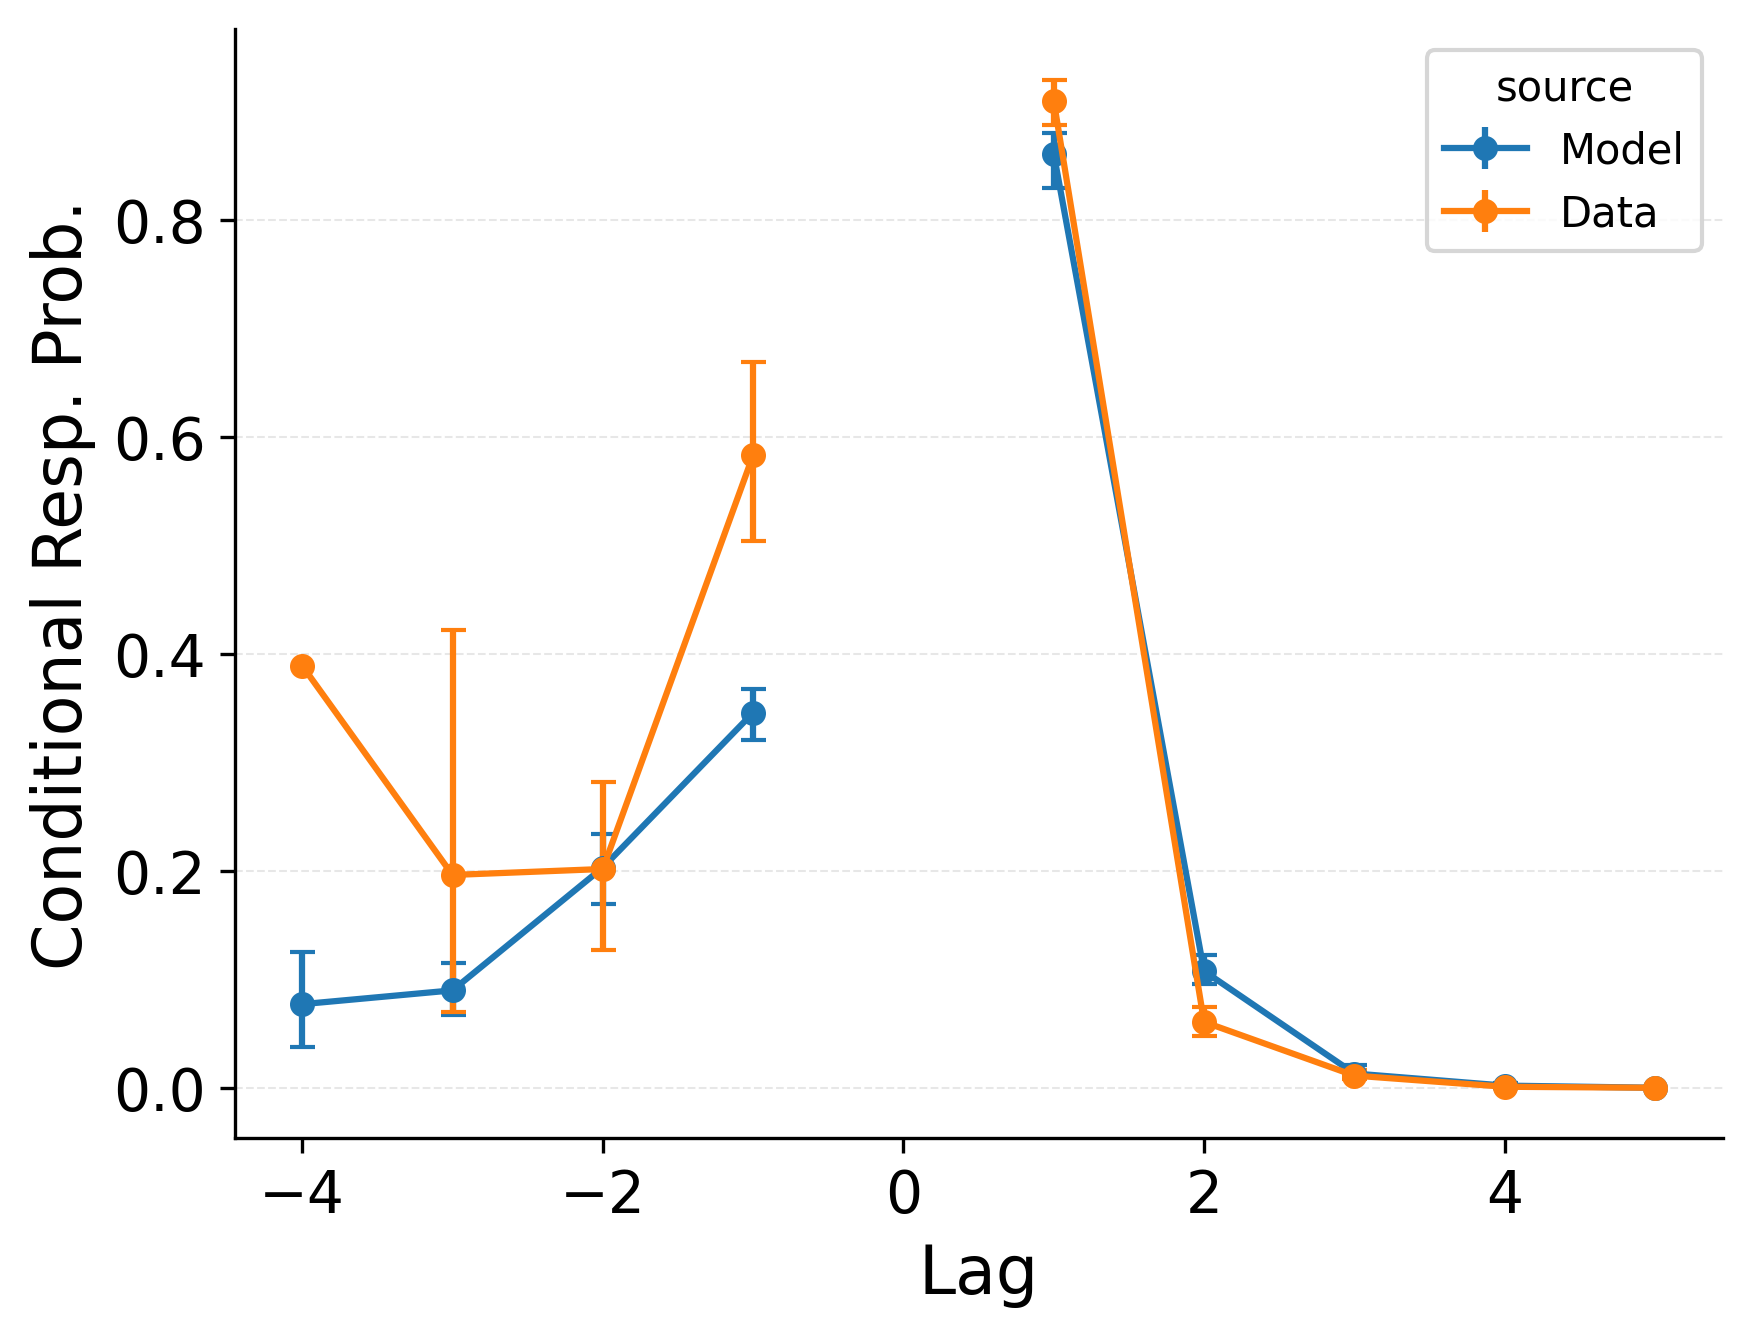
\includegraphics{figures/Gordon2021_BaseCRU_with_ContextTerm_Confusable_Fitting_crp_LL5.png}\end{minipage}%
%
\begin{minipage}{0.33\linewidth}
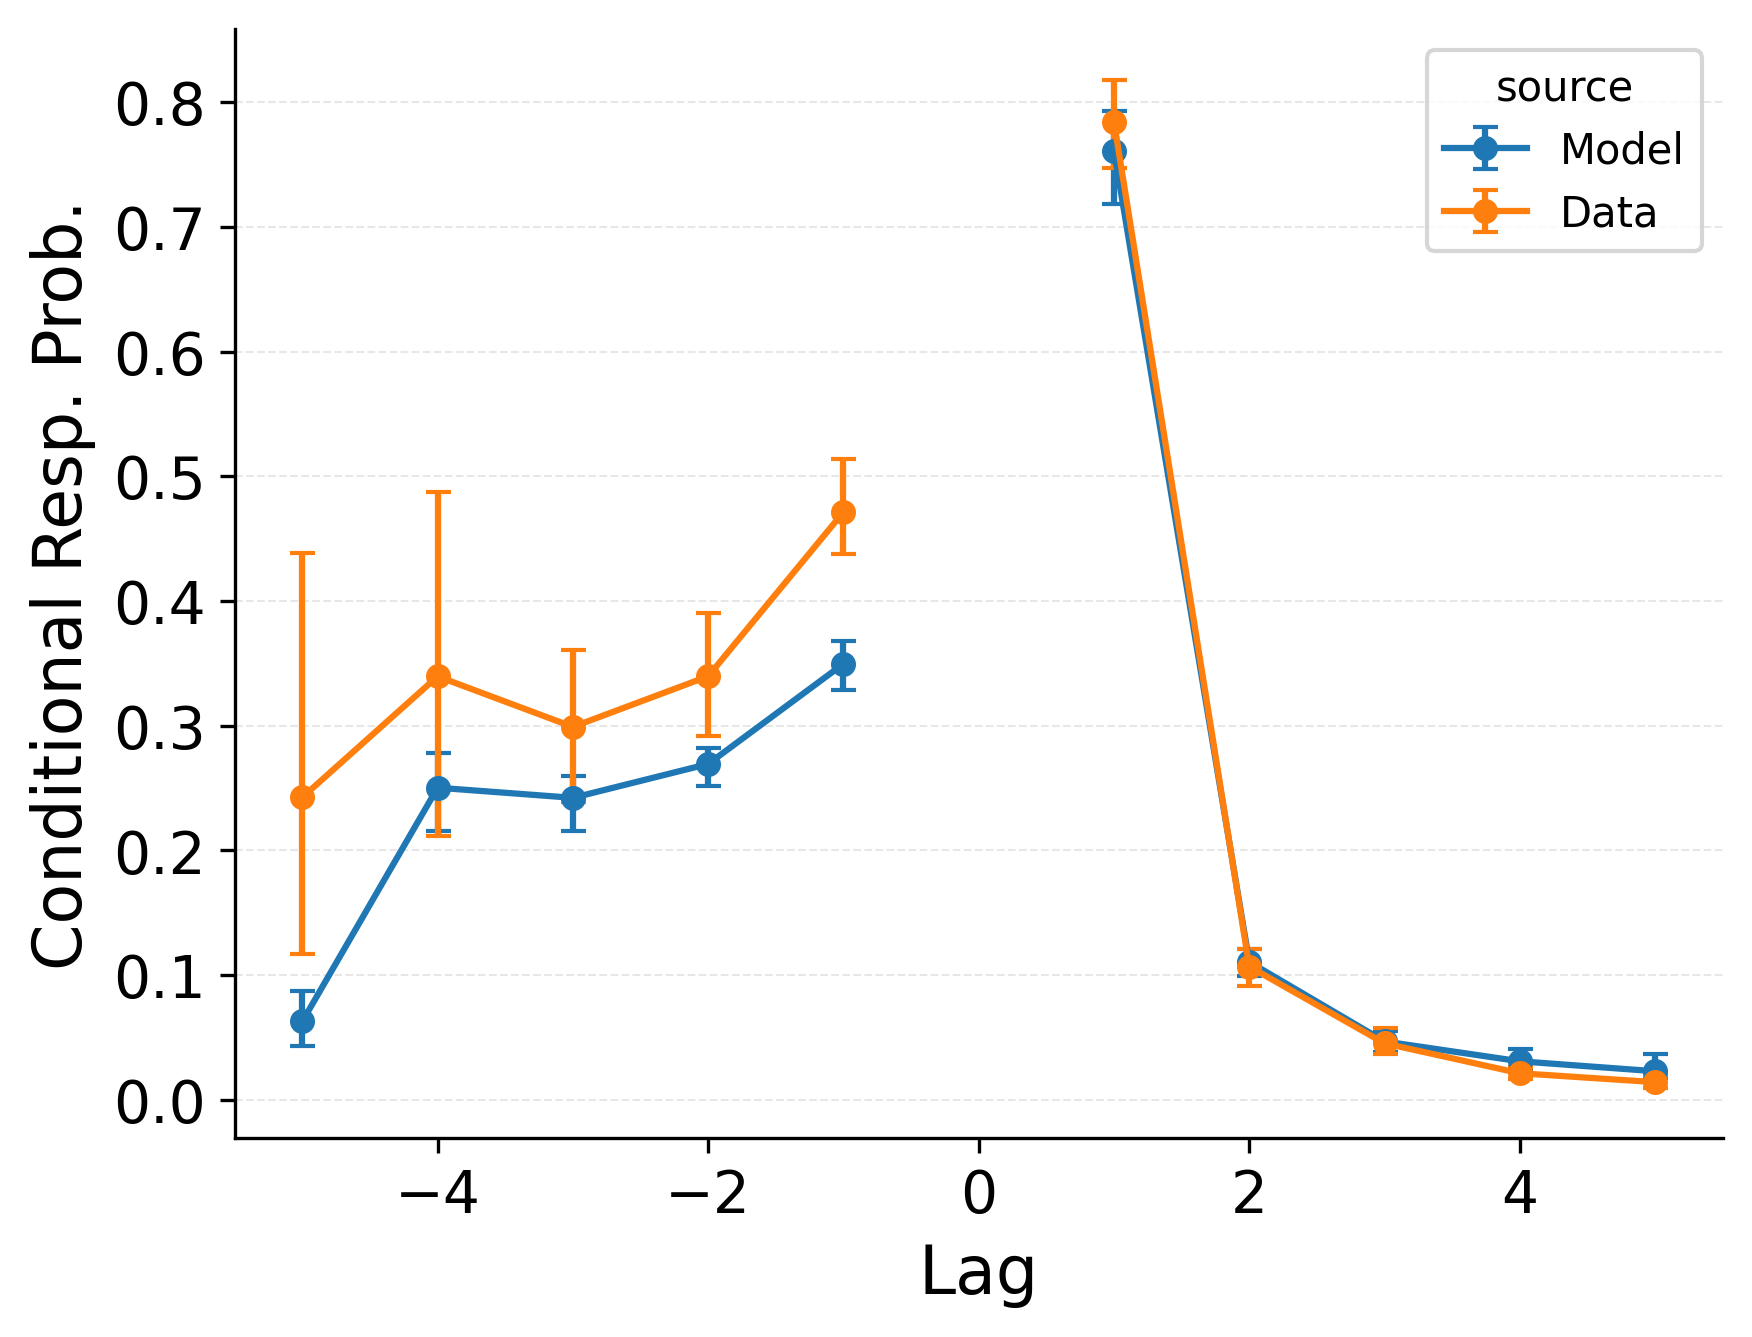
\includegraphics{figures/Gordon2021_BaseCRU_with_ContextTerm_Confusable_Fitting_crp_LL6.png}\end{minipage}%
%
\begin{minipage}{0.33\linewidth}
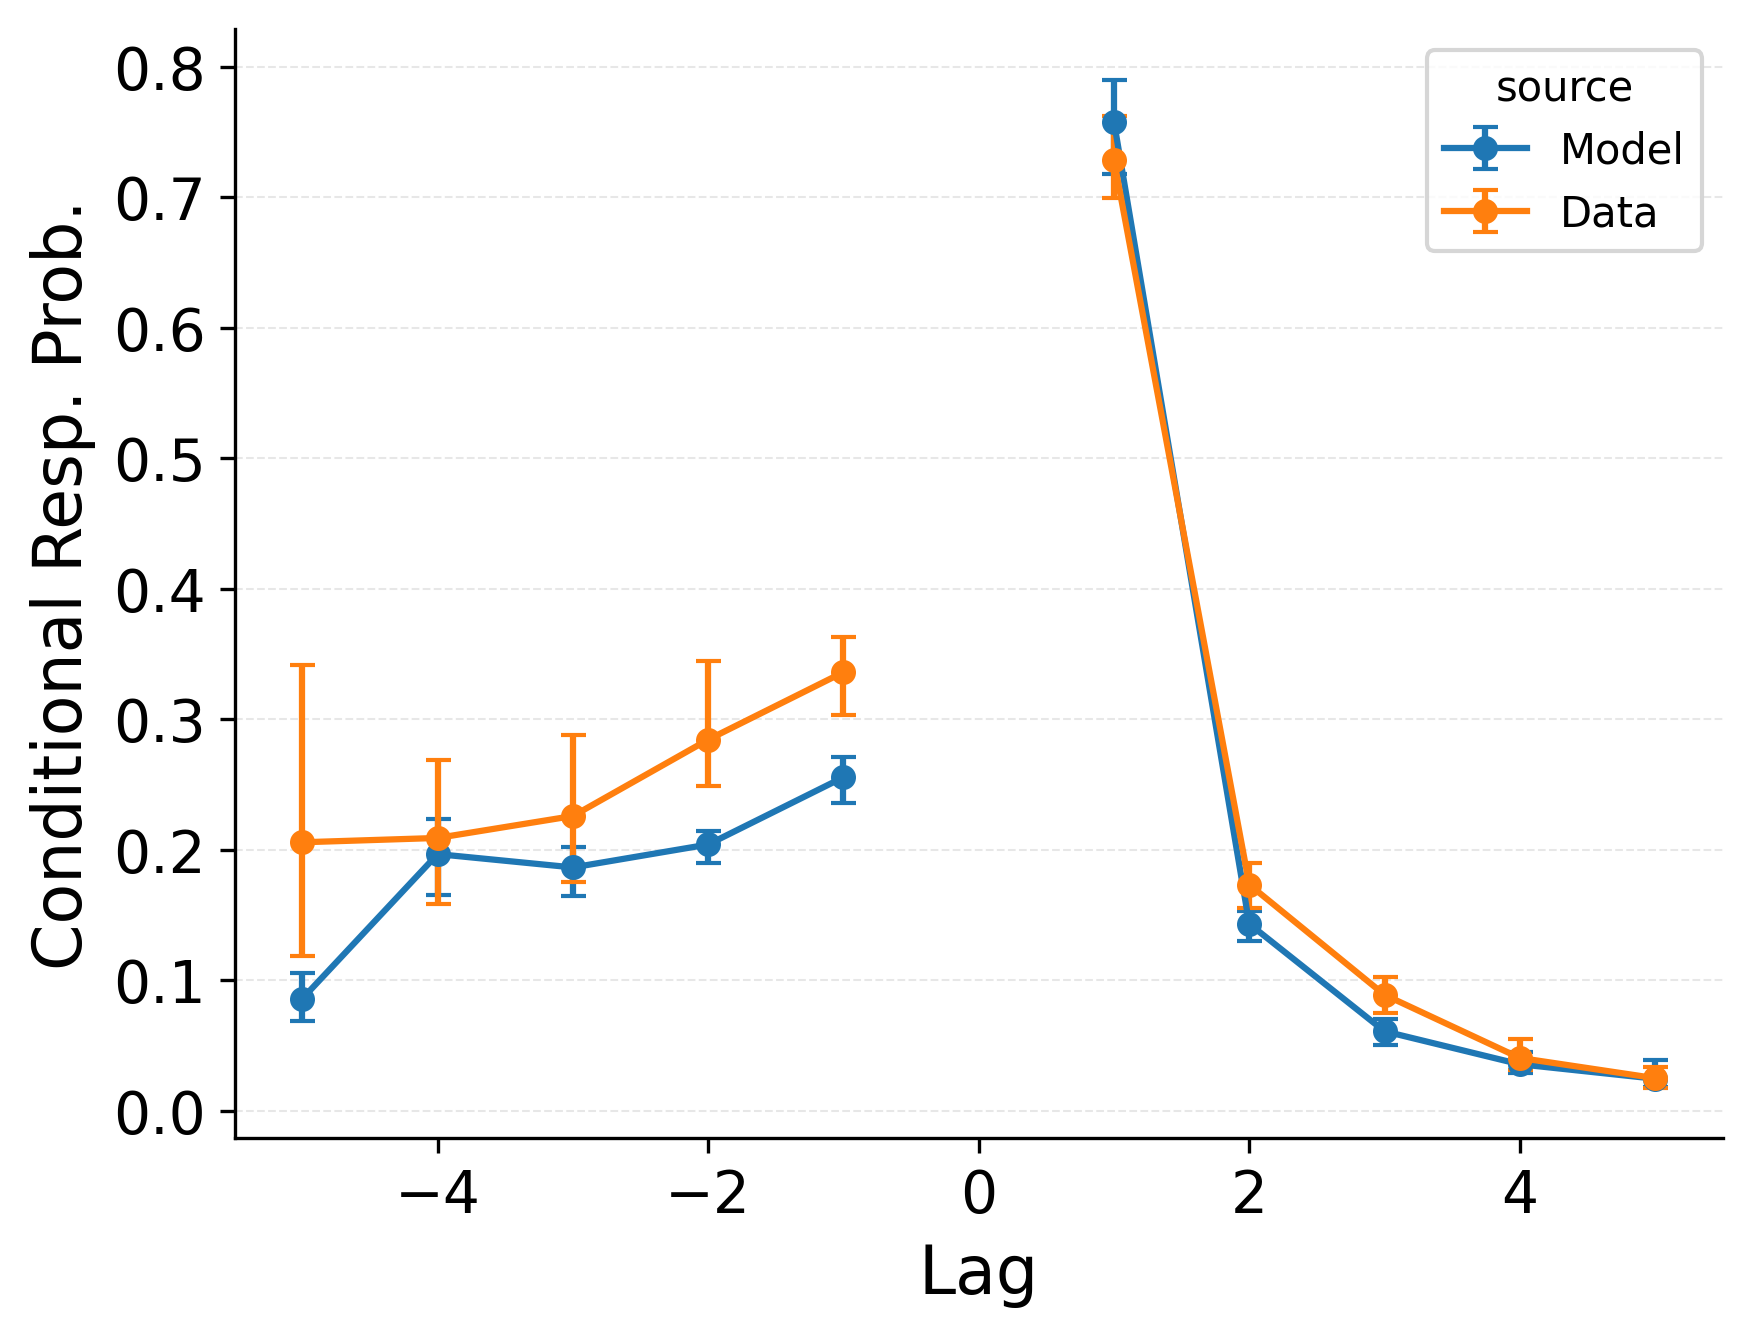
\includegraphics{figures/Gordon2021_BaseCRU_with_ContextTerm_Confusable_Fitting_crp_LL7.png}\end{minipage}%
\newline
\begin{minipage}{0.33\linewidth}
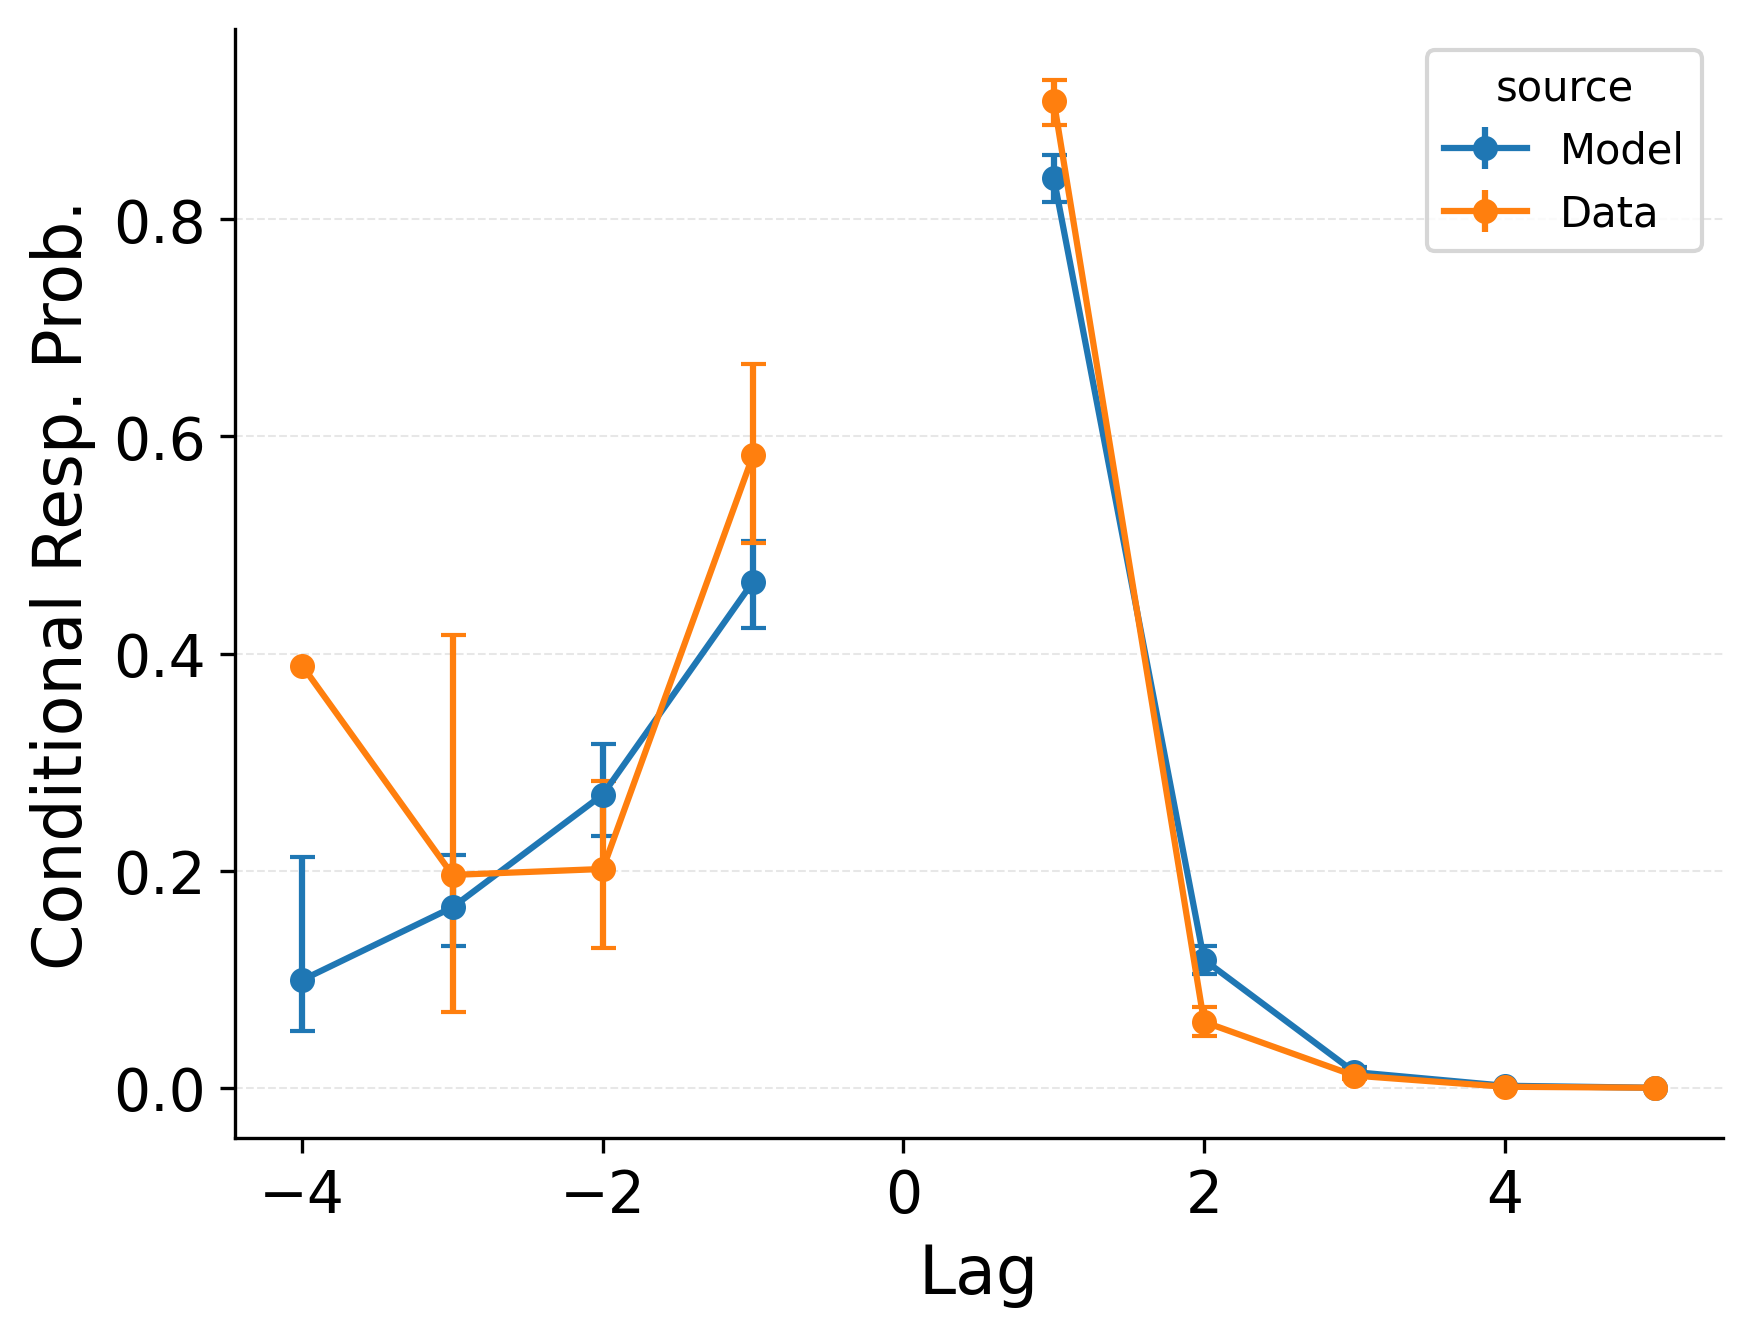
\includegraphics{figures/Gordon2021_CRU_with_Pre-Expt_and_Primacy__and_ContextTerm_Confusable_Fitting_crp_LL5.png}\end{minipage}%
%
\begin{minipage}{0.33\linewidth}
\includegraphics{figures/Gordon2021_CRU_with_Pre-Expt_and_Primacy__and_ContextTerm_Confusable_Fitting_crp_LL6.png}\end{minipage}%
%
\begin{minipage}{0.33\linewidth}
\includegraphics{figures/Gordon2021_CRU_with_Pre-Expt_and_Primacy__and_ContextTerm_Confusable_Fitting_crp_LL7.png}\end{minipage}%
\newline
\begin{minipage}{0.33\linewidth}
\includegraphics{figures/Gordon2021_BaseCMR_Confusable_Fitting_crp_LL5.png}\end{minipage}%
%
\begin{minipage}{0.33\linewidth}
\includegraphics{figures/Gordon2021_BaseCMR_Confusable_Fitting_crp_LL6.png}\end{minipage}%
%
\begin{minipage}{0.33\linewidth}
\includegraphics{figures/Gordon2021_BaseCMR_Confusable_Fitting_crp_LL7.png}\end{minipage}%

\end{figure}%

Serial recall and free recall both show clear temporal structure in
participant's sequence of recall transitions, as characterized by the
lag-CRP analysis. In strict serial recall, participants typically move
forward through the list (i.e., +1 transitions are highly likely), yet
small but reliable rates of backward transitions (e.g., fill-in errors)
are nonetheless observed. These fill-in errors occur when a participant
temporarily skips a position but later ``fill in'' the item that was
missed, effectively jumping backward one or more steps. Just as in free
recall, CMR's feature-to-context memory (\(\gamma\)) and
pre-experimental context-to-feature associations (\(\alpha\),
\(\delta\)) provide a means for reinstating earlier list context,
thereby increasing the model's propensity for backward transitions at
short lags. Lohnas (\citeproc{ref-lohnas2024retrieved}{2024}) observed
this capability in an evaluation of CMR for serial recall, but CRU was
found by Logan (\citeproc{ref-logan2021serial}{2021}) to also capture
applicable backward transitions in the serial recall task.

Our simulations of the lag-CRP confirm that CMR's mechanisms can help
capture these backward transitions Figure~\ref{fig-serial-crp}. Baseline
CRU (top row; with \(\gamma=0\) and \(\alpha, \delta=0\)) underpredicts
the conditional response probability of short backward lags, mirroring
its shortfall in free recall. Hence, when CRU is extended to include the
same associative mechanisms that CMR uses to promote backward
transitions, it better approximates the observed lag-CRP profile in
serial recall. Figure~\ref{fig-serial-crp} (middle row) shows the
lag-CRP for the best performing CRU variant with free pre-experimental
context-to-feature memory (\(\alpha\), \(\delta\)) and CMR-specific
primacy gradient (\(\phi_\text{s}\), \(\phi_\text{d}\)) parameters.

\subsection{An Advantage for Context-Based Recall Termination in Serial
Recall}\label{an-advantage-for-context-based-recall-termination-in-serial-recall}

In our free recall evaluation, we found that CMR's position-based
termination mechanism outperformed CRU's context-based termination
mechanism. This is because the latter can lead to premature termination
when recall initiates with a strong recency effect, as is common in free
recall. However, in our serial recall evaluation, we find that embedding
CRU's context-based termination in CMR improves overall model fits,
despite dropping two free parameters Table~\ref{tbl-fits-serial}. The
standard CMR recall termination mechanism underestimates recall rates
for later list items, as shown in Figure~\ref{fig-serial-srac}.

In serial recall, recall termination is not a function of the number of
recalls made, but rather a function of the current state of the context,
as predicted by CRU's unique specification. By tying the end-of-list
state to the evolving context, CRU effectively models this behavior with
zero additional parameters. In contrast, CMR's exponential growth in
stop probability often forces the model either to under- or overshoot
the actual stopping point. Resolving this discrepancy may require a more
complex model of recall termination that either incorporates insights
from both the context-based and position-based mechanisms or that allows
for strategic control over recall termination depending on the task at
hand.

\section{Discussion}\label{discussion}

The simulation analyses presented here provide a structured comparison
of CRU and CMR in the domain of free recall. CRU is a successful model
of serial recall performance (\citeproc{ref-logan2018automatic}{Logan,
2018}, \citeproc{ref-logan2021serial}{2021};
\citeproc{ref-logan2021bserial}{Logan \& Cox, 2021}). As such, comparing
the two frameworks gives insight into how specific model mechanisms
contribute to behavioral phenomena that differ between the two tasks. At
the outset, we noted how CRU's success in strictly ordered memory tasks
might obscure its capacity to handle the broader dynamics of free
recall, where retrieval can proceed in many directions and often
terminates in flexible ways. By systematically enabling or disabling
different mechanisms from CMR excluded from CRU, we showed how features
like a dynamic feature-to-context memory, pre-experimental
context-to-feature associations, serial position memory strength
scaling, flexible recall initiation, and different termination rules can
critically shape free recall performance. This analysis reveals that CRU
can, in fact, capture many hallmark free recall phenomena when
progressively endowed with CMR-like machinery -- but in so doing, it
gradually converges on CMR's complexity.

By contrast, in our serial recall evaluation, we found that CRU can be
substantially improved with the incorporation of certain CMR mechanisms.
These mechanisms provide a substantial improvement in overall
log-likelihood goodness of fit scores. CRU's streamlined architecture is
sufficient to capture key serial recall phenomena, but incorporation of
these CMR mechanisms yields small improvements in fit to several
phenomena. In contrast to the free recall evaluation, CRU's
context-based recall termination mechanism substantially outperformed
CMR's position-based termination mechanism. Furthermore, CRU's item
identification confusability mechanism was both necessary to capture
intrusion errors in serial recall, and sufficient to capture the
distribution of order and omission errors across study positions.

Particularly in free recall, the factorial approach underscores the
specific changes needed for CRU to handle backward transitions and and
robust primacy--recency trade-offs. The strongest free recall benefits
benefits emerge when we grant CRU the ability to initiate recall
flexibly (\(\beta_\text{start}\)) using a mix of final and initial study
context, a feature that CMR uses to balance primacy and recency effects
in recall initiation (\citeproc{ref-kragel2015neural}{Kragel et al.,
2015}; \citeproc{ref-morton2016predictive}{Morton \& Polyn, 2016}). CMR
additionally implements a proposal by Sederberg et al.
(\citeproc{ref-sederberg2008context}{2008}) that the primacy effect is
supported by increased attention to initial items in study lists.
Implementing this associative primacy gradient by allowing the strength
of context-to-item associations to scale with serial position
(\(\phi_\text{s}, \phi_\text{d}\)) yields appreciable improvements to
CRU when paired with \(\beta_\text{start}\), suggesting that mechanisms
specific to recall initiation and encoding dynamics are crucial for
capturing the shape of serial position curve. Broader research focused
on patterns of response time distributions in free recall initiation
(\citeproc{ref-osth2019using}{Osth \& Farrell, 2019}) suggests that the
balance between primacy and recency effects is a key determinant of
recall initiation dynamics.

Our results confirm that CMR can be adapted to capture intrusion errors
in serial recall by borrowing CRU's confusability mechanism using its
\(g\) and \(g_\text{dec}\) parameters, simultaneously addressing serial
position effects. The mechanism could not evaluated in free recall, as
the mechanism depends on empirical perceptual confusability statistics
across items, which are not available in word-list free recall. However,
the mechanism is likely to be useful in free recall as well, and may be
extended to word lists by using a different set of perceptual
confusability statistics. Future work should examine the generality of
this mechanism across tasks and item sets.

While introducing this flexibility helps CRU capture serial position
effects in free recall, additional mechanisms are needed to fully
capture the bidirectional lag-contiguity effect, though this is not so
much the case in serial recall. Adding pre-experimental associations to
CRU's context-to-feature memory (\(\alpha, \delta\)) provide the
flexibility needed to capture forward transitions in the lag-contiguity
effect. To also capture the strength of backward transitions, CRU needs
to enable feature-to-context learning (\(\gamma\)) so that associations
necessary for contacting backward neighbors can be leveraged during
retrieval. While addressing backward transitions is crucial for
addressing the asymmetric lag-contiguity effect in free recall, such
mechanisms may also help address performance in serial recall where
probed recall of serial lists
(\citeproc{ref-kahana2002associative}{Kahana \& Caplan, 2002}) and
dissociations between forward and backward recall
(\citeproc{ref-li1993intralist}{Li \& Lewandowsky, 1993}) suggest a
similar pattern of associative asymmetry in memory search
(\citeproc{ref-howard2002distributed}{Howard \& Kahana, 2002}).

Prior work examining CMR's ability to capture serial recall phenomena
have proposed that free vs.~serial recall differences reflect a
task-specific configuration of the \(\gamma\) parameter
(\citeproc{ref-lohnas2024retrieved}{Lohnas, 2024}). Our investigation
demonstrates that enabling this mechanism along with pre-experimental
context-to-feature memory parameters (\(\alpha, \delta\)) does improves
CRU's ability to simulate backward transitions in serial recall, but
also shows that CRU already captures the basic effect without using
these mechanisms. Further research is needed to determine whether this
dynamic feature-to-context memory is necessary for capturing performance
in other memory tasks.

Finally, CRU's method of modeling recall termination was poorly aligned
with the variable stopping patterns often observed in free recall. By
contrast, CMR's position-based termination mechanism struggled to
address recall termination dynamics in serial recall, where participants
typically initiate recall with the first item of the list and apparently
treat reaching the end of the list as the main cue to terminate
retrieval. These results reinforce that a purely context-driven account
of termination is better suited to tasks where participants explicitly
strive for sequential order. Even in free recall, other research has
shown that recall termination probability in depends on factors other
than output position. Participants are especially likely to terminate
free recall after making an error
(\citeproc{ref-miller2012recall}{Miller et al., 2012};
\citeproc{ref-unsworth2011factors}{Unsworth et al., 2011}), when they
are less confident in their responses
(\citeproc{ref-unsworth2011factors}{Unsworth et al., 2011}), when they
are less motivated to continue
(\citeproc{ref-dougherty2007motivated}{Dougherty \& Harbison, 2007}),
and when a longer amount of time has passed since the last recall
(\citeproc{ref-dougherty2007motivated}{Dougherty \& Harbison, 2007}).
These results together suggest that recall termination probability is a
function of the difficulty of continuing recall, not just the number of
recalls made so far. Future work may explain these patterns by relating
the accessibility in memory of the next item as predicted by a
retrieved-context model to the likelihood of continuing or terminating
recall. Moreover, this suggests that the shift from using a leaky
competitive accumulation process to a probabilistic termination process
was a theoretical step backwards for CMR, as the accumulation process
more naturally accounts for the relationship between memory
accessibility and successful recall.

By showing that CRU and CMR can be seen as points along a continuum of
retrieved-context approaches, our results highlight both the flexibility
of retrieved-context theory, and the trade-offs involved in simplifying
this theory. CRU's architecture is well-tailored to domains emphasizing
forward-ordered retrieval, but omits parameters crucial for capturing
the bidirectional and open-ended nature of free recall. Meanwhile, CMR's
greater flexibility comes at the cost of added complexity. The results
here do not explore potential overfitting, but suggest that each model
can be expanded or trimmed depending on task demands. Moreover, CRU's
instance-based storage of item--context pairs diverges from CMR's linear
associative memory, and the consequences of this difference for model
behavior are ambiguous pending further research
(\citeproc{ref-anderson1995introduction}{J. A. Anderson, 1995};
\citeproc{ref-turner2019toward}{Turner, 2019}). While both models have
been shown to address item repetitions and out-of-list intrusions (e.g.,
\citeproc{ref-logan2021serial}{Logan, 2021};
\citeproc{ref-siegel2014retrieved}{Siegel \& Kahana, 2014}), it remains
unclear which framework better scales across task domains to address the
full range of memory phenomena. Comparing serial and free recall
performance across a wider range of list lengths and item sets should
clarify the practical boundaries of each approach.

The present analysis sidesteps comparison of CRU and CMR's distinct
recall competition mechanisms based on the justification that neither
model is committed to a specific mechanism for recall competition
(\citeproc{ref-logan2021serial}{Logan, 2021};
\citeproc{ref-morton2016predictive}{Morton \& Polyn, 2016};
\citeproc{ref-polyn2009context}{Polyn et al., 2009}) and simulation
using the probabilistic choice rule is more computationally efficient.
Nonetheless, with response time distributions providing important
constraints for accounts of recall initiation (e.g.,
\citeproc{ref-osth2019using}{Osth \& Farrell, 2019}) and termination
(e.g., \citeproc{ref-dougherty2007motivated}{Dougherty \& Harbison,
2007}), the racing diffusion model of recall competition favored in
demonstrations of CRU (\citeproc{ref-logan2018automatic}{Logan, 2018},
\citeproc{ref-logan2021serial}{2021}) potentially offers a tractable
framework for addressing response time distributions as a theoretical
constraint within the likelihood-based fitting approach used here
(\citeproc{ref-tillman2020sequential}{Tillman et al., 2020}). To benefit
from this approach, future work should clarify assumptions about when
recall competitions begin and end across responses in free and serial
recall tasks, and how these assumptions can be tested against response
time data (\citeproc{ref-logan2021serial}{Logan, 2021}).

In broader terms, these findings advance our understanding of how
context-based models can unify disparate memory phenomena. Indeed, this
ambition follows a long line of Gordon Logan's work, which
systematically shows that a single cognitive architecture can explain
performance across tasks as diverse as visual search, typing, and serial
recall. The parallels we draw between CRU and CMR suggest a shared
foundation for modeling recall sequences, whether strictly ordered as in
serial recall or unconstrained as in free recall. Contemporaneous
research indicates that CMR variants can capture core aspects of both
free and serial recall (\citeproc{ref-lohnas2024retrieved}{Lohnas,
2024}), while CRU's success spans traditional list-learning tasks and
broader cognitive-control or motor-sequencing paradigms that rely on
forward-chained retrieval (\citeproc{ref-logan2018automatic}{Logan,
2018}, \citeproc{ref-logan2021serial}{2021}). Such breadth underscores
the remarkable scope of retrieved-context theory as a unifying
explanation across multiple domains, from free recall of word lists to
hierarchical production skills. By situating CRU and CMR within a single
modeling space, we emphasize how closely related mechanisms can produce
seemingly divergent behaviors. This convergence invites researchers to
treat free and serial recall findings as complementary constraints on a
unified account of memory search, laying groundwork for a more
integrated theory of episodic retrieval in both highly directed and more
open-ended recall scenarios.

\section{References}\label{references}

\phantomsection\label{refs}
\begin{CSLReferences}{1}{0}
\bibitem[\citeproctext]{ref-anderson1995introduction}
Anderson, J. A. (1995). \emph{An introduction to neural networks}. MIT
press.

\bibitem[\citeproctext]{ref-anderson1972recognition}
Anderson, J. R., \& Bower, G. H. (1972). Recognition and retrieval
processes in free recall. \emph{Psychological Review}, \emph{79}(2), 97.

\bibitem[\citeproctext]{ref-dougherty2007motivated}
Dougherty, M. R., \& Harbison, J. (2007). Motivated to retrieve: How
often are you willing to go back to the well when the well is dry?
\emph{Journal of Experimental Psychology: Learning, Memory, and
Cognition}, \emph{33}(6), 1108.

\bibitem[\citeproctext]{ref-estes1955statistical}
Estes, W. K. (1955). Statistical theory of spontaneous recovery and
regression. \emph{Psychological Review}, \emph{62}(3), 145.

\bibitem[\citeproctext]{ref-friendly1982toronto}
Friendly, M., Franklin, P. E., Hoffman, D., \& Rubin, D. C. (1982). The
toronto word pool: Norms for imagery, concreteness, orthographic
variables, and grammatical usage for 1,080 words. \emph{Behavior
Research Methods \& Instrumentation}, \emph{14}(4), 375--399.

\bibitem[\citeproctext]{ref-healey2014memory}
Healey, M. K., \& Kahana, M. J. (2014). Is memory search governed by
universal principles or idiosyncratic strategies? \emph{Journal of
Experimental Psychology: General}, \emph{143}(2), 575.

\bibitem[\citeproctext]{ref-healey2016four}
Healey, M. K., \& Kahana, M. J. (2016). A four-component model of
age-related memory change. \emph{Psychological Review}, \emph{123}(1),
23.

\bibitem[\citeproctext]{ref-healey2024peppr}
Healey, M. K., \& Wahlheim, C. N. (2024). PEPPR: A post-encoding
pre-production reinstatement model of dual-list free recall.
\emph{Memory \& Cognition}, \emph{52}(1), 163--181.

\bibitem[\citeproctext]{ref-hong2024modulation}
Hong, M. K., Gunn, J. B., Fazio, L. K., \& Polyn, S. M. (2024). The
modulation and elimination of temporal organization in free recall.
\emph{Journal of Experimental Psychology: Learning, Memory, and
Cognition}, \emph{50}(7), 1035.

\bibitem[\citeproctext]{ref-horwath2023value}
Horwath, E. A., Rouhani, N., DuBrow, S., \& Murty, V. P. (2023). Value
restructures the organization of free recall. \emph{Cognition},
\emph{231}, 105315.

\bibitem[\citeproctext]{ref-howard1999context}
Howard, M. W., \& Kahana, M. J. (1999). Contextual variability and
serial position effects in free recall. \emph{Journal of Experimental
Psychology: Learning, Memory, and Cognition}, \emph{25}(4), 923.

\bibitem[\citeproctext]{ref-howard2002distributed}
Howard, M. W., \& Kahana, M. J. (2002). A distributed representation of
temporal context. \emph{Journal of Mathematical Psychology},
\emph{46}(3), 269--299.

\bibitem[\citeproctext]{ref-kahana1996associative}
Kahana, M. J. (1996). Associative retrieval processes in free recall.
\emph{Memory \& Cognition}, \emph{24}(1), 103--109.

\bibitem[\citeproctext]{ref-kahana2020computational}
Kahana, M. J. (2020). Computational models of memory search.
\emph{Annual Review of Psychology}, \emph{71}(1), 107--138.

\bibitem[\citeproctext]{ref-kahana2002associative}
Kahana, M. J., \& Caplan, J. B. (2002). Associative asymmetry in probed
recall of serial lists. \emph{Memory \& Cognition}, \emph{30}(6),
841--849.

\bibitem[\citeproctext]{ref-kragel2015neural}
Kragel, J. E., Morton, N. W., \& Polyn, S. M. (2015). Neural activity in
the medial temporal lobe reveals the fidelity of mental time travel.
\emph{Journal of Neuroscience}, \emph{35}(7), 2914--2926.

\bibitem[\citeproctext]{ref-li1993intralist}
Li, S.-C., \& Lewandowsky, S. (1993). Intralist distractors and recall
direction: Constraints on models of memory for serial order.
\emph{Journal of Experimental Psychology: Learning, Memory, and
Cognition}, \emph{19}(4), 895.

\bibitem[\citeproctext]{ref-logan1988toward}
Logan, G. D. (1988). Toward an instance theory of automatization.
\emph{Psychological Review}, \emph{95}(4), 492.

\bibitem[\citeproctext]{ref-logan2018automatic}
Logan, G. D. (2018). Automatic control: How experts act without
thinking. \emph{Psychological Review}, \emph{125}(4), 453.

\bibitem[\citeproctext]{ref-logan2021serial}
Logan, G. D. (2021). Serial order in perception, memory, and action.
\emph{Psychological Review}, \emph{128}(1), 1.

\bibitem[\citeproctext]{ref-logan2021bserial}
Logan, G. D., \& Cox, G. E. (2021). Serial memory: Putting chains and
position codes in context. \emph{Psychological Review}, \emph{128}(6),
1197.

\bibitem[\citeproctext]{ref-logan2023serial}
Logan, G. D., \& Cox, G. E. (2023). Serial order depends on
item-dependent and item-independent contexts. \emph{Psychological
Review}.

\bibitem[\citeproctext]{ref-logan2001executive}
Logan, G. D., \& Gordon, R. D. (2001). Executive control of visual
attention in dual-task situations. \emph{Psychological Review},
\emph{108}(2), 393.

\bibitem[\citeproctext]{ref-lohnas2024retrieved}
Lohnas, L. J. (2024). A retrieved context model of serial recall and
free recall. \emph{Computational Brain \& Behavior}, 1--35.

\bibitem[\citeproctext]{ref-lohnas2015expanding}
Lohnas, L. J., Polyn, S. M., \& Kahana, M. J. (2015). Expanding the
scope of memory search: Modeling intralist and interlist effects in free
recall. \emph{Psychological Review}, \emph{122}(2), 337.

\bibitem[\citeproctext]{ref-luce1959individual}
Luce, R. D. (1959). \emph{Individual choice behavior} (Vol. 4). Wiley
New York.

\bibitem[\citeproctext]{ref-melton1972coding}
Melton, A. W., \& Martin, E. (1972). \emph{Coding processes in human
memory.}

\bibitem[\citeproctext]{ref-miller2012recall}
Miller, J. F., Weidemann, C. T., \& Kahana, M. J. (2012). Recall
termination in free recall. \emph{Memory \& Cognition}, \emph{40},
540--550.

\bibitem[\citeproctext]{ref-morton2016predictive}
Morton, N. W., \& Polyn, S. M. (2016). A predictive framework for
evaluating models of semantic organization in free recall. \emph{Journal
of Memory and Language}, \emph{86}, 119--140.

\bibitem[\citeproctext]{ref-murdock1962serial}
Murdock, B. B. (1962). The serial position effect of free recall.
\emph{Journal of Experimental Psychology}, \emph{64}(5), 482.

\bibitem[\citeproctext]{ref-osth2019using}
Osth, A. F., \& Farrell, S. (2019). Using response time distributions
and race models to characterize primacy and recency effects in free
recall initiation. \emph{Psychological Review}, \emph{126}(4), 578.

\bibitem[\citeproctext]{ref-osth2023item}
Osth, A. F., \& Hurlstone, M. J. (2023). \emph{Do item-dependent context
representations underlie serial order in cognition? Commentary on logan
(2021).}

\bibitem[\citeproctext]{ref-polyn2023assessing}
Polyn, S. M. (2023). Assessing neurocognitive hypotheses in a
likelihood-based model of the free-recall task. In \emph{An introduction
to model-based cognitive neuroscience} (pp. 303--325). Springer.

\bibitem[\citeproctext]{ref-polyn2009context}
Polyn, S. M., Norman, K. A., \& Kahana, M. J. (2009). A context
maintenance and retrieval model of organizational processes in free
recall. \emph{Psychological Review}, \emph{116}(1), 129.

\bibitem[\citeproctext]{ref-sederberg2011human}
Sederberg, P. B., Gershman, S. J., Polyn, S. M., \& Norman, K. A.
(2011). Human memory reconsolidation can be explained using the temporal
context model. \emph{Psychonomic Bulletin \& Review}, \emph{18},
455--468.

\bibitem[\citeproctext]{ref-sederberg2008context}
Sederberg, P. B., Howard, M. W., \& Kahana, M. J. (2008). A
context-based theory of recency and contiguity in free recall.
\emph{Psychological Review}, \emph{115}(4), 893.

\bibitem[\citeproctext]{ref-siegel2014retrieved}
Siegel, L. L., \& Kahana, M. J. (2014). A retrieved context account of
spacing and repetition effects in free recall. \emph{Journal of
Experimental Psychology: Learning, Memory, and Cognition}, \emph{40}(3),
755.

\bibitem[\citeproctext]{ref-storn1997differential}
Storn, R., \& Price, K. (1997). Differential evolution--a simple and
efficient heuristic for global optimization over continuous spaces.
\emph{Journal of Global Optimization}, \emph{11}(4), 341--359.

\bibitem[\citeproctext]{ref-tillman2020sequential}
Tillman, G., Van Zandt, T., \& Logan, G. D. (2020). Sequential sampling
models without random between-trial variability: The racing diffusion
model of speeded decision making. \emph{Psychonomic Bulletin \& Review},
\emph{27}(5), 911--936.

\bibitem[\citeproctext]{ref-tulving1970memory}
Tulving, E., \& Madigan, S. A. (1970). Memory and verbal learning.
\emph{Annual Review of Psychology}, \emph{21}, 437--484.

\bibitem[\citeproctext]{ref-turner2019toward}
Turner, B. M. (2019). Toward a common representational framework for
adaptation. \emph{Psychological Review}, \emph{126}(5), 660.

\bibitem[\citeproctext]{ref-unsworth2011factors}
Unsworth, N., Brewer, G. A., \& Spillers, G. J. (2011). Factors that
influence search termination decisions in free recall: An examination of
response type and confidence. \emph{Acta Psychologica}, \emph{138}(1),
19--29.

\bibitem[\citeproctext]{ref-zhang2023optimal}
Zhang, Q., Griffiths, T. L., \& Norman, K. A. (2023). Optimal policies
for free recall. \emph{Psychological Review}, \emph{130}(4), 1104.

\end{CSLReferences}






\end{document}
